\documentclass{include/thesisclass}

\SelectLanguage{english}
\newcommand{\thesisauthor}{Marvin-Dennis Noll}
\newcommand{\thesistopic}{Stability Improvements at FLUTE}
\newcommand{\thesisentopic}{Verbesserung der Stabilität von FLUTE}
\newcommand{\thesislongtopic}{}
\newcommand{\thesisinstitute}{Institute for Beam Physics and Technology}
\newcommand{\thesisreviewerone}{Prof. Dr.-Ing. John Jelonnek (IHM)}
\newcommand{\thesisreviewertwo}{Prof. Dr. Anke-Susanne Müller (IBPT)}
\newcommand{\thesisadvisorone}{Dr. Nigel Smale (IBPT)} % to use: enter names and uncomment in titlepg
\newcommand{\thesisadvisortwo}{}
\newcommand{\thesistimestart}{15.11.2020} % on titlepage
\newcommand{\thesistimeend}{12.05.2021} % on titlepage
\newcommand{\thesistimehandin}{10.05.2021} % on second page 'preamble'
\newcommand{\thesispagehead}{Master Thesis: \thesisentopic} % page heading

\hypersetup
{
    pdfauthor={\thesisauthor},
    pdftitle={Masterarbeit: \thesistopic},
    pdfsubject={\thesislongtopic},
    pdfkeywords={kit,physics,master,thesis,\thesisauthor}
}

%my imports
\usepackage{hyperref}
\usepackage{amsmath}
\usepackage{siunitx}
\usepackage{float}
\usepackage{tabularx}
\usepackage{tikzscale}
\usepackage{pgfplots}
\pgfplotsset{compat=newest}
\usetikzlibrary{external}
\usetikzlibrary{shapes,arrows.meta}
\tikzexternalize[optimize=false,prefix=tikz/]
\usepackage{listings}
\lstset{
  literate={ö}{{\"o}}1
           {ä}{{\"a}}1
           {ü}{{\"u}}1
           {Ü}{{\"U}}1
           {Ö}{{\"O}}1
           {Ä}{{\"A}}1
}
\definecolor{mygreen}{RGB}{28,172,0} % color values Red, Green, Blue
\definecolor{mylilas}{RGB}{170,55,241}

\lstdefinelanguage{AHDL}
{
	% list of keywords
	morekeywords={
		import,
		if,
		then,
		while,
		for,
		table,
		variable,
		subdesign,
		signal,
		machine,
		of,
		bits,
		with,
		states,
		begin,
		end
	},
	sensitive=false, % keywords are not case-sensitive
	morecomment=[l]{\%} % l is for line comment
	tabsize=2
}

%common settings
%\lstset{
%    breaklines=true,%
%    morekeywords={},
%    keywordstyle=\color{blue},%
%    morekeywords=[2]{1}, keywordstyle=[2]{\color{black}},
%    identifierstyle=\color{black},%
%    stringstyle=\color{mylilas},
%    commentstyle=\color{mygreen},%
%    showstringspaces=false,%without this there will be a symbol in the places where there is a space
%    numbers=left,%
%    numberstyle={\tiny \color{black}},% size of the numbers
%    numbersep=9pt, % this defines how far the numbers are from the text
%    tabsize=2,
%    basicstyle=\footnotesize\ttfamily
%}

%prevent copying line numbers over from pdf
\usepackage{accsupp}
\newcommand{\noncopynumber}[1]{%
    \BeginAccSupp{method=escape,ActualText={}}%
    #1%
    \EndAccSupp{}%
}
%common settings
\lstset{columns=flexible}
\lstset{keepspaces=false}
\lstset{
    breaklines=true,%
    morekeywords={},%
    frame=tb,
    basicstyle={\footnotesize},
    keywordstyle=\bfseries,%
    showstringspaces=false,%without this there will be a symbol in the places where there is a space
    numbers=left,%
    numberstyle=\tiny\noncopynumber,% size of the numbers
    numbersep=9pt, % this defines how far the numbers are from the text
    tabsize=2%  
}


\lstdefinestyle{vhdl}
{
    language=VHDL,%
}

\lstdefinestyle{ahdl}
{
    language=AHDL,%
}

\lstdefinestyle{verilog}
{
    language=Verilog,%
}

\lstdefinestyle{python}
{
    language=Python,%
}







\begin{document}
    % Titlepage and ToC
    \FrontMatter

    \tikzexternaldisable
% coordinates for background border
\newcommand{\diameter}{20}
\newcommand{\xone}{-15}
\newcommand{\xtwo}{160}
\newcommand{\yone}{15}
\newcommand{\ytwo}{-253}




\begin{titlepage}
    % background border
    \begin{tikzpicture}[overlay]
    \draw[color=gray]
            (\xone mm, \yone mm)
      -- (\xtwo mm, \yone mm)
    arc (90:0:\diameter pt)
      -- (\xtwo mm + \diameter pt , \ytwo mm)
        -- (\xone mm + \diameter pt , \ytwo mm)
    arc (270:180:\diameter pt)
        -- (\xone mm, \yone mm);
    \end{tikzpicture}



    % KIT image and sign for faculty of physics
    \begin{textblock}{10}[0,0](4.5,2.5)
        \includegraphics[width=.25\textwidth]{include/kitlogo.pdf}
    \end{textblock}
    \changefont{phv}{m}{n}    % helvetica
    \begin{textblock}{10}[0,0](5.5,2.2)
        \begin{flushright}
            \Large DEPARTMENT OF PHYSICS\\\thesisinstitute
        \end{flushright}
    \end{textblock}



    % horizontal line
    \begin{textblock}{10}[0,0](4.2,3.1)
        \begin{tikzpicture}[overlay]
        \draw[color=gray]
                (\xone mm + 5 mm, -12 mm)
          -- (\xtwo mm + \diameter pt - 5 mm, -12 mm);
        \end{tikzpicture}
    \end{textblock}



    % begin of text part
    \changefont{phv}{m}{n}    % helvetica
    \centering



    % thesis topic (en and ge)
    \vspace*{3cm}
    \Huge\thesistopic\\
    \huge(\thesisentopic)\\



    % author name and institute
    \vspace*{2cm}
    \Large Master thesis\\of\\
    \vspace*{1cm}
    \huge\thesisauthor\\
    \vspace*{1cm}
    \Large at the \thesisinstitute



    % possible frontimage - thanks to JabberWok
    % for publishing the img under GNU Document License
    \vspace*{6.5cm}
    %\includegraphics[scale=0.7]{./include/frontimage.eps}\\



    % examiners (Referenten)
    \vspace*{1.5cm}
    \Large
    \begin{center}
        \begin{tabular}[ht]{l c l}
        \iflanguage{english}{Reviewer}{Referent}: 
            & \hfill & \thesisreviewerone\\
        \iflanguage{english}{Second Reviewer}{Korreferent}: 
            & \hfill & \thesisreviewertwo\\
        % uncomment if you want to provide info on your advisors
        \iflanguage{english}{Advisor}{Betreuender Mitarbeiter}: 
            & \hfill & \thesisadvisorone\\
        %\iflanguage{english}{Second Advisor}{Zweiter betreuender Mitarbeiter}: 
        %    & \hfill & \thesisadvisortwo\\
        \end{tabular}
    \end{center}



    % working time
    \vspace{1cm}
    \begin{center}
        \large{\thesistimestart \hspace*{0.25cm} -- %
                                   \hspace*{0.25cm} \thesistimeend}
    \end{center}



    % lowest text blocks concerning the KIT
    \begin{textblock}{10}[0,0](2,16.8)
        \tiny{KIT – The Research University in the Helmholtz Association}
    \end{textblock}
    \begin{textblock}{10}[0,0](10,16.75)
        \large{\textbf{www.kit.edu}}
    \end{textblock}
\end{titlepage}
\tikzexternalize[optimize=false,prefix=tikz/]

    \chapter*{Erklärung zur Selbstständigkeit}
Ich versichere wahrheitsgemäß, die Arbeit selbstständig angefertigt, alle benutzten Hilfsmittel vollständig und genau angegeben und alles kenntlich gemacht zu haben, was aus Arbeiten anderer unverändert oder mit Abänderungen entnommen wurde und dass ich die Satzung des KIT zur Sicherung guter wissenschaftlicher Praxis in der gültigen Fassung vom 24.05.2018 beachtet habe.\\

\vspace{1cm}

\renewcommand{\arraystretch}{0} % for spacing in the tabular environment

\begin{flushright}
	\begin{tabular}{rr}
		Karlsruhe, den \thesistimehandin, & \hspace*{5cm}\\[0mm]
		\cline{2-2}\\[2mm]    % the last line has height 2mm due
		& \thesisauthor       % to \arraystretch=0
	\end{tabular}
\end{flushright}

\vfill

\begin{flushright}
	Als Prüfungsexemplar genehmigt von\\
	\vspace{1cm}
	\begin{tabular}{rr}
		Karlsruhe, den \thesistimehandin, & \hspace*{5cm}\\[0mm]
		\cline{2-2}\\[2mm]    % the last line has height 2mm due
		& \thesisreviewerone  % to \arraystretch=0
	\end{tabular}
\end{flushright}

\renewcommand{\arraystretch}{1}

\cleardoublepage


    \begingroup \let\clearpage\relax    % in order to avoid listoffigures and
    \tableofcontents                    % listoftables on new pages
    \listoffigures
    \listoftables
    \endgroup
    \cleardoublepage

    % Contents
    \MainMatter

	\section*{Abstract}
The \textbf{F}erninfrarot \textbf{L}inac- \textbf{U}nd \textbf{T}est-\textbf{E}xperiment (FLUTE), a compact linear accelerator, is currently designed and under commission at the Karlsruhe Institute of Technology (KIT). Its main purposes are to serve as a technology platform for accelerator research, the generation of strong and ultra short THz pulses and in the future as an injection device for \textbf{c}ompact \textbf{St}orage ring for \textbf{A}ccelerator \textbf{R}esearch and \textbf{T}echnology (cSTART).

At the current commissioning state, the klystron which powers the electron gun/RF cavity and in later stages the linear accelerator is fed by a pulse forming network, which is driven by a high voltage source connected to mains power. For high and a stable output power of the cavity resonator, several parameters have to be tuned to the correct values and kept inside of sometimes small tolerance bands.\\
In the past, the coolant temperature of the cavities water cooling system and the dependency of the pulse forming network output of the mains voltage phase were predominant sources of instability. After dealing with these issues, the cavity output power stability was improved significantly but further improvements to the stability were still desired.

In this work instead of passively optimizing the stability of system parameters, an active approach is evaluated. By controlling the amplitude of the RF input signal of klystron, which is easily possible since it is low power, the effects of noise and/or drifts are mitigated.\\
Here it is evaluated if a simple of the shelf voltage controllable attenuator is a feasible choice to control the RF input signal, which input data should be used and which algorithm and/or control system is suitable to determine the needed attenuator setting to stabilize RF output (of the cavity).\\
Furthermore since the next stage in the system depends on a stable electron bunch charge rather than cavity power, it is determined whether the charge measurements of a Faraday cup can be used to directly control electron bunch charge.

\section*{Kurzfassung}
--TODO--
	\chapter{Introduction}
\section{FLUTE - Ferninfrarot Linac- und Test-Experiment}
	\chapter{Theoretical Background}
\section{Linear accelerators}
\subsection{RF cavities}
\section{Relevant controlled systems theory}
	\chapter{Problem and Previous Work}
\section{Problem statement}
\section{Previous work}
\subsection{50Hz noise}
\subsection{Stabilizing water temperature}
	\chapter{Machine Diagnostics and Sensors}
Most signals to be useful for diagnostics are available in EPICS. Retrieving their current value is therefore straight forward.

For example using the command line tool \texttt{caget} the last value of a PV can be obtained independent of the programming language used, however a syscall is needed which comes with a (slight) overhead and is inconvenient to use.

At least for Python and C++ there are EPICS libraries directly providing useful EPICS commands. A Python example of how to get the current cavity power is shown in \autoref{lst:sensors-epicscaget}.

\begin{lstlisting}[style=python,caption = Get an EPICS PV with python, label = lst:sensors-epicscaget]
from epics import caget
cavity_power=caget("F:RF:LLRF:01:GunCav1:Power:Out")
\end{lstlisting}

\section{Klystron and Cavity RF power}
The RF power directly out of the klystron and right before the cavity are measured with TODO and available in EPICS.

\section{Water Temperatures}
Certain components of FLUTE that generate a lot of heat when in operation are water cooled. The cooling water temperatures are measured and delivered to EPICS. 

\section{Electron Bunch Charge}
A faraday cup FARC-04\cite{radiabeamFaradayCups} (by RadiaBeam Technologies) is used to measure the charge of an electron bunch.

At the moment it is read out with a PCB 421A25\cite{pcbsynotechPCB421A25Charge} charge amplifier. With the TODO-DAQ the output voltage signal ($\sim$ the charge) is fed into EPICS.






	\chapter{Influencing the LLRF with a RF Attenuator}\label{chap:atten}
A RF attenuator provides a fast and simple way of influencing the RF power delivery without interfering too much with existing subsystems, such as the LLRF MTCA system from DESY.

\FloatBarrier
\section{Requirements}
In order for the attenuator to be useful for its application, some requirements are formulated first (\autoref{tab:atteneval-reqs}).

\begin{table}[tbh!]
	\centering
	\caption{Requirements against the attenuator is evaluated}
	\label{tab:atteneval-reqs}
	\begin{tabular}{ll}
		\toprule
		\textbf{Requirement} & \textbf{Value}\\
		\midrule
		attenuation set point resolution & \SI{0.1}{\dB}\\
		attenuation repeatability  & \SI{0.01}{\dB}\\
		\midrule
		temperature range & TODO \\
		voltage supply range & TODO\\
		\bottomrule
	\end{tabular}
\end{table}

\FloatBarrier
\section{Selection and Overview of the selected Device}
The ZX73-2500-S+ is a voltage controllable RF attenuator with coaxial SMA connectors by Mini-Circuits. As it is the only offering from Mini-Circuits of a RF attenuator with SMA connectors and is similar to devices from other manufactures, it is bought for evaluation.

Internally the ZX73-2500-S+ is based on the Mini Circuits RVA-2500+, a variable SMD attenuator in the DV874 case form factor. According to equivalent circuit in the data sheet in \cite{mini-circuitsZX732500VoltageVariable} it can be assumed it is based on the common quad-$\pi$ pin diode design\cite{waughLowCostSurfaceMount1992}.

To get a first impression of the device capabilities, the attenuation over frequency measurements from the data sheet are repeated but with a higher maximum frequency of \SI{4}{\GHz} instead of \SI{2.5}{\GHz} (the highest frequency for which the attenuator is specified). \autoref{fig:atteneval-overview-NA} shows the result.

\begin{figure}[tb]
	\centering
	\includegraphics[width=\textwidth,height=0.5\textwidth]{chap/5-own-work-actuators/img/atteneval/NA/attenuationOverFrequencyParamVctrl.tikz}
	\caption{Device attenuation vs. RF frequency over DC control voltage;\\ measured with network analyzer (see \ref{app:agilent-e5071c}, parameters: $\#AVG$: 16, $IF\text{-}BW$: \SI{10}{\kHz})}
	\label{fig:atteneval-overview-NA}
\end{figure}

In the next sections an operating point is chosen (only relative changes in attenuation are relevant) and then the influences of environment changes on the attenuation are examined.

\FloatBarrier
\section{Measurement setup}
For all the following sections in this chapter,common measurement setup is needed. It needs to
\begin{itemize}
\item supply the attenuator with the supply voltage $V+$\footnote{To experiment with the influence of the supply voltage on attenuation, this also should be tunable.}
\item feed in the (tunable) control voltage $V_{control}$
\item supply RF power
\item measure the attenuation
\item keep track of $V+$, $V_{control}$ and the temperature $\vartheta_{case}$
\end{itemize}

To achieve this, the setup in \autoref{fig:atteneval-setup} is used. In addition to the shown connection, each device is connected via Ethernet to a network switch and subsequently to a computer which runs a custom python program. Since all lab devices used are VXI11 compatible, they are easy to remote control. So for most measurements needed in this chapter no manual operation of the devices is needed and the program can set all parameters according to the test protocol before doing a measurement.

With the setup, a measurement frequency of about \SI{0.5}{\Hz} to \SI{1}{\Hz} can be achieved\footnote{Limited by the long measurement times of the HP E4419B}.

\begin{figure}[tb]
	\centering
	\includegraphics[]{chap/5-own-work-actuators/img/atteneval/schematic.tikz}
	\caption{Measurement setup: DUT(red), RF generator/power splitter/meter(blue),\\ DC sources/meters(green), temperature probe(yellow)}
	\label{fig:atteneval-setup}
\end{figure}

\FloatBarrier
\section{Choosing an operating point}
The spectra in \autoref{fig:atteneval-overview-NA} already suggest that there is a nonlinear relation between the control voltage and the attenuation. This also implies a non-constant sensitivity. Therefore if a precise relative change in attenuation is desired, the needed change in the control voltage is not the same over the whole range of possible control voltages. Since the expected changes in attenuation (a few \SI{0.1}{\dB}) are small compared to the whole dynamic range of the device of about \SI{80}{\dB}, only small changes in the control voltage $V_{control}$ are necessary. 

For the whole attenuator setup to meet the requirements in \autoref{tab:atteneval-reqs}, the minimum changes in the control voltage needed by the devices operating point, need to be larger than any noise and instability of the control voltage source.

In \autoref{fig:atteneval-attenAnddAttenVsVcontrol} the relation between attenuation $A$ and the control voltage $V_{control}$ at a fixed RF frequency of \SI{3}{\GHz} is plotted. In addition, on the secondary axis, the sensitivity, with
\begin{equation}
\text{Sensitivity} \coloneq \frac{\text{d}A(V_{control})}{\text{d}V_{control}}
\end{equation}
is plotted, too.

The figure shows, that for low control voltages both the absolute attenuation is quite large and the magnitude of the sensitivity is also high. Operating the attenuator in this region would require a very stable control voltage (for example at $V_{control}=\SI{2}{\volt}$, the sensitivity is \SI{-10}{\dB\per\volt}).

\begin{figure}[tb]
	\centering
	\includegraphics[width=\textwidth,height=0.5\textwidth]{chap/5-own-work-actuators/img/atteneval/operatingpoint/AttenAndDatten.tikz}
	\caption{Attenuation over control voltage}
	\label{fig:atteneval-attenAnddAttenVsVcontrol}
\end{figure}

In \autoref{fig:atteneval-attenAnddAttenVsVcontrol10}, the range $V_{control}=\SI{10}{\volt}\pm\SI{1}{\volt}$ is examined further. \SI{10}{\volt} is chosen because the monotonically decreasing magnitude of the sensitivity suggests a high value but the maximum output voltage of the Keysight 34972A DAC of \SI{12}{\volt} limits the choice. With \SI{10}{\volt} there is still a margin for further experiments.

\begin{figure}[tb]
	\centering
	\includegraphics[width=\textwidth,height=0.5\textwidth]{chap/5-own-work-actuators/img/atteneval/operatingpoint/AttenAndDatten10.tikz}
	\caption{Attenuation over control voltage (zoomed in version of \autoref{fig:atteneval-attenAnddAttenVsVcontrol})}
	\label{fig:atteneval-attenAnddAttenVsVcontrol10}
\end{figure}

For now, the operating point is set to $V_{control}=\SI{10}{\volt}$. For this control voltage, the absolute attenuation is $A=\SI{6.48}{\dB}$ and the sensitivity is \SI{-0.1511}{\dB\per\volt}.

\FloatBarrier
\newpage
\section{Stability requirements and measurement of the actual stability of $V_{control}$}
\subsection{Required stability}
\autoref{fig:atteneval-attenAnddAttenVsVcontrol10} shows the attenuation $A$ to be almost linearly dependent of $V_{control}$ in the vicinity of the operating point $V_{control,o}=\SI{10}{\volt}$, thus the function $A(V_{control})$ can be approximated by its first order derivative around $V_{control,o}$:
\begin{align}
A(V_{control}) - A(V_{control,o}) &= \left.\frac{\text{d}A(V_{control})}{\text{d}V_{control}}\right|_{o} \cdot 
\left( V_{control} - V_{control,o}\right)\\
\Delta A(V_{control}) &= \left.\frac{\text{d}A(V_{control})}{\text{d}V_{control}}\right|_{o} \cdot \Delta V_{control}
\end{align}

With $\left.\frac{\text{d}A(V_{control})}{\text{d}V_{control}}\right|_{o} = \SI{-0.1511}{\dB\per\volt}$ and the required $\Delta A < \SI{0.01}{\dB}$ (so $\Delta A < \SI{0.005}{\dB}$ in one direction), the allowed deviation of $V_{control}$ from $V_{control,o}$, i.e. $\Delta V_{control}$ becomes
\begin{align}\label{eq:atteneval-stabVc}
\left|\Delta V_{control}\right| &= \left|\Delta A(V_{control})\right| \cdot 
\left|\left[\left.\frac{\text{d}A(V_{control})}{\text{d}V_{control}}\right|_{o}\right]^{-1}\right| \\
 &= \SI{0.005}{\dB} \cdot \SI{6.618}{\volt\per\dB} = \SI{33.09}{\milli\volt}
\end{align}

\autoref{eq:atteneval-stabVc} requires the control voltage to be stable in the interval of \SI{\pm33}{\mV} around the operating point.

\FloatBarrier
\subsection{Actual stability - long term}
To asses the actual stability of $V_{control}$, delivered from the Keysight 34972A (see \autoref{app:keysight-34972A}) DAC, first its long term stability over the course of one day is measured. For that the voltage is taken once every 2 seconds with a Keysight 34470A multimeter (see \autoref{app:keysight-34470A}). The result is shown in \autoref{fig:atteneval-vcontrolstab-longterm}.

\begin{figure}[tb]
	\centering
	\includegraphics[width=\textwidth,height=0.5\textwidth]{chap/5-own-work-actuators/img/atteneval/VcontrolStab/Vccontrolstab.tikz}
	\caption{Long term stability of $V_{control}$ as delivered by the Keysight 34972A DAC (ch. 205); measured with Keysight 34470A;\\room temperature during measurement: $\mu_\vartheta=\SI{19.12}{\degreeCelsius}$, $\sigma_\vartheta=\SI{0.28}{\degreeCelsius}$}
	\label{fig:atteneval-vcontrolstab-longterm}
\end{figure}

This measurement shows the stability of $V_{control}$ to be
\begin{equation}
\sigma_{V,control,longterm} = \SI{0.173}{\milli\volt}
\end{equation}

\FloatBarrier
\subsection{Actual stability - short term}\label{sec:atteneval-VcStabST}
Since the Keysight 34470A has a limited bandwidth of \SI{15}{\kHz}, higher frequency noise is not captured in \autoref{fig:atteneval-vcontrolstab-longterm}. Therefore for short term stability the DAC channel is measured again with a Tektronix MSO64 oscilloscope (\autoref{app:tektronix-MSO64},on the \SI{500}{\MHz} bandwidth setting). The resulting time signal is shown in \autoref{fig:atteneval-vcontrolstab-shorttermTime}, the spectrum shows \autoref{fig:atteneval-vcontrolstab-shorttermSpec}.

\begin{figure}[tb]
	\centering
	\includegraphics[width=\textwidth,height=0.5\textwidth]{chap/5-own-work-actuators/img/atteneval/spec/vctrl_time.tikz}
	\caption{Short term stability of $V_{control}$ as delivered by the Keysight 34972A DAC (ch. 205); measured with Tektronix MSO64}
	\label{fig:atteneval-vcontrolstab-shorttermTime}
\end{figure}

\begin{figure}[tb]
	\centering
	\includegraphics[width=\textwidth,height=0.5\textwidth]{chap/5-own-work-actuators/img/atteneval/spec/vctrl_spec.tikz}
	\caption{Power spectrum of $V_{control}$}
	\label{fig:atteneval-vcontrolstab-shorttermSpec}
\end{figure}

This measurement shows the stability of $V_{control}$ to be
\begin{equation}
\sigma_{V,control,shortterm} = \SI{7}{\milli\volt}
\end{equation}

\subsection{Conclusion}
With an allowed deviation of \SI{33}{\mV}, the output resolution of the Keysight 34972A DAC ($\nicefrac{\SI{24}{\volt}}{2^{16}-1}=\SI{366.22}{\micro\volt}$) and its stability (\SI{0.173}{\mV} long term, \SI{7}{\mV} short term) pose no problems on the device operation (if the other parameters are to be assumed with no error).

\FloatBarrier
\section{Stability requirements and measurement of the actual stability of $V_{+}$}
\subsection{Required stability}
To get the required stability for the power supply voltage, the effect of the power supply voltage $V+$ on the attenuation has to be examined first. For that $V+$ is varied \SI{\pm0.2}{\volt} around the nominal supply voltage of $V+_0=\SI{3}{\volt}$, all other parameters are kept constant and the attenuation is measured. To make the measurement more robust against fluctuations of the room temperature and drift of the devices, the procedure of stepping through the voltages is repeated and the means for each set $V+$ are computed. The result is shown in \autoref{fig:atteneval-vsupp-influence}.

\begin{figure}[tb]
	\centering
	\includegraphics[width=\textwidth,height=0.5\textwidth]{chap/5-own-work-actuators/img/atteneval/VsuppStab/influenceVsupp.tikz}
	\caption{Influence of the supply voltage on the attenuation}
	\label{fig:atteneval-vsupp-influence}
\end{figure}

This leads to:
\begin{align}
\Delta A(V+) &= \left.\frac{\text{d}A(V+)}{\text{d}V+}\right|_{o} \cdot \Delta V+ \\
\Delta A(V+) &= \SI{0.00375}{\dB\per\volt} \cdot \Delta V+
\end{align}

which means the allowed deviation of $V+$ from $V+_0$ becomes
\begin{align}\label{eq:atteneval-stabVsupp}
\left|\Delta V_{+}\right| &= \left|\Delta A(V+)\right| \cdot 
\left|\left[\left.\frac{\text{d}A(V_{+})}{\text{d}V_{+}}\right|_{0}\right]^{-1}\right| \\
 &= \SI{0.005}{\dB} \cdot \SI{266.67}{\volt\per\dB} = \SI{1.33}{\volt}
\end{align}

\FloatBarrier
\newpage
\subsection{Actual stability - long term}

\begin{figure}[tb]
	\centering
	\includegraphics[width=\textwidth,height=0.5\textwidth]{chap/5-own-work-actuators/img/atteneval/VsuppStab/Vsuppstab.tikz}
	\caption{Long term stability of $V+$ as delivered by the Keysight 34972A DAC (ch. 204); measured with Keysight 34470A;\\room temperature during measurement: $\mu_\vartheta=\SI{19.12}{\degreeCelsius}$, $\sigma_\vartheta=\SI{0.28}{\degreeCelsius}$}
	\label{fig:atteneval-vsupplstab-longterm}
\end{figure}

This long term measurement yields a standard deviation of
\begin{equation}
\sigma_{V,+,longterm} = \SI{0.154}{\milli\volt}
\end{equation}

\FloatBarrier
\subsection{Actual stability - short term}
Again because of the lower bandwidth of the multimeter compared with an oscilloscope (compare \autoref{sec:atteneval-VcStabST}), the short term stability is evaluated with an oscilloscope measurement (see \autoref{fig:atteneval-vsuppstab-shorttermTime} and \autoref{fig:atteneval-vsuppstab-shorttermSpec}).

\begin{figure}[tb]
	\centering
	\includegraphics[width=\textwidth,height=0.5\textwidth]{chap/5-own-work-actuators/img/atteneval/spec/vplus_time.tikz}
	\caption{Short term stability of $V+$ as delivered by the Keysight 34972A DAC (ch. 204); measured with Tektronix MSO64}
	\label{fig:atteneval-vsuppstab-shorttermTime}
\end{figure}

\begin{figure}[tb]
	\centering
	\includegraphics[width=\textwidth,height=0.5\textwidth]{chap/5-own-work-actuators/img/atteneval/spec/vplus_spec.tikz}
	\caption{Power spectrum of $V+$}
	\label{fig:atteneval-vsuppstab-shorttermSpec}
\end{figure}

The oscilloscope measurement shows a much higher standard deviation than the multimeter measurement of
\begin{equation}
\sigma_{V,+,shortterm} = \SI{50}{\milli\volt}
\end{equation}

\FloatBarrier
\subsection{Conclusion}
The short term noise with $\sigma_{V,+,shortterm} = \SI{50}{\milli\volt}$ is fairly high compared to the other DAC channel (with a higher output voltage). But these variations are not visible on the multimeter due to the lower bandwidth ($\sigma_{V,+,longterm} = \SI{0.154}{\milli\volt}$). This suggests the power supply can simply be stabilized with a RC lowpass or just a capacitor at the devices supply voltage input.

But even without compensation the effects of the high frequency noise could not be seen in the attenuation, so device naturally rejects high frequency noise on its supply input.

\FloatBarrier
\section{Stability requirements of the case temperature $\theta_{case}$}
\subsection{Required stability}
To asses acceptable temperature change, first the influence of the device temperature of the attenuation is measured. For that the bottom of the device is fixed to a rectangular iron profile with zip ties. The iron profile is heated with the tip of a soldering iron (set to \SI{150}{\degreeCelsius}) for \SI{1}{\minute} and then allowed to cool for \SI{20}{\minute}. This cycle is repeated three times and the device temperature and the attenuation are measured once every \SI{2}{\second}. Due to the dynamic flow of heat from the soldering iron to the iron profile and through device itself, a strong hysteresis is visible in the curve in \autoref{fig:atteneval-tempstab-influence}. 

To linearly approximate the temperature influence, the single measurements are binned together for similar temperature values (rounded to two decimal places). Then a mean operation is applied over the binned values (see \autoref{fig:atteneval-tempstab-influenceMean}).

\begin{figure}[tb]
	\centering
	\includegraphics[width=\textwidth,height=0.5\textwidth]{chap/5-own-work-actuators/img/atteneval/TempStab/influenceTemp.tikz}
	\caption{Attenuation over case temperature; color scale shows time progress of the total measurement}
	\label{fig:atteneval-tempstab-influence}
\end{figure}

\begin{figure}[tb]
	\centering
	\includegraphics[width=\textwidth,height=0.5\textwidth]{chap/5-own-work-actuators/img/atteneval/TempStab/influenceTempmean.tikz}
	\caption{Attenuation over case temperature}
	\label{fig:atteneval-tempstab-influenceMean}
\end{figure}

From that the slope of the curve is taken at $\vartheta_{case,0}=\SI{23}{\degreeCelsius}$\footnote{This is not necessarily room temperature or expected operating temperature of the device but a convenient choice to get a linear curve section.}.

With a slope of $\left.\frac{\text{d}A(\vartheta_{case})}{\text{d}\vartheta_{case}}\right|_{0} = \SI{0.0075}{\dB\per\kelvin}$, the influence on attenuation becomes
\begin{align}
\Delta A(\vartheta_{case}) &= \left.\frac{\text{d}A(V_{control})}{\text{d}V_{control}}\right|_{o} \cdot \Delta T_{case} \\
\Delta A(\vartheta_{case}) &= \SI{0.0075}{\dB\per\kelvin} \cdot \Delta V+
\end{align}

which means the allowed deviation of $\vartheta_{case}$ from $\vartheta_{case,0}$ becomes
\begin{align}\label{eq:atteneval-stabTemp}
\left|\Delta \vartheta_{case}\right| &= \left|\Delta A(\vartheta_{case})\right| \cdot 
\left|\left[\left.\frac{\text{d}A(\vartheta_{case})}{\text{d}\vartheta_{case}}\right|_{0}\right]^{-1}\right| \\
 &= \SI{0.005}{\dB} \cdot \SI{133.33}{\kelvin\per\dB} = \SI{0.666}{\kelvin}
\end{align}

This would even be hard to achieve in climatized office spaces (like the IBPT RF lab), since aird conditioners can only keep the room temperature stable to about \SI{2}{\degreeCelsius} (depending on the distance to the air outlet, other heat sources in the room, open windows, etc.).

\FloatBarrier
\subsection{Conclusion}
The results in \autoref{fig:atteneval-tempstab-influenceMean} and \autoref{eq:atteneval-stabTemp} suggest two solutions:
\begin{itemize}
\item Either mount the device in a temperature controlled cabinet to keep the temperature constant.
\item Or since the plot in \autoref{fig:atteneval-tempstab-influenceMean} shows the slope becoming more flat towards higher temperatures, it could may be possible to operate the device on purpose at higher case temperatures (According to the data sheet\cite{mini-circuitsZX732500VoltageVariable}, the maximum operating temperature is \SI{85}{\degreeCelsius}).
\end{itemize}

\FloatBarrier
\newpage
\section{$V_{control}$ Frequency response}
Using a non inverting adder with a \textit{TS912IN} operational amplifier, a sine wave with constant offset is made, which is then used to drive the control voltage $V_{control}$. The result for different sine wave frequencies is shown in \autoref{fig:atteneval-freqresp}.

\begin{figure}[tb]
	\centering
	\includegraphics[width=\textwidth,height=0.6\textwidth]{chap/5-own-work-actuators/img/atteneval/holzworth/holzworth.tikz}
	\caption{Spectrum (measured with Holzworth HA7062A (\autoref{app:holzworth-ha7062c})) showing the effect of modulating $V_{control}$ with different frequencies (Modulation amplitude: \SI{1}{\volt})}
	\label{fig:atteneval-freqresp}
\end{figure}

\FloatBarrier
\newpage
\section{Influence of RF frequency variations}
In this section the influence of a varying RF frequency on attenuation is examined. For that the set frequency of the R\&S SMC100 signal generator is varied while the attenuation is measured with the HP E4419B RF power meter. The result is shown in \autoref{fig:atteneval-rf}.
\begin{figure}[tb]
    \centering
        \subfloat[$f_o=\SI{+-30}{\kHz}$]{% This file was created by tikzplotlib v0.9.5.
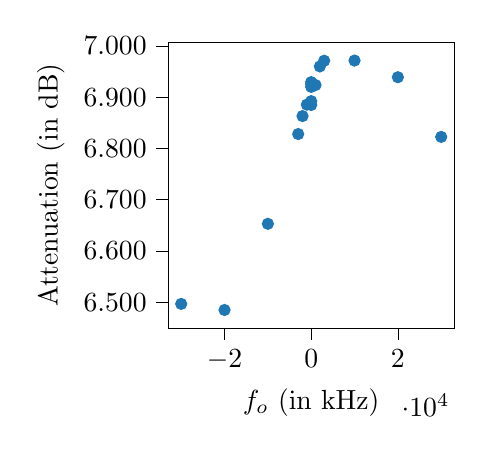
\begin{tikzpicture}[
baseline,
]

\definecolor{color0}{rgb}{0.12156862745098,0.466666666666667,0.705882352941177}

\begin{axis}[
height=0.43\textwidth,
ytick distance=0.1,
tick align=outside,
tick pos=left,
width=0.43\textwidth,
x grid style={white!69.0196078431373!black},
xlabel={$f_o$ (in \si{\kHz})},
xmin=-33000.0073466986, xmax=33000.0073466986,
xtick style={color=black},
y grid style={white!69.0196078431373!black},
ylabel style={align=center},
ylabel={Attenuation (in \si{\dB})},
ymin=6.44956234557695, ymax=7.00689920227556,
ytick style={color=black},
yticklabel pos=lower,
y tick label style={
        /pgf/number format/.cd,
            fixed,
            fixed zerofill,
            precision=3,
        /tikz/.cd
    }
]
\addplot [only marks, mark=*, draw=color0, fill=color0, colormap/viridis]
table{%
x                      y
-29999.9999999998 6.49704080362745
-20000 6.48517944823129
-9999.99999999979 6.65312661396739
-3000.00000000011 6.82805338711268
-1999.99999999978 6.86303896803419
-999.99999999989 6.88534599751244
-1.00000000013978 6.91995292566434
0 6.89215273989011
0 6.88470073226562
0 6.92509045190909
1.00000000013978 6.92927676035294
999.99999999989 6.92353152521008
1999.99999999978 6.95979922043103
3000.00000000011 6.97091072853147
9999.99999999979 6.97128209962121
20000 6.93879379212121
29999.9999999998 6.82251071210526
};
\end{axis}

\end{tikzpicture}
}
        \qquad
        \subfloat[$f_o=\SI{+-1}{\kHz}$]{% This file was created by tikzplotlib v0.9.5.
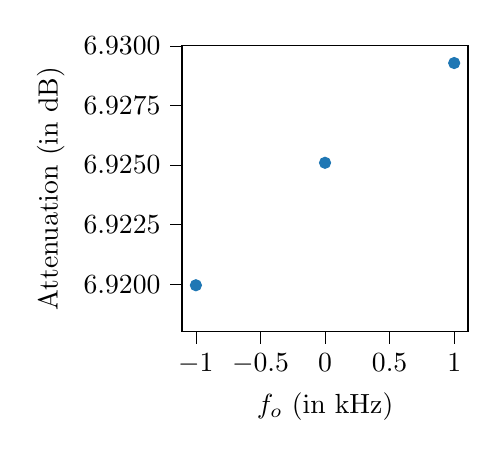
\begin{tikzpicture}[
baseline
]

\definecolor{color0}{rgb}{0.12156862745098,0.466666666666667,0.705882352941177}

\begin{axis}[
height=0.43\textwidth,
ytick distance=0.0025,
tick align=outside,
tick pos=left,
width=0.43\textwidth,
x grid style={white!69.0196078431373!black},
xlabel={$f_o$ (in \si{\kHz})},
xmin=-1.10734669900456, xmax=1.10734669900456,
xtick style={color=black},
y grid style={white!69.0196078431373!black},
ylabel style={align=center},
ylabel={Attenuation (in \si{\dB})},
ymin=6.918, ymax=6.93,
ytick style={color=black},
yticklabel pos=lower,
y tick label style={
        /pgf/number format/.cd,
            fixed,
            fixed zerofill,
            precision=4,
        /tikz/.cd
    }
]
\addplot [only marks, mark=*, draw=color0, fill=color0, colormap/viridis]
table{%
x                      y
-1.00000000013978 6.91995292566434
0 6.89215273989011
0 6.88470073226562
0 6.92509045190909
1.00000000013978 6.92927676035294
};
\end{axis}

\end{tikzpicture}
}
       \caption{Attenuation vs. offset frequency $f_o=f-\SI{3}{\GHz}$}
    \label{fig:atteneval-rf}
\end{figure}

\FloatBarrier
\section{Testing the Attenuator in the RF cabinet at FLUTE}
Without FLUTE being switched on, the attenuator is left in the RF cabinet in the bunker basement. Over the course of \SI{100}{\hour}, the case temperature is taken every two seconds and the deviation from the mean temperature \SI{25.4}{\degreeCelsius} is computed (see \autoref{fig:atteneval-tempInCabinet}). The figure also shows a power spectrum (calculated using Welch's method with a hanning window) of the temperature deviation.

With a standard deviation of \SI{0.05522}{\kelvin}, a maximum positive swing of \SI{0.18}{\kelvin} and a maximum negative swing of \SI{0.17}{\kelvin} (a span of \SI{0.3559}{\kelvin}), the temperature stability is well inside the \SI{0.6}{\kelvin} tolerance.

\begin{figure}[tb]
		\hfill
        \subfloat[Time]{% This file was created by tikzplotlib v0.9.5.
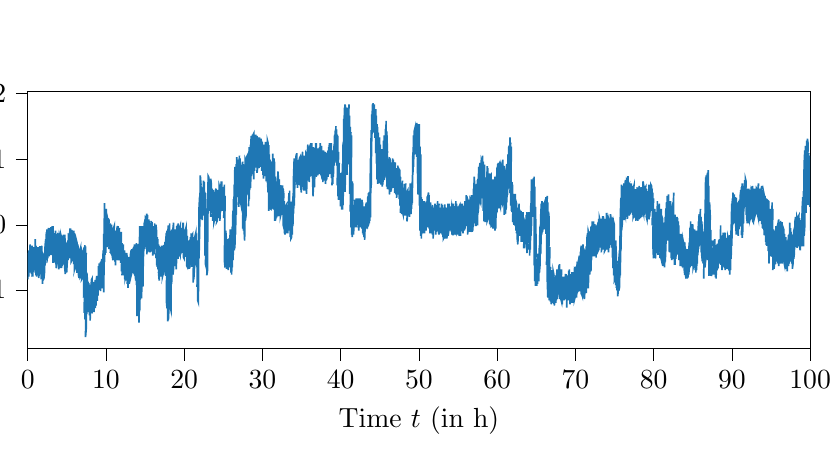
\begin{tikzpicture}[
baseline,
trim axis right,
trim axis left
]

\definecolor{color0}{rgb}{0.12156862745098,0.466666666666667,0.705882352941177}

\begin{axis}[
height=0.4\textwidth,
legend cell align={left},
legend style={fill opacity=0.8, draw opacity=1, text opacity=1, draw=white!80!black},
tick align=outside,
tick pos=left,
width=0.95\textwidth,
x grid style={white!69.0196078431373!black},
xlabel={Time \(\displaystyle t\) (in \si{\hour})},
xmin=0, xmax=100,
xtick style={color=black},
y grid style={white!69.0196078431373!black},
ylabel style={align=center},
ylabel={Temperature Deviation (in \si{\kelvin})},
ymin=-0.188649939113747, ymax=0.202950060886251,
ytick style={color=black},
yticklabel pos=lower
]
\addplot [semithick, color0]
table {%
0 -0.0828499391137463
0.0602777777777778 -0.0428499391137471
0.0608333333333333 -0.0728499391137483
0.143611111111111 -0.0388499391137493
0.144166666666667 -0.0788499391137485
0.227222222222222 -0.0388499391137493
0.227777777777778 -0.0678499391137493
0.310555555555556 -0.029849939113749
0.311388888888889 -0.0728499391137483
0.393611111111111 -0.0318499391137479
0.394166666666667 -0.0658499391137468
0.477222222222222 -0.0338499391137468
0.478055555555556 -0.0748499391137472
0.560277777777778 -0.0318499391137479
0.643611111111111 -0.0408499391137482
0.560833333333333 -0.0788499391137485
0.726944444444444 -0.0338499391137468
0.644166666666667 -0.0788499391137485
0.810277777777778 -0.0338499391137468
0.7275 -0.0658499391137468
0.893611111111111 -0.0338499391137468
0.810833333333333 -0.0658499391137468
0.894166666666667 -0.0678499391137493
0.977222222222222 -0.0218499391137463
0.978055555555556 -0.0728499391137483
1.06027777777778 -0.0318499391137479
1.06083333333333 -0.076849939113746
1.14361111111111 -0.0388499391137493
1.14416666666667 -0.0788499391137485
1.22694444444444 -0.0468499391137485
1.31027777777778 -0.0338499391137468
1.2275 -0.0728499391137483
1.31083333333333 -0.0728499391137483
1.39361111111111 -0.0338499391137468
1.47694444444444 -0.0408499391137482
1.39416666666667 -0.0808499391137474
1.4775 -0.0748499391137472
1.56027777777778 -0.0338499391137468
1.64388888888889 -0.0338499391137468
1.56083333333333 -0.0728499391137483
1.64472222222222 -0.0728499391137483
1.72722222222222 -0.0338499391137468
1.72777777777778 -0.0828499391137463
1.81055555555556 -0.0318499391137479
1.81111111111111 -0.0788499391137485
1.89361111111111 -0.0428499391137471
1.97694444444444 -0.044849939113746
1.89416666666667 -0.0898499391137477
2.06055555555556 -0.044849939113746
1.9775 -0.0848499391137487
2.14388888888889 -0.0468499391137485
2.06111111111111 -0.0828499391137463
2.14444444444444 -0.0728499391137483
2.22722222222222 -0.0318499391137479
2.31027777777778 -0.0218499391137463
2.22777777777778 -0.061849939113749
2.39361111111111 -0.0108499391137471
2.31083333333333 -0.0578499391137477
2.47694444444444 -0.00684993911374931
2.39416666666667 -0.044849939113746
2.4775 -0.0488499391137474
2.56027777777778 -0.00684993911374931
2.56083333333333 -0.0508499391137462
2.64361111111111 -0.00484993911374687
2.72722222222222 -0.0128499391137495
2.64416666666667 -0.0468499391137485
2.72777777777778 -0.0468499391137485
2.81055555555556 -0.00484993911374687
2.81111111111111 -0.0408499391137482
2.89361111111111 -0.00684993911374931
2.89444444444444 -0.044849939113746
2.97694444444444 -0.00484993911374687
3.06027777777778 -0.00484993911374687
2.9775 -0.044849939113746
3.06083333333333 -0.044849939113746
3.14361111111111 -0.00184993911374676
3.14416666666667 -0.0408499391137482
3.22694444444444 -0.00184993911374676
3.2275 -0.0578499391137477
3.31 -0.0168499391137473
3.31083333333333 -0.0578499391137477
3.39361111111111 -0.0218499391137463
3.47722222222222 -0.0128499391137495
3.39416666666667 -0.0488499391137474
3.56055555555556 -0.00884993911374821
3.47777777777778 -0.0508499391137462
3.56111111111111 -0.0558499391137488
3.64388888888889 -0.0188499391137462
3.72722222222222 -0.0168499391137473
3.64444444444444 -0.0658499391137468
3.72777777777778 -0.0578499391137477
3.81055555555556 -0.0188499391137462
3.81111111111111 -0.0538499391137464
3.89361111111111 -0.0148499391137484
3.89416666666667 -0.0558499391137488
3.97694444444444 -0.0128499391137495
3.9775 -0.0678499391137493
4.06027777777778 -0.0188499391137462
4.14361111111111 -0.0238499391137488
4.06083333333333 -0.0578499391137477
4.14416666666667 -0.0658499391137468
4.22722222222222 -0.0148499391137484
4.31 -0.0188499391137462
4.22777777777778 -0.0638499391137479
4.39388888888889 -0.0278499391137466
4.31083333333333 -0.0658499391137468
4.47722222222222 -0.0218499391137463
4.39444444444444 -0.0558499391137488
4.56027777777778 -0.0148499391137484
4.47777777777778 -0.0508499391137462
4.64361111111111 -0.0218499391137463
4.56083333333333 -0.0578499391137477
4.64444444444444 -0.0558499391137488
4.72722222222222 -0.0148499391137484
4.81055555555556 -0.029849939113749
4.72777777777778 -0.0638499391137479
4.81111111111111 -0.0748499391137472
4.89333333333333 -0.0388499391137493
4.89416666666667 -0.0658499391137468
4.97694444444444 -0.029849939113749
5.06027777777778 -0.0318499391137479
4.9775 -0.0728499391137483
5.06083333333333 -0.0558499391137488
5.14361111111111 -0.0238499391137488
5.14416666666667 -0.0538499391137464
5.22722222222222 -0.0128499391137495
5.22777777777778 -0.0488499391137474
5.31055555555556 -0.0168499391137473
5.31111111111111 -0.0508499391137462
5.39361111111111 -0.00684993911374931
5.47722222222222 -0.00684993911374931
5.39416666666667 -0.0428499391137471
5.47777777777778 -0.0488499391137474
5.56027777777778 -0.00884993911374821
5.64388888888889 -0.00884993911374821
5.56111111111111 -0.0558499391137488
5.64444444444444 -0.0538499391137464
5.72722222222222 -0.0168499391137473
5.72777777777778 -0.0508499391137462
5.81055555555556 -0.0148499391137484
5.81111111111111 -0.0488499391137474
5.89361111111111 -0.00884993911374821
5.89416666666667 -0.0598499391137466
5.97666666666667 -0.0128499391137495
6.06027777777778 -0.029849939113749
5.9775 -0.0678499391137493
6.06083333333333 -0.0638499391137479
6.14361111111111 -0.0258499391137477
6.14444444444444 -0.061849939113749
6.22722222222222 -0.0238499391137488
6.31055555555556 -0.0278499391137466
6.22777777777778 -0.0658499391137468
6.31111111111111 -0.0728499391137483
6.39388888888889 -0.029849939113749
6.47694444444444 -0.0368499391137469
6.39444444444444 -0.0728499391137483
6.56055555555556 -0.0388499391137493
6.4775 -0.0748499391137472
6.56111111111111 -0.0808499391137474
6.64388888888889 -0.0408499391137482
6.72722222222222 -0.0368499391137469
6.64444444444444 -0.076849939113746
6.81027777777778 -0.0388499391137493
6.72777777777778 -0.0788499391137485
6.81083333333333 -0.076849939113746
6.89361111111111 -0.0388499391137493
6.97722222222222 -0.0428499391137471
6.89444444444444 -0.0828499391137463
6.97777777777778 -0.0808499391137474
7.06027777777778 -0.0408499391137482
7.06083333333333 -0.0828499391137463
7.14361111111111 -0.0408499391137482
7.22694444444444 -0.0338499391137468
7.14416666666667 -0.110849939113749
7.31027777777778 -0.0308499391137467
7.2275 -0.133849939113748
7.39361111111111 -0.0328499391137491
7.31083333333333 -0.143849939113746
7.47694444444444 -0.0428499391137471
7.39416666666667 -0.170849939113747
7.4775 -0.158849939113747
7.56027777777778 -0.0728499391137483
7.64361111111111 -0.0868499391137476
7.56083333333333 -0.135849939113747
7.72694444444444 -0.0868499391137476
7.64416666666667 -0.129849939113747
7.81027777777778 -0.0888499391137465
7.7275 -0.132849939113747
7.89361111111111 -0.0908499391137489
7.81083333333333 -0.130849939113748
7.97694444444444 -0.0928499391137478
7.89416666666667 -0.13784993911375
8.06027777777778 -0.0928499391137478
7.9775 -0.145849939113749
8.06083333333333 -0.117849939113746
8.14361111111111 -0.0838499391137475
8.22694444444445 -0.0818499391137486
8.14416666666667 -0.124849939113748
8.31027777777778 -0.0928499391137478
8.2275 -0.134849939113749
8.31083333333333 -0.122849939113749
8.39361111111111 -0.0908499391137489
8.39416666666667 -0.128849939113749
8.47694444444445 -0.0868499391137476
8.4775 -0.132849939113747
8.56055555555556 -0.0908499391137489
8.56111111111111 -0.124849939113748
8.64361111111111 -0.0838499391137475
8.64416666666667 -0.126849939113747
8.72694444444445 -0.0908499391137489
8.7275 -0.122849939113749
8.81027777777778 -0.0778499391137473
8.81083333333333 -0.115849939113748
8.89361111111111 -0.0798499391137462
8.89416666666667 -0.115849939113748
8.97694444444445 -0.0798499391137462
8.9775 -0.107849939113748
9.06027777777778 -0.0628499391137467
9.06083333333333 -0.0948499391137467
9.14361111111111 -0.0588499391137489
9.14444444444444 -0.0988499391137481
9.22694444444445 -0.0588499391137489
9.2275 -0.0928499391137478
9.31027777777778 -0.0568499391137465
9.31083333333333 -0.100849939113747
9.39361111111111 -0.0548499391137476
9.39416666666667 -0.0968499391137492
9.47694444444445 -0.0518499391137475
9.4775 -0.0928499391137478
9.56055555555556 -0.0588499391137489
9.56111111111111 -0.0968499391137492
9.64388888888889 -0.0388499391137493
9.64444444444444 -0.0968499391137492
9.72722222222222 -0.0138499391137472
9.72777777777778 -0.102849939113749
9.81055555555556 0.0331500608862534
9.81111111111111 -0.0568499391137465
9.89361111111111 0.0181500608862528
9.89444444444444 -0.0458499391137472
9.97666666666667 0.0231500608862518
9.9775 -0.0428499391137471
10.0605555555556 0.024150060886253
10.0611111111111 -0.029849939113749
10.1438888888889 0.0131500608862538
10.2269444444444 0.00815006088625125
10.1444444444444 -0.0338499391137468
10.3105555555556 0.0101500608862537
10.2275 -0.0318499391137479
10.3938888888889 0.00815006088625125
10.3111111111111 -0.0318499391137479
10.4772222222222 0.000150060886252135
10.3947222222222 -0.0368499391137469
10.56 0.00215006088625103
10.4777777777778 -0.0368499391137469
10.6436111111111 -0.00184993911374676
10.5608333333333 -0.0428499391137471
10.7269444444444 0.000150060886252135
10.6441666666667 -0.0428499391137471
10.7275 -0.044849939113746
10.8105555555556 -0.00884993911374821
10.8936111111111 -0.00684993911374931
10.8111111111111 -0.0468499391137485
10.8941666666667 -0.0538499391137464
10.9769444444444 -0.00484993911374687
11.0602777777778 -0.00184993911374676
10.9775 -0.0468499391137485
11.0608333333333 -0.0468499391137485
11.1438888888889 -0.00884993911374821
11.1447222222222 -0.0558499391137488
11.2269444444444 -0.0188499391137462
11.2275 -0.061849939113749
11.3102777777778 -0.0168499391137473
11.3108333333333 -0.0538499391137464
11.3938888888889 -0.00684993911374931
11.4769444444444 -0.00184993911374676
11.3944444444444 -0.044849939113746
11.5602777777778 -0.00184993911374676
11.4775 -0.044849939113746
11.5608333333333 -0.0538499391137464
11.6436111111111 -0.0148499391137484
11.7269444444444 -0.00484993911374687
11.6441666666667 -0.0538499391137464
11.7275 -0.0468499391137485
11.81 -0.0108499391137471
11.8108333333333 -0.0508499391137462
11.8936111111111 -0.0218499391137463
11.9772222222222 -0.0108499391137471
11.8941666666667 -0.0578499391137477
12.0605555555556 -0.0278499391137466
11.9777777777778 -0.0708499391137494
12.1438888888889 -0.0338499391137468
12.0611111111111 -0.076849939113746
12.2272222222222 -0.029849939113749
12.1444444444444 -0.0728499391137483
12.3105555555556 -0.0408499391137482
12.2277777777778 -0.076849939113746
12.3936111111111 -0.0388499391137493
12.3111111111111 -0.0748499391137472
12.4772222222222 -0.0428499391137471
12.3941666666667 -0.0828499391137463
12.5605555555556 -0.0428499391137471
12.4777777777778 -0.0808499391137474
12.5611111111111 -0.076849939113746
12.6438888888889 -0.0428499391137471
12.7272222222222 -0.0508499391137462
12.6444444444444 -0.0848499391137487
12.8105555555556 -0.0538499391137464
12.7277777777778 -0.0898499391137477
12.8936111111111 -0.0488499391137474
12.8111111111111 -0.095849939113748
12.9772222222222 -0.0558499391137488
12.8941666666667 -0.0898499391137477
13.0605555555556 -0.0488499391137474
12.9777777777778 -0.0898499391137477
13.0611111111111 -0.0828499391137463
13.1438888888889 -0.044849939113746
13.2272222222222 -0.0388499391137493
13.1444444444444 -0.0808499391137474
13.3105555555556 -0.0368499391137469
13.2277777777778 -0.076849939113746
13.3111111111111 -0.0728499391137483
13.3936111111111 -0.0388499391137493
13.4772222222222 -0.0368499391137469
13.3941666666667 -0.0728499391137483
13.5602777777778 -0.0338499391137468
13.4777777777778 -0.0708499391137494
13.5608333333333 -0.0728499391137483
13.6436111111111 -0.029849939113749
13.6441666666667 -0.0658499391137468
13.7272222222222 -0.029849939113749
13.8102777777778 -0.0368499391137469
13.7277777777778 -0.0728499391137483
13.8108333333333 -0.0848499391137487
13.8933333333333 -0.0278499391137466
13.8941666666667 -0.0918499391137466
13.9769444444444 -0.029849939113749
13.9775 -0.138849939113747
14.0605555555556 -0.0318499391137479
14.0611111111111 -0.13784993911375
14.1438888888889 -0.0288499391137478
14.1444444444444 -0.121849939113748
14.2269444444444 -0.0308499391137467
14.2275 -0.148849939113749
14.3105555555556 -0.00184993911374676
14.3111111111111 -0.131849939113749
14.3938888888889 -0.00184993911374676
14.3944444444444 -0.113849939113749
14.4769444444444 -0.0178499391137485
14.4775 -0.0988499391137481
14.5602777777778 -0.0178499391137485
14.5608333333333 -0.111849939113746
14.6436111111111 -0.00184993911374676
14.6441666666667 -0.0898499391137477
14.7269444444444 -0.0108499391137471
14.7275 -0.0938499391137491
14.8105555555556 -0.0158499391137461
14.8111111111111 -0.0478499391137461
14.8938888888889 0.00315006088625225
14.8944444444444 -0.0338499391137468
14.9769444444444 0.00815006088625125
14.9775 -0.0368499391137469
15.0605555555556 0.0101500608862537
15.1438888888889 0.00815006088625125
15.0611111111111 -0.0258499391137477
15.2272222222222 0.0171500608862516
15.1444444444444 -0.0338499391137468
15.3102777777778 0.0151500608862527
15.2277777777778 -0.044849939113746
15.3936111111111 -0.00684993911374931
15.3108333333333 -0.0408499391137482
15.4769444444444 0.00815006088625125
15.3941666666667 -0.0388499391137493
15.5602777777778 0.00615006088625236
15.4775 -0.0368499391137469
15.6436111111111 0.00215006088625103
15.5608333333333 -0.0408499391137482
15.6441666666667 -0.0408499391137482
15.7269444444444 -0.00184993911374676
15.7275 -0.029849939113749
15.8102777777778 0.00615006088625236
15.8108333333333 -0.0408499391137482
15.8933333333333 0.00415006088625347
15.8941666666667 -0.0408499391137482
15.9766666666667 -0.00484993911374687
15.9775 -0.0468499391137485
16.0602777777778 -0.00184993911374676
16.0608333333333 -0.044849939113746
16.1436111111111 -0.00684993911374931
16.1441666666667 -0.044849939113746
16.2272222222222 0.00215006088625103
16.2277777777778 -0.0278499391137466
16.3102777777778 0.000150060886252135
16.3108333333333 -0.0368499391137469
16.3933333333333 0.000150060886252135
16.4772222222222 -0.0108499391137471
16.3941666666667 -0.0508499391137462
16.5602777777778 -0.0188499391137462
16.4777777777778 -0.061849939113749
16.6436111111111 -0.0218499391137463
16.5608333333333 -0.0638499391137479
16.7272222222222 -0.029849939113749
16.6441666666667 -0.0678499391137493
16.8105555555556 -0.0318499391137479
16.7277777777778 -0.0728499391137483
16.8111111111111 -0.0848499391137487
16.8938888888889 -0.0338499391137468
16.8944444444444 -0.0748499391137472
16.9766666666667 -0.0338499391137468
16.9775 -0.0788499391137485
17.0602777777778 -0.0388499391137493
17.1436111111111 -0.0318499391137479
17.0608333333333 -0.0748499391137472
17.2272222222222 -0.0338499391137468
17.1441666666667 -0.0748499391137472
17.3105555555556 -0.0388499391137493
17.2277777777778 -0.0788499391137485
17.3111111111111 -0.0748499391137472
17.3936111111111 -0.0318499391137479
17.4766666666667 -0.0318499391137479
17.3941666666667 -0.0708499391137494
17.4775 -0.061849939113749
17.5602777777778 -0.0258499391137477
17.5608333333333 -0.0758499391137484
17.6433333333333 -0.0238499391137488
17.7269444444444 -0.0118499391137483
17.6441666666667 -0.0778499391137473
17.8102777777778 -0.00884993911374821
17.7275 -0.115849939113748
17.8108333333333 -0.126849939113747
17.8936111111111 -0.0138499391137472
17.9772222222222 -0.000849939113749087
17.8941666666667 -0.146849939113746
18.0605555555556 -0.0158499391137461
17.9777777777778 -0.144849939113747
18.0611111111111 -0.124849939113748
18.1436111111111 0.00215006088625103
18.1441666666667 -0.111849939113746
18.2272222222222 -0.0138499391137472
18.3105555555556 -0.0118499391137483
18.2277777777778 -0.124849939113748
18.3111111111111 -0.129849939113747
18.3938888888889 -0.0108499391137471
18.4772222222222 -0.0118499391137483
18.3944444444444 -0.0898499391137477
18.4777777777778 -0.0588499391137489
18.5605555555556 -0.00684993911374931
18.6438888888889 0.00315006088625225
18.5611111111111 -0.0758499391137484
18.6444444444444 -0.066849939113748
18.7272222222222 -0.0148499391137484
18.8105555555556 -0.00684993911374931
18.7277777777778 -0.0628499391137467
18.8938888888889 -0.0108499391137471
18.8111111111111 -0.0608499391137478
18.9772222222222 -0.00984993911374943
18.8944444444444 -0.0538499391137464
19.0602777777778 -0.00184993911374676
18.9777777777778 -0.0678499391137493
19.0608333333333 -0.0438499391137483
19.1436111111111 0.000150060886252135
19.1441666666667 -0.0388499391137493
19.2269444444444 0.00215006088625103
19.2275 -0.0518499391137475
19.3102777777778 -0.00184993911374676
19.3108333333333 -0.0478499391137461
19.3938888888889 -0.00484993911374687
19.4772222222222 -0.00184993911374676
19.3944444444444 -0.0408499391137482
19.4777777777778 -0.044849939113746
19.5605555555556 -0.00684993911374931
19.5611111111111 -0.044849939113746
19.6438888888889 -0.00484993911374687
19.6444444444444 -0.0368499391137469
19.7272222222222 -0.00484993911374687
19.7277777777778 -0.0388499391137493
19.8102777777778 0.00215006088625103
19.8936111111111 0.00215006088625103
19.8108333333333 -0.0428499391137471
19.9769444444444 -0.0128499391137495
19.8941666666667 -0.0488499391137474
19.9775 -0.0508499391137462
20.0602777777778 -0.00684993911374931
20.0608333333333 -0.044849939113746
20.1436111111111 -0.00884993911374821
20.2272222222222 -0.00484993911374687
20.1441666666667 -0.044849939113746
20.3105555555556 -0.00684993911374931
20.2277777777778 -0.0488499391137474
20.3936111111111 -0.0168499391137473
20.3111111111111 -0.061849939113749
20.3941666666667 -0.0638499391137479
20.4769444444444 -0.0238499391137488
20.4775 -0.0638499391137479
20.5602777777778 -0.0278499391137466
20.6436111111111 -0.0258499391137477
20.5608333333333 -0.0658499391137468
20.6441666666667 -0.0658499391137468
20.7269444444444 -0.029849939113749
20.7275 -0.0658499391137468
20.8105555555556 -0.0188499391137462
20.8111111111111 -0.0598499391137466
20.8938888888889 -0.0128499391137495
20.8947222222222 -0.0578499391137477
20.9772222222222 -0.0168499391137473
21.06 -0.0148499391137484
20.9777777777778 -0.0638499391137479
21.1438888888889 -0.0218499391137463
21.0608333333333 -0.0598499391137466
21.2269444444444 -0.0188499391137462
21.1444444444444 -0.0878499391137488
21.3105555555556 -0.0388499391137493
21.2275 -0.0828499391137463
21.3111111111111 -0.0658499391137468
21.3936111111111 -0.0168499391137473
21.4769444444444 -0.0128499391137495
21.3941666666667 -0.0508499391137462
21.5602777777778 -0.0128499391137495
21.4775 -0.0558499391137488
21.5608333333333 -0.0598499391137466
21.6438888888889 -0.0238499391137488
21.7272222222222 -0.029849939113749
21.6444444444444 -0.0948499391137467
21.8105555555556 -0.0278499391137466
21.7277777777778 -0.114849939113746
21.8111111111111 -0.117849939113746
21.8938888888889 0.024150060886253
21.9769444444444 0.0431500608862514
21.8944444444444 -0.0508499391137462
21.9775 -0.00584993911374809
22.0602777777778 0.0751500608862514
22.1436111111111 0.0621500608862533
22.0608333333333 0.024150060886253
22.1444444444444 0.0181500608862528
22.2269444444444 0.0561500608862531
22.3105555555556 0.0541500608862506
22.2275 0.00915006088625248
22.3938888888889 0.0501500608862528
22.3111111111111 0.00715006088625358
22.4769444444444 0.0671500608862523
22.3947222222222 0.0181500608862528
22.4775 0.0181500608862528
22.5602777777778 0.0651500608862534
22.5608333333333 0.0141500608862515
22.6433333333333 0.0501500608862528
22.6441666666667 -0.0468499391137485
22.7272222222222 0.048150060886254
22.8102777777778 0.0111500608862514
22.7277777777778 -0.0598499391137466
22.8108333333333 -0.0638499391137479
22.8936111111111 -0.000849939113749087
22.9769444444444 0.0161500608862539
22.8941666666667 -0.076849939113746
22.9775 -0.0698499391137481
23.0605555555556 0.0741500608862538
23.1438888888889 0.0721500608862513
23.0611111111111 0.0171500608862516
23.2272222222222 0.0701500608862524
23.1444444444444 0.029150060886252
23.3105555555556 0.0681500608862535
23.2277777777778 0.029150060886252
23.3111111111111 0.0211500608862529
23.3938888888889 0.0701500608862524
23.4772222222222 0.0611500608862521
23.3944444444444 0.0121500608862526
23.5605555555556 0.0551500608862519
23.4777777777778 0.0191500608862505
23.6436111111111 0.0491500608862516
23.5611111111111 0.0191500608862505
23.7269444444444 0.053150060886253
23.6441666666667 0.00615006088625236
23.8105555555556 0.0461500608862515
23.7275 0.00815006088625125
23.8938888888889 0.0421500608862537
23.8111111111111 0.00415006088625347
23.8944444444444 0.00815006088625125
23.9772222222222 0.0491500608862516
24.0602777777778 0.0551500608862519
23.9777777777778 0.00815006088625125
24.1436111111111 0.0421500608862537
24.0611111111111 0.00615006088625236
24.2269444444444 0.053150060886253
24.1441666666667 0.00415006088625347
24.2275 0.00615006088625236
24.3102777777778 0.0511500608862505
24.3938888888889 0.0511500608862505
24.3108333333333 0.0101500608862537
24.3944444444444 0.0211500608862529
24.4772222222222 0.0591500608862532
24.5602777777778 0.0551500608862519
24.4780555555556 0.0151500608862527
24.6438888888889 0.0591500608862532
24.5611111111111 0.00615006088625236
24.7272222222222 0.0661500608862511
24.6444444444444 0.0191500608862505
24.8105555555556 0.0661500608862511
24.7277777777778 0.0251500608862507
24.8936111111111 0.0571500608862507
24.8111111111111 0.0211500608862529
24.9769444444444 0.0571500608862507
24.8941666666667 0.0211500608862529
25.0602777777778 0.0551500608862519
24.9775 0.0231500608862518
25.1436111111111 0.0611500608862521
25.0608333333333 0.0101500608862537
25.2269444444444 0.0441500608862526
25.1441666666667 -0.0548499391137476
25.2275 -0.0648499391137491
25.3102777777778 -0.00884993911374821
25.3938888888889 -0.0218499391137463
25.3108333333333 -0.0648499391137491
25.4772222222222 -0.0218499391137463
25.3944444444444 -0.066849939113748
25.5605555555556 -0.0238499391137488
25.4777777777778 -0.0628499391137467
25.6438888888889 -0.0238499391137488
25.5611111111111 -0.0608499391137478
25.6444444444444 -0.0688499391137469
25.7269444444444 -0.0218499391137463
25.8102777777778 -0.0218499391137463
25.7275 -0.0608499391137478
25.8936111111111 -0.00684993911374931
25.8108333333333 -0.0648499391137491
25.9772222222222 -0.0168499391137473
25.8941666666667 -0.0608499391137478
26.0605555555556 -0.0238499391137488
25.9777777777778 -0.0728499391137483
26.1438888888889 -0.00284993911374798
26.0611111111111 -0.0758499391137484
26.2272222222222 0.0211500608862529
26.1444444444444 -0.0648499391137491
26.3105555555556 0.0391500608862536
26.2277777777778 -0.0538499391137464
26.3111111111111 -0.0338499391137468
26.3938888888889 0.0611500608862521
26.3944444444444 -0.0388499391137493
26.4772222222222 0.0881500608862531
26.5605555555556 0.0731500608862525
26.4777777777778 -0.0358499391137492
26.6436111111111 0.0921500608862509
26.5611111111111 -0.0148499391137484
26.7269444444444 0.103150060886254
26.6441666666667 0.0151500608862527
26.8105555555556 0.0921500608862509
26.7275 0.0421500608862537
26.8938888888889 0.0961500608862522
26.8111111111111 0.0421500608862537
26.9772222222222 0.0991500608862523
26.8944444444444 0.0491500608862516
27.0605555555556 0.105150060886253
26.9777777777778 0.0271500608862532
27.1438888888889 0.101150060886251
27.0611111111111 0.0441500608862526
27.2269444444444 0.090150060886252
27.1444444444444 0.0451500608862538
27.3105555555556 0.0881500608862531
27.2275 0.0331500608862534
27.3111111111111 0.0281500608862508
27.3938888888889 0.090150060886252
27.4769444444444 0.0961500608862522
27.3944444444444 0.0221500608862506
27.5605555555556 0.0881500608862531
27.4775 -0.00584993911374809
27.6436111111111 0.0921500608862509
27.5611111111111 -0.00884993911374821
27.7269444444444 0.0881500608862531
27.6441666666667 -0.0038499391137492
27.7275 -0.0238499391137488
27.8105555555556 0.0991500608862523
27.8938888888889 0.0961500608862522
27.8111111111111 0.00615006088625236
27.8944444444444 0.0131500608862538
27.9769444444444 0.103150060886254
28.0605555555556 0.105150060886253
27.9775 0.053150060886253
28.1438888888889 0.103150060886254
28.0611111111111 0.0461500608862515
28.2269444444444 0.109150060886254
28.1444444444444 0.0501500608862528
28.3102777777778 0.118150060886251
28.2275 0.0281500608862508
28.3938888888889 0.118150060886251
28.3108333333333 0.0391500608862536
28.4772222222222 0.122150060886252
28.3944444444444 0.0541500608862506
28.5602777777778 0.135150060886254
28.4777777777778 0.0561500608862531
28.6438888888889 0.135150060886254
28.5608333333333 0.0741500608862538
28.6444444444444 0.0831500608862505
28.7272222222222 0.137150060886253
28.7280555555556 0.0891500608862508
28.8105555555556 0.137150060886253
28.8936111111111 0.139150060886251
28.8111111111111 0.0921500608862509
28.8941666666667 0.0691500608862512
28.9769444444444 0.137150060886253
28.9775 0.0821500608862529
29.0602777777778 0.133150060886251
29.0608333333333 0.0961500608862522
29.1436111111111 0.137150060886253
29.1441666666667 0.0871500608862519
29.2269444444444 0.135150060886254
29.2275 0.0961500608862522
29.3102777777778 0.135150060886254
29.3936111111111 0.128150060886252
29.3108333333333 0.0791500608862528
29.3941666666667 0.0881500608862531
29.4769444444444 0.126150060886253
29.4775 0.0941500608862533
29.5602777777778 0.133150060886251
29.5608333333333 0.0861500608862507
29.6436111111111 0.133150060886251
29.6441666666667 0.0921500608862509
29.7269444444444 0.131150060886252
29.7277777777778 0.0881500608862531
29.8102777777778 0.131150060886252
29.8111111111111 0.0881500608862531
29.8936111111111 0.128150060886252
29.8941666666667 0.0821500608862529
29.9772222222222 0.126150060886253
29.9777777777778 0.0841500608862518
30.0602777777778 0.122150060886252
30.0608333333333 0.0761500608862526
30.1436111111111 0.122150060886252
30.1441666666667 0.0701500608862524
30.2269444444444 0.122150060886252
30.2275 0.0771500608862539
30.3102777777778 0.120150060886253
30.3108333333333 0.080150060886254
30.3936111111111 0.126150060886253
30.3941666666667 0.0741500608862538
30.4769444444444 0.122150060886252
30.4775 0.0661500608862511
30.5602777777778 0.126150060886253
30.5608333333333 0.0731500608862525
30.6438888888889 0.128150060886252
30.7272222222222 0.124150060886251
30.6444444444444 0.0671500608862523
30.7277777777778 0.0491500608862516
30.8105555555556 0.121150060886251
30.8111111111111 0.0211500608862529
30.8938888888889 0.107150060886251
30.8944444444444 0.0271500608862532
30.9772222222222 0.0991500608862523
31.0605555555556 0.085150060886253
30.9777777777778 0.0251500608862507
31.0611111111111 0.024150060886253
31.1438888888889 0.0811500608862517
31.1444444444444 0.0251500608862507
31.2272222222222 0.0961500608862522
31.2277777777778 0.0251500608862507
31.3102777777778 0.108150060886253
31.3936111111111 0.090150060886252
31.3111111111111 0.0261500608862519
31.3941666666667 0.0271500608862532
31.4769444444444 0.101150060886251
31.4775 0.0231500608862518
31.5602777777778 0.0961500608862522
31.5608333333333 0.00615006088625236
31.6438888888889 0.0731500608862525
31.7272222222222 0.0611500608862521
31.6444444444444 0.00615006088625236
31.7277777777778 0.0111500608862514
31.8105555555556 0.0601500608862509
31.8113888888889 0.0111500608862514
31.8938888888889 0.0651500608862534
31.8944444444444 0.0131500608862538
31.9772222222222 0.0811500608862517
32.0605555555556 0.0671500608862523
31.9777777777778 0.0191500608862505
32.0611111111111 0.0131500608862538
32.1438888888889 0.0691500608862512
32.1444444444444 0.0131500608862538
32.2272222222222 0.0511500608862505
32.2277777777778 0.0131500608862538
32.3105555555556 0.053150060886253
32.3938888888889 0.0601500608862509
32.3111111111111 0.0131500608862538
32.3944444444444 0.0171500608862516
32.4772222222222 0.0551500608862519
32.4777777777778 0.0171500608862516
32.5605555555556 0.0601500608862509
32.5611111111111 0.0151500608862527
32.6436111111111 0.0551500608862519
32.7269444444444 0.0471500608862527
32.6441666666667 0.000150060886252135
32.7275 -0.0038499391137492
32.8102777777778 0.0361500608862535
32.8108333333333 -0.0128499391137495
32.8936111111111 0.0281500608862508
32.8941666666667 -0.0148499391137484
32.9769444444444 0.0281500608862508
33.0602777777778 0.0301500608862533
32.9775 -0.00584993911374809
33.0608333333333 -0.0038499391137492
33.1436111111111 0.0301500608862533
33.1441666666667 -0.0128499391137495
33.2272222222222 0.0261500608862519
33.2277777777778 -0.0128499391137495
33.3105555555556 0.0261500608862519
33.3938888888889 0.048150060886254
33.3111111111111 -0.0038499391137492
33.3944444444444 0.00215006088625103
33.4769444444444 0.0521500608862517
33.4775 -0.00884993911374821
33.5602777777778 0.0331500608862534
33.5608333333333 -0.0188499391137462
33.6438888888889 0.0351500608862523
33.7272222222222 0.0231500608862518
33.6444444444444 -0.0208499391137487
33.7277777777778 -0.0188499391137462
33.8105555555556 0.0201500608862517
33.8111111111111 -0.0148499391137484
33.8936111111111 0.0431500608862514
33.8941666666667 -0.00184993911374676
33.9769444444444 0.0721500608862513
34.0602777777778 0.101150060886251
33.9775 0.0171500608862516
34.1438888888889 0.101150060886251
34.0608333333333 0.029150060886252
34.2269444444444 0.101150060886251
34.1444444444444 0.0621500608862533
34.3102777777778 0.107150060886251
34.2275 0.0651500608862534
34.3936111111111 0.109150060886254
34.3108333333333 0.0651500608862534
34.4769444444444 0.0991500608862523
34.3941666666667 0.0611500608862521
34.5602777777778 0.0991500608862523
34.4775 0.0561500608862531
34.6436111111111 0.0991500608862523
34.5608333333333 0.0621500608862533
34.6441666666667 0.0621500608862533
34.7269444444444 0.101150060886251
34.8102777777778 0.103150060886254
34.7275 0.0651500608862534
34.8936111111111 0.0961500608862522
34.8108333333333 0.0601500608862509
34.9772222222222 0.105150060886253
34.8941666666667 0.058150060886252
34.9777777777778 0.0491500608862516
35.0605555555556 0.103150060886254
35.1433333333333 0.111150060886253
35.0611111111111 0.0611500608862521
35.2269444444444 0.105150060886253
35.1441666666667 0.063150060886251
35.3102777777778 0.105150060886253
35.2275 0.0611500608862521
35.3108333333333 0.0521500608862517
35.3936111111111 0.0961500608862522
35.4769444444444 0.103150060886254
35.3941666666667 0.0591500608862532
35.4775 0.0561500608862531
35.5602777777778 0.109150060886254
35.6436111111111 0.107150060886251
35.5608333333333 0.0711500608862536
35.6441666666667 0.0471500608862527
35.7269444444444 0.107150060886251
35.8105555555556 0.122150060886252
35.7275 0.0731500608862525
35.8111111111111 0.0711500608862536
35.8938888888889 0.113150060886252
35.9769444444444 0.116150060886252
35.8944444444444 0.0671500608862523
36.0602777777778 0.113150060886252
35.9775 0.0651500608862534
36.1436111111111 0.116150060886252
36.0608333333333 0.0731500608862525
36.2269444444444 0.124150060886251
36.1441666666667 0.0821500608862529
36.3105555555556 0.124150060886251
36.2275 0.0741500608862538
36.3938888888889 0.118150060886251
36.3111111111111 0.0741500608862538
36.4772222222222 0.118150060886251
36.3944444444444 0.0771500608862539
36.4780555555556 0.0431500608862514
36.5602777777778 0.116150060886252
36.6438888888889 0.116150060886252
36.5608333333333 0.0791500608862528
36.7272222222222 0.113150060886252
36.6444444444444 0.0571500608862507
36.8105555555556 0.124150060886251
36.7277777777778 0.0791500608862528
36.8938888888889 0.124150060886251
36.8111111111111 0.0821500608862529
36.9769444444444 0.113150060886252
36.8944444444444 0.0731500608862525
37.0602777777778 0.113150060886252
36.9775 0.0791500608862528
37.1436111111111 0.116150060886252
37.0608333333333 0.0751500608862514
37.2269444444444 0.111150060886253
37.1444444444444 0.0821500608862529
37.3102777777778 0.118150060886251
37.2275 0.0771500608862539
37.3936111111111 0.124150060886251
37.3108333333333 0.0791500608862528
37.4769444444444 0.118150060886251
37.3941666666667 0.0821500608862529
37.5605555555556 0.120150060886253
37.4775 0.0751500608862514
37.6438888888889 0.113150060886252
37.5613888888889 0.0751500608862514
37.6444444444444 0.0691500608862512
37.7272222222222 0.113150060886252
37.7277777777778 0.0651500608862534
37.8102777777778 0.113150060886252
37.8111111111111 0.0731500608862525
37.8938888888889 0.109150060886254
37.9769444444444 0.109150060886254
37.8944444444444 0.0671500608862523
38.0605555555556 0.111150060886253
37.9775 0.0671500608862523
38.1438888888889 0.109150060886254
38.0611111111111 0.0621500608862533
38.2272222222222 0.105150060886253
38.1444444444444 0.0671500608862523
38.3105555555556 0.109150060886254
38.2277777777778 0.0691500608862512
38.3938888888889 0.113150060886252
38.3111111111111 0.0751500608862514
38.4772222222222 0.118150060886251
38.3944444444444 0.0731500608862525
38.5605555555556 0.124150060886251
38.4777777777778 0.0841500608862518
38.6436111111111 0.120150060886253
38.5611111111111 0.0771500608862539
38.7269444444444 0.124150060886251
38.6441666666667 0.0841500608862518
38.8102777777778 0.124150060886251
38.7275 0.0861500608862507
38.8938888888889 0.113150060886252
38.8108333333333 0.0711500608862536
38.9772222222222 0.103150060886254
38.8944444444444 0.0601500608862509
39.0605555555556 0.111150060886253
38.9777777777778 0.0621500608862533
39.1438888888889 0.120150060886253
39.0611111111111 0.0731500608862525
39.2269444444444 0.137150060886253
39.1444444444444 0.090150060886252
39.3105555555556 0.143150060886253
39.2275 0.0941500608862533
39.3938888888889 0.150150060886251
39.3111111111111 0.106150060886254
39.4769444444444 0.145150060886252
39.3944444444444 0.107150060886251
39.5602777777778 0.137150060886253
39.4775 0.090150060886252
39.6438888888889 0.135150060886254
39.5608333333333 0.0601500608862509
39.7269444444444 0.111150060886253
39.6447222222222 0.0431500608862514
39.8102777777778 0.0941500608862533
39.7275 0.0381500608862524
39.8108333333333 0.0431500608862514
39.8936111111111 0.0791500608862528
39.8941666666667 0.0431500608862514
39.9769444444444 0.0791500608862528
39.9775 0.0281500608862508
40.0602777777778 0.0791500608862528
40.0608333333333 0.0281500608862508
40.1436111111111 0.0721500608862513
40.1441666666667 0.0231500608862518
40.2269444444444 0.0931500608862521
40.2275 0.0231500608862518
40.3105555555556 0.125150060886252
40.3111111111111 0.0301500608862533
40.3936111111111 0.161150060886253
40.3941666666667 0.0721500608862513
40.4769444444444 0.178150060886253
40.4775 0.0641500608862522
40.5605555555556 0.183150060886252
40.6438888888889 0.176150060886251
40.5611111111111 0.0501500608862528
40.7269444444444 0.178150060886253
40.6444444444444 0.0771500608862539
40.8102777777778 0.176150060886251
40.7275 0.0781500608862515
40.8936111111111 0.178150060886253
40.8108333333333 0.0761500608862526
40.9769444444444 0.174150060886252
40.8941666666667 0.119150060886252
41.0602777777778 0.183150060886252
40.9775 0.0991500608862523
41.1436111111111 0.166150060886253
41.0608333333333 0.0921500608862509
41.2269444444444 0.149150060886253
41.1441666666667 0.0471500608862527
41.3102777777778 0.141150060886254
41.2275 0.0201500608862517
41.3936111111111 0.136150060886251
41.3108333333333 -0.0038499391137492
41.4769444444444 0.0661500608862511
41.3941666666667 -0.0148499391137484
41.5602777777778 0.063150060886251
41.4775 -0.0188499391137462
41.6438888888889 0.0301500608862533
41.5608333333333 -0.0108499391137471
41.7272222222222 0.0231500608862518
41.6444444444444 -0.0148499391137484
41.8105555555556 0.0381500608862524
41.7277777777778 -0.0038499391137492
41.8938888888889 0.0381500608862524
41.8111111111111 -0.0038499391137492
41.9772222222222 0.0401500608862513
41.8944444444444 0.00215006088625103
42.0605555555556 0.0401500608862513
41.9777777777778 -0.0038499391137492
42.1436111111111 0.0361500608862535
42.0611111111111 -0.0038499391137492
42.2269444444444 0.0361500608862535
42.1441666666667 0.00215006088625103
42.3102777777778 0.0401500608862513
42.2275 0.00215006088625103
42.3936111111111 0.0381500608862524
42.3108333333333 -0.00884993911374821
42.4769444444444 0.0401500608862513
42.3941666666667 0.000150060886252135
42.5605555555556 0.0341500608862511
42.4775 -0.0038499391137492
42.6438888888889 0.0321500608862522
42.5611111111111 -0.0038499391137492
42.7272222222222 0.0381500608862524
42.6444444444444 0.000150060886252135
42.8105555555556 0.0341500608862511
42.7277777777778 -0.00584993911374809
42.8938888888889 0.0281500608862508
42.8113888888889 -0.0128499391137495
42.9772222222222 0.0281500608862508
42.8944444444444 -0.0148499391137484
43.0602777777778 0.0281500608862508
42.9777777777778 -0.0188499391137462
43.1436111111111 0.0281500608862508
43.0608333333333 -0.0228499391137476
43.2272222222222 0.0321500608862522
43.1441666666667 -0.00584993911374809
43.3102777777778 0.0341500608862511
43.2280555555556 -0.00584993911374809
43.3936111111111 0.0341500608862511
43.3108333333333 0.000150060886252135
43.4766666666667 0.0431500608862514
43.3941666666667 -0.00584993911374809
43.5602777777778 0.048150060886254
43.4775 -0.00184993911374676
43.5608333333333 0.000150060886252135
43.6436111111111 0.0501500608862528
43.6441666666667 0.00215006088625103
43.7269444444444 0.0501500608862528
43.7275 0.00615006088625236
43.8102777777778 0.101150060886251
43.8108333333333 0.0111500608862514
43.8938888888889 0.14415006088625
43.8944444444444 0.0561500608862531
43.9769444444444 0.168150060886251
43.9775 0.127150060886251
44.0602777777778 0.183150060886252
44.0608333333333 0.140150060886253
44.1436111111111 0.185150060886251
44.1441666666667 0.14415006088625
44.2269444444444 0.181150060886253
44.2275 0.142150060886252
44.3102777777778 0.183150060886252
44.3108333333333 0.140150060886253
44.3936111111111 0.176150060886251
44.3941666666667 0.132150060886254
44.4769444444444 0.176150060886251
44.4775 0.109150060886254
44.5602777777778 0.166150060886253
44.5608333333333 0.0931500608862521
44.6436111111111 0.153150060886251
44.6441666666667 0.0691500608862512
44.7272222222222 0.149150060886253
44.7277777777778 0.0621500608862533
44.8105555555556 0.140150060886253
44.8111111111111 0.063150060886251
44.8938888888889 0.122150060886252
44.8944444444444 0.063150060886251
44.9772222222222 0.133150060886251
44.9777777777778 0.0651500608862534
45.0605555555556 0.122150060886252
45.0611111111111 0.0681500608862535
45.1438888888889 0.115150060886251
45.1444444444444 0.0611500608862521
45.2272222222222 0.115150060886251
45.2277777777778 0.0611500608862521
45.3105555555556 0.113150060886252
45.3111111111111 0.058150060886252
45.3933333333333 0.113150060886252
45.3941666666667 0.0611500608862521
45.4772222222222 0.128150060886252
45.4777777777778 0.0691500608862512
45.5602777777778 0.136150060886251
45.5608333333333 0.0681500608862535
45.6438888888889 0.136150060886251
45.6444444444444 0.0711500608862536
45.7272222222222 0.146150060886253
45.7277777777778 0.0891500608862508
45.8102777777778 0.158150060886253
45.8108333333333 0.0731500608862525
45.8938888888889 0.142150060886252
45.9772222222222 0.111150060886253
45.8944444444444 0.058150060886252
46.0605555555556 0.0881500608862531
45.9777777777778 0.0541500608862506
46.1438888888889 0.090150060886252
46.0611111111111 0.0561500608862531
46.2272222222222 0.103150060886254
46.1444444444444 0.0541500608862506
46.31 0.101150060886251
46.2277777777778 0.0461500608862515
46.3936111111111 0.095150060886251
46.3108333333333 0.058150060886252
46.4769444444444 0.090150060886252
46.3941666666667 0.0501500608862528
46.5605555555556 0.090150060886252
46.4775 0.0521500608862517
46.6438888888889 0.101150060886251
46.5611111111111 0.058150060886252
46.7272222222222 0.0991500608862523
46.6444444444444 0.0561500608862531
46.8102777777778 0.0931500608862521
46.7277777777778 0.063150060886251
46.8936111111111 0.0931500608862521
46.8108333333333 0.0561500608862531
46.9769444444444 0.095150060886251
46.8941666666667 0.048150060886254
47.0602777777778 0.0861500608862507
46.9775 0.048150060886254
47.1438888888889 0.080150060886254
47.0608333333333 0.0461500608862515
47.2272222222222 0.0861500608862507
47.1444444444444 0.0411500608862525
47.2277777777778 0.0501500608862528
47.3105555555556 0.090150060886252
47.3111111111111 0.0461500608862515
47.3938888888889 0.0861500608862507
47.4772222222222 0.0841500608862518
47.3944444444444 0.0461500608862515
47.5605555555556 0.0841500608862518
47.4777777777778 0.0391500608862536
47.6436111111111 0.0731500608862525
47.5611111111111 0.029150060886252
47.7269444444444 0.0641500608862522
47.6444444444444 0.0181500608862528
47.8102777777778 0.063150060886251
47.7275 0.0201500608862517
47.8938888888889 0.0671500608862523
47.8111111111111 0.0161500608862539
47.9766666666667 0.0561500608862531
47.8944444444444 0.0201500608862517
47.9775 0.0161500608862539
48.06 0.0561500608862531
48.0608333333333 0.0141500608862515
48.1438888888889 0.0611500608862521
48.2272222222222 0.0611500608862521
48.1444444444444 0.0271500608862532
48.3105555555556 0.063150060886251
48.2277777777778 0.024150060886253
48.3111111111111 0.0141500608862515
48.3938888888889 0.0521500608862517
48.3944444444444 0.0141500608862515
48.4772222222222 0.0501500608862528
48.5602777777778 0.0521500608862517
48.4777777777778 0.00515006088625114
48.5608333333333 0.0161500608862539
48.6436111111111 0.0521500608862517
48.6441666666667 0.0161500608862539
48.7269444444444 0.048150060886254
48.7275 0.0141500608862515
48.8102777777778 0.0501500608862528
48.8108333333333 0.0121500608862526
48.8938888888889 0.063150060886251
48.8944444444444 0.0221500608862506
48.9772222222222 0.0561500608862531
48.9777777777778 0.0161500608862539
49.0605555555556 0.0611500608862521
49.0611111111111 0.024150060886253
49.1438888888889 0.0651500608862534
49.1444444444444 0.0331500608862534
49.2272222222222 0.110150060886252
49.2277777777778 0.0761500608862526
49.3105555555556 0.136150060886251
49.3111111111111 0.0881500608862531
49.3938888888889 0.142150060886252
49.4772222222222 0.146150060886253
49.3944444444444 0.108150060886253
49.4777777777778 0.108150060886253
49.5602777777778 0.151150060886252
49.6436111111111 0.140150060886253
49.5608333333333 0.108150060886253
49.7269444444444 0.155150060886253
49.6441666666667 0.11215006088625
49.8105555555556 0.149150060886253
49.7275 0.103150060886254
49.8938888888889 0.153150060886251
49.8111111111111 0.0871500608862519
49.8944444444444 0.0461500608862515
49.9772222222222 0.14415006088625
49.9777777777778 0.0491500608862516
50.0605555555556 0.153150060886251
50.0611111111111 0.029150060886252
50.1438888888889 0.119150060886252
50.1444444444444 -0.00884993911374821
50.2272222222222 0.107150060886251
50.2277777777778 -0.0168499391137473
50.3105555555556 0.0421500608862537
50.3111111111111 -0.0208499391137487
50.3938888888889 0.0391500608862536
50.3944444444444 -0.0128499391137495
50.4772222222222 0.0221500608862506
50.4777777777778 -0.0108499391137471
50.5605555555556 0.0281500608862508
50.5611111111111 -0.00884993911374821
50.6438888888889 0.0361500608862535
50.6444444444444 -0.0128499391137495
50.7272222222222 0.0361500608862535
50.7277777777778 -0.0128499391137495
50.8102777777778 0.0341500608862511
50.8108333333333 -0.00584993911374809
50.8938888888889 0.0301500608862533
50.8944444444444 -0.00884993911374821
50.9769444444444 0.0321500608862522
50.9775 0.00815006088625125
51.0602777777778 0.0431500608862514
51.0608333333333 0.000150060886252135
51.1436111111111 0.0431500608862514
51.2269444444444 0.0491500608862516
51.1441666666667 -0.0038499391137492
51.3102777777778 0.0451500608862538
51.2275 -0.00184993911374676
51.3936111111111 0.0341500608862511
51.3108333333333 -0.00584993911374809
51.4769444444444 0.0341500608862511
51.3941666666667 -0.0128499391137495
51.5602777777778 0.0281500608862508
51.4775 -0.0108499391137471
51.6436111111111 0.0261500608862519
51.5608333333333 -0.0128499391137495
51.7269444444444 0.0301500608862533
51.6441666666667 -0.0108499391137471
51.8105555555556 0.0151500608862527
51.7275 -0.0148499391137484
51.8938888888889 0.0191500608862505
51.8111111111111 -0.0208499391137487
51.9772222222222 0.0281500608862508
51.8944444444444 -0.00884993911374821
52.0602777777778 0.0321500608862522
51.9780555555556 -0.0038499391137492
52.1436111111111 0.0301500608862533
52.0608333333333 -0.00884993911374821
52.2269444444444 0.0261500608862519
52.1441666666667 -0.0148499391137484
52.3105555555556 0.0261500608862519
52.2275 -0.0108499391137471
52.3936111111111 0.0361500608862535
52.3111111111111 -0.00584993911374809
52.4769444444444 0.0281500608862508
52.3941666666667 -0.00884993911374821
52.5602777777778 0.0321500608862522
52.4775 -0.00884993911374821
52.5608333333333 -0.0148499391137484
52.6438888888889 0.0261500608862519
52.6444444444444 -0.0128499391137495
52.7272222222222 0.0231500608862518
52.7277777777778 -0.0128499391137495
52.8105555555556 0.0231500608862518
52.8111111111111 -0.0038499391137492
52.8938888888889 0.0321500608862522
52.8944444444444 -0.0108499391137471
52.9772222222222 0.0301500608862533
52.9777777777778 -0.0148499391137484
53.0605555555556 0.0261500608862519
53.0611111111111 -0.0188499391137462
53.1438888888889 0.0191500608862505
53.2269444444444 0.0171500608862516
53.1444444444444 -0.0208499391137487
53.2275 -0.0188499391137462
53.3102777777778 0.0311500608862509
53.3111111111111 -0.0188499391137462
53.3938888888889 0.0151500608862527
53.3944444444444 -0.0208499391137487
53.4772222222222 0.0211500608862529
53.5605555555556 0.0261500608862519
53.4777777777778 -0.0168499391137473
53.6436111111111 0.0231500608862518
53.5611111111111 -0.0208499391137487
53.6441666666667 -0.0128499391137495
53.7266666666667 0.0321500608862522
53.8105555555556 0.0231500608862518
53.7275 -0.0168499391137473
53.8111111111111 -0.00884993911374821
53.8936111111111 0.0321500608862522
53.8941666666667 -0.0038499391137492
53.9772222222222 0.0281500608862508
53.9777777777778 -0.00884993911374821
54.06 0.0281500608862508
54.0608333333333 -0.00584993911374809
54.1436111111111 0.0281500608862508
54.1441666666667 -0.0108499391137471
54.2269444444444 0.0281500608862508
54.3105555555556 0.0231500608862518
54.2275 -0.0148499391137484
54.3938888888889 0.0321500608862522
54.3111111111111 -0.0148499391137484
54.3944444444444 -0.0148499391137484
54.4772222222222 0.0281500608862508
54.5605555555556 0.0191500608862505
54.4780555555556 -0.0148499391137484
54.6436111111111 0.0281500608862508
54.5611111111111 -0.0148499391137484
54.7269444444444 0.0361500608862535
54.6441666666667 -0.0108499391137471
54.7275 -0.0128499391137495
54.8102777777778 0.0321500608862522
54.8108333333333 -0.0148499391137484
54.8936111111111 0.0281500608862508
54.8941666666667 -0.0108499391137471
54.9769444444444 0.0261500608862519
54.9775 -0.0148499391137484
55.0605555555556 0.0231500608862518
55.0611111111111 -0.00584993911374809
55.1438888888889 0.0281500608862508
55.2272222222222 0.0301500608862533
55.1444444444444 -0.0168499391137473
55.2277777777778 -0.0108499391137471
55.3102777777778 0.0281500608862508
55.3936111111111 0.0261500608862519
55.3108333333333 -0.0168499391137473
55.4772222222222 0.0321500608862522
55.3941666666667 -0.00884993911374821
55.5605555555556 0.0321500608862522
55.4777777777778 -0.00884993911374821
55.6438888888889 0.0231500608862518
55.5611111111111 -0.00584993911374809
55.6444444444444 -0.0128499391137495
55.7269444444444 0.0261500608862519
55.8102777777778 0.0281500608862508
55.7275 -0.00884993911374821
55.8936111111111 0.0361500608862535
55.8108333333333 -0.00884993911374821
55.9769444444444 0.0341500608862511
55.8941666666667 -0.00584993911374809
56.0602777777778 0.0451500608862538
55.9775 0.00215006088625103
56.0608333333333 0.00415006088625347
56.1436111111111 0.0431500608862514
56.1441666666667 -0.00184993911374676
56.2269444444444 0.0401500608862513
56.2275 -0.0148499391137484
56.3105555555556 0.0381500608862524
56.3938888888889 0.0321500608862522
56.3111111111111 -0.00884993911374821
56.3944444444444 -0.0038499391137492
56.4772222222222 0.0331500608862534
56.4777777777778 -0.0108499391137471
56.5605555555556 0.0381500608862524
56.6438888888889 0.0351500608862523
56.5611111111111 -0.0108499391137471
56.7272222222222 0.0451500608862538
56.6444444444444 -0.0108499391137471
56.7277777777778 -0.0038499391137492
56.8105555555556 0.0391500608862536
56.8111111111111 -0.0108499391137471
56.8936111111111 0.0411500608862525
56.8941666666667 -0.00884993911374821
56.9772222222222 0.0551500608862519
56.9780555555556 0.00415006088625347
57.0605555555556 0.0731500608862525
57.1438888888889 0.058150060886252
57.0611111111111 0.00215006088625103
57.1444444444444 0.00815006088625125
57.2272222222222 0.0561500608862531
57.2277777777778 -0.00184993911374676
57.3105555555556 0.0551500608862519
57.3111111111111 -0.00184993911374676
57.3938888888889 0.0621500608862533
57.3944444444444 0.00415006088625347
57.4766666666667 0.0671500608862523
57.56 0.0691500608862512
57.4775 -0.000849939113749087
57.6438888888889 0.0881500608862531
57.5608333333333 0.0181500608862528
57.6444444444444 0.0311500608862509
57.7272222222222 0.0861500608862507
57.8105555555556 0.0941500608862533
57.7277777777778 0.0471500608862527
57.8936111111111 0.0881500608862531
57.8111111111111 0.0361500608862535
57.8941666666667 0.0331500608862534
57.9769444444444 0.0991500608862523
58.0602777777778 0.0961500608862522
57.9775 0.0401500608862513
58.0608333333333 0.0641500608862522
58.1438888888889 0.105150060886253
58.1444444444444 0.0411500608862525
58.2272222222222 0.0961500608862522
58.2277777777778 0.0211500608862529
58.3102777777778 0.090150060886252
58.3936111111111 0.090150060886252
58.3108333333333 0.00515006088625114
58.4769444444444 0.0721500608862513
58.3941666666667 0.0151500608862527
58.5605555555556 0.0721500608862513
58.4777777777778 0.00415006088625347
58.6436111111111 0.0671500608862523
58.5611111111111 0.00615006088625236
58.7269444444444 0.0891500608862508
58.6441666666667 0.0121500608862526
58.8102777777778 0.0861500608862507
58.7275 0.00615006088625236
58.8111111111111 0.00915006088625248
58.8938888888889 0.0771500608862539
58.8944444444444 0.0211500608862529
58.9772222222222 0.0781500608862515
58.9777777777778 0.0141500608862515
59.0605555555556 0.0761500608862526
59.0611111111111 0.00115006088625336
59.1436111111111 0.0761500608862526
59.2269444444444 0.0771500608862539
59.1441666666667 -0.000849939113749087
59.3102777777778 0.0691500608862512
59.2277777777778 -0.00184993911374676
59.3108333333333 -0.000849939113749087
59.3936111111111 0.0621500608862533
59.3941666666667 -0.0038499391137492
59.4769444444444 0.0601500608862509
59.4775 -0.00584993911374809
59.5602777777778 0.0691500608862512
59.5608333333333 -0.00284993911374798
59.6438888888889 0.0511500608862505
59.6444444444444 -0.00584993911374809
59.7272222222222 0.0731500608862525
59.7277777777778 -0.00884993911374821
59.8105555555556 0.0521500608862517
59.8938888888889 0.0691500608862512
59.8111111111111 -0.00584993911374809
59.9769444444444 0.0871500608862519
59.8944444444444 0.0161500608862539
60.0602777777778 0.0921500608862509
59.9775 0.0191500608862505
60.0611111111111 0.0381500608862524
60.1436111111111 0.0941500608862533
60.1441666666667 0.0361500608862535
60.2269444444444 0.0921500608862509
60.3105555555556 0.0941500608862533
60.2275 0.0251500608862507
60.3938888888889 0.0961500608862522
60.3111111111111 0.0321500608862522
60.3947222222222 0.0281500608862508
60.4772222222222 0.0921500608862509
60.5602777777778 0.0921500608862509
60.4777777777778 0.0301500608862533
60.5608333333333 0.0391500608862536
60.6438888888889 0.0921500608862509
60.7272222222222 0.0991500608862523
60.6444444444444 0.0401500608862513
60.8105555555556 0.090150060886252
60.7280555555556 0.0331500608862534
60.8111111111111 0.0361500608862535
60.8938888888889 0.0891500608862508
60.8944444444444 0.0151500608862527
60.9772222222222 0.0821500608862529
60.9777777777778 0.0161500608862539
61.0605555555556 0.0841500608862518
61.0611111111111 0.0171500608862516
61.1438888888889 0.0841500608862518
61.2272222222222 0.0921500608862509
61.1444444444444 0.0231500608862518
61.3102777777778 0.090150060886252
61.2280555555556 0.0341500608862511
61.3936111111111 0.107150060886251
61.3108333333333 0.0451500608862538
61.3941666666667 0.0671500608862523
61.4769444444444 0.118150060886251
61.5605555555556 0.120150060886253
61.4775 0.0551500608862519
61.6438888888889 0.133150060886251
61.5611111111111 0.0621500608862533
61.7272222222222 0.125150060886252
61.6444444444444 0.048150060886254
61.8105555555556 0.119150060886252
61.7277777777778 0.029150060886252
61.8936111111111 0.0651500608862534
61.8111111111111 0.0211500608862529
61.9772222222222 0.0611500608862521
61.8941666666667 0.0191500608862505
62.0605555555556 0.0471500608862527
61.9777777777778 0.00415006088625347
62.1438888888889 0.0471500608862527
62.0611111111111 0.00815006088625125
62.1447222222222 0.000150060886252135
62.2269444444444 0.0451500608862538
62.2275 0.00215006088625103
62.31 0.0471500608862527
62.3108333333333 -0.00184993911374676
62.3938888888889 0.0361500608862535
62.4769444444444 0.0321500608862522
62.3944444444444 -0.00884993911374821
62.5605555555556 0.0261500608862519
62.4775 -0.0128499391137495
62.6438888888889 0.0211500608862529
62.5611111111111 -0.0208499391137487
62.6444444444444 -0.029849939113749
62.7266666666667 0.0191500608862505
62.8102777777778 0.0321500608862522
62.7275 -0.0128499391137495
62.8936111111111 0.0231500608862518
62.8108333333333 -0.0148499391137484
62.9769444444444 0.0191500608862505
62.8941666666667 -0.0168499391137473
63.0605555555556 0.0211500608862529
62.9775 -0.0168499391137473
63.1436111111111 0.0171500608862516
63.0611111111111 -0.0258499391137477
63.2269444444444 0.0171500608862516
63.1441666666667 -0.0258499391137477
63.3105555555556 0.0191500608862505
63.2275 -0.0258499391137477
63.3938888888889 0.0111500608862514
63.3111111111111 -0.0228499391137476
63.4766666666667 0.00415006088625347
63.3944444444444 -0.0358499391137492
63.5602777777778 0.00815006088625125
63.4775 -0.0358499391137492
63.6438888888889 0.00815006088625125
63.5608333333333 -0.029849939113749
63.7269444444444 0.0151500608862527
63.6444444444444 -0.0208499391137487
63.8102777777778 0.0191500608862505
63.7275 -0.0208499391137487
63.8108333333333 -0.0428499391137471
63.8938888888889 0.0111500608862514
63.9772222222222 0.0171500608862516
63.8944444444444 -0.0208499391137487
64.0605555555556 0.0191500608862505
63.9777777777778 -0.0278499391137466
64.1438888888889 0.00215006088625103
64.0611111111111 -0.0378499391137481
64.2269444444444 0.00415006088625347
64.1444444444444 -0.0468499391137485
64.3105555555556 0.0331500608862534
64.2275 -0.0378499391137481
64.3936111111111 0.0691500608862512
64.3111111111111 -0.0168499391137473
64.3941666666667 0.00215006088625103
64.4766666666667 0.0691500608862512
64.4775 0.0281500608862508
64.5602777777778 0.0601500608862509
64.5608333333333 0.0161500608862539
64.6436111111111 0.0711500608862536
64.6441666666667 0.0121500608862526
64.7269444444444 0.0731500608862525
64.7275 -0.061849939113749
64.8102777777778 0.058150060886252
64.8108333333333 -0.0858499391137464
64.8936111111111 0.0271500608862532
64.9769444444444 -0.0308499391137467
64.8941666666667 -0.0928499391137478
65.0602777777778 -0.0538499391137464
64.9775 -0.0858499391137464
65.1436111111111 -0.0518499391137475
65.0608333333333 -0.0928499391137478
65.2269444444444 -0.0438499391137483
65.1441666666667 -0.0898499391137477
65.3105555555556 -0.0438499391137483
65.2275 -0.0838499391137475
65.3938888888889 -0.0338499391137468
65.3111111111111 -0.0858499391137464
65.4772222222222 -0.00284993911374798
65.3944444444444 -0.0728499391137483
65.4777777777778 -0.0608499391137478
65.5602777777778 0.0111500608862514
65.6438888888889 0.0321500608862522
65.5611111111111 -0.0438499391137483
65.7272222222222 0.0361500608862535
65.6444444444444 -0.0158499391137461
65.7277777777778 -0.0108499391137471
65.81 0.0341500608862511
65.8108333333333 -0.0108499391137471
65.8938888888889 0.0341500608862511
65.8944444444444 -0.00484993911374687
65.9769444444444 0.0321500608862522
65.9775 -0.00484993911374687
66.0602777777778 0.029150060886252
66.1436111111111 0.0381500608862524
66.0608333333333 -0.00684993911374931
66.2269444444444 0.0421500608862537
66.1444444444444 0.00815006088625125
66.3102777777778 0.0401500608862513
66.2275 -0.0138499391137472
66.3938888888889 0.0441500608862526
66.3108333333333 -0.0608499391137478
66.4769444444444 0.0341500608862511
66.3944444444444 -0.0808499391137474
66.4775 -0.110849939113749
66.5602777777778 0.0201500608862517
66.6436111111111 0.00915006088625248
66.5608333333333 -0.10584993911375
66.7272222222222 -0.0338499391137468
66.6441666666667 -0.114849939113746
66.8105555555556 -0.0638499391137479
66.7277777777778 -0.114849939113746
66.8938888888889 -0.0688499391137469
66.8111111111111 -0.116849939113749
66.9772222222222 -0.0808499391137474
66.8944444444444 -0.120849939113747
67.0605555555556 -0.0748499391137472
66.9777777777778 -0.118849939113748
67.0611111111111 -0.110849939113749
67.1438888888889 -0.0698499391137481
67.2272222222222 -0.0748499391137472
67.1447222222222 -0.112849939113747
67.3102777777778 -0.0808499391137474
67.2280555555556 -0.120849939113747
67.3936111111111 -0.0788499391137485
67.3108333333333 -0.122849939113749
67.4772222222222 -0.076849939113746
67.3941666666667 -0.116849939113749
67.5605555555556 -0.076849939113746
67.4780555555556 -0.118849939113748
67.6436111111111 -0.0678499391137493
67.5611111111111 -0.114849939113746
67.7269444444444 -0.0678499391137493
67.6441666666667 -0.112849939113747
67.8102777777778 -0.0678499391137493
67.7275 -0.103849939113747
67.8936111111111 -0.061849939113749
67.8108333333333 -0.0998499391137493
67.9769444444444 -0.0598499391137466
67.8941666666667 -0.103849939113747
67.9775 -0.112849939113747
68.0602777777778 -0.0698499391137481
68.0608333333333 -0.108849939113746
68.1436111111111 -0.0748499391137472
68.2269444444444 -0.0678499391137493
68.1441666666667 -0.112849939113747
68.2275 -0.116849939113749
68.3105555555556 -0.0788499391137485
68.3111111111111 -0.120849939113747
68.3938888888889 -0.0808499391137474
68.3944444444444 -0.114849939113746
68.4772222222222 -0.0788499391137485
68.4777777777778 -0.114849939113746
68.5605555555556 -0.0808499391137474
68.5611111111111 -0.114849939113746
68.6438888888889 -0.0788499391137485
68.6444444444444 -0.112849939113747
68.7272222222222 -0.0748499391137472
68.7277777777778 -0.112849939113747
68.8105555555556 -0.0748499391137472
68.8111111111111 -0.112849939113747
68.8938888888889 -0.076849939113746
68.8944444444444 -0.125849939113749
68.9772222222222 -0.076849939113746
68.9777777777778 -0.114849939113746
69.0605555555556 -0.0808499391137474
69.0611111111111 -0.114849939113746
69.1438888888889 -0.0698499391137481
69.1444444444444 -0.114849939113746
69.2272222222222 -0.0678499391137493
69.2277777777778 -0.114849939113746
69.3105555555556 -0.0748499391137472
69.3111111111111 -0.120849939113747
69.3938888888889 -0.0808499391137474
69.4772222222222 -0.0788499391137485
69.3944444444444 -0.114849939113746
69.4777777777778 -0.108849939113746
69.5605555555556 -0.071849939113747
69.5611111111111 -0.118849939113748
69.6438888888889 -0.0808499391137474
69.7272222222222 -0.0808499391137474
69.6444444444444 -0.118849939113748
69.8105555555556 -0.071849939113747
69.7277777777778 -0.114849939113746
69.8113888888889 -0.10584993911375
69.8938888888889 -0.0658499391137468
69.9772222222222 -0.066849939113748
69.8944444444444 -0.112849939113747
69.9777777777778 -0.108849939113746
70.0605555555556 -0.0648499391137491
70.1438888888889 -0.0638499391137479
70.0611111111111 -0.110849939113749
70.2272222222222 -0.0558499391137488
70.1444444444444 -0.110849939113749
70.3105555555556 -0.0568499391137465
70.2277777777778 -0.103849939113747
70.3938888888889 -0.0528499391137487
70.3111111111111 -0.101849939113748
70.4766666666667 -0.0468499391137485
70.3944444444444 -0.095849939113748
70.5605555555556 -0.0478499391137461
70.4775 -0.0998499391137493
70.5613888888889 -0.0998499391137493
70.6438888888889 -0.0408499391137482
70.6444444444444 -0.095849939113748
70.7269444444444 -0.0318499391137479
70.8105555555556 -0.0518499391137475
70.7275 -0.10584993911375
70.8938888888889 -0.0408499391137482
70.8111111111111 -0.10584993911375
70.8944444444444 -0.108849939113746
70.9772222222222 -0.029849939113749
70.9777777777778 -0.108849939113746
71.0602777777778 -0.0358499391137492
71.1436111111111 -0.0608499391137478
71.0608333333333 -0.110849939113749
71.2269444444444 -0.061849939113749
71.1441666666667 -0.112849939113747
71.2275 -0.0978499391137468
71.3105555555556 -0.0378499391137481
71.3113888888889 -0.103849939113747
71.3938888888889 -0.0328499391137491
71.3944444444444 -0.103849939113747
71.4772222222222 -0.0198499391137474
71.5605555555556 -0.0128499391137495
71.4777777777778 -0.0928499391137478
71.5611111111111 -0.0798499391137462
71.6438888888889 -0.00984993911374943
71.7272222222222 -0.0138499391137472
71.6444444444444 -0.0968499391137492
71.8105555555556 -0.0118499391137483
71.7277777777778 -0.0758499391137484
71.8938888888889 -0.00984993911374943
71.8111111111111 -0.0758499391137484
71.8947222222222 -0.066849939113748
71.9766666666667 -0.0038499391137492
72.0602777777778 -0.00284993911374798
71.9775 -0.0708499391137494
72.1436111111111 0.00515006088625114
72.0608333333333 -0.0528499391137487
72.2269444444444 0.00115006088625336
72.1441666666667 -0.044849939113746
72.3102777777778 0.00515006088625114
72.2275 -0.0438499391137483
72.3936111111111 -0.000849939113749087
72.3108333333333 -0.0478499391137461
72.4769444444444 0.00115006088625336
72.3941666666667 -0.0478499391137461
72.4777777777778 -0.0418499391137495
72.5602777777778 -0.00584993911374809
72.5608333333333 -0.0418499391137495
72.6436111111111 -0.000849939113749087
72.6441666666667 -0.0498499391137486
72.7269444444444 -0.0038499391137492
72.8105555555556 -0.000849939113749087
72.7275 -0.0418499391137495
72.8933333333333 0.00315006088625225
72.8111111111111 -0.0328499391137491
72.9769444444444 0.00915006088625248
72.8941666666667 -0.039849939113747
72.9775 -0.0378499391137481
73.0602777777778 0.0111500608862514
73.1436111111111 0.00715006088625358
73.0608333333333 -0.0328499391137491
73.2272222222222 0.00915006088625248
73.1441666666667 -0.0328499391137491
73.3105555555556 0.00715006088625358
73.2277777777778 -0.034849939113748
73.3938888888889 0.00715006088625358
73.3111111111111 -0.0418499391137495
73.3947222222222 -0.0268499391137489
73.4766666666667 0.0131500608862538
73.4775 -0.0308499391137467
73.5605555555556 0.0131500608862538
73.6438888888889 0.00515006088625114
73.5613888888889 -0.0378499391137481
73.7269444444444 0.00515006088625114
73.6444444444444 -0.034849939113748
73.8102777777778 0.00915006088625248
73.7275 -0.039849939113747
73.8108333333333 -0.0378499391137481
73.8936111111111 -0.000849939113749087
73.8941666666667 -0.0288499391137478
73.9772222222222 0.0181500608862528
73.9777777777778 -0.0328499391137491
74.0605555555556 0.00915006088625248
74.0611111111111 -0.0378499391137481
74.1438888888889 0.00715006088625358
74.1444444444444 -0.0308499391137467
74.2269444444444 0.00915006088625248
74.3105555555556 0.00515006088625114
74.2275 -0.0418499391137495
74.3938888888889 0.00315006088625225
74.3111111111111 -0.034849939113748
74.3944444444444 -0.0248499391137464
74.4769444444444 0.0161500608862539
74.5602777777778 0.00915006088625248
74.4775 -0.0268499391137489
74.5608333333333 -0.0288499391137478
74.6436111111111 0.00715006088625358
74.6441666666667 -0.034849939113748
74.7269444444444 0.0111500608862514
74.7277777777778 -0.0498499391137486
74.8105555555556 0.0101500608862537
74.8111111111111 -0.0658499391137468
74.8936111111111 0.00415006088625347
74.9772222222222 0.000150060886252135
74.8944444444444 -0.076849939113746
75.0602777777778 -0.029849939113749
74.9777777777778 -0.0848499391137487
75.0608333333333 -0.0828499391137463
75.1438888888889 -0.0238499391137488
75.2272222222222 -0.0468499391137485
75.1444444444444 -0.0918499391137466
75.3105555555556 -0.0548499391137476
75.2277777777778 -0.095849939113748
75.3938888888889 -0.0598499391137466
75.3111111111111 -0.0998499391137493
75.4772222222222 -0.061849939113749
75.3944444444444 -0.108849939113746
75.4777777777778 -0.0998499391137493
75.5605555555556 -0.0518499391137475
75.6436111111111 -0.0388499391137493
75.5613888888889 -0.0998499391137493
75.6441666666667 -0.0938499391137491
75.7269444444444 0.00615006088625236
75.8102777777778 0.0411500608862525
75.7275 -0.076849939113746
75.8936111111111 0.0611500608862521
75.8108333333333 -0.039849939113747
75.9772222222222 0.0591500608862532
75.8944444444444 -0.00884993911374821
75.9777777777778 0.000150060886252135
76.06 0.0591500608862532
76.0608333333333 0.00915006088625248
76.1438888888889 0.0551500608862519
76.2272222222222 0.063150060886251
76.1444444444444 0.0191500608862505
76.2277777777778 0.00715006088625358
76.3105555555556 0.0571500608862507
76.3936111111111 0.0681500608862535
76.3113888888889 0.0191500608862505
76.3941666666667 0.0141500608862515
76.4769444444444 0.0591500608862532
76.4775 0.024150060886253
76.5605555555556 0.0681500608862535
76.6436111111111 0.0661500608862511
76.5611111111111 0.0361500608862535
76.6444444444444 0.00915006088625248
76.7272222222222 0.0741500608862538
76.7277777777778 0.0201500608862517
76.8102777777778 0.0591500608862532
76.8938888888889 0.0611500608862521
76.8111111111111 0.0141500608862515
76.8944444444444 0.0191500608862505
76.9772222222222 0.0611500608862521
77.0602777777778 0.0611500608862521
76.9777777777778 0.0191500608862505
77.1436111111111 0.063150060886251
77.0608333333333 0.0191500608862505
77.1441666666667 0.0211500608862529
77.2269444444444 0.0551500608862519
77.2275 0.0211500608862529
77.3105555555556 0.0591500608862532
77.3111111111111 0.0151500608862527
77.3936111111111 0.0551500608862519
77.4769444444444 0.0591500608862532
77.3941666666667 0.0121500608862526
77.4775 0.0151500608862527
77.5602777777778 0.053150060886253
77.6436111111111 0.053150060886253
77.5608333333333 0.0171500608862516
77.7269444444444 0.053150060886253
77.6441666666667 0.0101500608862537
77.8102777777778 0.0511500608862505
77.7275 0.00615006088625236
77.8936111111111 0.0571500608862507
77.8108333333333 0.0101500608862537
77.9769444444444 0.0511500608862505
77.8941666666667 0.0101500608862537
78.0602777777778 0.053150060886253
77.9775 0.00615006088625236
78.1436111111111 0.0591500608862532
78.0608333333333 0.0171500608862516
78.2272222222222 0.053150060886253
78.1444444444444 0.00815006088625125
78.3105555555556 0.0571500608862507
78.2277777777778 0.0171500608862516
78.3938888888889 0.0551500608862519
78.3111111111111 0.0101500608862537
78.4769444444444 0.0571500608862507
78.3944444444444 0.0191500608862505
78.5605555555556 0.0571500608862507
78.4775 0.0121500608862526
78.5611111111111 0.0211500608862529
78.6438888888889 0.0661500608862511
78.7269444444444 0.0591500608862532
78.6444444444444 0.0191500608862505
78.7275 0.0151500608862527
78.8102777777778 0.0591500608862532
78.8108333333333 0.0151500608862527
78.8936111111111 0.0551500608862519
78.9769444444444 0.0571500608862507
78.8941666666667 0.0171500608862516
79.0605555555556 0.0551500608862519
78.9775 0.0191500608862505
79.1438888888889 0.0511500608862505
79.0611111111111 0.0121500608862526
79.1447222222222 0.00815006088625125
79.2272222222222 0.0491500608862516
79.2277777777778 0.0151500608862527
79.3105555555556 0.0461500608862515
79.3111111111111 0.0121500608862526
79.3938888888889 0.0611500608862521
79.4769444444444 0.0461500608862515
79.3944444444444 0.00815006088625125
79.5602777777778 0.053150060886253
79.4775 0.0121500608862526
79.5608333333333 0.0251500608862507
79.6438888888889 0.0611500608862521
79.7272222222222 0.0591500608862532
79.6444444444444 0.0211500608862529
79.8105555555556 0.0551500608862519
79.7277777777778 0.0211500608862529
79.8936111111111 0.0491500608862516
79.8113888888889 -0.000849939113749087
79.9769444444444 0.0401500608862513
79.8941666666667 -0.0278499391137466
79.9775 -0.0508499391137462
80.0602777777778 0.024150060886253
80.0608333333333 -0.0478499391137461
80.1436111111111 0.024150060886253
80.1441666666667 -0.0488499391137474
80.2272222222222 0.0121500608862526
80.3105555555556 0.0191500608862505
80.2277777777778 -0.0508499391137462
80.3938888888889 0.0181500608862528
80.3111111111111 -0.0408499391137482
80.3944444444444 -0.0368499391137469
80.4769444444444 0.0361500608862535
80.4775 -0.0428499391137471
80.5602777777778 0.024150060886253
80.6436111111111 0.029150060886252
80.5608333333333 -0.0458499391137472
80.7269444444444 0.0321500608862522
80.6441666666667 -0.0378499391137481
80.8102777777778 0.0221500608862506
80.7275 -0.0418499391137495
80.8938888888889 0.024150060886253
80.8108333333333 -0.0508499391137462
80.9766666666667 0.024150060886253
80.8944444444444 -0.0488499391137474
80.9775 -0.0528499391137487
81.0602777777778 0.0121500608862526
81.1436111111111 0.00915006088625248
81.0608333333333 -0.0548499391137476
81.2269444444444 -0.0038499391137492
81.1441666666667 -0.0608499391137478
81.31 -0.00484993911374687
81.2275 -0.0628499391137467
81.3936111111111 0.00315006088625225
81.3108333333333 -0.0628499391137467
81.4772222222222 0.0121500608862526
81.3941666666667 -0.0648499391137491
81.5605555555556 0.0251500608862507
81.4777777777778 -0.0558499391137488
81.5613888888889 -0.0328499391137491
81.6438888888889 0.0341500608862511
81.6444444444444 -0.0188499391137462
81.7269444444444 0.0441500608862526
81.7275 -0.0238499391137488
81.8105555555556 0.0341500608862511
81.8111111111111 -0.0228499391137476
81.8938888888889 0.0461500608862515
81.8944444444444 -0.0228499391137476
81.9769444444444 0.0361500608862535
81.9777777777778 -0.0408499391137482
82.0602777777778 0.0321500608862522
82.0608333333333 -0.0418499391137495
82.1436111111111 0.0361500608862535
82.1441666666667 -0.0328499391137491
82.2272222222222 0.0281500608862508
82.2277777777778 -0.0508499391137462
82.3102777777778 0.0221500608862506
82.3108333333333 -0.0538499391137464
82.3938888888889 0.0271500608862532
82.4772222222222 0.0341500608862511
82.3944444444444 -0.0388499391137493
82.5605555555556 0.0491500608862516
82.4777777777778 -0.0458499391137472
82.5611111111111 -0.0518499391137475
82.6438888888889 0.0141500608862515
82.7269444444444 0.0141500608862515
82.6444444444444 -0.0608499391137478
82.8105555555556 0.0121500608862526
82.7275 -0.0608499391137478
82.8938888888889 0.00815006088625125
82.8111111111111 -0.0518499391137475
82.8944444444444 -0.0418499391137495
82.9772222222222 0.0121500608862526
82.9777777777778 -0.0368499391137469
83.0605555555556 0.0101500608862537
83.0611111111111 -0.0438499391137483
83.1438888888889 0.00515006088625114
83.1444444444444 -0.0458499391137472
83.2272222222222 -0.000849939113749087
83.2277777777778 -0.0538499391137464
83.3102777777778 -0.0138499391137472
83.3108333333333 -0.0538499391137464
83.3936111111111 -0.0158499391137461
83.3941666666667 -0.0628499391137467
83.4769444444444 -0.0218499391137463
83.5605555555556 -0.0138499391137472
83.4775 -0.0558499391137488
83.5611111111111 -0.0588499391137489
83.6438888888889 -0.0158499391137461
83.6444444444444 -0.0608499391137478
83.7272222222222 -0.0218499391137463
83.8105555555556 -0.0268499391137489
83.7277777777778 -0.0628499391137467
83.8938888888889 -0.0288499391137478
83.8111111111111 -0.0648499391137491
83.9772222222222 -0.0268499391137489
83.8944444444444 -0.066849939113748
83.9777777777778 -0.0758499391137484
84.0605555555556 -0.0368499391137469
84.1436111111111 -0.0418499391137495
84.0611111111111 -0.0758499391137484
84.1441666666667 -0.0818499391137486
84.2269444444444 -0.039849939113747
84.2275 -0.0818499391137486
84.3102777777778 -0.0368499391137469
84.3108333333333 -0.0818499391137486
84.3936111111111 -0.0438499391137483
84.3944444444444 -0.0798499391137462
84.4769444444444 -0.039849939113747
84.5602777777778 -0.0268499391137489
84.4775 -0.0758499391137484
84.5608333333333 -0.0628499391137467
84.6436111111111 -0.00484993911374687
84.6441666666667 -0.0648499391137491
84.7269444444444 0.00515006088625114
84.7275 -0.0608499391137478
84.8102777777778 0.00115006088625336
84.8108333333333 -0.0628499391137467
84.8938888888889 -0.00284993911374798
84.8944444444444 -0.0608499391137478
84.9772222222222 0.00115006088625336
85.0605555555556 -0.0138499391137472
84.9777777777778 -0.0608499391137478
85.1438888888889 -0.00984993911374943
85.0611111111111 -0.0648499391137491
85.1444444444444 -0.0608499391137478
85.2269444444444 -0.00684993911374931
85.2277777777778 -0.0648499391137491
85.3102777777778 -0.00984993911374943
85.3108333333333 -0.0688499391137469
85.3936111111111 -0.00884993911374821
85.3941666666667 -0.0728499391137483
85.4772222222222 -0.0248499391137464
85.56 -0.0258499391137477
85.4777777777778 -0.0688499391137469
85.6438888888889 -0.00884993911374821
85.5608333333333 -0.0588499391137489
85.7269444444444 0.00515006088625114
85.6447222222222 -0.0458499391137472
85.81 0.0161500608862539
85.7275 -0.0368499391137469
85.8936111111111 0.0121500608862526
85.8108333333333 -0.0328499391137491
85.9772222222222 0.024150060886253
85.8941666666667 -0.0308499391137467
85.9777777777778 -0.0238499391137488
86.0602777777778 0.0121500608862526
86.0608333333333 -0.0418499391137495
86.1438888888889 0.00515006088625114
86.2272222222222 -0.0118499391137483
86.1444444444444 -0.0458499391137472
86.2277777777778 -0.0558499391137488
86.3105555555556 -0.0138499391137472
86.3938888888889 -0.0218499391137463
86.3111111111111 -0.0588499391137489
86.4772222222222 -0.00984993911374943
86.3944444444444 -0.0818499391137486
86.5605555555556 0.0171500608862516
86.4777777777778 -0.0648499391137491
86.6436111111111 0.0721500608862513
86.5611111111111 -0.0648499391137491
86.6444444444444 -0.0528499391137487
86.7272222222222 0.0751500608862514
86.7277777777778 -0.0218499391137463
86.8102777777778 0.0731500608862525
86.8936111111111 0.0791500608862528
86.8108333333333 -0.0358499391137492
86.8944444444444 -0.0538499391137464
86.9772222222222 0.0831500608862505
86.9777777777778 -0.0538499391137464
87.0602777777778 0.0591500608862532
87.0608333333333 -0.0778499391137473
87.1438888888889 0.0341500608862511
87.2266666666667 0.0131500608862538
87.1444444444444 -0.0708499391137494
87.3105555555556 -0.00784993911374698
87.2275 -0.0758499391137484
87.3933333333333 -0.0238499391137488
87.3111111111111 -0.0778499391137473
87.4766666666667 -0.0368499391137469
87.3941666666667 -0.0778499391137473
87.5605555555556 -0.0368499391137469
87.4775 -0.0728499391137483
87.5611111111111 -0.0728499391137483
87.6436111111111 -0.0238499391137488
87.7269444444444 -0.0328499391137491
87.6441666666667 -0.0758499391137484
87.7275 -0.0608499391137478
87.8102777777778 -0.0218499391137463
87.8108333333333 -0.0628499391137467
87.8936111111111 -0.0308499391137467
87.8941666666667 -0.0798499391137462
87.9769444444444 -0.034849939113748
87.9775 -0.0818499391137486
88.0602777777778 -0.0368499391137469
88.1436111111111 -0.0288499391137478
88.0608333333333 -0.0688499391137469
88.2272222222222 -0.0288499391137478
88.1444444444444 -0.066849939113748
88.2277777777778 -0.0648499391137491
88.3105555555556 -0.0238499391137488
88.3111111111111 -0.0588499391137489
88.3938888888889 -0.0218499391137463
88.3944444444444 -0.0588499391137489
88.4766666666667 -0.0218499391137463
88.4775 -0.0558499391137488
88.5605555555556 -0.000849939113749087
88.5611111111111 -0.0608499391137478
88.6436111111111 -0.0238499391137488
88.7269444444444 -0.0238499391137488
88.6441666666667 -0.0608499391137478
88.8105555555556 -0.0158499391137461
88.7275 -0.0688499391137469
88.8938888888889 -0.0118499391137483
88.8111111111111 -0.0588499391137489
88.8944444444444 -0.0608499391137478
88.9769444444444 -0.0118499391137483
89.0605555555556 -0.0178499391137485
88.9775 -0.0588499391137489
89.1436111111111 -0.0118499391137483
89.0611111111111 -0.0538499391137464
89.1441666666667 -0.0688499391137469
89.2269444444444 -0.0198499391137474
89.2275 -0.066849939113748
89.3105555555556 -0.0268499391137489
89.3111111111111 -0.066849939113748
89.3936111111111 -0.0218499391137463
89.3941666666667 -0.0628499391137467
89.4772222222222 -0.0178499391137485
89.5602777777778 -0.0218499391137463
89.4780555555556 -0.0648499391137491
89.5608333333333 -0.066849939113748
89.6438888888889 -0.0268499391137489
89.7272222222222 -0.0158499391137461
89.6444444444444 -0.0648499391137491
89.8105555555556 -0.0268499391137489
89.7277777777778 -0.0758499391137484
89.8936111111111 -0.00884993911374821
89.8111111111111 -0.0688499391137469
89.9769444444444 0.0321500608862522
89.8941666666667 -0.0518499391137475
90.0605555555556 0.0401500608862513
89.9777777777778 -0.0318499391137479
90.1436111111111 0.0491500608862516
90.0611111111111 -0.000849939113749087
90.1441666666667 0.00215006088625103
90.2272222222222 0.0401500608862513
90.2277777777778 0.00215006088625103
90.3105555555556 0.0461500608862515
90.3111111111111 0.00615006088625236
90.3938888888889 0.0421500608862537
90.3947222222222 0.00215006088625103
90.4769444444444 0.0401500608862513
90.56 0.0401500608862513
90.4775 0.00215006088625103
90.5608333333333 -0.0148499391137484
90.6436111111111 0.0321500608862522
90.6441666666667 -0.00684993911374931
90.7269444444444 0.0321500608862522
90.7275 -0.00684993911374931
90.8102777777778 0.0341500608862511
90.8108333333333 -0.0168499391137473
90.8936111111111 0.0361500608862535
90.8941666666667 -0.00684993911374931
90.9772222222222 0.0381500608862524
90.9777777777778 -0.00284993911374798
91.0605555555556 0.0441500608862526
91.1438888888889 0.053150060886253
91.0611111111111 0.00615006088625236
91.2272222222222 0.0571500608862507
91.1444444444444 -0.00184993911374676
91.3105555555556 0.063150060886251
91.2277777777778 -0.0158499391137461
91.3938888888889 0.0591500608862532
91.3111111111111 -0.0198499391137474
91.3944444444444 -0.00784993911374698
91.4772222222222 0.0591500608862532
91.4777777777778 0.00215006088625103
91.5602777777778 0.063150060886251
91.5608333333333 0.0251500608862507
91.6436111111111 0.0681500608862535
91.6441666666667 0.029150060886252
91.7269444444444 0.0701500608862524
91.8102777777778 0.0661500608862511
91.7275 0.0271500608862532
91.8936111111111 0.0551500608862519
91.8108333333333 0.0151500608862527
91.9769444444444 0.0511500608862505
91.8941666666667 0.0101500608862537
91.9775 0.00215006088625103
92.0605555555556 0.0461500608862515
92.0611111111111 0.0121500608862526
92.1438888888889 0.0551500608862519
92.1444444444444 0.00215006088625103
92.2272222222222 0.053150060886253
92.3105555555556 0.0421500608862537
92.2277777777778 0.00415006088625347
92.3936111111111 0.0491500608862516
92.3113888888889 0.00815006088625125
92.3941666666667 0.0121500608862526
92.4769444444444 0.0551500608862519
92.5602777777778 0.053150060886253
92.4775 0.0121500608862526
92.6433333333333 0.0591500608862532
92.5608333333333 0.00815006088625125
92.7272222222222 0.0461500608862515
92.6441666666667 0.00615006088625236
92.7280555555556 0.00415006088625347
92.81 0.0491500608862516
92.8108333333333 0.0101500608862537
92.8936111111111 0.0551500608862519
92.8941666666667 0.0151500608862527
92.9766666666667 0.0511500608862505
93.0602777777778 0.0511500608862505
92.9775 0.0151500608862527
93.0608333333333 0.0191500608862505
93.1438888888889 0.0551500608862519
93.2272222222222 0.053150060886253
93.1444444444444 0.0191500608862505
93.2277777777778 0.0171500608862516
93.3105555555556 0.0511500608862505
93.3938888888889 0.063150060886251
93.3111111111111 0.0141500608862515
93.3944444444444 0.00915006088625248
93.4772222222222 0.0551500608862519
93.4777777777778 0.0131500608862538
93.5605555555556 0.0491500608862516
93.5611111111111 0.0121500608862526
93.6438888888889 0.0551500608862519
93.6444444444444 0.00615006088625236
93.7269444444444 0.053150060886253
93.8102777777778 0.0591500608862532
93.7275 0.0121500608862526
93.8938888888889 0.0461500608862515
93.8108333333333 0.00115006088625336
93.9769444444444 0.053150060886253
93.8944444444444 -0.0038499391137492
93.9777777777778 -0.00484993911374687
94.0602777777778 0.0491500608862516
94.1438888888889 0.0441500608862526
94.0608333333333 0.00315006088625225
94.1444444444444 -0.0158499391137461
94.2272222222222 0.0441500608862526
94.2277777777778 -0.0118499391137483
94.3105555555556 0.0361500608862535
94.3111111111111 -0.0258499391137477
94.3936111111111 0.0401500608862513
94.3941666666667 -0.0308499391137467
94.4769444444444 0.0381500608862524
94.4775 -0.0318499391137479
94.5602777777778 0.0361500608862535
94.5608333333333 -0.029849939113749
94.6438888888889 0.0361500608862535
94.7272222222222 0.0351500608862523
94.6444444444444 -0.039849939113747
94.8105555555556 0.024150060886253
94.7277777777778 -0.0588499391137489
94.8936111111111 0.024150060886253
94.8111111111111 -0.0438499391137483
94.9769444444444 0.0221500608862506
94.8941666666667 -0.0478499391137461
95.0605555555556 0.0221500608862506
94.9775 -0.0408499391137482
95.1438888888889 0.0341500608862511
95.0611111111111 -0.0388499391137493
95.2272222222222 0.024150060886253
95.1444444444444 -0.0488499391137474
95.3102777777778 -0.00684993911374931
95.2277777777778 -0.0688499391137469
95.3938888888889 -0.0128499391137495
95.3111111111111 -0.0648499391137491
95.4769444444444 -0.00984993911374943
95.3944444444444 -0.066849939113748
95.5602777777778 -0.00884993911374821
95.4775 -0.0588499391137489
95.5608333333333 -0.0588499391137489
95.6436111111111 -0.00184993911374676
95.6441666666667 -0.0558499391137488
95.7272222222222 -0.00184993911374676
95.7277777777778 -0.0538499391137464
95.8105555555556 0.000150060886252135
95.8111111111111 -0.0528499391137487
95.8936111111111 0.00215006088625103
95.9769444444444 0.00815006088625125
95.8941666666667 -0.0588499391137489
96.0602777777778 -0.00684993911374931
95.9775 -0.0628499391137467
96.1436111111111 0.00415006088625347
96.0608333333333 -0.0518499391137475
96.2272222222222 0.00615006088625236
96.1441666666667 -0.0588499391137489
96.3105555555556 -0.00284993911374798
96.2280555555556 -0.0558499391137488
96.3111111111111 -0.0558499391137488
96.3938888888889 0.00415006088625347
96.4772222222222 -0.0178499391137485
96.3944444444444 -0.0588499391137489
96.4777777777778 -0.0478499391137461
96.5605555555556 -0.00484993911374687
96.6436111111111 -0.00784993911374698
96.5611111111111 -0.0478499391137461
96.7269444444444 -0.0138499391137472
96.6441666666667 -0.0558499391137488
96.7275 -0.0608499391137478
96.8102777777778 -0.0238499391137488
96.8108333333333 -0.0648499391137491
96.8936111111111 -0.0188499391137462
96.8941666666667 -0.066849939113748
96.9769444444444 -0.0268499391137489
96.9775 -0.0648499391137491
97.0605555555556 -0.0288499391137478
97.1436111111111 -0.0238499391137488
97.0611111111111 -0.0708499391137494
97.2269444444444 -0.0158499391137461
97.1441666666667 -0.0558499391137488
97.2275 -0.0628499391137467
97.3102777777778 -0.0138499391137472
97.3111111111111 -0.0588499391137489
97.3936111111111 0.00315006088625225
97.3941666666667 -0.0558499391137488
97.4769444444444 -0.00484993911374687
97.4775 -0.0538499391137464
97.5602777777778 -0.0108499391137471
97.5608333333333 -0.0518499391137475
97.6438888888889 -0.0168499391137473
97.6444444444444 -0.0588499391137489
97.7269444444444 -0.0178499391137485
97.8102777777778 -0.0158499391137461
97.7275 -0.066849939113748
97.8108333333333 -0.0588499391137489
97.8936111111111 -0.00984993911374943
97.9772222222222 -0.00584993911374809
97.8944444444444 -0.0518499391137475
97.9777777777778 -0.0438499391137483
98.0605555555556 0.00515006088625114
98.1438888888889 0.0121500608862526
98.0611111111111 -0.0308499391137467
98.2269444444444 0.0101500608862537
98.1444444444444 -0.0328499391137491
98.2277777777778 -0.0328499391137491
98.3105555555556 0.0101500608862537
98.3938888888889 0.00515006088625114
98.3111111111111 -0.034849939113748
98.3944444444444 -0.0288499391137478
98.4772222222222 0.0121500608862526
98.5602777777778 0.0141500608862515
98.4777777777778 -0.0328499391137491
98.6436111111111 0.0101500608862537
98.5608333333333 -0.0288499391137478
98.7272222222222 0.00715006088625358
98.6441666666667 -0.0328499391137491
98.7277777777778 -0.0388499391137493
98.81 0.00515006088625114
98.8108333333333 -0.0328499391137491
98.8938888888889 0.00515006088625114
98.8944444444444 -0.0328499391137491
98.9766666666667 0.024150060886253
99.0605555555556 0.0421500608862537
98.9775 -0.0308499391137467
99.0611111111111 -0.0308499391137467
99.1438888888889 0.0511500608862505
99.1444444444444 -0.0328499391137491
99.2272222222222 0.0911500608862532
99.3105555555556 0.113150060886252
99.2277777777778 -0.0168499391137473
99.3111111111111 -0.00184993911374676
99.3938888888889 0.120150060886253
99.3944444444444 0.0201500608862517
99.4769444444444 0.113150060886252
99.4777777777778 0.0181500608862528
99.5605555555556 0.128150060886252
99.5613888888889 0.0491500608862516
99.6436111111111 0.131150060886252
99.7269444444444 0.124150060886251
99.6441666666667 0.0471500608862527
99.8105555555556 0.109150060886254
99.7275 0.0301500608862533
99.8938888888889 0.105150060886253
99.8111111111111 0.0461500608862515
99.8944444444444 0.0421500608862537
99.9772222222222 0.103150060886254
99.9777777777778 0.0271500608862532
100.060555555556 0.0921500608862509
100.061111111111 -0.00884993911374821
100.143888888889 0.0861500608862507
100.144444444444 0.0151500608862527
100.227222222222 0.0991500608862523
100.310555555556 0.0881500608862531
100.227777777778 -0.0648499391137491
100.393611111111 0.024150060886253
100.311388888889 -0.0728499391137483
100.476944444444 -0.000849939113749087
100.394166666667 -0.0778499391137473
100.4775 -0.0688499391137469
100.56 -0.034849939113748
100.643611111111 -0.0268499391137489
100.560833333333 -0.0728499391137483
100.644444444444 -0.0648499391137491
100.727222222222 -0.0288499391137478
100.810555555556 -0.0268499391137489
100.727777777778 -0.0758499391137484
100.811111111111 -0.0648499391137491
100.893888888889 -0.0288499391137478
100.977222222222 -0.0238499391137488
100.894444444444 -0.0648499391137491
101.060277777778 -0.0218499391137463
100.977777777778 -0.0628499391137467
101.143611111111 -0.0328499391137491
101.060833333333 -0.066849939113748
101.226944444444 -0.0218499391137463
101.144166666667 -0.0648499391137491
101.2275 -0.0608499391137478
101.310277777778 -0.0228499391137476
101.310833333333 -0.0728499391137483
101.393611111111 -0.0238499391137488
101.394166666667 -0.0708499391137494
101.476666666667 -0.0248499391137464
101.560277777778 -0.0198499391137474
101.4775 -0.0628499391137467
101.560833333333 -0.0588499391137489
101.643888888889 -0.0148499391137484
101.726944444444 -0.0148499391137484
101.644722222222 -0.0648499391137491
101.727777777778 -0.0648499391137491
101.810555555556 -0.0158499391137461
101.811111111111 -0.0608499391137478
101.893888888889 -0.0198499391137474
101.894444444444 -0.0538499391137464
101.976944444444 -0.0178499391137485
101.9775 -0.0538499391137464
102.060277777778 -0.0178499391137485
102.060833333333 -0.066849939113748
102.143888888889 -0.0248499391137464
102.144444444444 -0.0608499391137478
102.226666666667 -0.0268499391137489
102.2275 -0.0688499391137469
102.310555555556 -0.0188499391137462
102.393888888889 -0.0188499391137462
102.311388888889 -0.0688499391137469
102.394444444444 -0.0628499391137467
102.477222222222 -0.000849939113749087
102.477777777778 -0.0608499391137478
102.56 -0.0128499391137495
102.643888888889 0.00115006088625336
102.560833333333 -0.0518499391137475
102.726944444444 0.0151500608862527
102.644722222222 -0.0488499391137474
102.727777777778 -0.0498499391137486
102.810555555556 0.0311500608862509
102.893888888889 0.0361500608862535
102.811111111111 -0.0378499391137481
102.976666666667 0.0491500608862516
102.894444444444 -0.0158499391137461
103.060277777778 0.0491500608862516
102.9775 -0.0418499391137495
103.143611111111 0.0491500608862516
103.060833333333 -0.0248499391137464
103.227222222222 0.0421500608862537
103.144166666667 -0.0158499391137461
103.310555555556 0.0401500608862513
103.228055555556 -0.0238499391137488
103.393333333333 0.0441500608862526
103.311111111111 -0.0338499391137468
103.476944444444 0.0341500608862511
103.394166666667 -0.044849939113746
103.4775 -0.0418499391137495
103.560277777778 0.0231500608862518
103.643611111111 0.0361500608862535
103.560833333333 -0.0388499391137493
103.644166666667 -0.0308499391137467
103.726944444444 0.048150060886254
103.7275 -0.0168499391137473
103.810277777778 0.0491500608862516
103.893611111111 0.0441500608862526
103.810833333333 -0.0318499391137479
103.894166666667 -0.0238499391137488
103.977222222222 0.0441500608862526
104.060277777778 0.0231500608862518
103.977777777778 -0.0338499391137468
104.143611111111 0.0311500608862509
104.060833333333 -0.0378499391137481
104.226944444444 0.00615006088625236
104.144166666667 -0.0508499391137462
104.310277777778 -0.00184993911374676
104.2275 -0.0518499391137475
104.393611111111 -0.00984993911374943
104.310833333333 -0.0538499391137464
104.476944444444 -0.0158499391137461
104.394166666667 -0.0538499391137464
104.4775 -0.0388499391137493
104.560555555556 0.00115006088625336
104.561111111111 -0.0478499391137461
104.643888888889 -0.00984993911374943
104.644444444444 -0.0588499391137489
104.727222222222 -0.0138499391137472
104.810555555556 -0.0138499391137472
104.727777777778 -0.0538499391137464
104.811111111111 -0.0558499391137488
104.893888888889 -0.0118499391137483
104.976666666667 -0.00884993911374821
104.894444444444 -0.0518499391137475
105.060555555556 -0.0288499391137478
104.9775 -0.066849939113748
105.143888888889 -0.0268499391137489
105.061388888889 -0.0648499391137491
105.144444444444 -0.0588499391137489
105.227222222222 -0.0198499391137474
105.227777777778 -0.0648499391137491
105.310555555556 -0.0178499391137485
105.393333333333 -0.0268499391137489
105.311111111111 -0.0708499391137494
105.477222222222 -0.0268499391137489
105.394166666667 -0.066849939113748
105.560555555556 -0.0218499391137463
105.477777777778 -0.066849939113748
105.643888888889 -0.0238499391137488
105.561111111111 -0.0648499391137491
105.644444444444 -0.0608499391137478
105.727222222222 -0.0198499391137474
105.81 -0.0268499391137489
105.727777777778 -0.0628499391137467
105.810833333333 -0.0688499391137469
105.893611111111 -0.0308499391137467
105.894166666667 -0.066849939113748
105.977222222222 -0.0238499391137488
106.060277777778 -0.0328499391137491
105.978055555556 -0.0688499391137469
106.143888888889 -0.0288499391137478
106.060833333333 -0.066849939113748
106.227222222222 -0.0268499391137489
106.144444444444 -0.0608499391137478
106.227777777778 -0.0708499391137494
106.310555555556 -0.0308499391137467
106.393888888889 -0.0308499391137467
106.311388888889 -0.0708499391137494
106.394722222222 -0.066849939113748
106.476944444444 -0.0268499391137489
106.560277777778 -0.0198499391137474
106.4775 -0.066849939113748
106.560833333333 -0.0588499391137489
106.643611111111 -0.0158499391137461
106.727222222222 -0.0138499391137472
106.644166666667 -0.0518499391137475
106.810555555556 -0.0158499391137461
106.727777777778 -0.0538499391137464
106.811111111111 -0.0648499391137491
106.893888888889 -0.0158499391137461
106.894444444444 -0.0648499391137491
106.977222222222 -0.0288499391137478
107.060555555556 -0.0268499391137489
106.977777777778 -0.0688499391137469
107.143888888889 -0.0288499391137478
107.061111111111 -0.0608499391137478
107.144444444444 -0.0538499391137464
107.227222222222 -0.0178499391137485
107.227777777778 -0.0628499391137467
107.310277777778 -0.0198499391137474
107.310833333333 -0.0558499391137488
107.393611111111 -0.0178499391137485
107.394166666667 -0.0538499391137464
107.477222222222 -0.0158499391137461
107.477777777778 -0.066849939113748
107.560555555556 -0.0198499391137474
107.561111111111 -0.0648499391137491
107.643888888889 -0.0238499391137488
107.726944444444 -0.0198499391137474
107.644444444444 -0.0628499391137467
107.810555555556 -0.0198499391137474
107.727777777778 -0.0628499391137467
107.893888888889 -0.0198499391137474
107.811111111111 -0.0588499391137489
107.894722222222 -0.0478499391137461
107.977222222222 -0.00984993911374943
107.977777777778 -0.0628499391137467
108.060277777778 -0.0198499391137474
108.060833333333 -0.066849939113748
108.143611111111 -0.0238499391137488
108.144166666667 -0.0688499391137469
108.226944444444 -0.0308499391137467
108.2275 -0.0688499391137469
108.310555555556 -0.0308499391137467
108.393888888889 -0.0178499391137485
108.311111111111 -0.066849939113748
108.394444444444 -0.0628499391137467
108.477222222222 -0.0148499391137484
108.477777777778 -0.0558499391137488
108.560555555556 -0.00984993911374943
108.561111111111 -0.0588499391137489
108.643611111111 -0.00884993911374821
108.726944444444 -0.00684993911374931
108.644444444444 -0.0518499391137475
108.810555555556 -0.00484993911374687
108.7275 -0.0608499391137478
108.893611111111 0.0201500608862517
108.811111111111 -0.0478499391137461
108.894444444444 -0.0388499391137493
108.977222222222 0.0431500608862514
109.060555555556 0.0351500608862523
108.977777777778 -0.0418499391137495
109.061111111111 -0.0418499391137495
109.143611111111 0.0281500608862508
109.144166666667 -0.0568499391137465
109.227222222222 0.0411500608862525
109.227777777778 -0.0588499391137489
109.310555555556 0.0271500608862532
109.311388888889 -0.0648499391137491
109.393611111111 0.00715006088625358
109.394166666667 -0.0548499391137476
109.477222222222 0.0161500608862539
109.560555555556 0.024150060886253
109.477777777778 -0.0488499391137474
109.643888888889 0.0281500608862508
109.561111111111 -0.0508499391137462
109.727222222222 0.0321500608862522
109.644444444444 -0.039849939113747
109.727777777778 -0.0358499391137492
109.810277777778 0.0341500608862511
109.811111111111 -0.0438499391137483
109.893611111111 0.0311500608862509
109.977222222222 0.0161500608862539
109.894444444444 -0.0458499391137472
110.060555555556 0.0101500608862537
109.977777777778 -0.0498499391137486
110.143611111111 0.00815006088625125
110.061111111111 -0.0538499391137464
110.144166666667 -0.0498499391137486
110.226944444444 0.0141500608862515
110.31 0.0141500608862515
110.2275 -0.0558499391137488
110.393611111111 0.00815006088625125
110.310833333333 -0.0588499391137489
110.476944444444 0.0231500608862518
110.394166666667 -0.0568499391137465
110.560277777778 0.00515006088625114
110.4775 -0.0538499391137464
110.643888888889 0.00215006088625103
110.560833333333 -0.0548499391137476
110.726944444444 -0.00684993911374931
110.644444444444 -0.0558499391137488
110.810277777778 -0.0238499391137488
110.7275 -0.0688499391137469
110.893611111111 -0.0118499391137483
110.810833333333 -0.0648499391137491
110.976944444444 -0.0108499391137471
110.894166666667 -0.0558499391137488
111.060277777778 -0.00184993911374676
110.9775 -0.0588499391137489
111.060833333333 -0.0688499391137469
111.143611111111 -0.0238499391137488
111.226944444444 0.00815006088625125
111.144166666667 -0.0608499391137478
111.310555555556 0.00215006088625103
111.2275 -0.0498499391137486
111.393888888889 0.029150060886252
111.311111111111 -0.0438499391137483
111.477222222222 0.0201500608862517
111.394444444444 -0.0488499391137474
111.560277777778 0.0171500608862516
111.477777777778 -0.0488499391137474
111.643611111111 0.0221500608862506
111.560833333333 -0.0418499391137495
111.644166666667 -0.0558499391137488
111.727222222222 0.0101500608862537
111.727777777778 -0.0608499391137478
111.810555555556 -0.00184993911374676
111.811388888889 -0.0588499391137489
111.893611111111 -0.00484993911374687
111.894166666667 -0.0558499391137488
111.977222222222 -0.00184993911374676
111.977777777778 -0.0558499391137488
112.060555555556 0.00515006088625114
112.143333333333 0.00115006088625336
112.061111111111 -0.0588499391137489
112.144166666667 -0.0628499391137467
112.226666666667 0.00515006088625114
112.2275 -0.0508499391137462
112.310277777778 0.0121500608862526
112.310833333333 -0.0508499391137462
112.393611111111 0.0231500608862518
112.394166666667 -0.0108499391137471
112.477222222222 0.0441500608862526
112.560555555556 0.053150060886253
112.477777777778 -0.00884993911374821
112.561111111111 0.00915006088625248
112.643888888889 0.053150060886253
112.727222222222 0.0681500608862535
112.644444444444 0.0171500608862516
112.810555555556 0.0611500608862521
112.727777777778 0.0151500608862527
112.893888888889 0.0511500608862505
112.811111111111 0.0171500608862516
112.977222222222 0.0551500608862519
112.894444444444 0.0121500608862526
112.977777777778 0.0191500608862505
113.060555555556 0.0611500608862521
113.061111111111 0.0101500608862537
113.143888888889 0.0551500608862519
113.144444444444 0.0191500608862505
113.227222222222 0.0571500608862507
113.227777777778 0.0211500608862529
113.310277777778 0.0551500608862519
113.311111111111 0.0211500608862529
113.393611111111 0.0611500608862521
113.394166666667 0.0251500608862507
113.476944444444 0.0681500608862535
113.477777777778 0.0131500608862538
113.560277777778 0.0611500608862521
113.560833333333 -0.00984993911374943
113.643611111111 0.0681500608862535
113.644444444444 -0.0178499391137485
113.727222222222 0.0661500608862511
113.810555555556 0.063150060886251
113.727777777778 -0.0578499391137477
113.811111111111 -0.0808499391137474
113.893888888889 0.0501500608862528
113.976944444444 -0.0158499391137461
113.894444444444 -0.095849939113748
114.060277777778 -0.00284993911374798
113.9775 -0.0978499391137468
114.143611111111 -0.044849939113746
114.060833333333 -0.103849939113747
114.144166666667 -0.0938499391137491
114.226944444444 -0.034849939113748
114.310277777778 -0.0658499391137468
114.2275 -0.0998499391137493
114.393611111111 -0.0518499391137475
114.310833333333 -0.103849939113747
114.394166666667 -0.0938499391137491
114.477222222222 -0.0528499391137487
114.477777777778 -0.095849939113748
114.560555555556 -0.0438499391137483
114.561111111111 -0.0978499391137468
114.643611111111 -0.0548499391137476
114.644166666667 -0.095849939113748
114.726944444444 -0.0388499391137493
114.7275 -0.0938499391137491
114.810277777778 -0.0318499391137479
114.810833333333 -0.0938499391137491
114.893611111111 -0.0438499391137483
114.977222222222 -0.0438499391137483
114.894166666667 -0.0918499391137466
115.060555555556 -0.0478499391137461
114.977777777778 -0.0978499391137468
115.061111111111 -0.0938499391137491
115.143611111111 -0.0458499391137472
115.144166666667 -0.095849939113748
115.226944444444 -0.0438499391137483
115.2275 -0.0888499391137465
115.310277777778 -0.029849939113749
115.393611111111 -0.0248499391137464
115.310833333333 -0.0918499391137466
115.394444444444 -0.0978499391137468
115.477222222222 0.0171500608862516
115.560277777778 0.024150060886253
115.477777777778 -0.0798499391137462
115.643611111111 0.053150060886253
115.560833333333 -0.0728499391137483
115.644166666667 -0.0308499391137467
115.727222222222 0.0681500608862535
115.727777777778 -0.0198499391137474
115.810555555556 0.0661500608862511
115.811111111111 0.00715006088625358
115.893333333333 0.063150060886251
115.894166666667 0.0251500608862507
115.977222222222 0.0681500608862535
115.977777777778 0.024150060886253
116.060555555556 0.0661500608862511
116.143888888889 0.0661500608862511
116.061111111111 0.0181500608862528
116.227222222222 0.0741500608862538
116.144444444444 0.0341500608862511
116.227777777778 0.0191500608862505
116.310555555556 0.0661500608862511
116.393888888889 0.0551500608862519
116.311111111111 0.0151500608862527
116.394444444444 0.0101500608862537
116.477222222222 0.053150060886253
116.560277777778 0.0571500608862507
116.478055555556 0.0171500608862516
116.560833333333 0.00815006088625125
116.643611111111 0.053150060886253
116.726944444444 0.0611500608862521
116.644166666667 0.0171500608862516
116.810555555556 0.0611500608862521
116.7275 0.0151500608862527
116.893888888889 0.0551500608862519
116.811111111111 0.0101500608862537
116.977222222222 0.0491500608862516
116.894444444444 0.0171500608862516
117.060277777778 0.0551500608862519
116.977777777778 0.0231500608862518
117.060833333333 0.0231500608862518
117.143611111111 0.0681500608862535
117.227222222222 0.0661500608862511
117.144166666667 0.0271500608862532
117.310555555556 0.0661500608862511
117.227777777778 0.0231500608862518
117.393888888889 0.0571500608862507
117.311111111111 0.0171500608862516
117.394444444444 0.0121500608862526
117.476944444444 0.0551500608862519
117.4775 -0.00684993911374931
117.560555555556 0.0401500608862513
117.643888888889 0.0271500608862532
117.561111111111 -0.00884993911374821
117.644722222222 -0.00884993911374821
117.727222222222 0.0321500608862522
117.810555555556 0.0381500608862524
117.727777777778 -0.00684993911374931
117.893888888889 0.0381500608862524
117.811111111111 -0.00484993911374687
117.977222222222 0.0361500608862535
117.894444444444 -0.00684993911374931
118.06 0.0491500608862516
117.977777777778 0.00215006088625103
118.060833333333 0.00215006088625103
118.143611111111 0.0461500608862515
118.226944444444 0.0401500608862513
118.144166666667 0.00615006088625236
118.310277777778 0.0401500608862513
118.2275 -0.000849939113749087
118.393611111111 0.0401500608862513
118.310833333333 -0.0278499391137466
118.477222222222 0.0361500608862535
118.394166666667 -0.0498499391137486
118.560555555556 0.0321500608862522
118.477777777778 -0.0968499391137492
118.561111111111 -0.110849939113749
118.643888888889 0.029150060886252
118.644444444444 -0.103849939113747
118.727222222222 -0.0468499391137485
118.727777777778 -0.095849939113748
118.81 -0.0248499391137464
118.893611111111 -0.0168499391137473
118.810833333333 -0.103849939113747
118.894166666667 -0.103849939113747
118.976944444444 -0.0258499391137477
119.060277777778 -0.0268499391137489
118.9775 -0.0918499391137466
119.060833333333 -0.071849939113747
119.143611111111 0.0361500608862535
119.226944444444 0.0251500608862507
119.144166666667 -0.0808499391137474
119.2275 -0.066849939113748
119.310277777778 0.0551500608862519
119.310833333333 -0.076849939113746
119.393888888889 0.0561500608862531
119.394444444444 -0.0688499391137469
119.477222222222 0.0411500608862525
119.477777777778 -0.0608499391137478
119.560555555556 0.0761500608862526
119.561111111111 0.00415006088625347
119.643888888889 0.0721500608862513
119.727222222222 0.0761500608862526
119.644444444444 0.0191500608862505
119.727777777778 0.0341500608862511
119.810555555556 0.0721500608862513
119.893888888889 0.0721500608862513
119.811111111111 0.029150060886252
119.977222222222 0.0701500608862524
119.894444444444 0.0321500608862522
120.060555555556 0.0741500608862538
119.977777777778 0.0381500608862524
120.061111111111 0.0321500608862522
120.143611111111 0.0701500608862524
120.144166666667 0.029150060886252
120.226944444444 0.0781500608862515
120.2275 0.0231500608862518
120.310277777778 0.0661500608862511
120.393611111111 0.0551500608862519
120.310833333333 0.0211500608862529
120.394166666667 0.0271500608862532
120.476944444444 0.063150060886251
120.4775 0.0251500608862507
120.560277777778 0.0661500608862511
120.643611111111 0.0681500608862535
120.560833333333 0.0171500608862516
120.644166666667 0.0231500608862518
120.727222222222 0.0571500608862507
120.727777777778 0.0211500608862529
120.810555555556 0.0591500608862532
120.811111111111 0.0191500608862505
120.893888888889 0.0591500608862532
120.894444444444 -0.000849939113749087
120.976944444444 0.0551500608862519
121.060555555556 0.053150060886253
120.9775 -0.00684993911374931
121.143611111111 0.0491500608862516
121.061111111111 -0.0208499391137487
121.227222222222 0.0461500608862515
121.144444444444 -0.0168499391137473
121.227777777778 -0.00784993911374698
121.310555555556 0.0491500608862516
121.311111111111 -0.00784993911374698
121.393888888889 0.0511500608862505
121.394444444444 -0.0238499391137488
121.477222222222 0.0411500608862525
121.477777777778 -0.0458499391137472
121.560555555556 0.0351500608862523
121.643888888889 0.00315006088625225
121.561111111111 -0.0558499391137488
121.727222222222 0.000150060886252135
121.644444444444 -0.0608499391137478
121.727777777778 -0.0518499391137475
121.810555555556 0.00615006088625236
121.811111111111 -0.0648499391137491
121.893888888889 -0.00184993911374676
121.894444444444 -0.0628499391137467
121.976666666667 -0.0138499391137472
121.9775 -0.0648499391137491
122.060277777778 -0.0138499391137472
122.143611111111 -0.0168499391137473
122.060833333333 -0.0628499391137467
122.144166666667 -0.0608499391137478
122.226944444444 -0.0168499391137473
122.227777777778 -0.0628499391137467
122.310555555556 -0.00884993911374821
122.311111111111 -0.0608499391137478
122.393888888889 -0.0138499391137472
122.477222222222 -0.0218499391137463
122.394444444444 -0.0558499391137488
122.560277777778 -0.0308499391137467
122.477777777778 -0.0728499391137483
122.643611111111 -0.0308499391137467
122.560833333333 -0.0778499391137473
122.644166666667 -0.0648499391137491
122.726944444444 -0.0238499391137488
122.810277777778 -0.0328499391137491
122.7275 -0.0818499391137486
122.810833333333 -0.0688499391137469
122.893611111111 -0.0238499391137488
122.976944444444 -0.0258499391137477
122.894166666667 -0.0818499391137486
123.060555555556 -0.0118499391137483
122.9775 -0.0648499391137491
123.061388888889 -0.0648499391137491
123.143888888889 -0.0138499391137472
123.227222222222 0.0121500608862526
123.144444444444 -0.0648499391137491
123.310277777778 0.00615006088625236
123.228055555556 -0.066849939113748
123.393888888889 -0.00584993911374809
123.311111111111 -0.066849939113748
123.477222222222 -0.0118499391137483
123.394444444444 -0.0728499391137483
123.560555555556 0.00815006088625125
123.477777777778 -0.0758499391137484
123.561388888889 -0.0778499391137473
123.643611111111 0.0301500608862533
123.644166666667 -0.0728499391137483
123.726666666667 0.0221500608862506
123.810277777778 0.0791500608862528
123.7275 -0.0538499391137464
123.810833333333 0.0171500608862516
123.893333333333 0.0861500608862507
123.894166666667 0.0401500608862513
123.976944444444 0.090150060886252
123.9775 0.0341500608862511
124.060555555556 0.0941500608862533
124.061111111111 0.0221500608862506
124.143888888889 0.0881500608862531
124.226944444444 0.0991500608862523
124.144444444444 0.0351500608862523
124.310277777778 0.090150060886252
124.2275 0.0351500608862523
124.393611111111 0.0881500608862531
124.310833333333 0.0311500608862509
124.476944444444 0.090150060886252
124.394166666667 0.00615006088625236
124.4775 0.0221500608862506
124.560277777778 0.0881500608862531
124.560833333333 0.0401500608862513
124.643611111111 0.101150060886251
124.726944444444 0.105150060886253
124.644166666667 0.0371500608862512
124.81 0.103150060886254
124.7275 0.0461500608862515
124.893611111111 0.103150060886254
124.810833333333 0.0621500608862533
124.976944444444 0.101150060886251
124.894166666667 0.0711500608862536
125.060277777778 0.107150060886251
124.9775 0.0651500608862534
125.060833333333 0.0541500608862506
125.143611111111 0.101150060886251
125.144166666667 0.0471500608862527
125.227222222222 0.0861500608862507
125.227777777778 0.0351500608862523
125.310555555556 0.0711500608862536
125.393888888889 0.0751500608862514
125.311111111111 0.0411500608862525
125.477222222222 0.0791500608862528
125.394444444444 0.0371500608862512
125.560277777778 0.0751500608862514
125.477777777778 0.0411500608862525
125.560833333333 0.0501500608862528
125.643333333333 0.0791500608862528
125.644166666667 0.0451500608862538
125.726944444444 0.0791500608862528
125.810277777778 0.0771500608862539
125.7275 0.0371500608862512
125.810833333333 0.0411500608862525
125.893888888889 0.0881500608862531
125.977222222222 0.0791500608862528
125.894444444444 0.0431500608862514
126.060277777778 0.0841500608862518
125.977777777778 0.0341500608862511
126.143611111111 0.0841500608862518
126.060833333333 0.0161500608862539
126.144166666667 -0.0158499391137461
126.226944444444 0.0791500608862528
126.2275 -0.0688499391137469
126.310555555556 0.0621500608862533
126.311111111111 -0.061849939113749
126.393611111111 0.0421500608862537
126.477222222222 0.0521500608862517
126.394166666667 -0.0588499391137489
126.477777777778 -0.0778499391137473
126.560555555556 0.0131500608862538
126.561111111111 -0.0758499391137484
126.643888888889 -0.0258499391137477
126.726944444444 -0.0218499391137463
126.644444444444 -0.0708499391137494
126.810277777778 -0.0238499391137488
126.7275 -0.0688499391137469
126.810833333333 -0.0758499391137484
126.893611111111 -0.0368499391137469
126.976944444444 -0.0258499391137477
126.894444444444 -0.0778499391137473
127.060277777778 -0.0308499391137467
126.9775 -0.0728499391137483
127.060833333333 -0.0778499391137473
127.143888888889 -0.0388499391137493
127.226944444444 -0.0418499391137495
127.144444444444 -0.0758499391137484
127.227777777778 -0.0708499391137494
127.310555555556 -0.0288499391137478
127.393611111111 -0.0268499391137489
127.311111111111 -0.0758499391137484
127.394166666667 -0.0688499391137469
127.476944444444 -0.0288499391137478
127.4775 -0.0628499391137467
127.560277777778 -0.0238499391137488
127.560833333333 -0.0538499391137464
127.643611111111 -0.0188499391137462
127.727222222222 -0.00884993911374821
127.644166666667 -0.0538499391137464
127.727777777778 -0.0608499391137478
127.810555555556 -0.00884993911374821
127.893888888889 0.00215006088625103
127.811111111111 -0.0588499391137489
127.976944444444 0.00515006088625114
127.894444444444 -0.0608499391137478
128.060277777778 0.0221500608862506
127.9775 -0.0488499391137474
128.060833333333 -0.0458499391137472
128.143333333333 0.0171500608862516
128.144166666667 -0.0498499391137486
128.226666666667 0.0171500608862516
128.310555555556 -0.0188499391137462
128.2275 -0.0558499391137488
128.311388888889 -0.0588499391137489
128.393888888889 -0.0208499391137487
128.477222222222 -0.0208499391137487
128.394444444444 -0.0688499391137469
128.560555555556 -0.034849939113748
128.477777777778 -0.0758499391137484
128.643888888889 -0.0248499391137464
128.561111111111 -0.0708499391137494
128.727222222222 -0.0228499391137476
128.644444444444 -0.0688499391137469
128.727777777778 -0.0648499391137491
128.810555555556 -0.0288499391137478
128.893888888889 -0.0268499391137489
128.811388888889 -0.066849939113748
128.977222222222 -0.0288499391137478
128.894722222222 -0.066849939113748
129.060277777778 -0.0288499391137478
128.978055555556 -0.0608499391137478
129.143888888889 -0.0228499391137476
129.060833333333 -0.0628499391137467
129.227222222222 -0.0148499391137484
129.144444444444 -0.066849939113748
129.227777777778 -0.0588499391137489
129.310555555556 -0.00484993911374687
129.311111111111 -0.0548499391137476
129.393888888889 0.0261500608862519
129.394444444444 -0.0438499391137483
129.477222222222 0.0161500608862539
129.560555555556 0.0221500608862506
129.477777777778 -0.0388499391137493
129.561111111111 -0.0338499391137468
129.643888888889 0.0341500608862511
129.726944444444 0.0441500608862526
129.644444444444 -0.0228499391137476
129.727777777778 0.00315006088625225
129.810277777778 0.0511500608862505
129.893611111111 0.0511500608862505
129.810833333333 0.0121500608862526
129.894166666667 0.000150060886252135
129.976944444444 0.0361500608862535
129.9775 0.0121500608862526
130.060277777778 0.0491500608862516
130.060833333333 0.00415006088625347
130.143611111111 0.0491500608862516
130.144444444444 0.0101500608862537
130.226944444444 0.0571500608862507
130.227777777778 0.0171500608862516
130.310555555556 0.0511500608862505
130.393611111111 0.053150060886253
130.311111111111 0.0151500608862527
130.394166666667 0.0101500608862537
130.477222222222 0.0551500608862519
130.560277777778 0.0551500608862519
130.478055555556 0.0151500608862527
130.643611111111 0.0591500608862532
130.560833333333 0.0191500608862505
130.726944444444 0.0551500608862519
130.644166666667 0.0191500608862505
130.7275 0.0171500608862516
130.810277777778 0.0511500608862505
130.810833333333 0.00215006088625103
130.893611111111 0.0461500608862515
130.894444444444 0.00815006088625125
130.976944444444 0.0511500608862505
131.060555555556 0.0551500608862519
130.9775 0.0171500608862516
131.061111111111 0.00815006088625125
131.143611111111 0.0491500608862516
131.144166666667 0.0171500608862516
131.226666666667 0.0491500608862516
131.310555555556 0.0441500608862526
131.2275 0.00515006088625114
131.311111111111 0.00115006088625336
131.393611111111 0.0511500608862505
131.394166666667 0.00215006088625103
131.476666666667 0.0511500608862505
131.4775 -0.00484993911374687
131.56 0.0471500608862527
131.560833333333 -0.00484993911374687
131.643888888889 0.0401500608862513
131.726944444444 0.0461500608862515
131.644722222222 -0.0038499391137492
131.810555555556 0.053150060886253
131.7275 0.00715006088625358
131.893888888889 0.0421500608862537
131.811388888889 -0.0178499391137485
131.894444444444 -0.039849939113747
131.977222222222 0.0361500608862535
131.977777777778 -0.0438499391137483
132.060555555556 0.0281500608862508
132.061388888889 -0.0458499391137472
132.143888888889 0.024150060886253
132.144722222222 -0.0708499391137494
132.227222222222 0.00115006088625336
132.310277777778 0.0191500608862505
132.228055555556 -0.0658499391137468
132.393888888889 0.0231500608862518
132.310833333333 -0.0498499391137486
132.476944444444 -0.00584993911374809
132.394444444444 -0.0518499391137475
132.4775 -0.0538499391137464
132.560277777778 0.0141500608862515
132.560833333333 -0.0558499391137488
132.643611111111 -0.00184993911374676
132.644166666667 -0.066849939113748
132.726944444444 0.000150060886252135
132.810555555556 -0.00184993911374676
132.7275 -0.0648499391137491
132.893333333333 0.0231500608862518
132.811111111111 -0.0588499391137489
132.977222222222 0.0411500608862525
132.894166666667 -0.0358499391137492
133.060555555556 0.0331500608862534
132.977777777778 -0.0438499391137483
133.143888888889 0.0301500608862533
133.061111111111 -0.0258499391137477
133.144444444444 -0.0278499391137466
133.227222222222 0.0491500608862516
133.227777777778 -0.0128499391137495
133.310277777778 0.0401500608862513
133.393611111111 0.0491500608862516
133.311111111111 -0.0188499391137462
133.394166666667 0.0151500608862527
133.476944444444 0.0571500608862507
133.560277777778 0.0571500608862507
133.4775 0.00215006088625103
133.643888888889 0.0441500608862526
133.560833333333 0.000150060886252135
133.726944444444 0.0421500608862537
133.644722222222 -0.0288499391137478
133.7275 -0.0308499391137467
133.81 0.0441500608862526
133.893888888889 0.029150060886252
133.810833333333 -0.0158499391137461
133.894444444444 -0.0178499391137485
133.977222222222 0.0361500608862535
133.977777777778 0.00315006088625225
134.060555555556 0.0461500608862515
134.143888888889 0.0511500608862505
134.061111111111 0.00615006088625236
134.227222222222 0.0461500608862515
134.144444444444 0.00915006088625248
134.227777777778 0.00915006088625248
134.31 0.0461500608862515
134.393888888889 0.053150060886253
134.310833333333 0.00615006088625236
134.394444444444 -0.00184993911374676
134.476944444444 0.0461500608862515
134.4775 0.00515006088625114
134.560277777778 0.0551500608862519
134.561111111111 -0.00284993911374798
134.643611111111 0.0461500608862515
134.644166666667 -0.00184993911374676
134.726944444444 0.053150060886253
134.7275 -0.0118499391137483
134.810555555556 0.0391500608862536
134.811111111111 -0.0238499391137488
134.893888888889 0.0401500608862513
134.976944444444 0.0321500608862522
134.894444444444 -0.0258499391137477
135.060555555556 0.0321500608862522
134.9775 -0.0328499391137491
135.061111111111 -0.0318499391137479
135.143888888889 0.029150060886252
135.227222222222 0.0391500608862536
135.144444444444 -0.0308499391137467
135.227777777778 -0.0188499391137462
135.310555555556 0.0421500608862537
135.311111111111 -0.0418499391137495
135.393611111111 0.0421500608862537
135.394166666667 -0.0388499391137493
135.476944444444 0.0251500608862507
135.4775 -0.0558499391137488
135.560277777778 0.00815006088625125
135.560833333333 -0.0458499391137472
135.643611111111 0.0201500608862517
135.727222222222 0.0511500608862505
135.644166666667 -0.0418499391137495
135.727777777778 -0.0228499391137476
135.810555555556 0.0551500608862519
135.893888888889 0.0611500608862521
135.811111111111 0.00715006088625358
135.977222222222 0.063150060886251
135.894444444444 0.0161500608862539
136.060555555556 0.0551500608862519
135.977777777778 0.00215006088625103
136.061388888889 0.00715006088625358
136.143611111111 0.053150060886253
136.144166666667 0.00315006088625225
136.226666666667 0.0571500608862507
136.2275 0.000150060886252135
136.310555555556 0.0491500608862516
136.393611111111 0.0611500608862521
136.311111111111 0.00215006088625103
136.476944444444 0.0591500608862532
136.394166666667 0.00915006088625248
136.4775 0.00715006088625358
136.560277777778 0.0661500608862511
136.643611111111 0.0511500608862505
136.560833333333 0.00515006088625114
136.644166666667 0.0111500608862514
136.726944444444 0.0491500608862516
136.7275 0.0111500608862514
136.810277777778 0.0491500608862516
136.810833333333 0.0171500608862516
136.893888888889 0.0551500608862519
136.894444444444 0.0121500608862526
136.976944444444 0.0511500608862505
137.060277777778 0.0551500608862519
136.9775 0.0101500608862537
137.143611111111 0.053150060886253
137.060833333333 0.0121500608862526
137.144166666667 0.00615006088625236
137.226944444444 0.0441500608862526
137.310555555556 0.053150060886253
137.2275 0.0151500608862527
137.311111111111 0.0101500608862537
137.393888888889 0.0461500608862515
137.394444444444 0.00815006088625125
137.477222222222 0.0511500608862505
137.478055555556 0.00615006088625236
137.560277777778 0.0441500608862526
137.643611111111 0.0511500608862505
137.560833333333 0.0151500608862527
137.726944444444 0.0571500608862507
137.644166666667 0.0151500608862527
137.810555555556 0.0591500608862532
137.7275 0.0231500608862518
137.811111111111 0.0101500608862537
137.893611111111 0.0551500608862519
137.894166666667 0.0101500608862537
137.977222222222 0.0491500608862516
138.060277777778 0.0551500608862519
137.977777777778 0.00315006088625225
138.060833333333 0.0141500608862515
138.143611111111 0.0661500608862511
138.144166666667 0.0121500608862526
138.227222222222 0.0661500608862511
138.227777777778 0.00715006088625358
138.310555555556 0.0611500608862521
138.393888888889 0.0571500608862507
138.311111111111 -0.0438499391137483
138.394444444444 -0.0858499391137464
138.477222222222 0.0511500608862505
138.560277777778 -0.0178499391137485
138.477777777778 -0.108849939113746
138.643611111111 -0.0538499391137464
138.560833333333 -0.118849939113748
138.727222222222 -0.0688499391137469
138.644166666667 -0.118849939113748
138.727777777778 -0.127849939113748
138.810555555556 -0.0708499391137494
138.811111111111 -0.129849939113747
138.893888888889 -0.0748499391137472
138.894444444444 -0.122849939113749
138.977222222222 -0.0838499391137475
139.060555555556 -0.0868499391137476
138.977777777778 -0.122849939113749
139.061111111111 -0.118849939113748
139.143888888889 -0.0848499391137487
139.226944444444 -0.0828499391137463
139.144722222222 -0.127849939113748
139.2275 -0.129849939113747
139.310277777778 -0.0828499391137463
139.393611111111 -0.071849939113747
139.310833333333 -0.118849939113748
139.394166666667 -0.116849939113749
139.476944444444 -0.076849939113746
139.560555555556 -0.0808499391137474
139.477777777778 -0.116849939113749
139.643611111111 -0.076849939113746
139.561111111111 -0.118849939113748
139.726944444444 -0.076849939113746
139.644166666667 -0.120849939113747
139.7275 -0.127849939113748
139.810277777778 -0.071849939113747
139.893611111111 -0.0738499391137495
139.810833333333 -0.118849939113748
139.976944444444 -0.0628499391137467
139.894166666667 -0.122849939113749
140.060555555556 -0.0498499391137486
139.9775 -0.116849939113749
140.061111111111 -0.103849939113747
140.143333333333 -0.0528499391137487
140.226944444444 -0.0388499391137493
140.144166666667 -0.0938499391137491
140.310277777778 -0.0468499391137485
140.2275 -0.101849939113748
140.393611111111 -0.0538499391137464
140.310833333333 -0.095849939113748
140.477222222222 -0.0608499391137478
140.394166666667 -0.10584993911375
140.560555555556 -0.071849939113747
140.477777777778 -0.103849939113747
140.643611111111 -0.071849939113747
140.561111111111 -0.10584993911375
140.726944444444 -0.0688499391137469
140.644166666667 -0.116849939113749
140.7275 -0.116849939113749
140.810277777778 -0.0568499391137465
140.893611111111 -0.0218499391137463
140.811111111111 -0.118849939113748
140.976944444444 -0.0418499391137495
140.894166666667 -0.122849939113749
141.060555555556 -0.0508499391137462
140.9775 -0.120849939113747
141.143611111111 -0.00984993911374943
141.061111111111 -0.10584993911375
141.144444444444 -0.108849939113746
141.227222222222 -0.0378499391137481
};
\end{axis}

\end{tikzpicture}
}
        
        \hfill
        \subfloat[Spectrum with peak at around \SI{8}{\minute}]{% This file was created by tikzplotlib v0.9.5.
\begin{tikzpicture}[
baseline,
trim axis right,
trim axis left
]

\definecolor{color0}{rgb}{0.12156862745098,0.466666666666667,0.705882352941177}

\begin{axis}[
height=0.4\textwidth,
log basis x={10},
tick align=outside,
tick pos=left,
width=0.95\textwidth,
x grid style={white!69.0196078431373!black},
xlabel={Time \(\displaystyle t\) (in \si{\minute})},
xmin=0.0435472004786963, xmax=510.301970687955,
xmode=log,
xtick style={color=black},
y grid style={white!69.0196078431373!black},
ylabel style={align=center},
ylabel={Power Spectrum (in \si{\kelvin^2\per\hertz})},
ymin=-0.00014705156659202, ymax=0.00579763962942241,
ytick style={color=black},
yticklabel pos=lower
]
\addplot [semithick, color0]
table {%
inf 0.00073097768856955
333.333333333333 0.00146880654831028
166.666666666667 0.00148931029753192
111.111111111111 0.00152331776100737
83.3333333333333 0.00157058225833874
66.6666666666667 0.00163076141630269
55.5555555555556 0.00170342011207604
47.6190476190476 0.00178803420626312
41.6666666666667 0.0018839950281887
37.037037037037 0.0019906145684598
33.3333333333333 0.00210713132685003
30.3030303030303 0.00223271675719916
27.7777777777778 0.00236648224531799
25.6410256410256 0.00250748655090759
23.8095238095238 0.00265474364029288
22.2222222222222 0.00280723083338055
20.8333333333333 0.00296389718570995
19.6078431372549 0.00312367202479849
18.5185185185185 0.00328547355920151
17.5438596491228 0.00344821747881147
16.6666666666667 0.00361082546590508
15.8730158730159 0.00377223353828813
15.1515151515152 0.0039314001485582
14.4927536231884 0.00408731396696465
13.8888888888889 0.00423900127954449
13.3333333333333 0.00438553293809688
12.8205128205128 0.00452603080406035
12.3456790123457 0.00465967363440755
11.9047619047619 0.00478570236419306
11.4942528735632 0.00490342474729945
11.1111111111111 0.00501221932414165
10.752688172043 0.00511153869251886
10.4166666666667 0.00520091206536158
10.1010101010101 0.00527994710671645
9.80392156862745 0.00534833104485673
9.52380952380952 0.00540583106881532
9.25925925925926 0.00545229402182618
9.00900900900901 0.00548764541205132
8.7719298245614 0.00551188776748837
8.54700854700855 0.00552509836803213
8.33333333333333 0.00552742639323993
8.13008130081301 0.0055190895293717
7.93650793650794 0.00550037008369364
7.75193798449612 0.00547161065781567
7.57575757575758 0.00543320943494228
7.40740740740741 0.00538561513833955
7.2463768115942 0.00532932172004292
7.09219858156028 0.00526486283984935
6.94444444444444 0.00519280619496105
6.80272108843537 0.00511374776028879
6.66666666666667 0.00502830599840552
6.5359477124183 0.00493711609649498
6.41025641025641 0.00484082428540232
6.28930817610063 0.00474008229310923
6.17283950617284 0.00463554198167331
6.06060606060606 0.00452785021294399
5.95238095238095 0.00441764398425533
5.84795321637427 0.0043055458708587
5.74712643678161 0.00419215980716062
5.64971751412429 0.00407806723393788
5.55555555555556 0.00396382363367782
5.46448087431694 0.00384995547110328
5.37634408602151 0.00373695755085082
5.29100529100529 0.00362529079924147
5.20833333333333 0.00351538047217258
5.12820512820513 0.00340761478642387
5.05050505050505 0.00330234396716177
4.97512437810945 0.00319987970018986
4.90196078431373 0.00310049497357157
4.83091787439613 0.00300442428968084
4.76190476190476 0.00291186422554534
4.69483568075117 0.00282297431656238
4.62962962962963 0.00273787823630466
4.5662100456621 0.00265666524320535
4.5045045045045 0.00257939186342442
4.44444444444444 0.00250608377815064
4.3859649122807 0.00243673788297959
4.32900432900433 0.00237132448681695
4.27350427350427 0.0023097896179697
4.21940928270042 0.00225205740568668
4.16666666666667 0.00219803250636605
4.11522633744856 0.00214760254493349
4.0650406504065 0.00210064054347766
4.01606425702811 0.00205700731107382
3.96825396825397 0.00201655377079622
3.92156862745098 0.00197912320217531
3.87596899224806 0.0019445533797593
3.83141762452107 0.00191267859095033
3.78787878787879 0.00188333151886586
3.74531835205993 0.00185634497858638
3.7037037037037 0.00183155349775607
3.66300366300366 0.00180879473506696
3.6231884057971 0.00178791073264894
3.584229390681 0.00176874900077555
3.54609929078014 0.0017511634355542
3.50877192982456 0.00173501507237346
3.47222222222222 0.00172017267981082
3.43642611683849 0.00170651320044362
3.40136054421769 0.0016939220465414
3.36700336700337 0.00168229325994051
3.33333333333333 0.00167152954650381
3.3003300330033 0.00166154219644993
3.26797385620915 0.00165225090249632
3.23624595469256 0.00164358348820421
3.2051282051282 0.00163547555914771
3.17460317460317 0.00162787008956382
3.14465408805031 0.00162071695698808
3.11526479750779 0.00161397243705467
3.08641975308642 0.00160759867015829
3.05810397553517 0.00160156311105409
3.03030303030303 0.00159583797173097
3.003003003003 0.00159039966705142
2.97619047619048 0.00158522827172864
2.94985250737463 0.00158030699622778
2.92397660818713 0.0015756216881532
2.89855072463768 0.00157116036463624
2.8735632183908 0.00156691278018733
2.84900284900285 0.00156287003343801
2.82485875706215 0.00155902421519034
2.80112044817927 0.00155536809922605
2.77777777777778 0.00155189487641975
2.75482093663912 0.0015485979318595
2.73224043715847 0.00154547066391438
2.710027100271 0.00154250634350884
2.68817204301075 0.00153969801127334
2.66666666666667 0.00153703840974446
2.64550264550265 0.0015345199473851
2.6246719160105 0.0015321346908892
2.60416666666667 0.00152987438202163
2.58397932816537 0.00152773047512114
2.56410256410256 0.00152569419135642
2.54452926208651 0.00152375658586854
2.52525252525253 0.00152190862404853
2.5062656641604 0.00152014126338043
2.48756218905473 0.00151844553751912
2.46913580246914 0.00151681263955911
2.45098039215686 0.00151523400177711
2.4330900243309 0.00151370136948796
2.41545893719807 0.00151220686703068
2.39808153477218 0.00151074305429107
2.38095238095238 0.00150930297255971
2.36406619385343 0.00150788017891225
2.34741784037559 0.00150646876867424
2.33100233100233 0.00150506338588918
2.31481481481481 0.00150365922203983
2.29885057471264 0.0015022520035737
2.28310502283105 0.00150083796905073
2.26757369614512 0.00149941383695964
2.25225225225225 0.00149797676543904
2.23713646532438 0.00149652430528668
2.22222222222222 0.00149505434774616
2.2075055187638 0.0014935650686248
2.19298245614035 0.00149205487032036
2.17864923747277 0.00149052232332004
2.16450216450216 0.00148896610868488
2.1505376344086 0.00148738496295017
2.13675213675214 0.00148577762676042
2.12314225053079 0.00148414279842066
2.10970464135021 0.00148247909338838
2.09643605870021 0.0014807850105562
2.08333333333333 0.00147905890599021
2.0703933747412 0.00147729897459573
2.05761316872428 0.00147550323998689
2.04498977505112 0.00147366955264249
2.03252032520325 0.00147179559624192
2.02020202020202 0.00146987890189595
2.00803212851406 0.00146791686982037
1.99600798403194 0.00146590679784929
1.98412698412698 0.00146384591605182
1.9723865877712 0.00146173142660187
1.96078431372549 0.00145956054795963
1.94931773879142 0.00145733056235266
1.93798449612403 0.00145503886549806
1.92678227360308 0.00145268301748303
1.91570881226054 0.00145026079371922
1.9047619047619 0.00144777023490605
1.89393939393939 0.00144520969497817
1.88323917137476 0.00144257788607107
1.87265917602996 0.00143987391961382
1.86219739292365 0.0014370973427486
1.85185185185185 0.00143424816937864
1.84162062615101 0.00143132690525891
1.83150183150183 0.0014283345666633
1.82149362477231 0.00142527269228721
1.81159420289855 0.0014221433481706
1.8018018018018 0.0014189491255541
1.7921146953405 0.00141569313170465
1.7825311942959 0.00141237897386697
1.77304964539007 0.00140901073661015
1.7636684303351 0.0014055929529433
1.75438596491228 0.00140213056966871
1.74520069808028 0.00139862890752448
1.73611111111111 0.00139509361673976
1.72711571675302 0.00139153062868349
1.71821305841924 0.00138794610433284
1.70940170940171 0.00138434638031787
1.70068027210884 0.00138073791331695
1.69204737732656 0.00137712722358105
1.68350168350168 0.00137352083835698
1.6750418760469 0.00136992523595829
1.66666666666667 0.00136634679120166
1.65837479270315 0.0013627917228837
1.65016501650165 0.00135926604392362
1.64203612479475 0.00135577551473777
1.63398692810458 0.00135232560034855
1.6260162601626 0.00134892143166008
1.61812297734628 0.00134556777126065
1.61030595813205 0.00134226898403679
1.6025641025641 0.00133902901280822
1.59489633173844 0.0013358513591176
1.58730158730159 0.00133273906923551
1.57977883096367 0.00132969472537033
1.57232704402516 0.00132672044200553
1.56494522691706 0.0013238178672242
1.55763239875389 0.0013209881888237
1.55038759689922 0.00131823214497143
1.54320987654321 0.00131555003910773
1.53609831029186 0.0013129417587633
1.52905198776758 0.00131040679792618
1.5220700152207 0.00130794428256871
1.51515151515152 0.0013055529989257
1.50829562594268 0.0013032314241034
1.5015015015015 0.00130097775859279
1.49476831091181 0.00129878996026069
1.48809523809524 0.00129666577939749
1.48148148148148 0.0012946027944105
1.47492625368732 0.00129259844776681
1.46842878120411 0.0012906500818075
1.46198830409357 0.00128875497407715
1.45560407569141 0.00128691037183682
1.44927536231884 0.00128511352545495
1.44300144300144 0.00128336172039903
1.4367816091954 0.00128165230757958
1.43061516452074 0.00127998273182798
1.42450142450142 0.00127835055831925
1.41843971631206 0.00127675349678055
1.41242937853107 0.00127518942335516
1.40646976090014 0.0012736564000196
1.40056022408964 0.00127215269147872
1.39470013947001 0.00127067677948911
1.38888888888889 0.00126922737458537
1.38312586445367 0.00126780342520652
1.37741046831956 0.00126640412424069
1.37174211248285 0.00126502891302582
1.36612021857923 0.00126367748286174
1.36054421768707 0.00126234977410516
1.3550135501355 0.00126104597293392
1.34952766531714 0.00125976650587964
1.34408602150538 0.0012585120322401
1.33868808567604 0.0012572834344926
1.33333333333333 0.00125608180683916
1.32802124833997 0.00125490844202196
1.32275132275132 0.0012537648165546
1.31752305665349 0.00125265257452029
1.31233595800525 0.00125157351009296
1.30718954248366 0.00125052954894106
1.30208333333333 0.00124952272867642
1.2970168612192 0.00124855517851273
1.29198966408269 0.00124762909829873
1.28700128700129 0.00124674673709135
1.28205128205128 0.00124591037143293
1.27713920817369 0.00124512228349458
1.27226463104326 0.00124438473924474
1.26742712294043 0.00124369996679797
1.26262626262626 0.00124307013509382
1.25786163522013 0.00124249733304958
1.2531328320802 0.0012419835493237
1.24843945068664 0.00124153065281842
1.24378109452736 0.00124114037404114
1.23915737298637 0.00124081428743437
1.23456790123457 0.0012405537947731
1.230012300123 0.00124036010971729
1.22549019607843 0.00124023424359504
1.22100122100122 0.00124017699247969
1.21654501216545 0.00124018892561118
1.21212121212121 0.00124027037519948
1.20772946859903 0.00124042142763452
1.20336943441637 0.00124064191611504
1.19904076738609 0.00124093141469598
1.194743130227 0.00124128923374268
1.19047619047619 0.00124171441676928
1.18623962040332 0.00124220573862838
1.18203309692671 0.0012427617050107
1.17785630153121 0.00124338055320519
1.17370892018779 0.00124406025406422
1.16959064327485 0.00124479851511338
1.16550116550117 0.00124559278474209
1.16144018583043 0.00124644025740955
1.15740740740741 0.00124733787980022
1.15340253748558 0.00124828235786447
1.14942528735632 0.0012492701646827
1.1454753722795 0.00125029754909563
1.14155251141553 0.00125136054504887
1.13765642775882 0.00125245498160621
1.13378684807256 0.00125357649359407
1.12994350282486 0.00125472053284733
1.12612612612613 0.00125588238003561
1.12233445566779 0.00125705715705798
1.11856823266219 0.00125823984000299
1.11482720178372 0.0012594252726792
1.11111111111111 0.00126060818072976
1.10741971207087 0.00126178318635127
1.1037527593819 0.00126294482364329
1.1001100110011 0.00126408755461952
1.09649122807018 0.00126520578591454
1.09289617486339 0.00126629388622115
1.08932461873638 0.00126734620449286
1.085776330076 0.00126835708894289
1.08225108225108 0.00126932090686638
1.07874865156419 0.00127023206530492
1.0752688172043 0.00127108503256351
1.07181136120043 0.001271874360578
1.06837606837607 0.00127259470811792
1.06496272630458 0.00127324086479353
1.06157112526539 0.00127380777581921
1.05820105820106 0.00127429056746601
1.05485232067511 0.00127468457311676
1.0515247108307 0.00127498535981598
1.0482180293501 0.00127518875518563
1.04493207941484 0.00127529087455645
1.04166666666667 0.00127528814814302
1.03842159916926 0.00127517734807065
1.0351966873706 0.00127495561504251
1.03199174406605 0.00127462048441741
1.02880658436214 0.00127416991145301
1.02564102564103 0.00127360229545542
1.02249488752556 0.00127291650256512
1.01936799184506 0.00127211188690163
1.01626016260163 0.00127118830978459
1.01317122593718 0.00127014615674811
1.01010101010101 0.00126898635206844
1.00704934541793 0.00126771037053181
1.00401606425703 0.00126632024618053
1.001001001001 0.00126481857779072
0.998003992015968 0.00126320853085445
0.99502487562189 0.00126149383586253
0.992063492063492 0.00125967878271153
0.989119683481701 0.00125776821108959
0.986193293885602 0.0012557674967301
0.983284169124877 0.00125368253345955
0.980392156862745 0.00125151971100616
0.977517106549365 0.00124928588857799
0.974658869395711 0.00124698836426326
0.97181729834791 0.00124463484035076
0.968992248062015 0.00124223338471395
0.966183574879227 0.00123979238844788
0.963391136801542 0.00123732051999377
0.960614793467819 0.00123482667602914
0.957854406130268 0.00123231992944456
0.955109837631328 0.00122980947476689
0.952380952380952 0.00122730457142643
0.949667616334283 0.00122481448529805
0.946969696969697 0.00122234842897616
0.944287063267233 0.00121991550126777
0.941619585687382 0.00121752462640799
0.938967136150235 0.00121518449351696
0.936329588014981 0.00121290349682649
0.933706816059757 0.00121068967720772
0.931098696461825 0.00120855066552939
0.928505106778087 0.0012064936283673
0.925925925925926 0.00120452521657164
0.923361034164358 0.00120265151717879
0.920810313075506 0.00120087800912826
0.918273645546373 0.00119920952321447
0.915750915750916 0.00119765020666674
0.91324200913242 0.00119620349270984
0.910746812386157 0.00119487207541232
0.908265213442325 0.00119365789008055
0.905797101449275 0.00119256209940466
0.903342366757001 0.00119158508550704
0.900900900900901 0.00119072644798782
0.898472596585804 0.00118998500800322
0.896057347670251 0.00118935881835396
0.893655049151028 0.00118884517950219
0.89126559714795 0.00118844066137727
0.888888888888889 0.00118814113077421
0.886524822695035 0.00118794178409401
0.884173297966401 0.00118783718512325
0.881834215167549 0.001187821307502
0.879507475813544 0.0011878875814842
0.87719298245614 0.00118802894455469
0.874890638670166 0.00118823789543168
0.87260034904014 0.00118850655095312
0.870322019147084 0.00118882670532111
0.868055555555555 0.00118918989115966
0.865800865800866 0.00118958744182835
0.863557858376511 0.00119001055442786
0.861326442721791 0.00119045035293307
0.859106529209622 0.00119089795089465
0.856898029134533 0.00119134451316227
0.854700854700855 0.00119178131609947
0.852514919011083 0.00119219980578365
0.850340136054422 0.0011925916537125
0.848176420695505 0.00119294880957139
0.846023688663282 0.00119326355065359
0.843881856540084 0.00119352852756647
0.841750841750842 0.00119373680590141
0.839630562552477 0.00119388190359275
0.837520938023451 0.00119395782374046
0.835421888053467 0.00119395908272254
0.833333333333333 0.00119388073347546
0.831255195344971 0.00119371838387286
0.829187396351575 0.00119346821018546
0.827129859387924 0.00119312696565594
0.825082508250825 0.00119269198427227
0.823045267489712 0.00119216117987057
0.821018062397373 0.00119153304074369
0.819000819000819 0.00119080661997329
0.816993464052288 0.00118998152174151
0.814995925020375 0.00118905788391295
0.813008130081301 0.00118803635720743
0.8110300081103 0.00118691808130949
0.809061488673139 0.00118570465828159
0.807102502017756 0.00118439812366342
0.805152979066023 0.00118300091565074
0.803212851405622 0.00118151584275263
0.801282051282051 0.00117994605032724
0.799360511590727 0.00117829498639125
0.797448165869218 0.00117656636709021
0.795544948289578 0.00117476414220272
0.793650793650794 0.00117289246103457
0.791765637371338 0.0011709556390367
0.789889415481833 0.00116895812545644
0.788022064617809 0.001166904472303
0.786163522012579 0.00116479930487731
0.784313725490196 0.00116264729408338
0.782472613458529 0.00116045313070358
0.78064012490242 0.00115822150178418
0.778816199376947 0.00115595706924064
0.777000777000777 0.00115366445075554
0.775193798449612 0.00115134820300513
0.773395204949729 0.00114901280721474
0.771604938271605 0.00114666265700871
0.769822940723633 0.00114430204848752
0.768049155145929 0.00114193517243428
0.766283524904214 0.00113956610852403
0.764525993883792 0.00113719882138425
0.7627765064836 0.00113483715833246
0.76103500761035 0.00113248484859783
0.759301442672741 0.00113014550381835
0.757575757575758 0.00112782261959372
0.755857898715041 0.00112551957786565
0.754147812971342 0.00112323964989419
0.752445447705041 0.00112098599959766
0.750750750750751 0.0011187616870282
0.749063670411985 0.00111656967176175
0.747384155455904 0.00111441281599247
0.745712155108128 0.00111229388713554
0.744047619047619 0.00111021555975979
0.742390497401633 0.00110818041669116
0.740740740740741 0.0011061909491509
0.73909830007391 0.00110424955581657
0.737463126843658 0.00110235854072027
0.735835172921266 0.00110052010992609
0.734214390602056 0.00109873636695711
0.732600732600733 0.00109700930697117
0.730994152046784 0.00109534080971375
0.729394602479941 0.00109373263130456
0.727802037845706 0.00109218639494242
0.726216412490922 0.0010907035806396
0.72463768115942 0.00108928551412149
0.723065798987708 0.00108793335505076
0.721500721500721 0.00108664808475577
0.719942404607631 0.00108543049366112
0.718390804597701 0.00108428116863331
0.716845878136201 0.00108320048046709
0.715307582260372 0.0010821885717463
0.713775874375446 0.00108124534531884
0.712250712250712 0.00108037045362727
0.710732054015636 0.00107956328913443
0.709219858156028 0.00107882297607852
0.707714083510262 0.00107814836378289
0.706214689265537 0.00107753802173358
0.704721634954193 0.0010769902366215
0.70323488045007 0.00107650301152762
0.701754385964912 0.00107607406740724
0.700280112044818 0.00107570084700497
0.698812019566737 0.00107538052130466
0.697350069735007 0.00107510999858976
0.69589422407794 0.00107488593615816
0.694444444444444 0.0010747047547036
0.693000693000693 0.00107456265534216
0.691562932226833 0.00107445563922861
0.690131124913734 0.0010743795296734
0.68870523415978 0.00107432999663709
0.687285223367697 0.0010743025834464
0.685871056241427 0.0010742927355437
0.684462696783025 0.00107429583105176
0.683060109289617 0.00107430721290715
0.681663258350375 0.00107432222228946
0.680272108843537 0.0010743362330503
0.678886625933469 0.00107434468682571
0.677506775067751 0.00107434312849857
0.676132521974307 0.00107432724166406
0.67476383265857 0.00107429288374179
0.673400673400673 0.00107423612037235
0.672043010752688 0.00107415325873472
0.670690811535882 0.00107404087942326
0.669344042838019 0.00107389586653047
0.668002672010688 0.00107371543559207
0.666666666666667 0.001073497159067
0.665335994677312 0.00107323898904373
0.664010624169987 0.00107293927688776
0.662690523525514 0.00107259678957196
0.661375661375661 0.00107221072246205
0.66006600660066 0.00107178070836263
0.658761528326746 0.00107130682266573
0.657462195923734 0.00107078958448271
0.656167979002625 0.00107022995368072
0.654878847413228 0.00106962932378772
0.65359477124183 0.00106898951077321
0.652315720808872 0.00106831273775627
0.651041666666667 0.00106760161573648
0.649772579597141 0.00106685912048761
0.648508430609598 0.00106608856579667
0.647249190938511 0.00106529357327293
0.645994832041344 0.00106447803899137
0.644745325596389 0.00106364609727234
0.643500643500644 0.00106280208193427
0.642260757867694 0.00106195048538745
0.641025641025641 0.00106109591596511
0.639795265515035 0.00106024305391152
0.638569604086845 0.00105939660646665
0.637348629700446 0.00105856126250157
0.636132315521628 0.00105774164716913
0.634920634920635 0.00105694227703896
0.633713561470216 0.00105616751618622
0.632511068943706 0.00105542153369775
0.631313131313131 0.00105470826304871
0.630119722747322 0.00105403136378709
0.628930817610063 0.00105339418594242
0.627746390458255 0.0010527997375493
0.6265664160401 0.00105225065564589
0.625390869293308 0.00105174918107253
0.624219725343321 0.00105129713735694
0.623052959501557 0.00105089591392985
0.621890547263682 0.00105054645386905
0.620732464307883 0.00105024924632179
0.619578686493185 0.00105000432370434
0.618429189857761 0.00104981126372571
0.617283950617284 0.00104966919622908
0.616142945163278 0.00104957681479076
0.615006150061501 0.00104953239296294
0.613873542050338 0.00104953380499401
0.612745098039216 0.00104957855080835
0.611620795107034 0.00104966378497901
0.61050061050061 0.00104978634937918
0.60938452163315 0.00104994280915561
0.608272506082725 0.00105012949162697
0.607164541590771 0.00105034252767473
0.606060606060606 0.00105057789516353
0.604960677555959 0.00105083146390216
0.603864734299517 0.00105109904163587
0.602772754671489 0.00105137642054664
0.601684717208183 0.00105165942372911
0.600600600600601 0.00105194395110758
0.599520383693045 0.00105222602426345
0.598444045481747 0.00105250182965216
0.597371565113501 0.00105276775970506
0.596302921884317 0.00105302045133393
0.595238095238095 0.00105325682138348
0.5941770647653 0.00105347409861106
0.593119810201661 0.00105366985181149
0.59206631142688 0.00105384201374796
0.591016548463357 0.00105398890059835
0.589970501474926 0.00105410922667731
0.588928150765607 0.00105420211424939
0.587889476778366 0.00105426709830567
0.586854460093897 0.0010543041262355
0.585823081429408 0.00105431355238523
0.584795321637427 0.00105429612755674
0.583771161704612 0.00105425298355898
0.582750582750583 0.00105418561298571
0.58173356602676 0.00105409584445014
0.580720092915215 0.00105398581356322
0.579710144927536 0.00105385792999459
0.578703703703704 0.00105371484100412
0.577700751010976 0.00105355939187664
0.576701268742791 0.00105339458373187
0.575705238917674 0.00105322352921625
0.574712643678161 0.00105304940661134
0.57372346528973 0.00105287541291633
0.572737686139748 0.00105270471647762
0.571755288736421 0.00105254040974743
0.570776255707763 0.00105238546275609
0.56980056980057 0.00105224267787721
0.568828213879408 0.001052114646454
0.56785917092561 0.00105200370783573
0.566893424036281 0.00105191191134884
0.565930956423316 0.00105184098169523
0.564971751412429 0.00105179228823277
0.564015792442188 0.00105176681854989
0.563063063063063 0.00105176515669768
0.562113546936481 0.00105178746638982
0.561167227833894 0.0010518334794237
0.560224089635854 0.00105190248951587
0.559284116331096 0.00105199335168157
0.558347292015634 0.00105210448722344
0.557413600891862 0.00105223389432809
0.556483027267668 0.00105237916420295
0.555555555555555 0.00105253750261923
0.554631170271769 0.00105270575666216
0.553709856035437 0.00105288044642633
0.552791597567717 0.00105305780133344
0.551876379690949 0.00105323380069287
0.550964187327824 0.0010534042180723
0.55005500550055 0.0010535646689972
0.549148819330038 0.00105371066145507
0.548245614035088 0.00105383764864282
0.547345374931582 0.00105394108336491
0.546448087431694 0.00105401647346489
0.545553737043099 0.00105405943765607
0.544662309368192 0.00105406576110615
0.543773790103317 0.00105403145012788
0.542888165038002 0.00105395278533183
0.5420054200542 0.00105382637260912
0.541125541125541 0.0010536491913306
0.540248514316586 0.00105341863917492
0.539374325782093 0.00105313257303028
0.53850296176629 0.00105278934545381
0.537634408602151 0.00105238783621741
0.536768652710682 0.00105192747851912
0.535905680600214 0.00105140827949473
0.535045478865704 0.00105083083472364
0.534188034188034 0.00105019633648673
0.533333333333333 0.00104950657559993
0.53248136315229 0.00104876393671575
0.531632110579479 0.00104797138705545
0.530785562632696 0.00104713245860459
0.529941706412295 0.00104625122387595
0.529100529100529 0.00104533226541319
0.528262017960909 0.00104438063927712
0.527426160337553 0.00104340183282199
0.526592943654555 0.00104240171713227
0.525762355415352 0.00104138649454923
0.5249343832021 0.00104036264177103
0.524109014675052 0.00103933684906016
0.523286237571952 0.00103831595613555
0.522466039707419 0.00103730688536515
0.521648408972353 0.00103631657290626
0.520833333333333 0.00103535189846587
0.520020800832033 0.00103441961437125
0.519210799584631 0.00103352627465161
0.518403317781234 0.00103267816483521
0.5175983436853 0.00103188123316256
0.516795865633075 0.00103114102390487
0.515995872033024 0.00103046261345902
0.515198351365276 0.0010298505498649
0.51440329218107 0.00102930879635932
0.513610683102209 0.00102884067954237
0.512820512820513 0.00102844884268843
0.512032770097286 0.00102813520468441
0.511247443762781 0.00102790092502367
0.510464522715671 0.00102774637522573
0.509683995922528 0.00102767111698945
0.508905852417303 0.00102767388732264
0.508130081300813 0.00102775259082325
0.507356671740233 0.00102790429921881
0.506585612968592 0.00102812525820038
0.505816894284269 0.00102841090151801
0.505050505050505 0.00102875587223469
0.504286434694907 0.00102915405096841
0.503524672708963 0.00102959859088541
0.502765208647562 0.00103008195914472
0.502008032128514 0.00103059598443405
0.50125313283208 0.00103113191018099
0.5005005005005 0.00103168045297195
0.499750124937531 0.00103223186566461
0.499001996007984 0.00103277600463867
0.49825610363727 0.00103330240059399
0.497512437810945 0.00103380033227637
0.496770988574267 0.00103425890248804
0.496031746031746 0.00103466711572374
0.495294700346706 0.0010350139567636
0.494559841740851 0.00103528846955106
0.493827160493827 0.00103547983568771
0.493096646942801 0.00103557745188733
0.492368291482028 0.00103557100574771
0.491642084562439 0.00103545054922199
0.490918016691213 0.00103520656919932
0.490196078431373 0.00103483005463902
0.48947626040137 0.00103431255974136
0.488758553274682 0.00103364626268124
0.488042947779405 0.00103282401947938
0.487329434697856 0.00103183941263586
0.48661800486618 0.00103068679420533
0.485908649173955 0.00102936132304921
0.485201358563804 0.00102785899605786
0.484496124031008 0.0010261766731948
0.483792936623125 0.00102431209627382
0.483091787439614 0.00102226390143897
0.482392667631452 0.00102003162537501
0.481695568400771 0.00101761570533247
0.481000481000481 0.00101501747310552
0.48030739673391 0.00101223914315235
0.479616306954436 0.00100928379509624
0.478927203065134 0.00100615535088986
0.478240076518412 0.0010028585469661
0.477554918815664 0.000999398901734787
0.476871721506915 0.00099578267881579
0.476190476190476 0.000992016846425506
0.475511174512601 0.000988109033354674
0.474833808167141 0.000984067481991279
0.474158368895211 0.000979900998852673
0.473484848484848 0.000975618903096065
0.472813238770686 0.000971230973476249
0.472143531633617 0.000966747394213997
0.471475719000471 0.000962178700228211
0.470809792843691 0.000957535722169755
0.470145745181006 0.000952829531675575
0.469483568075117 0.000948071387238068
0.46882325363338 0.000943272681057716
0.468164794007491 0.000938444887216641
0.467508181393174 0.000933599511477798
0.466853408029879 0.000928748042979404
0.466200466200466 0.00092390190805733
0.465549348230912 0.000919072426390219
0.464900046490005 0.000914270769623609
0.464252553389044 0.000909507922590627
0.463606861381548 0.000904794647208698
0.462962962962963 0.000900141449094604
0.462320850670365 0.000895558546904379
0.461680517082179 0.000891055844370915
0.461041954817888 0.000886642904980554
0.460405156537753 0.000882328929201392
0.459770114942529 0.000878122734150284
0.459136822773186 0.000874032735563316
0.458505272810637 0.000870066931915897
0.457875457875458 0.000866232890523588
0.457247370827618 0.000862537735443958
0.45662100456621 0.000858988136992605
0.455996352029184 0.000855590302683471
0.455373406193078 0.000852349969404359
0.45475216007276 0.000849272396643277
0.454132606721163 0.000846362360589418
0.453514739229025 0.000843624148944308
0.452898550724638 0.000841061556293363
0.452284034373587 0.000838677879905879
0.4516711833785 0.000836475915851371
0.4510599909788 0.000834457955342467
0.45045045045045 0.000832625781238316
0.449842555105713 0.000830980664667558
0.449236298292902 0.000829523361755537
0.448631673396142 0.00082825411046677
0.448028673835125 0.000827172627599284
0.447427293064877 0.000826278105992963
0.446827524575514 0.000825569212038002
0.446229361892012 0.000825044083592373
0.445632798573975 0.000824700328437774
0.445037828215398 0.000824535023422018
0.444444444444444 0.000824544714451523
0.443852640923214 0.000824725417510263
0.443262411347518 0.000825072620891231
0.442673749446658 0.000825581288832405
0.442086648983201 0.0008262458667519
0.441501103752759 0.000827060288275684
0.440917107583774 0.000828017984246467
0.440334654337296 0.000829111893893632
0.439753737906772 0.000830334478331812
0.43917435221783 0.00083167773653993
0.43859649122807 0.000833133223953142
0.438020148926851 0.000834692073777961
0.437445319335083 0.000836345021115307
0.436871996505024 0.00083808242994865
0.43630017452007 0.000839894323024182
0.435729847494553 0.000841770414618142
0.435161009573542 0.000843700146153096
0.434593654932638 0.000845672724590727
0.434027777777778 0.000847677163493798
0.433463372345037 0.000849702326615252
0.432900432900433 0.000851736973837766
0.432338953739732 0.000853769809253704
0.431778929188256 0.000855789531142972
0.43122035360069 0.000857784883576074
0.430663221360896 0.00085974470934109
0.43010752688172 0.000861658003867948
0.429553264604811 0.000863513969800354
0.429000429000429 0.000865302071846524
0.428449014567266 0.000867012091523773
0.427899015832264 0.000868634181400088
0.427350427350427 0.000870158918427552
0.426803243704652 0.000871577355958601
0.426257459505541 0.00087288107403625
0.42571306939123 0.000874062227553917
0.425170068027211 0.000875113591889162
0.424628450106157 0.000876028605628529
0.424088210347752 0.000876801410017557
0.423549343498518 0.000877426884790817
0.423011844331641 0.000877900680061258
0.42247570764681 0.000878219243975969
0.421940928270042 0.000878379845876403
0.421407501053519 0.000878380594734867
0.420875420875421 0.00087822045267511
0.420344682639765 0.000877899243423085
0.419815281276238 0.000877417655573693
0.419287211740042 0.000876777240600284
0.418760469011725 0.000875980405575384
0.41823504809703 0.000875030400613277
0.417710944026733 0.000873931301086947
0.417188151856487 0.000872687984713327
0.416666666666667 0.00087130610364136
0.416146483562214 0.000869792051716459
0.415627597672485 0.000868152927132435
0.4151100041511 0.000866396490717357
0.414593698175788 0.000864531120132765
0.41407867494824 0.000862565760296007
0.413564929693962 0.000860509870362906
0.413052457662123 0.000858373367632178
0.412541254125412 0.000856166568754006
0.412031314379893 0.000853900128642666
0.411522633744856 0.000851584977507053
0.41101520756268 0.00084923225642332
0.410509031198686 0.000846853251880517
0.410004100041 0.000844459329733325
0.40950040950041 0.000842061868995479
0.408997955010225 0.000839672195903687
0.408496732026144 0.000837301518674631
0.407996736026112 0.000834960863367299
0.407497962510187 0.000832661011249593
0.407000407000407 0.000830412438052022
0.40650406504065 0.000828225255472674
0.406008932196508 0.000826109155276686
0.40551500405515 0.000824073356310414
0.405022276225192 0.000822126554725768
0.40453074433657 0.000820276877683753
0.404040404040404 0.000818531840778852
0.403551251008878 0.000816898309397246
0.403063280935107 0.000815382464192639
0.402576489533011 0.000813989770833907
0.402090872537193 0.000812724954148732
0.401606425702811 0.000811591976757677
0.401123144805455 0.000810594022263595
0.400641025641026 0.000809733483032082
0.40016006402561 0.000809011952570382
0.399680255795364 0.000808430222484467
0.399201596806387 0.000807988283967509
0.398724082934609 0.000807685333747401
0.398247710075667 0.000807519784396863
0.397772474144789 0.000807489278886724
0.397298371076679 0.000807590709241492
0.396825396825397 0.00080782023913643
0.396353547364249 0.000808173330256755
0.395882818685669 0.000808644772222812
0.395413206801107 0.000809228715869578
0.394944707740916 0.000809918709655214
0.394477317554241 0.000810707738961065
0.394011032308905 0.000811588268034839
0.393545848091303 0.000812552284319565
0.393081761006289 0.000813591344903246
0.392618767177071 0.000814696624817799
0.392156862745098 0.000815858966911127
0.391696043869957 0.000817068933012637
0.391236306729264 0.000818316856110331
0.390777647518562 0.000819592893256765
0.39032006245121 0.000820887078921412
0.389863547758285 0.000822189378508539
0.389408099688474 0.000823489741762327
0.388953714507974 0.000824778155784824
0.388500388500389 0.00082604469739701
0.388048117966628 0.000827279584579272
0.387596899224806 0.000828473226734496
0.387146728610143 0.000829616273524785
0.386697602474865 0.000830699662041732
0.386249517188104 0.000831714662080039
0.385802469135802 0.00083265291929488
0.385356454720617 0.000833506496035082
0.384911470361817 0.000834267909656735
0.384467512495194 0.000834930168135057
0.384024577572965 0.000835486802806603
0.383582662063675 0.000835931898088774
0.383141762452107 0.000836260118039246
0.382701875239189 0.000836466729634398
0.382262996941896 0.000836547622662725
0.381825124093165 0.000836499326147024
0.3813882532418 0.000836319021227131
0.380952380952381 0.000836004550453803
0.380517503805175 0.000835554423463301
0.380083618396047 0.000834967819021578
0.379650721336371 0.000834244583446693
0.379218809252939 0.000833385225437596
0.378787878787879 0.000832390907357391
0.378357926598562 0.000831263433038701
0.377928949357521 0.000830005232198317
0.377500943752359 0.000828619341567453
0.377073906485671 0.000827109382862674
0.376647834274953 0.000825479537740715
0.376222723852521 0.000823734519897941
0.375798571965427 0.00082187954449188
0.375375375375375 0.000819920295077936
0.374953130858643 0.000817862888269267
0.374531835205992 0.00081571383634113
0.374111485222596 0.000813480008013444
0.373692077727952 0.000811168587656015
0.373273609555804 0.000808787033170408
0.372856077554064 0.000806343032810069
0.37243947858473 0.00080384446120662
0.37202380952381 0.000801299334874507
0.371609067261241 0.000798715767468953
0.371195248700817 0.000796101925072904
0.370782350760104 0.000793465981787591
0.37037037037037 0.000790816075898558
0.369959304476508 0.000788160266884039
0.369549150036955 0.000785506493526086
0.369139904023625 0.000782862533376337
0.368731563421829 0.000780235963818021
0.368324125230203 0.000777634124953951
0.367917586460633 0.000775064084536532
0.367511944138184 0.000772532605140687
0.367107195301028 0.000770046113764041
0.366703337000367 0.00076761067402061
0.366300366300366 0.000765231961075189
0.365898280278083 0.000762915239445316
0.365497076023392 0.00076066534377655
0.365096750638919 0.000758486662674843
0.364697301239971 0.000756383125657263
0.364298724954463 0.000754358193259387
0.363901018922853 0.000752414850314448
0.363504180298073 0.000750555602396087
0.363108206245461 0.000748782475393389
0.362713093942691 0.000747097018164075
0.36231884057971 0.000745500308189371
0.361925443358668 0.000743992960132376
0.361532899493854 0.000742575137180987
0.361141206211629 0.000741246565036607
0.360750360750361 0.000740006548391292
0.36036036036036 0.000738853989718712
0.359971202303816 0.000737787410188576
0.359582883854729 0.000736804972500062
0.359195402298851 0.000735904505417395
0.35880875493362 0.000735083529780245
0.3584229390681 0.000734339285753131
0.358037952022914 0.000733668761071411
0.357653791130186 0.00073306872003721
0.357270453733476 0.00073253573301626
0.356887937187723 0.00073206620618666
0.35650623885918 0.000731656411292626
0.356125356125356 0.000731302515160636
0.355745286374956 0.000731000608741711
0.355366027007818 0.00073074673545219
0.35498757543486 0.000730536918595773
0.354609929078014 0.00073036718766209
0.354233085370174 0.000730233603311297
0.353857041755131 0.000730132280870086
0.353481795687522 0.000730059412182017
0.353107344632768 0.000730011285673885
0.352733686067019 0.00072998430451984
0.352360817477097 0.000729975002806071
0.351988736360436 0.000729980059620688
0.351617440225035 0.000729996311015845
0.351246926589392 0.00073002075981195
0.350877192982456 0.000730050583236828
0.350508236943568 0.00073008313841535
0.350140056022409 0.000730115965747842
0.349772647778944 0.000730146790237248
0.349406009783368 0.000730173520846391
0.349040139616056 0.000730194247986674
0.348675034867503 0.000730207239258589
0.348310693138279 0.000730210933581682
0.34794711203897 0.000730203933867585
0.347584289190129 0.000730184998403562
0.347222222222222 0.000730153031126128
0.346860908775581 0.000730107070974026
0.346500346500346 0.000730046280517531
0.346140533056421 0.000729969934066277
0.345781466113416 0.000729877405460542
0.345423143350604 0.000729768155751403
0.345065562456867 0.00072964172097285
0.344708721130645 0.000729497700204456
0.34435261707989 0.00072933574411597
0.343997248022016 0.000729155544175821
0.343642611683849 0.00072895682269368
0.343288705801579 0.000728739323853339
0.342935528120713 0.000728502805876131
0.342583076396026 0.000728247034437442
0.342231348391513 0.00072797177743926
0.341880341880342 0.000727676801221043
0.341530054644809 0.000727361868268938
0.341180484476288 0.000727026736460667
0.340831629175187 0.000726671159859639
0.340483486550902 0.000726294891047991
0.340136054421769 0.000725897684964318
0.339789330615019 0.000725479304188069
0.339443312966735 0.000725039525589403
0.339097999321804 0.000724578148241112
0.338753387533875 0.000724095002467835
0.338409475465313 0.000723589959888284
0.338066260987153 0.000723062944288032
0.337723741979061 0.00072251394314442
0.337381916329285 0.000721943019611244
0.337040781934614 0.000721350324759459
0.336700336700337 0.000720736109861246
0.336360578540195 0.000720100738498639
0.336021505376344 0.000719444698274665
0.335683115139308 0.00071876861190463
0.335345405767941 0.000718073247467774
0.33500837520938 0.00071735952760536
0.334672021419009 0.000716628537459683
0.334336342360415 0.000715881531160277
0.334001336005344 0.000715119936677836
0.333667000333667 0.000714345358883512
0.333333333333333 0.000713559580670743
0.333000333000333 0.000712764562018675
0.332667997338656 0.000711962436900052
0.332336324360253 0.0007111555079622
0.332005312084993 0.00071034623893677
0.33167495854063 0.000709537244762241
0.331345261762757 0.000708731279432234
0.33101621979477 0.000707931221612277
0.330687830687831 0.000707140058097186
0.330360092500826 0.000706360865210628
0.33003300330033 0.000705596788277047
0.329706561160567 0.000704851019323744
0.329380764163373 0.000704126773197116
0.329055610398157 0.000703427262301481
0.328731097961867 0.000702755670191299
0.328407224958949 0.000702115124267531
0.328083989501312 0.000701508667846142
0.327761389708292 0.000700939231881058
0.327439423706614 0.000700409606635082
0.327118089630357 0.000699922413600035
0.326797385620915 0.000699480077971746
0.326477309826967 0.000699084801986199
0.326157860404436 0.000698738539420288
0.325839035516455 0.000698442971553982
0.325520833333333 0.000698199484880525
0.32520325203252 0.000698009150837606
0.32488628979857 0.000697872707815119
0.324569944823109 0.000697790545674884
0.324254215304799 0.000697762692994112
0.323939099449303 0.00069778880721822
0.323624595469256 0.000697868167879794
0.323310701584222 0.000697999673009661
0.322997416020672 0.00069818183883319
0.322684737011939 0.000698412802810771
0.322372662798195 0.000698690330046225
0.322061191626409 0.000699011823050887
0.321750321750322 0.000699374334815136
0.321440051430408 0.000699774585103127
0.321130378933847 0.00070020897985137
0.320821302534488 0.000700673633517471
0.32051282051282 0.000701164394192826
0.32020493115594 0.000701676871262093
0.319897632757518 0.000702206465363813
0.319590923617769 0.000702748400380564
0.319284802043423 0.000703297757163942
0.318979266347687 0.000703849508679956
0.318674314850223 0.000704398556243928
0.318369945877109 0.000704939766501317
0.318066157760814 0.000705468008802002
0.317762948840165 0.000705978192610522
0.317460317460317 0.000706465304593814
0.317158261972724 0.000706924445030984
0.316856780735108 0.00070735086319665
0.316555872111428 0.000707739991380253
0.316255534471853 0.000708087477218399
0.315955766192733 0.000708389214035469
0.315656565656566 0.000708641368909413
0.315357931251971 0.000708840408204244
0.315059861373661 0.00070898312033834
0.314762354422411 0.00070906663558762
0.314465408805031 0.000709088442754747
0.314169022934339 0.000709046402569424
0.313873195229127 0.000708938757719925
0.313577924114142 0.00070876413945218
0.31328320802005 0.000708521570709207
0.312989045383412 0.00070821046582035
0.312695434646654 0.000707830626785982
0.312402374258044 0.000707382236238755
0.31210986267166 0.000706865847196615
0.311817898347365 0.000706282369755482
0.311526479750779 0.000705633054899998
0.311235605353252 0.000704919475639017
0.310945273631841 0.000704143505698189
0.310655483069276 0.000703307296024585
0.310366232153942 0.000702413249377935
0.310077519379845 0.000701463993299149
0.309789343246592 0.000700462351759483
0.309501702259362 0.000699411315802724
0.309214594928881 0.000698314013498113
0.308928019771393 0.000697173679523292
0.308641975308642 0.000695993624694616
0.308356460067838 0.000694777205756364
0.308071472581639 0.000693527795731349
0.307787011388119 0.000692248755122846
0.30750307503075 0.000690943404242178
0.307219662058372 0.000689614996917797
0.306936771025169 0.000688266695820492
0.306654400490647 0.000686901549615952
0.306372549019608 0.000685522472130408
0.306091215182124 0.00068413222368789
0.305810397553517 0.000682733394749267
0.305530094714329 0.000681328391953876
0.305250305250305 0.000679919426634527
0.304971027752363 0.000678508505846676
0.304692260816575 0.00067709742592264
0.30441400304414 0.000675687768532398
0.304136253041363 0.000674280899204095
0.303859009419629 0.000672877968230272
0.303582270795386 0.000671479913860217
0.303306035790112 0.000670087467655163
0.303030303030303 0.000668701161861357
0.302755071147442 0.000667321338636888
0.302480338777979 0.000665948160951298
0.302206104563312 0.000664581624963035
0.301932367149758 0.000663221573668534
0.301659125188537 0.000661867711608342
0.301386377335744 0.000660519620410259
0.301114122252334 0.000659176774947004
0.300842358604091 0.000657838559886173
0.300571085061617 0.000656504286413522
0.3003003003003 0.00065517320891644
0.3000300030003 0.000653844541422811
0.299760191846523 0.000652517473601439
0.299490865528601 0.000651191186142907
0.299222022740874 0.0006498648653549
0.298953662182362 0.000648537716822384
0.29868578255675 0.000647208978001213
0.298418382572366 0.000645877929632814
0.298151460942159 0.000644543905887586
0.297885016383676 0.000643206303165358
0.297619047619048 0.000641864587501928
0.297353553374963 0.000640518300551695
0.29708853238265 0.000639167064136805
0.296823983377857 0.000637810583373213
0.29655990510083 0.000636448648403236
0.296296296296296 0.000635081134782098
0.29603315571344 0.000633708002582817
0.295770482105886 0.000632329294299004
0.295508274231678 0.000630945131638738
0.295246530853262 0.000629555711314518
0.294985250737463 0.00062816129994421
0.294724432655467 0.000626762228185772
0.294464075382803 0.000625358884234492
0.294204177699323 0.000623951706815203
0.293944738389183 0.000622541177803794
0.293685756240822 0.000621127814612019
0.293427230046948 0.000619712162467475
0.293169158604515 0.000618294786716513
0.292911540714704 0.000616876265272168
0.292654375182909 0.000615457181321698
0.292397660818713 0.000614038116399667
0.292141396435875 0.000612619643922309
0.291885580852306 0.000611202323267894
0.291630212890055 0.000609786694475748
0.291375291375291 0.000608373273623945
0.291120815138282 0.000606962548932591
0.29086678301338 0.00060555497762627
0.290613193839 0.000604150983575775
0.290360046457607 0.000602750955726196
0.290107339715695 0.00060135524730541
0.289855072463768 0.000599964175794864
0.289603243556328 0.000598578023632934
0.289351851851852 0.000597197039610424
0.289100896212778 0.000595821440908097
0.288850375505488 0.000594451415717585
0.288600288600289 0.000593087126379649
0.288350634371396 0.000591728712967678
0.288101411696917 0.000590376297239681
0.287852619458837 0.000589029986878584
0.287604256542997 0.000587689879938708
0.28735632183908 0.000586356069415683
0.287108814240597 0.000585028647857732
0.286861732644865 0.000583707711938264
0.286615075952995 0.000582393366912757
0.286368843069874 0.000581085730887297
0.286123032904149 0.000579784938831252
0.28587764436821 0.000578491146272695
0.285632676378178 0.00057720453262207
0.285388127853881 0.000575925304076978
0.285143997718848 0.000574653696068917
0.284900284900285 0.000573389975221027
0.284656988329063 0.000572134440794292
0.284414106939704 0.000570887425608074
0.284171639670361 0.000569649296429266
0.283929585462805 0.00056842045383232
0.283687943262411 0.000567201331540293
0.283446712018141 0.000565992395264226
0.283205890682526 0.000564794141064923
0.282965478211658 0.000563607093267255
0.282725473565168 0.000562431801962424
0.282485875706215 0.000561268840138182
0.282246683601468 0.000560118800480726
0.282007896221094 0.000558982291894864
0.281769512538743 0.00055785993579106
0.281531531531532 0.000556752362189186
0.281293952180028 0.000555660205689066
0.281056773468241 0.000554584101357564
0.2808199943836 0.000553524680580669
0.280583613916947 0.000552482566927232
0.280347631062518 0.000551458372068468
0.280112044817927 0.000550452691794343
0.279876854184159 0.000549466102164434
0.279642058165548 0.000548499155827045
0.279407655769768 0.000547552378536231
0.279173646007817 0.000546626265892025
0.278940027894003 0.000545721280324827
0.278706800445931 0.000544837848340509
0.278473962684489 0.000543976358038428
0.278241513633834 0.000543137156910446
0.278009452321379 0.000542320549925103
0.277777777777778 0.000541526797897476
0.277546489036914 0.000540756116141984
0.277315585135885 0.000540008673402517
0.27708506511499 0.000539284591051798
0.276854928017719 0.000538583942549904
0.276625172890733 0.000537906753150246
0.276395798783859 0.000537252999840271
0.276166804750069 0.000536622611503425
0.275938189845475 0.000536015469288656
0.275709953129308 0.000535431407173896
0.275482093663912 0.000534870212710366
0.275254610514726 0.000534331627935354
0.275027502750275 0.000533815350442077
0.274800769442154 0.000533321034596408
0.274574409665019 0.000532848292891551
0.274348422496571 0.000532396697433098
0.274122807017544 0.000531965781548173
0.273897562311695 0.000531555041513734
0.273672687465791 0.000531163938400111
0.273448181569593 0.000530791900026948
0.273224043715847 0.000530438323029283
0.273000273000273 0.000530102575032079
0.272776868521549 0.000529783996931603
0.272553829381303 0.000529481905281846
0.272331154684096 0.000529195594783725
0.272108843537415 0.000528924340873861
0.271886895051659 0.000528667402408583
0.271665308340125 0.00052842402443726
0.271444082519001 0.000528193441057234
0.27122321670735 0.000527974878340584
0.2710027100271 0.000527767557320633
0.270782561603033 0.000527570697023695
0.270562770562771 0.000527383517529019
0.270343336036767 0.000527205243037317
0.270124257158293 0.000527035104925713
0.269905533063428 0.000526872344764616
0.269687162891046 0.000526716217269703
0.269469145782808 0.000526565993160321
0.269251480883145 0.000526420961893958
0.269034167339252 0.000526280434245212
0.268817204301075 0.00052614374469697
0.2686005909213 0.00052601025361125
0.268384326355341 0.000525879349147499
0.26816840976133 0.000525750448897118
0.267952840300107 0.000525623001204515
0.267737617135207 0.000525496486147284
0.267522739432852 0.000525370416150874
0.267308206361935 0.000525244336216743
0.267094017094017 0.000525117823747045
0.266880170803309 0.000524990487953577
0.266666666666667 0.000524861968844002
0.266453503863576 0.000524731935783976
0.266240681576145 0.000524600085639903
0.266028198989093 0.000524466140513382
0.265816055289739 0.000524329845084966
0.265604249667995 0.000524190963591525
0.265392781316348 0.000524049276468076
0.265181649429859 0.000523904576691568
0.264970853206147 0.000523756665870221
0.26476039184538 0.000523605350128026
0.264550264550265 0.00052345043583937
0.264340470526037 0.000523291725273557
0.264131008980454 0.000523129012213136
0.263921879123779 0.000522962077613228
0.263713080168776 0.000522790685371453
0.263504611330698 0.000522614578279556
0.263296471827278 0.00052243347422815
0.263088660878716 0.000522247062735448
0.262881177707676 0.000522055001868937
0.26267402153927 0.000521856915626147
0.26246719160105 0.000521652391836572
0.262260687123 0.000521440980641626
0.262054507337526 0.00052122219360339
0.261848651479445 0.000520995503485583
0.261643118785976 0.000520760344742115
0.261437908496732 0.000520516114739552
0.261233019853709 0.000520262175730109
0.261028452101279 0.000519997857581476
0.260824204486176 0.000519722461259021
0.260620276257493 0.000519435263044762
0.260416666666667 0.000519135519466304
0.260213374967473 0.000518822472897662
0.260010400416017 0.000518495357782846
0.25980774227072 0.000518153407422354
0.259605399792316 0.000517795861252533
0.259403372243839 0.000517421972538274
0.259201658890617 0.000517031016390832
0.259000259000259 0.000516622298014918
0.25879917184265 0.000516195161082668
0.258598396689941 0.000515748996126902
0.258397932816537 0.000515283248842087
0.258197779499096 0.000514797428179161
0.257997936016512 0.000514291114119357
0.25779840164991 0.000513763965012954
0.257599175682638 0.000513215724371207
0.257400257400257 0.000512646227003613
0.257201646090535 0.000512055404398261
0.257003341043434 0.000511443289250105
0.256805341551104 0.000510810019050564
0.256607646907878 0.000510155838661906
0.256410256410256 0.000509481101811103
0.256213169356905 0.000508786271450296
0.256016385048643 0.000508071918944478
0.255819902788437 0.000507338722061228
0.255623721881391 0.000506587461752328
0.255427841634738 0.000505819017732394
0.255232261357836 0.000505034362875364
0.255036980362152 0.000504234556465309
0.254841997961264 0.000503420736353552
0.254647313470843 0.000502594110089192
0.254452926208651 0.000501755945104583
0.254258835494533 0.000500907558051058
0.254065040650406 0.000500050303392822
0.253871541000254 0.000499185561378406
0.253678335870117 0.000498314725519178
0.253485424588086 0.000497439189712976
0.253292806484296 0.00049656033515782
0.253100480890914 0.000495679517205759
0.252908447142135 0.00049479805231021
0.252716704574172 0.0004939172052214
0.252525252525252 0.000493038176583884
0.252334090335604 0.000492162091087447
0.252143217347453 0.000491289986318072
0.251952632905014 0.000490422802449055
0.251762336354481 0.000489561372903954
0.251572327044025 0.000488706416112781
0.251382604323781 0.000487858528471038
0.251193167545843 0.000487018178597752
0.251004016064257 0.000486185702973949
0.250815149235014 0.000485361303027109
0.25062656641604 0.000484545043710202
0.250438266967193 0.000483736853606323
0.25025025025025 0.00048293652657173
0.250062515628907 0.000482143724911595
0.249875062468766 0.000481357984064267
0.249687890137328 0.000480578718751421
0.249500998003992 0.000479805230533558
0.24931438544004 0.000479036716692935
0.249128051818635 0.000478272280349603
0.248941996514812 0.000477510941700832
0.248756218905473 0.000476751650260131
0.248570718369376 0.000475993297959429
0.248385494287134 0.000475234732967011
0.248200546041201 0.000474474774064598
0.248015873015873 0.000473712225419598
0.247831474597274 0.000472945891583292
0.247647350173353 0.000472174592542396
0.247463499133878 0.000471397178650345
0.247279920870425 0.000470612545265536
0.247096614776378 0.000469819646926915
0.246913580246914 0.000469017510902408
0.246730816679003 0.000468205249952841
0.2465483234714 0.000467382074163109
0.246366100024637 0.000466547301703186
0.246184145741014 0.000465700368394173
0.2460024600246 0.000464840835968539
0.245821042281219 0.000463968398929213
0.245639891918448 0.000463082889928578
0.245459008345606 0.000462184283605961
0.245278390973755 0.000461272698840323
0.245098039215686 0.000460348399393502
0.244917952485917 0.000459411792938281
0.244738130200685 0.00045846342848446
0.244558571777941 0.000457503992234789
0.244379276637341 0.000456534301920966
0.244200244200244 0.000455555299687434
0.244021473889702 0.000454568043607452
0.243842965130456 0.000453573697931647
0.243664717348928 0.000452573522183539
0.243486729973216 0.000451568859229598
0.24330900243309 0.000450561122462713
0.243131534159981 0.000449551782247684
0.242954324586978 0.000448542351785194
0.242777373148823 0.000447534372556641
0.242600679281902 0.000446529399516312
0.242424242424242 0.000445528986199278
0.242248062015504 0.000444534669913477
0.242072137496974 0.000443547957182394
0.241896468311563 0.000442570309600836
0.241721053903795 0.000441603130260432
0.241545893719807 0.000440647750893846
0.241370987207338 0.000439705419877291
0.241196333815726 0.000438777291220064
0.241021932995903 0.00043786441465733
0.240847784200385 0.000436967726948829
0.240673886883273 0.00043608804447135
0.24050024050024 0.00043522605717714
0.240326844508532 0.000434382323974027
0.240153698366955 0.000433557269566086
0.239980801535877 0.000432751182776428
0.239808153477218 0.000431964216356324
0.239635753654445 0.000431196388267645
0.239463601532567 0.000430447584408581
0.239291696578129 0.000429717562736222
0.239120038259206 0.000429005958723731
0.2389486260454 0.00042831229207503
0.238777459407832 0.000427635974606005
0.238606537819136 0.000426976319188619
0.238435860753457 0.000426332549643004
0.238265427686443 0.00042570381145274
0.238095238095238 0.000425089183170225
0.237925291458482 0.000424487688372439
0.2377555872563 0.000423898308022413
0.237586124970302 0.000423319993088602
0.237416904083571 0.000422751677272878
0.237247924080664 0.000422192289698338
0.237079184447606 0.000421640767410182
0.236910684671879 0.000421096067546788
0.236742424242424 0.000420557179043649
0.236574402649633 0.00042002313373991
0.236406619385343 0.0004194930167658
0.23623907394283 0.000418965976099218
0.236071765816808 0.000418441231190891
0.235904694503421 0.000417918080569796
0.235737859500236 0.000417395908353744
0.235571260306243 0.000416874189604004
0.235404896421846 0.000416352494477454
0.235238767348859 0.000415830491144716
0.235072872590503 0.00041530794745803
0.234907211651398 0.000414784731367899
0.234741784037559 0.000414260810102749
0.234576589256392 0.000413736248140713
0.23441162681669 0.000413211204017038
0.234246896228625 0.000412685926024431
0.234082397003745 0.000412160746876467
0.233918128654971 0.000411636077416326
0.233754090696587 0.000411112399463854
0.233590282644242 0.000410590257903696
0.233426704014939 0.000410070252125528
0.233263354327035 0.000409553026934333
0.233100233100233 0.00040903926305403
0.232937339855579 0.000408529667351654
0.232774674115456 0.000408024962911473
0.232612235403582 0.000407525879089076
0.232450023245002 0.000407033141674501
0.232288037166086 0.000406547463290801
0.232126276694522 0.000406069534150381
0.231964741359313 0.000405600013285745
0.231803430690774 0.000405139520364191
0.231642344220524 0.00040468862818761
0.231481481481481 0.000404247855968863
0.231320842007865 0.000403817663465481
0.231160425335183 0.000403398446039662
0.231000231000231 0.000402990530701032
0.23084025854109 0.000402594173175356
0.230680507497116 0.000402209556028714
0.230520977408944 0.000401836787862523
0.230361667818475 0.000401475903580645
0.230202578268877 0.000401126865715529
0.230043708304578 0.000400789566786386
0.229885057471264 0.000400463832648721
0.229726625315874 0.000400149426781465
0.229568411386593 0.000399846055445492
0.229410415232852 0.000399553373635834
0.229252636405319 0.000399270991739308
0.229095074455899 0.000398998482799864
0.228937728937729 0.00039873539028582
0.22878059940517 0.000398481236246344
0.228623685413809 0.000398235529739174
0.228466986520448 0.000397997775407745
0.228310502283105 0.000397767482083593
0.228154232261008 0.000397544171289248
0.227998176014592 0.000397327385517744
0.227842333105491 0.000397116696167407
0.227686703096539 0.000396911711014721
0.227531285551763 0.000396712081113633
0.22737608003638 0.000396517507016861
0.227221086116792 0.000396327744223136
0.227066303360581 0.000396142607764147
0.22691173133651 0.000395961975855794
0.226757369614512 0.000395785792550326
0.226603217765692 0.000395614069338725
0.226449275362319 0.000395446885666225
0.226295541977823 0.000395284388337942
0.226142017186793 0.000395126789805992
0.225988700564972 0.000394974365344203
0.22583559168925 0.000394827449131089
0.225682690137666 0.00039468642927632
0.2255299954894 0.000394551741839975
0.225377507324769 0.00039442386390753
0.225225225225225 0.000394303305796352
0.225073148773351 0.000394190602481508
0.224921277552856 0.000394086304339687
0.224769611148573 0.000393990967319813
0.224618149146451 0.000393905142657442
0.224466891133558 0.000393829366257161
0.224315836698071 0.000393764147872729
0.224164985429276 0.000393709960218782
0.224014336917563 0.000393667228150209
0.223863890754421 0.000393636318046043
0.223713646532438 0.000393617527533675
0.223563603845294 0.000393611075686501
0.223413762287757 0.000393617093823777
0.223264121455682 0.000393635617035432
0.223114680946006 0.000393666576547147
0.222965440356745 0.000393709793031975
0.222816399286987 0.000393764970964481
0.222667557336896 0.000393831694101835
0.222518914107699 0.000393909422163662
0.22237046920169 0.000393997488768854
0.222222222222222 0.000394095100673283
0.222074172773706 0.000394201338337352
0.221926320461607 0.000394315157837052
0.221778664892437 0.00039443539411661
0.221631205673759 0.000394560765565242
0.221483942414175 0.000394689879885112
0.221336874723329 0.000394821241202534
0.2211900022119 0.000394953258359941
0.2210433244916 0.00039508425431235
0.220896841175171 0.000395212476539106
0.22075055187638 0.000395336108369897
0.220604456210015 0.000395453281113273
0.220458553791887 0.000395562086866645
0.220312844238819 0.000395660591878775
0.220167327168648 0.000395746850329404
0.22002200220022 0.000395818918385943
0.219876868953386 0.000395874868393957
0.219731927049 0.000395912803056871
0.219587176108915 0.00039593086946058
0.21944261575598 0.000395927272800608
0.219298245614035 0.000395900289673237
0.219154065307911 0.000395848280797237
0.219010074463425 0.000395769703039677
0.218866272707376 0.000395663120627658
0.218722659667542 0.000395527215437337
0.218579234972678 0.000395360796262571
0.218435998252512 0.000395162806977398
0.218292949137743 0.000394932333519416
0.218150087260035 0.000394668609634799
0.218007412252017 0.000394371021339811
0.217864923747277 0.000394039110068384
0.217722621380361 0.00039367257449008
0.217580504786771 0.000393271270997642
0.217438573602957 0.000392835212878099
0.217296827466319 0.000392364568195725
0.217155266015201 0.00039185965642904
0.217013888888889 0.000391320943917288
0.216872695727608 0.000390749038184126
0.216731686172518 0.000390144681217734
0.216590859865714 0.000389508741796755
0.216450216450216 0.000388842206960606
0.216309755569976 0.000388146172730365
0.216169476869866 0.000387421834192806
0.216029379995679 0.000386670475064978
0.215889464594128 0.000385893456860101
0.215749730312837 0.000385092207777288
0.215610176800345 0.00038426821143797
0.215470803706098 0.000383422995590597
0.215331610680448 0.000382558120902452
0.21519259737465 0.00038167516995335
0.21505376344086 0.000380775736540429
0.21491510853213 0.000379861415396538
0.214776632302406 0.000378933792416864
0.214638334406525 0.000377994435479486
0.214500214500215 0.000377044885935789
0.214362272240086 0.000376086650836135
0.214224507283633 0.000375121195945018
0.214086919289231 0.000374149939588409
0.213949507916132 0.000373174247364121
0.21381227282446 0.000372195427734116
0.213675213675214 0.000371214728505718
0.213538330130258 0.000370233334197053
0.213401621852326 0.00036925236427072
0.213265088505012 0.000368272872208819
0.213128729752771 0.00036729584539238
0.212992545260916 0.000366322205738761
0.212856534695615 0.000365352811042163
0.212720697723889 0.000364388456954784
0.212585034013605 0.000363429879539806
0.212449543233482 0.000362477758321983
0.212314225053079 0.000361532719757552
0.212179079142797 0.000360595341042257
0.212044105173876 0.000359666154174584
0.211909302818394 0.000358745650190967
0.211774671749259 0.000357834283490364
0.211640211640212 0.000356932476167715
0.211505922165821 0.000356040622278753
0.21137180300148 0.000355159091962879
0.211237853823405 0.000354288235355848
0.211104074308634 0.000353428386230072
0.210970464135021 0.000352579865307053
0.210837022981235 0.000351742983193938
0.210703750526759 0.000350918042904098
0.210570646451885 0.00035010534193001
0.21043771043771 0.00034930517384538
0.210304942166141 0.000348517829422145
0.210172341319882 0.000347743597256853
0.210039907582441 0.000346982763909489
0.209907640638119 0.000346235613566231
0.209775540172016 0.000345502427245635
0.209643605870021 0.000344783481575234
0.209511837418814 0.000344079047172486
0.209380234505863 0.00034338938667018
0.209248796819418 0.000342714752431903
0.209117524048515 0.000342055384007735
0.208986415882968 0.000341411505384077
0.208855472013367 0.000340783322084223
0.208724692131079 0.000340171018178154
0.208594075928244 0.00033957475326077
0.208463623097769 0.000338994659457697
0.208333333333333 0.000338430838516624
0.208203206329377 0.000337883359040151
0.208073241781107 0.000337352253913197
0.207943439384487 0.000336837517974306
0.207813798836243 0.000336339105975751
0.207684319833853 0.000335856930872195
0.20755500207555 0.000335390862471994
0.207425845260319 0.000334940726479119
0.207296849087894 0.000334506303947066
0.207168013258753 0.000334087331159485
0.20703933747412 0.000333683499945218
0.206910821435961 0.000333294458428588
0.206782464846981 0.000332919812208867
0.206654267410622 0.000332559125956218
0.206526228831062 0.000332211925404967
0.206398348813209 0.000331877699719131
0.206270627062706 0.00033155590419959
0.20614306328592 0.000331245963297334
0.206015657189946 0.00033094727389291
0.205888408482602 0.000330659208798611
0.205761316872428 0.000330381120437011
0.205634382068682 0.000330112344647422
0.20550760378134 0.000329852204570519
0.205380981721093 0.000329600014560941
0.205254515599343 0.000329355084077984
0.205128205128205 0.000329116721505689
0.2050020500205 0.000328884237855482
0.204876049989756 0.00032865695030722
0.204750204750205 0.000328434185547763
0.204624514016779 0.000328215282870166
0.204498977505112 0.000327999597001041
0.204373594931535 0.000327786500628594
0.204248366013072 0.000327575386609162
0.204123290467442 0.000327365669835692
0.203998368013056 0.000327156788757431
0.203873598369011 0.000326948206545959
0.203748981255094 0.000326739411908665
0.203624516391774 0.000326529919556509
0.203500203500203 0.000326319270338611
0.203376042302217 0.00032610703106144
0.203252032520325 0.000325892794015476
0.203128173877717 0.000325676176236594
0.203004466098254 0.000325456818533577
0.202880908906472 0.000325234384316467
0.202757502027575 0.000325008558263348
0.202634245187437 0.000324779044865246
0.202511138112596 0.000324545566890254
0.202388180530257 0.000324307863808744
0.202265372168285 0.000324065690221436
0.202142712755205 0.00032381881433144
0.202020202020202 0.000323567016499857
0.201897839693115 0.000323310087922481
0.201775625504439 0.000323047829462325
0.20165355918532 0.000322780050669375
0.201531640467553 0.000322506569015096
0.201409869083585 0.000322227209364838
0.201288244766506 0.000321941803706586
0.20116676725005 0.000321650191149413
0.201045436268597 0.000321352218199712
0.200924251557163 0.000321047739317888
0.200803212851406 0.000320736617752648
0.200682319887618 0.000320418726644606
0.200561572402728 0.000320093950385604
0.200440970134295 0.000319762186214982
0.200320512820513 0.000319423346029227
0.2002002002002 0.000319077358376944
0.200080032012805 0.000318724170607043
0.1999600079984 0.000318363751134529
0.199840127897682 0.000317996091785256
0.199720391451967 0.000317621210178648
0.199600798403194 0.000317239152105622
0.199481348493916 0.000316849993857876
0.199362041467305 0.000316453844464281
0.199242877067145 0.000316050847790391
0.199123855037834 0.000315641184458049
0.199004975124378 0.00031522507354368
0.198886237072395 0.000314802774016103
0.198767640628106 0.000314374585877565
0.198649185538339 0.000313940850975111
0.198530871550526 0.000313501953453331
0.198412698412698 0.000313058319823876
0.198294665873488 0.00031261041863191
0.198176773682124 0.00031215875970471
0.198059021588433 0.00031170389297293
0.197941409342834 0.000311246406860509
0.19782393669634 0.000310786926244717
0.197706603400554 0.000310326109993408
0.197589409207666 0.000309864648091975
0.197472353870458 0.000309403258377826
0.197355437142293 0.00030894268290528
0.19723865877712 0.000308483683968549
0.19712201852947 0.000308027039814927
0.197005516154452 0.000307573540084274
0.196889151407757 0.000307123981014456
0.196772924045651 0.000306679160455421
0.196656833824975 0.00030623987273706
0.196540880503145 0.000305806903437942
0.196425063838146 0.000305381024103313
0.196309383588536 0.000304962986961488
0.196193839513439 0.000304553519687882
0.196078431372549 0.000304153320265472
0.195963158926122 0.000303763051989447
0.195848021934978 0.0003033833386622
0.195733020160501 0.000303014760022736
0.195618153364632 0.000302657847451975
0.195503421309873 0.000302313079992411
0.195388823759281 0.000301980880717175
0.195274360476469 0.000301661613479838
0.195160031225605 0.000301355580072231
0.195045835771406 0.000301063017813363
0.194931773879142 0.000300784097588072
0.194817845314631 0.0003005189223496
0.194704049844237 0.000300267526095692
0.194590387234871 0.000300029873323315
0.194476857253987 0.000299805858962661
0.194363459669582 0.000299595308786688
0.194250194250194 0.000299397980288409
0.1941370607649 0.000299213564014068
0.194024058983314 0.000299041685336752
0.193911188675587 0.000298881906651492
0.193798449612403 0.000298733729969896
0.193685841564982 0.000298596599889526
0.193573364305072 0.000298469906910861
0.193461017604953 0.000298352991072668
0.193348801237432 0.000298245145874846
0.193236714975845 0.000298145622456601
0.193124758594052 0.000298053633996759
0.193012931866435 0.000297968360302485
0.192901234567901 0.000297888952552356
0.192789666473877 0.000297814538159821
0.192678227360308 0.000297744225723355
0.192566917003659 0.000297677110030247
0.192455735180908 0.000297612277081785
0.192344681669552 0.00029754880910862
0.192233756247597 0.000297485789546355
0.192122958693564 0.000297422307942713
0.192012288786482 0.00029735746476921
0.191901746305891 0.000297290376111789
0.191791331031837 0.00029722017821653
0.191681042744873 0.000297146031868332
0.191570881226054 0.000297067126582066
0.19146084625694 0.000296982684587531
0.191350937619594 0.000296891964591231
0.191241155096577 0.000296794265299658
0.191131498470948 0.000296688928690462
0.191021967526265 0.000296575343019481
0.190912562046583 0.000296452945553166
0.190803281816447 0.000296321225017485
0.1906941266209 0.000296179723755797
0.190585096245474 0.000296028039589699
0.19047619047619 0.00029586582737811
0.190367409099562 0.000295692800271332
0.190258751902588 0.000295508730658046
0.190150218672751 0.000295313450804532
0.190041809198024 0.000295106853186722
0.189933523266857 0.000294888890516888
0.189825360668185 0.000294659575468154
0.189717321191425 0.000294418980101217
0.189609404626469 0.000294167234999015
0.189501610763691 0.000293904528116384
0.189393939393939 0.00029363110335304
0.189286390308537 0.000293347258859625
0.189178963299281 0.000293053345087832
0.189071658158442 0.000292749762597014
0.18896447467876 0.00029243695963103
0.188857412653447 0.000292115429480349
0.18875047187618 0.00029178570764578
0.188643652141105 0.00029144836882139
0.188536953242836 0.000291104023715371
0.188430374976446 0.000290753315728668
0.188323917137476 0.000290396917512223
0.188217579521927 0.00029003552742446
0.18811136192626 0.000289669865911442
0.188005264147396 0.000289300671832617
0.187899285982713 0.000288928698755464
0.187793427230047 0.000288554711242521
0.187687687687688 0.000288179481154235
0.18758206715438 0.000287803783990802
0.187476565429321 0.000287428395295674
0.18737118231216 0.000287054087142672
0.187265917602996 0.000286681624727651
0.187160771102377 0.000286311763084471
0.187055742611298 0.000285945243943564
0.186950831931202 0.000285582792749705
0.186846038863976 0.000285225115853755
0.186741363211951 0.000284872897891034
0.186636804777902 0.000284526799356811
0.186532363365044 0.000284187454386994
0.186428038777032 0.000283855468749641
0.186323830817962 0.000283531418050429
0.186219739292365 0.000283215846152582
0.186115764005211 0.000282909263809231
0.186011904761905 0.000282612147503691
0.185908161368284 0.000282324938490646
0.185804533630621 0.000282048042028998
0.185701021355617 0.000281781826794973
0.185597624350408 0.000281526624462148
0.185494342422556 0.000281282729433417
0.185391175380052 0.000281050398708473
0.185288123031314 0.000280829851869333
0.185185185185185 0.000280621271165613
0.185082361650935 0.000280424801680929
0.184979652238254 0.000280240551561684
0.184877056757256 0.000280068592289886
0.184774575018477 0.00027990895898233
0.184672206832872 0.000279761650699579
0.184569952011812 0.000279626630749612
0.184467810367091 0.000279503826972815
0.184365781710914 0.000279393131997082
0.184263865855906 0.00027929440345422
0.184162062615101 0.000279207464151466
0.184060371801951 0.000279132102194803
0.183958793230316 0.000279068071063772
0.18385732671447 0.000279015089640583
0.183755972069092 0.000278972842199491
0.183654729109275 0.000278940978365606
0.183553597650514 0.000278919113055308
0.183452577508714 0.000278906826413478
0.183351668500183 0.000278903663765456
0.183250870441635 0.000278909135604162
0.183150183150183 0.000278922717635026
0.183049606443346 0.000278943850903164
0.182949140139041 0.000278971942028686
0.182848784055586 0.000279006363576956
0.182748538011696 0.000279046454591096
0.182648401826484 0.000279091521313937
0.18254837531946 0.000279140838126041
0.182448458310527 0.000279193648725177
0.182348650619985 0.00027924916757097
0.182248952068526 0.00027930658161605
0.182149362477231 0.000279365052342244
0.182049881667577 0.000279423718116914
0.181950509461426 0.000279481696880734
0.181851245681033 0.000279538089173824
0.181752090149037 0.000279591981502511
0.181653042688465 0.000279642450043887
0.181554103122731 0.000279688564680054
0.181455271275631 0.000279729393348433
0.181356546971346 0.000279764006688898
0.181257930034439 0.000279791482962814
0.181159420289855 0.000279810913213537
0.181061017562919 0.000279821406632392
0.180962721679334 0.000279822096089024
0.180864532465184 0.000279812143780072
0.180766449746927 0.000279790746945665
0.1806684733514 0.000279757143599276
0.180570603105814 0.000279710618213017
0.180472838837755 0.000279650507297763
0.18037518037518 0.000279576204815381
0.180277627546421 0.000279487167359095
0.18018018018018 0.00027938291903753
0.180082838105529 0.00027926305599834
0.179985601151908 0.000279127250528578
0.179888469149128 0.000278975254671099
0.179791441927364 0.000278806903299259
0.179694519317161 0.000278622116596077
0.179597701149425 0.000278420901888738
0.17950098725543 0.00027820335479482
0.17940437746681 0.000277969659642902
0.179307871615564 0.0002777200891372
0.17921146953405 0.000277455003243417
0.179115171054988 0.000277174847281131
0.179018976011457 0.000276880149216589
0.178922884236894 0.00027657151615868
0.178826895565093 0.000276249630069946
0.178731009830206 0.000275915242713765
0.178635226866738 0.000275569169868075
0.178539546509552 0.000275212284845095
0.178443968593862 0.000274845511365438
0.178348492955235 0.000274469815843489
0.17825311942959 0.000274086199148993
0.178157847853198 0.000273695687917292
0.178062678062678 0.000273299325487372
0.177967609894999 0.000272898162552935
0.177872643187478 0.000272493247616793
0.177777777777778 0.000272085617343034
0.177683013503909 0.000271676286904574
0.177588350204227 0.000271266240425728
0.17749378771743 0.000270856421620393
0.177399325882562 0.000270447724726217
0.177304964539007 0.00027004098583372
0.177210703526493 0.000269636974706841
0.177116542685087 0.000269236387187626
0.177022481855196 0.000268839838273044
0.176928520877565 0.000268447855945952
0.17683465959328 0.000268060875835409
0.176740897843761 0.000267679236773644
0.176647235470765 0.000267303177308326
0.176553672316384 0.00026693283321928
0.176460208223046 0.000266568236078719
0.17636684303351 0.000266209312883338
0.176273576590869 0.000265855886775558
0.176180408738548 0.000265507678859812
0.176087339320303 0.000265164311108179
0.175994368180218 0.000264825310338084
0.175901495162709 0.000264490113233304
0.175808720112518 0.0002641580723682
0.175716042874714 0.000263828463184243
0.175623463294696 0.000263500491857434
0.175530981218185 0.000263173303985424
0.175438596491228 0.000262845994014054
0.175346308960196 0.000262517615314735
0.175254118471784 0.00026218719081677
0.175162024873008 0.000261853724092343
0.175070028011204 0.000261516210786647
0.174978127734033 0.000261173650281454
0.174886323889472 0.000260825057477492
0.174794616325817 0.000260469474579205
0.174703004891684 0.000260105982764972
0.174611489436005 0.000259733713626529
0.174520069808028 0.00025935186026328
0.174428745857317 0.000258959687920261
0.174337517433752 0.000258556544062815
0.174246384387524 0.000258141867786381
0.17415534656914 0.000257715198466207
0.174064403829417 0.000257276183559185
0.173973556019485 0.000256824585478233
0.173882802990784 0.000256360287468715
0.173792144595064 0.000255883298426092
0.173701580684384 0.00025539375660432
0.173611111111111 0.000254891932175259
0.173520735727919 0.000254378228610494
0.173430454387791 0.000253853182868287
0.173340266944011 0.000253317464379853
0.173250173250173 0.000252771872840576
0.173160173160173 0.000252217334823089
0.17307026652821 0.000251654899240217
0.172980453208787 0.00025108573169648
0.172890733056708 0.000250511107777083
0.172801105927078 0.000249932405333041
0.172711571675302 0.000249351095830081
0.172622130157086 0.000248768734837285
0.172532781228433 0.000248186951738935
0.172443524745646 0.000247607438759611
0.172354360565322 0.000247031939398335
0.172265288544358 0.00024646223637224
0.172176308539945 0.000245900139173993
0.172087420409568 0.00024534747134992
0.171998624011008 0.000244806057607413
0.171909919202338 0.000244277710860899
0.171821305841924 0.000243764219325248
0.171732783788425 0.000243267333764096
0.17164435290079 0.000242788754998284
0.171556013038257 0.000242330121776256
0.171467764060357 0.000241892999104186
0.171379605826907 0.000241478867128532
0.171291538198013 0.000241089110658067
0.17120356103407 0.000240725009405896
0.171115674195756 0.000240387729024975
0.17102787754404 0.000240078313002998
0.170940170940171 0.000239797675474452
0.170852554245686 0.00023954659499917
0.170765027322404 0.000239325709347999
0.170677590032429 0.000239135511327179
0.170590242238144 0.000238976345663989
0.170502983802217 0.000238848406967067
0.170415814587594 0.000238751738765728
0.170328734457503 0.000238686233623647
0.170241743275451 0.000238651634313519
0.170154840905224 0.000238647536030799
0.170068027210884 0.00023867338961651
0.169981302056774 0.000238728505751355
0.169894665307509 0.000238812060076092
0.169808116827984 0.000238923099186386
0.169721656483367 0.00023906054744419
0.169635284139101 0.000239223214542077
0.169548999660902 0.000239409803752066
0.16946280291476 0.000239618920786187
0.169376693766938 0.000239849083192472
0.169290672083968 0.000240098730207203
0.169204737732657 0.000240366232982077
0.169118890580078 0.000240649905103567
0.169033130493577 0.000240948013321003
0.168947457340767 0.000241258788399922
0.168861870989531 0.000241580436017923
0.168776371308017 0.000241911147621614
0.168690958164642 0.000242249111165237
0.16860563142809 0.000242592521654207
0.168520390967307 0.000242939591419953
0.168435236651507 0.000243288560056215
0.168350168350168 0.000243637703951186
0.16826518593303 0.000243985345354541
0.168180289270098 0.000244329860923533
0.168095478231636 0.000244669689697696
0.168010752688172 0.000245003340457514
0.167926112510495 0.00024532939842831
0.167841557569654 0.000245646531296825
0.167757087736957 0.000245953494514209
0.16767270288397 0.000246249135865543
0.167588402882521 0.000246532399292359
0.16750418760469 0.000246802327960994
0.167420056922819 0.00024705806657586
0.167336010709505 0.000247298862942802
0.167252048837598 0.000247524068793655
0.167168171180207 0.000247733139888775
0.167084377610693 0.000247925635419682
0.167000668002672 0.000248101216739042
0.166917042230012 0.000248259645449877
0.166833500166833 0.000248400780890197
0.16675004168751 0.000248524577053085
0.166666666666667 0.000248631078985682
0.166583374979177 0.000248720418713425
0.166500166500166 0.000248792810738318
0.166417041105009 0.000248848547161935
0.166333998669328 0.000248887992485243
0.166251039068994 0.000248911578138241
0.166168162180126 0.000248919796792742
0.16608536787909 0.000248913196511554
0.166002656042497 0.000248892374786608
0.165920026547204 0.000248857972517564
0.165837479270315 0.000248810667980814
0.165755014089176 0.000248751170836835
0.165672630881378 0.000248680216221491
0.165590329524756 0.000248598558964103
0.165508109897385 0.000248506967972099
0.165425971877585 0.000248406220818629
0.165343915343915 0.000248297098566029
0.165261940175178 0.000248180380854143
0.165180046250413 0.000248056841278652
0.165098233448902 0.000247927243080422
0.165016501650165 0.000247792335162883
0.16493485073396 0.000247652848450239
0.164853280580284 0.000247509492595301
0.164771791069369 0.000247362953041715
0.164690382081686 0.000247213888441473
0.164609053497942 0.000247062928424929
0.164527805199079 0.000246910671717013
0.164446637066272 0.000246757684590111
0.164365548980934 0.000246604499641069
0.164284540824708 0.000246451614877155
0.164203612479475 0.000246299493093401
0.164122763827343 0.000246148561521802
0.164041994750656 0.000245999211731183
0.163961305131989 0.000245851799755258
0.163880694854146 0.000245706646425572
0.163800163800164 0.000245564037885421
0.163719711853307 0.000245424226260758
0.163639338897071 0.000245287430464286
0.163559044815178 0.000245153837109476
0.163478829491581 0.000245023601512175
0.163398692810457 0.000244896848758604
0.163318634656214 0.000244773674820053
0.163238654913483 0.000244654147696233
0.163158753467123 0.000244538308571212
0.163078930202218 0.000244426172967882
0.162999185004075 0.000244317731889185
0.162919517758227 0.000244212952936587
0.162839928350432 0.000244111781398667
0.162760416666667 0.000244014141305091
0.162680982593135 0.000243919936443527
0.16260162601626 0.000243829051339396
0.162522346822688 0.000243741352200466
0.162443144899285 0.000243656687830362
0.162364020133138 0.000243574890516878
0.162284972411555 0.000243495776902626
0.16220600162206 0.000243419148846952
0.162127107652399 0.00024334479428919
0.162048290390536 0.000243272488124186
0.161969549724652 0.000243201993101563
0.161890885543144 0.000243133060760529
0.161812297734628 0.00024306543241189
0.161733786187935 0.000242998840178679
0.161655350792111 0.000242933008106073
0.161576991436419 0.000242867653350381
0.161498708010336 0.000242802487455639
0.161420500403551 0.000242737217724874
0.16134236850597 0.000242671548691377
0.161264312207708 0.000242605183693424
0.161186331399097 0.000242537826553761
0.161108425970678 0.000242469183362964
0.161030595813204 0.000242398964363414
0.16095284081764 0.000242326885928252
0.160875160875161 0.000242252672627217
0.160797555877151 0.000242176059368888
0.160720025715204 0.000242096793606456
0.160642570281124 0.00024201463759192
0.160565189466924 0.000241929370661469
0.160487883164821 0.000241840791532841
0.160410651267244 0.00024174872059374
0.160333493666827 0.000241653002158874
0.16025641025641 0.000241553506671956
0.160179400929041 0.000241450132828088
0.16010246557797 0.000241342809591328
0.160025604096655 0.000241231498081995
0.159948816378759 0.000241116193308294
0.159872102318145 0.000240996925717358
0.159795461808885 0.000240873762541486
0.159718894745248 0.000240746808916626
0.159642401021711 0.00024061620875153
0.15956598053295 0.000240482145327924
0.159489633173844 0.000240344841614116
0.159413358839471 0.000240204560276931
0.159337157425112 0.000240061603379546
0.159261028826246 0.000239916311755723
0.159184972938555 0.000239769064054074
0.159108989657916 0.000239620275449276
0.159033078880407 0.000239470396020539
0.158957240502305 0.000239319908801137
0.158881474420083 0.00023916932750631
0.158805780530411 0.000239019193950325
0.158730158730159 0.000238870075166967
0.158654608916389 0.00023872256025101
0.158579130986362 0.00023857725694147
0.158503724837534 0.000238434787970368
0.158428390367554 0.000238295787203598
0.158353127474268 0.000238160895602916
0.158277936055714 0.000238030757040327
0.158202816010125 0.000237906013998039
0.158127767235927 0.000237787303188658
0.158052789631737 0.000237675251131475
0.157977883096366 0.000237570469721497
0.157903047528817 0.000237473551828195
0.157828282828283 0.000237385066960991
0.157753588894147 0.000237305557038012
0.157678965625985 0.000237235532293862
0.157604412923562 0.000237175467360936
0.15752993068683 0.0002371257975572
0.157455518815934 0.000237086915411475
0.157381177211206 0.000237059167454946
0.157306905773163 0.000237042851305125
0.157232704402516 0.000237038213065606
0.157158573000157 0.000237045445061984
0.157084511467169 0.000237064683930991
0.15701051970482 0.000237096009076586
0.156936597614564 0.000237139441503188
0.156862745098039 0.000237194943032723
0.156788962057071 0.00023726241590855
0.156715248393669 0.000237341702785815
0.156641604010025 0.000237432587104252
0.156568028808517 0.000237534793836109
0.156494522691706 0.000237647990598615
0.156421085562334 0.000237771789117393
0.156347717323327 0.000237905747024351
0.156274417877793 0.000238049369971012
0.156201187129022 0.000238202114035977
0.156128024980484 0.000238363388403116
0.15605493133583 0.000238532558285459
0.155981906098893 0.000238708948068356
0.155908949173683 0.000238891844644412
0.155836060464391 0.000239080500912068
0.155763239875389 0.000239274139409259
0.155690487311225 0.000239471956053641
0.155617802676626 0.000239673123961074
0.155545185876497 0.000239876797314765
0.15547263681592 0.000240082115258252
0.155400155400155 0.000240288205786664
0.155327741534638 0.000240494189612029
0.155255395124981 0.000240699183980043
0.155183116076971 0.000240902306417513
0.155110904296572 0.000241102678391591
0.155038759689922 0.000241299428864035
0.154966682163335 0.000241491697725801
0.154894671623296 0.000241678639099511
0.154822727976467 0.000241859424499479
0.154750851129681 0.000242033245841186
0.154679040989946 0.00024219931829417
0.15460729746444 0.000242356882974309
0.154535620460516 0.000242505209473396
0.154464009885697 0.000242643598225633
0.154392465647676 0.000242771382712258
0.154320987654321 0.000242887931506906
0.154249575813666 0.000242992650165513
0.154178230033919 0.000243084982965511
0.154106950223455 0.000243164414499837
0.154035736290819 0.000243230471131776
0.153964588144727 0.000243282722316953
0.15389350569406 0.000243320781798843
0.15382248884787 0.000243344308684015
0.153751537515375 0.000243353008402972
0.153680651605963 0.000243346633561875
0.153609831029186 0.000243324984689725
0.153539075694764 0.000243287910884729
0.153468385512584 0.000243235310362514
0.153397760392698 0.000243167130907826
0.153327200245324 0.000243083370230134
0.153256704980843 0.000242984076222362
0.153186274509804 0.000242869347120753
0.153115908742918 0.000242739331562682
0.153045607591062 0.000242594228538034
0.152975370965275 0.000242434287228767
0.152905198776758 0.000242259806730233
0.152835090936879 0.000242071135647063
0.152765047357165 0.00024186867155572
0.152695067949305 0.000241652860325319
0.152625152625153 0.000241424195288058
0.15255530129672 0.00024118321625049
0.152485513876182 0.000240930508337018
0.152415790275873 0.000240666700657399
0.152346130408288 0.000240392464790616
0.152276534186082 0.000240108513078393
0.15220700152207 0.000239815596722669
0.152137532329226 0.000239514503682694
0.152068126520681 0.000239206056368921
0.151998784009728 0.000238891109132631
0.151929504709815 0.000238570545552101
0.151860288534548 0.000238245275518211
0.151791135397693 0.000237916232124574
0.151722045213169 0.00023758436836956
0.151653017895056 0.000237250653679975
0.151584053357587 0.000236916070268507
0.151515151515152 0.000236581609339496
0.151446312282296 0.000236248267159935
0.151377535573721 0.000235917041014894
0.151308821304282 0.000235588925068751
0.15124016938899 0.000235264906155687
0.151171579743008 0.000234945959524738
0.151103052281656 0.000234633044566367
0.151034586920405 0.000234327100548977
0.150966183574879 0.000234029042394892
0.150897842160857 0.000233739756526252
0.150829562594268 0.000233460096811766
0.150761344791196 0.000233190880645557
0.150693188667872 0.000232932885189157
0.150625094140684 0.00023268684380726
0.150557061126167 0.000232453442727033
0.150489089541008 0.000232233317949552
0.150421179302046 0.000232027052440443
0.150353330326267 0.000231835173624884
0.150285542530809 0.000231658151209938
0.150217815832958 0.000231496395354669
0.15015015015015 0.000231350255205659
0.15008254539997 0.000231220017812509
0.15001500150015 0.000231105907434584
0.149947518368571 0.000231008085246792
0.149880095923261 0.000230926649448518
0.149812734082397 0.00023086163577609
0.149745432764301 0.000230813018415285
0.149678191887442 0.000230780711306544
0.149611011370437 0.000230764569831688
0.149543891132047 0.000230764392867119
0.149476831091181 0.000230779925184836
0.149409831166891 0.000230810860179003
0.149342891278375 0.000230856842892491
0.149276011344977 0.000230917473314697
0.149209191286183 0.000230992309919084
0.149142431021626 0.000231080873406394
0.149075730471079 0.000231182650617261
0.149009089554463 0.000231297098576185
0.148942508191838 0.000231423648627413
0.148875986303409 0.000231561710622272
0.148809523809524 0.000231710677116979
0.148743120630671 0.000231869927539867
0.148676776687481 0.000232038832287311
0.148610491900728 0.000232216756708475
0.148544266191325 0.000232403064940275
0.148478099480327 0.000232597123555694
0.148411991688928 0.000232798304990694
0.148345942738466 0.000233005990717574
0.148279952550415 0.00023321957413552
0.148214021046391 0.000233438463152442
0.148148148148148 0.00023366208243573
0.14808233377758 0.000233889875313516
0.14801657785672 0.00023412130531212
0.147950880307738 0.000234355857319688
0.147885241052943 0.000234593038370467
0.147819660014782 0.000234832378048753
0.147754137115839 0.000235073428516102
0.147688672278836 0.000235315764169998
0.147623265426631 0.000235558980946666
0.147557916482219 0.000235802695285136
0.147492625368732 0.000236046542773874
0.147427392009435 0.000236290176505296
0.147362216327734 0.000236533265167237
0.147297098247165 0.000236775490903854
0.147232037691402 0.000237016546981478
0.147167034584253 0.000237256135297674
0.147102088849662 0.000237493963773896
0.147037200411704 0.000237729743674011
0.146972369194591 0.00023796318689216
0.146907595122668 0.000238194003254283
0.146842878120411 0.000238421897877874
0.146778218112432 0.000238646568634248
0.146713615023474 0.000238867703756889
0.146649068778413 0.000239084979638061
0.146584579302257 0.00023929805885409
0.146520146520146 0.00023950658845739
0.146455770357352 0.000239710198570527
0.146391450739277 0.000239908501314324
0.146327187591454 0.000240101090098427
0.14626298083955 0.000240287539298639
0.146198830409357 0.000240467404341034
0.146134736226801 0.00024064022220812
0.146070698217937 0.000240805512377513
0.14600671630895 0.000240962778198433
0.145942790426153 0.000241111508706155
0.145878920495988 0.000241251180869272
0.145815106445028 0.000241381262259309
0.145751348199971 0.000241501214127001
0.145687645687646 0.000241610494864405
0.145623998835008 0.000241708563827029
0.145560407569141 0.000241794885485436
0.145496871817256 0.00024186893387127
0.14543339150669 0.000241930197278532
0.145369966564908 0.000241978183177169
0.1453065969195 0.000242012423292677
0.145243282498184 0.000242032478802551
0.145180023228804 0.000242037945598051
0.145116819039327 0.000242028459557871
0.145053669857847 0.000242003701779036
0.144990575612585 0.000241963403709607
0.144927536231884 0.000241907352127667
0.144864551644213 0.000241835393911467
0.144801621778164 0.00024174744054671
0.144738746562455 0.000241643472318545
0.144675925925926 0.000241523542138039
0.144613159797542 0.000241387778955657
0.144550448106389 0.000241236390717527
0.144487790781679 0.000241069666824041
0.144425187752744 0.000240887980054527
0.14436263894904 0.000240691787926377
0.144300144300144 0.000240481633461966
0.144237703735757 0.000240258145341998
0.144175317185698 0.000240022037429477
0.144112984579911 0.000239774107654201
0.144050705848459 0.000239515236253617
0.143988480921526 0.000239246383371774
0.143926309729419 0.000238968586024122
0.143864192202561 0.000238682954441806
0.143802128271498 0.000238390667814912
0.143740117866897 0.000238092969459779
0.14367816091954 0.000237791161440878
0.143616257360333 0.000237486598682879
0.143554407120299 0.000237180682613334
0.143492610130578 0.000236874854380761
0.143430866322433 0.000236570587696902
0.14336917562724 0.00023626938135539
0.143307537976498 0.00023597275148207
0.143245953301819 0.000235682223574631
0.143184421534937 0.000235399324391111
0.1431229426077 0.000235125573748147
0.143061516452074 0.000234862476290557
0.143000143000143 0.000234611513293993
0.142938822184105 0.000234374134561952
0.142877553936277 0.000234151750477391
0.142816338189089 0.000233945724267649
0.142755174875089 0.000233757364539202
0.142694063926941 0.000233587918136191
0.142633005277421 0.000233438563373504
0.142571998859424 0.000233310403691666
0.142511044605957 0.00023320446177681
0.142450142450142 0.000233121674184701
0.142389292325217 0.00023306288650314
0.142328494164532 0.000233028849082222
0.142267747901551 0.000233020213356823
0.142207053469852 0.000233037528780467
0.142146410803127 0.00023308124038441
0.14208581983518 0.000233151686970407
0.142025280499929 0.000233249099940327
0.141964792731403 0.000233373602760463
0.141904356463743 0.000233525211053315
0.141843971631206 0.000233703833304603
0.141783638168155 0.000233909272168573
0.14172335600907 0.000234141226350173
0.141663125088539 0.000234399293038498
0.141602945341263 0.000234682970862116
0.141542816702052 0.000234991663333404
0.141482739105829 0.000235324682745987
0.141422712487625 0.000235681254486759
0.141362736782584 0.000236060521721741
0.141302811925957 0.000236461550413313
0.141242937853107 0.000236883334625058
0.141183114499506 0.000237324802069604
0.141123341800734 0.000237784819854486
0.141063619692481 0.000238262200381075
0.141003948110547 0.000238755707352108
0.140944326990839 0.000239264061844239
0.140884756269372 0.000239785948403282
0.14082523588227 0.000240320021121474
0.140765765765766 0.00024086490965799
0.140706345856198 0.000241419225166252
0.140646976090014 0.000241981566094048
0.140587656403768 0.000242550523825238
0.14052838673412 0.000243124688134759
0.14046916701784 0.000243702652431707
0.1404099971918 0.000244283018768508
0.140350877192982 0.00024486440259741
0.140291806958474 0.000245445437258892
0.140232786425466 0.00024602477818984
0.140173815531259 0.000246601106842652
0.140114894213255 0.000247173134309606
0.140056022408964 0.000247739604649923
0.139997200055999 0.000248299297919931
0.139938427092079 0.000248851032909521
0.139879703455029 0.000249393669590709
0.139821029082774 0.000249926111286523
0.139762403913347 0.000250447306570621
0.139703827884884 0.000250956250909968
0.139645300935623 0.000251451988064624
0.139586823003908 0.000251933611260074
0.139528394028185 0.000252400264148722
0.139470013947001 0.000252851141578037
0.13941168269901 0.000253285490183452
0.139353400222965 0.000253702608824464
0.139295166457724 0.000254101848882455
0.139236981342245 0.000254482614438588
0.139178844815588 0.000254844362349688
0.139120756816917 0.000255186602239385
0.139062717285496 0.000255508896420915
0.139004726160689 0.000255810859766882
0.138946783381965 0.000256092159540054
0.138888888888889 0.000256352515197801
0.13883104262113 0.00025659169818125
0.138773244518457 0.000256809531698504
0.138715494520738 0.000257005890509473
0.138657792567942 0.000257180700718017
0.138600138600139 0.000257333939575112
0.138542532557495 0.000257465635294807
0.13848497438028 0.000257575866882755
0.138427464008859 0.000257664763975089
0.1383700013837 0.00025773250668351
0.138312586445367 0.000257779325440538
0.138255219134522 0.000257805500837058
0.138197899391929 0.000257811363442597
0.138140627158447 0.000257797293597146
0.138083402375035 0.000257763721161888
0.138026224982747 0.000257711125214886
0.137969094922737 0.000257640033676645
0.137912012136257 0.000257551022849514
0.137854976564654 0.00025744471685418
0.137797988149373 0.000257321786945933
0.137741046831956 0.000257182950693159
0.137684152554041 0.000257028971000408
0.137627305257363 0.000256860654958622
0.137570504883753 0.000256678852505567
0.137513751375137 0.000256484454880227
0.13745704467354 0.000256278392855901
0.137400384721077 0.000256061634738039
0.137343771459964 0.00025583518411433
0.13728720483251 0.000255600077346353
0.137230684781117 0.00025535738079417
0.137174211248285 0.000255108187767451
0.137117784176608 0.000254853615199319
0.137061403508772 0.000254594800041741
0.13700506918756 0.000254332895384277
0.136948781155848 0.000254069066301074
0.136892539356605 0.000253804485434224
0.136836343732895 0.000253540328324992
0.136780194227876 0.000253277768507895
0.136724090784796 0.000253017972386078
0.136668033347 0.000252762093910048
0.136612021857923 0.000252511269085301
0.136556056261095 0.00025226661033787
0.136500136500136 0.000252029200770213
0.136444262518761 0.000251800088343075
0.136388434260775 0.000251580280022033
0.136332651670075 0.000251370735930265
0.136276914690651 0.000251172363551634
0.136221223266585 0.000250986012030435
0.136165577342048 0.000250812466616051
0.136109976861304 0.000250652443302251
0.136054421768707 0.000250506583711924
0.135998912008704 0.000250375450278675
0.135943447525829 0.000250259521776744
0.13588802826471 0.000250159189250337
0.135832654170062 0.00025007475239245
0.135777325186694 0.000250006416421719
0.135722041259501 0.000249954289503716
0.135666802333469 0.000249918380760401
0.135611608353675 0.000249898598908141
0.135556459265284 0.000249894751560864
0.13550135501355 0.000249906545230463
0.135446295543817 0.000249933586051636
0.135391280801516 0.000249975381252885
0.135336310732169 0.000250031341389426
0.135281385281385 0.000250100783347464
0.135226504394861 0.000250182934122511
0.135171668018383 0.000250276935367409
0.135116876097825 0.000250381848698437
0.135062128579146 0.000250496661740368
0.135007425408397 0.000250620294883826
0.134952766531714 0.000250751608720669
0.134898151895319 0.000250889412115543
0.134843581445523 0.000251032470864464
0.134789055128724 0.000251179516883999
0.134734572891404 0.000251329257867865
0.134680134680135 0.000251480387341291
0.134625740441572 0.000251631595037531
0.13457139012246 0.000251781577515601
0.134517083669626 0.000251929048933532
0.134462821029985 0.000252072751887501
0.134408602150538 0.000252211468223988
0.134354426978369 0.000252344029729784
0.13430029546065 0.000252469328603244
0.134246207544637 0.000252586327609739
0.13419216317767 0.000252694069824746
0.134138162307176 0.000252791687869575
0.134084204880665 0.000252878412547266
0.134030290845731 0.000252953580789768
0.133976420150054 0.00025301664283211
0.133922592741395 0.000253067168534797
0.133868808567604 0.000253104852782249
0.133815067576609 0.00025312951989245
0.133761369716426 0.000253141126981285
0.133707714935152 0.00025313976623401
0.133654103180968 0.000253125666046071
0.133600534402138 0.000253099191005716
0.133547008547009 0.000253060840701697
0.13349352556401 0.000253011247350468
0.133440085401655 0.000252951172248755
0.133386688008537 0.000252881501068922
0.133333333333333 0.00025280323802613
0.133280021324803 0.000252717498957796
0.133226751931788 0.000252625503367
0.133173525103209 0.000252528565492424
0.133120340788072 0.000252428084477673
0.133067198935462 0.000252325533722575
0.133014099494546 0.000252222449508032
0.132961042414573 0.000252120418994063
0.13290802764487 0.000252021067697872
0.132855055134848 0.00025192604656485
0.132802124833997 0.000251837018750366
0.132749236691889 0.000251755646233969
0.132696390658174 0.000251683576390097
0.132643586682584 0.000251622428640603
0.13259082471493 0.000251573781314203
0.132538104705103 0.000251539158836516
0.132485426603074 0.000251520019371488
0.132432790358893 0.000251517743030876
0.13238019592269 0.000251533620762993
0.132327643244674 0.000251568844025285
0.132275132275132 0.000251624495337452
0.132222662964432 0.00025170153980291
0.132170235263019 0.000251800817676522
0.132117849121416 0.00025192303804568
0.132065504490227 0.000252068773680342
0.132013201320132 0.000252238457095402
0.13196093956189 0.000252432377856129
0.131908719166337 0.000252650681144365
0.131856540084388 0.000252893367589985
0.131804402267036 0.000253160294358816
0.131752305665349 0.000253451177475061
0.131700250230475 0.000253765595343387
0.131648235913639 0.000254102993423311
0.13159626266614 0.000254462689996585
0.131544330439358 0.000254843882957071
0.131492439184747 0.000255245657542123
0.131440588853838 0.000255666994915083
0.131388779398239 0.000256106781500069
0.131337010769635 0.000256563818962992
0.131285282919785 0.000257036834726744
0.131233595800525 0.000257524492903822
0.131181949363768 0.000258025405526326
0.1311303435615 0.000258538143951349
0.131078778345786 0.00025906125031931
0.131027253668763 0.000259593248943696
0.130975769482646 0.000260132657513014
0.130924325739722 0.000260677997989501
0.130872922392357 0.000261227807094174
0.130821559392988 0.000261780646274077
0.130770236694128 0.000262335111055142
0.130718954248366 0.000262889839692562
0.130667712008363 0.00026344352104019
0.130616509926855 0.00026399490157083
0.130565347956652 0.000264542791490425
0.13051422605064 0.000265086069900845
0.130463144161774 0.000265623688978108
0.130412102243088 0.000266154677145294
0.130361100247686 0.000266678141231972
0.130310138128746 0.000267193267624466
0.130259215839521 0.000267699322423651
0.130208333333333 0.00026819565063898
0.130157490563582 0.000268681674458963
0.130106687483737 0.00026915689064927
0.13005592404734 0.000269620867139766
0.130005200208008 0.000270073238871091
0.129954515919428 0.000270513702979721
0.12990387113536 0.000270942013407664
0.129853265809635 0.000271357975029042
0.129802699896158 0.000271761437390599
0.129752173348904 0.000272152288166806
0.12970168612192 0.000272530446432408
0.129651238169325 0.000272895855856206
0.129600829445308 0.000273248477919398
0.129550459904133 0.000273588285260079
0.129500129500129 0.000273915255242409
0.129449838187702 0.000274229363844712
0.129399585921325 0.000274530579955227
0.129349372655543 0.000274818860157743
0.12929919834497 0.000275094144081668
0.129249062944294 0.000275356350382659
0.129198966408269 0.000275605373410614
0.129148908691722 0.00027584108061187
0.129098889749548 0.000276063310701997
0.129048909536714 0.000276271872634591
0.128998968008256 0.000276466545380446
0.128949065119278 0.000276647078520071
0.128899200824955 0.00027681319364141
0.128849375080531 0.000276964586523443
0.128799587841319 0.000277100930075682
0.128749839062701 0.000277221877993192
0.128700128700129 0.00027732706907708
0.128650456709121 0.000277416132161332
0.128600823045267 0.000277488691578652
0.128551227664224 0.000277544373090612
0.128501670521717 0.000277582810201099
0.128452151573539 0.000277603650766756
0.128402670775552 0.000277606563813982
0.128353228083686 0.000277591246469049
0.128303823453939 0.000277557430906154
0.128254456842375 0.000277504891217642
0.128205128205128 0.000277433450111292
0.128155837498398 0.000277342985341424
0.128106584678452 0.000277233435783619
0.128057369701626 0.000277104807066973
0.128008192524322 0.000276957176683068
0.127959053103007 0.000276790698497003
0.127909951394218 0.000276605606593016
0.127860887354558 0.000276402218395146
0.127811860940695 0.000276180937012027
0.127762872109365 0.000275942252764241
0.127713920817369 0.000275686743862329
0.127665007021575 0.000275415076213749
0.127616130678918 0.000275128002347391
0.127567291746396 0.000274826359454723
0.127518490181076 0.000274511066557125
0.127469725940089 0.000274183120819236
0.127420998980632 0.000273843593038209
0.127372309259967 0.000273493622348384
0.127323656735421 0.000273134410190077
0.127275041364388 0.000272767213599683
0.127226463104326 0.00027239333788617
0.127177921912756 0.000272014128766035
0.127129417747267 0.000271630964035017
0.12708095056551 0.000271245244860038
0.127032520325203 0.000270858386779132
0.126984126984127 0.000270471810500292
0.126935770500127 0.000270086932592328
0.126887450831113 0.000269705156161875
0.126839167935058 0.000269327861610677
0.126790921770001 0.000268956397566163
0.126742712294043 0.000268592072076205
0.126694539465349 0.000268236144155761
0.126646403242148 0.000267889815768979
0.126598303582732 0.000267554224325302
0.126550240445457 0.000267230435762194
0.126502213788741 0.000266919438280478
0.126454223571067 0.000266622136790876
0.12640626975098 0.000266339348122461
0.126358352287086 0.000266071797035219
0.126310471138057 0.000265820113070152
0.126262626262626 0.000265584828261145
0.126214817619589 0.000265366375723577
0.126167045167802 0.000265165089125212
0.126119308866187 0.00026498120303556
0.126071608673727 0.000264814854140668
0.126023944549464 0.000264666083301299
0.125976316452507 0.000264534838423777
0.125928724342022 0.000264420978104573
0.125881168177241 0.000264324276001933
0.125833647917453 0.000264244425880741
0.125786163522013 0.000264181047270301
0.125738714950333 0.000264133691668992
0.12569130216189 0.000264101849224753
0.125643925116221 0.000264084955816173
0.125596583772921 0.000264082400455712
0.125549278091651 0.000264093532934066
0.125502008032128 0.000264117671623231
0.125454773554134 0.000264154111355117
0.125407574617507 0.00026420213129284
0.125360411182149 0.000264261002712951
0.12531328320802 0.000264329996618786
0.125266190655142 0.00026440839110795
0.125219133483596 0.000264495478420496
0.125172111653524 0.000264590571598625
0.125125125125125 0.000264693010693712
0.125078173858662 0.000264802168461984
0.125031257814454 0.000264917455496323
0.124984376952881 0.000265038324748182
0.124937531234383 0.000265164275400575
0.124890720619458 0.000265294856060388
0.124843945068664 0.000265429667245712
0.124797204542618 0.000265568363151621
0.124750499001996 0.000265710652685469
0.124703828407532 0.000265856299770578
0.12465719272002 0.00026600512292475
0.124610591900312 0.000266156994127576
0.124564025909317 0.000266311836997717
0.124517494708006 0.000266469624308278
0.124470998257406 0.000266630374875
0.124424536518601 0.000266794149858103
0.124378109452736 0.000266961048524313
0.124331717021012 0.00026713120352075
0.124285359184688 0.000267304775716911
0.124239035905081 0.00026748194867498
0.124192747143567 0.000267662922812003
0.124146492861577 0.000267847909320181
0.124100273020601 0.00026803712391351
0.124054087582186 0.000268230780470343
0.124007936507936 0.00026842908464209
0.123961819759514 0.00026863222749822
0.123915737298637 0.000268840379277025
0.12386968908708 0.000269053683310252
0.123823675086677 0.000269272250187673
0.123777695259314 0.000269496152225089
0.123731749566939 0.000269725418296057
0.123685837971552 0.000269960029083899
0.123639960435213 0.000270199912806331
0.123594116920035 0.00027044494146036
0.123548307388189 0.000270694927629992
0.123502531801902 0.000270949621893839
0.123456790123457 0.000271208710863956
0.123411082315192 0.000271471815881194
0.123365408339502 0.000271738492386135
0.123319768158836 0.000272008229978335
0.1232741617357 0.000272280453170081
0.123228589032656 0.000272554522834474
0.123183050012318 0.000272829738341064
0.12313754463736 0.000273105340366013
0.123092072870507 0.000273380514357382
0.123046634674542 0.000273654394630184
0.1230012300123 0.000273926069059949
0.122955858846674 0.000274194584338018
0.12291052114061 0.000274458951746596
0.122865216857108 0.000274718153406733
0.122819945959224 0.000274971148947986
0.122774708410068 0.00027521688254454
0.122729504172803 0.000275454290259067
0.122684333210649 0.000275682307632642
0.122639195486878 0.000275899877456552
0.122594090964815 0.000276105957659977
0.122549019607843 0.000276299529246175
0.122503981379395 0.000276479604209086
0.122458976242959 0.000276645233362098
0.122414004162076 0.000276795514011187
0.122369065100343 0.000276929597405643
0.122324159021407 0.000277046695901221
0.12227928588897 0.000277146089772735
0.122234445666789 0.000277227133615837
0.122189638318671 0.00027728926228098
0.122144863808477 0.000277331996286321
0.122100122100122 0.000277354946660575
0.122055413157574 0.000277357819171464
0.122010736944851 0.000277340417900521
0.121966093426028 0.000277302648130397
0.121921482565228 0.000277244518516565
0.12187690432663 0.000277166142521339
0.121832358674464 0.000277067739094292
0.121787845573012 0.000276949632589549
0.121743364986608 0.000276812251916899
0.12169891687964 0.000276656128930146
0.121654501216545 0.00027648189606264
0.121610117961814 0.000276290283226343
0.12156576707999 0.000276082113997044
0.121521448535667 0.000275858301114465
0.121477162293489 0.000275619841331823
0.121432908318154 0.000275367809654971
0.121388686574411 0.000275103353016427
0.12134449702706 0.000274827683434378
0.121300339640951 0.000274542070711118
0.121256214380987 0.000274247834729172
0.121212121212121 0.000273946337406708
0.121168060099358 0.000273638974376594
0.121124031007752 0.000273327166455592
0.121080033902409 0.00027301235097174
0.121036068748487 0.000272695973018913
0.120992135511192 0.000272379476707795
0.120948234155781 0.000272064296482158
0.120904364647564 0.000271751848568349
0.120860526951898 0.000271443522624231
0.120816721034191 0.000271140673651583
0.120772946859903 0.000270844614233177
0.120729204394543 0.000270556607152262
0.120685493603669 0.000270277858448356
0.120641814452889 0.000270009510958786
0.120598166907863 0.000269752638390566
0.120554550934298 0.000269508239961991
0.120510966497951 0.000269277235647741
0.120467413564631 0.000269060462055429
0.120423892100193 0.000268858668955493
0.120380402070543 0.000268672516480106
0.120336943441637 0.000268502573000498
0.120293516179478 0.000268349313685771
0.12025012025012 0.000268213119740058
0.120206755619666 0.000268094278308703
0.120163422254266 0.000267992983038238
0.12012012012012 0.000267909335269191
0.120076849183477 0.000267843345835384
0.120033609410635 0.000267794937438343
0.119990400767939 0.000267763947560806
0.119947223221782 0.000267750131879199
0.119904076738609 0.000267753168131232
0.11986096128491 0.000267772660391704
0.119817876827223 0.000267808143707028
0.119774823332136 0.000267859089037005
0.119731800766284 0.000267924908451039
0.119688809096349 0.000268004960525208
0.119645848289064 0.000268098555886443
0.119602918311207 0.000268204962850538
0.119560019129603 0.000268323413101712
0.119517150711127 0.000268453107363055
0.1194743130227 0.000268593221009288
0.119431506031291 0.000268742909575892
0.119388729703916 0.000268901314121721
0.119345984007638 0.000269067566405679
0.119303268909568 0.000269240793841864
0.119260584376863 0.000269420124201728
0.119217930376729 0.000269604690036105
0.119175306876415 0.000269793632794556
0.119132713843221 0.000269986106624098
0.119090151244492 0.000270181281834077
0.119047619047619 0.000270378348018661
0.11900511722004 0.000270576516833005
0.118962645729241 0.000270775024423641
0.118920204542752 0.000270973133517915
0.11887779362815 0.000271170135181297
0.11883541295306 0.000271365350255185
0.118793062485151 0.000271558130491123
0.118750742192139 0.000271747859400441
0.118708452041785 0.000271933952840828
0.118666192001899 0.000272115859363559
0.118623962040332 0.000272293060346726
0.118581762124985 0.000272465069941031
0.118539592223803 0.000272631434855421
0.118497452304775 0.000272791734010073
0.118455342335939 0.000272945578083976
0.118413262285376 0.000273092608983702
0.118371212121212 0.000273232499258771
0.11832919181162 0.000273364951487509
0.118287201324817 0.000273489697655397
0.118245240629065 0.000273606498545627
0.118203309692671 0.000273715143159097
0.118161408483989 0.000273815448178295
0.118119536971415 0.000273907257486562
0.118077695123391 0.000273990441751196
0.118035882908404 0.000274064898075638
0.117994100294985 0.000274130549722872
0.11795234725171 0.000274187345909022
0.1179106237472 0.00027423526166309
0.117868929750118 0.000274274297745918
0.117827265229174 0.00027430448061874
0.117785630153121 0.000274325862449301
0.117744024490757 0.000274338521141338
0.117702448210923 0.00027434256037141
0.117660901282504 0.000274338109615636
0.11761938367443 0.000274325324147791
0.117577895355673 0.00027430438498958
0.117536436295252 0.00027427549879367
0.117495006462225 0.000274238897640232
0.117453605825699 0.000274194838728378
0.11741223435482 0.000274143603944903
0.117370892018779 0.000274085499294164
0.117329578786812 0.000274020854174793
0.117288294628196 0.000273950020491028
0.117247039512252 0.000273873371589038
0.117205813408345 0.000273791301011285
0.117164616285882 0.000273704221065047
0.117123448114312 0.000273612561204357
0.117082308863131 0.000273516766227968
0.117041198501873 0.000273417294299341
0.117000117000117 0.00027331461479804
0.116959064327485 0.000273209206015367
0.116918040453642 0.000273101552710268
0.116877045348294 0.000272992143544753
0.116836078981189 0.000272881468420944
0.116795141322121 0.00027277001574455
0.116754232340922 0.000272658269641927
0.11671335200747 0.000272546707159876
0.116672500291681 0.000272435795478925
0.116631677163518 0.000272325989172052
0.116590882592981 0.000272217727541487
0.116550116550117 0.000272111432066498
0.11650937900501 0.000272007503994805
0.116468669927789 0.000271906322109523
0.116427989288625 0.000271808240702271
0.116387337057728 0.000271713587781347
0.116346713205352 0.000271622663541665
0.116306117701791 0.000271535739120446
0.116265550517382 0.000271453055659618
0.116225011622501 0.000271374823692331
0.116184500987568 0.000271301222867226
0.116144018583043 0.000271232402019977
0.116103564379426 0.000271168479597237
0.116063138347261 0.00027110954443362
0.11602274045713 0.00027105565687769
0.115982370679657 0.000271006850258201
0.115942028985507 0.000270963132677148
0.115901715345387 0.000270924489111564
0.115861429730043 0.000270890883801522
0.115821172110262 0.000270862262897527
0.115780942456872 0.000270838557336498
0.115740740740741 0.000270819685911853
0.115700566932778 0.000270805558499993
0.115660421003932 0.000270796079402564
0.115620302925194 0.000270791150761635
0.115580212667591 0.00027079067600302
0.115540150202195 0.000270794563261787
0.115500115500115 0.000270802728743291
0.115460108532502 0.000270815099973031
0.115420129270545 0.000270831618889153
0.115380177685474 0.000270852244732633
0.115340253748558 0.000270876956691912
0.115300357431108 0.000270905756261172
0.115260488704472 0.000270938669274339
0.115220647540039 0.000270975747580454
0.115180833909238 0.000271017070329985
0.115141047783535 0.000271062744846127
0.115101289134438 0.000271112907059997
0.115061557933494 0.000271167721493819
0.115021854152289 0.000271227380781664
0.114982177762447 0.000271292104723031
0.114942528735632 0.000271362138870378
0.114902907043548 0.00027143775265763
0.114863312657937 0.000271519237082576
0.11482374555058 0.000271606901961933
0.114784205693297 0.000271701072783481
0.114744693057946 0.000271802087185145
0.114705207616426 0.000271910291096016
0.114665749340672 0.000272026034579095
0.114626318202659 0.00027214966741986
0.114586914174401 0.000272281534508653
0.11454753722795 0.000272421971068113
0.114508187335394 0.000272571297779684
0.114468864468864 0.000272729815865266
0.114429568600526 0.000272897802181536
0.114390299702585 0.000273075504385209
0.114351057747284 0.000273263136227587
0.114311842706904 0.000273460873036093
0.114272654553765 0.000273668847439175
0.114233493260224 0.000273887145388931
0.114194358798675 0.000274115802533139
0.114155251141552 0.000274354800985088
0.114116170261326 0.000274604066535668
0.114077116130504 0.000274863466347751
0.114038088721633 0.000275132807167938
0.113999088007296 0.000275411834085351
0.113960113960114 0.000275700229861384
0.113921166552745 0.000275997614848238
0.113882245757886 0.00027630354750777
0.11384335154827 0.000276617525535688
0.113804483896666 0.000276938987589564
0.113765642775882 0.00027726731561257
0.113726828158763 0.000277601837738326
0.11368804001819 0.000277941831755912
0.113649278327083 0.000278286529107918
0.113610543058396 0.000278635119388609
0.113571834185122 0.000278986755303751
0.113533151680291 0.000279340558048588
0.113494495516967 0.000279695623055903
0.113455865668255 0.000280051026061983
0.113417262107293 0.000280405829434889
0.113378684807256 0.000280759088706523
0.113340133741358 0.000281109859247766
0.113301608882846 0.000281457203024431
0.113263110205006 0.000281800195370851
0.113224637681159 0.000282137931717759
0.113186191284663 0.000282469534211569
0.113147770988912 0.000282794158163361
0.113109376767334 0.000283110998267621
0.113071008593397 0.000283419294533261
0.113032666440601 0.000283718337872429
0.112994350282486 0.000284007475296194
0.112956060092624 0.000284286114670247
0.112917795844625 0.000284553728988296
0.112879557512135 0.000284809860125706
0.112841345068833 0.000285054122041226
0.112803158488438 0.000285286203400099
0.1127649977447 0.000285505869597611
0.112726862811408 0.000285712964167977
0.112688753662384 0.000285907409569353
0.112650670271488 0.00028608920734172
0.112612612612613 0.000286258437640233
0.112574580659687 0.000286415258152344
0.112536574386676 0.000286559902412565
0.112498593767578 0.000286692677534034
0.112460638776428 0.000286813961381027
0.112422709387296 0.000286924199211253
0.112384805574286 0.000287023899820958
0.112346927311538 0.000287113631229812
0.112309074573226 0.000287194015945823
0.112271247333558 0.000287265725853513
0.112233445566779 0.000287329476770958
0.112195669247167 0.000287386022723202
0.112157918349035 0.000287436149980957
0.112120192846732 0.000287480670914385
0.112082492714638 0.000287520417712101
0.112044817927171 0.000287556236015507
0.112007168458781 0.000287588978517934
0.111969544283955 0.000287619498577083
0.111931945377211 0.000287648643887871
0.111894371713103 0.000287677250260953
0.111856823266219 0.000287706135550084
0.111819300011182 0.000287736093769066
0.111781801922647 0.000287767889436336
0.111744328975304 0.00028780225218236
0.111706881143878 0.000287839871651928
0.111669458403127 0.000287881392730295
0.111632060727841 0.000287927411118803
0.111594688092847 0.000287978469282359
0.111557340473003 0.000288035052787829
0.111520017843203 0.000288097587049141
0.111482720178372 0.000288166434491721
0.111445447453472 0.000288241892145805
0.111408199643494 0.000288324189675206
0.111370976723466 0.000288413487845349
0.111333778668448 0.000288509877431745
0.111296605453534 0.000288613378567665
0.11125945705385 0.000288723940527532
0.111222333444556 0.000288841441940506
0.111185234600845 0.000288965691426957
0.111148160497944 0.000289096428648828
0.111111111111111 0.00028923332576351
0.111074086415639 0.000289375989269573
0.111037086386853 0.000289523962231599
0.111000111000111 0.000289676726870453
0.110963160230803 0.000289833707504491
0.110926234054354 0.000289994273826514
0.110889332446219 0.000290157744500665
0.110852455381887 0.000290323391062908
0.110815602836879 0.0002904904421082
0.110778774786751 0.000290658087747012
0.110741971207087 0.000290825484313297
0.110705192073508 0.000290991759305514
0.110668437361664 0.00029115601654174
0.11063170704724 0.000291317341509262
0.11059500110595 0.000291474806888344
0.110558319513543 0.0002916274782291
0.1105216622458 0.000291774419759526
0.110485029278533 0.000291914700301789
0.110448420587586 0.000292047399272854
0.110411836148835 0.000292171612744422
0.11037527593819 0.000292286459535941
0.11033873993159 0.000292391087313258
0.110302228105008 0.000292484678664229
0.110265740434447 0.000292566457121266
0.110229276895944 0.000292635693099617
0.110192837465565 0.00029269170971892
0.11015642211941 0.000292733888474405
0.110120030833609 0.000292761674723135
0.110083663584324 0.000292774582949704
0.11004732034775 0.000292772201775133
0.11001100110011 0.000292754198672128
0.109974705817662 0.000292720324349627
0.109938434476693 0.000292670416769478
0.109902187053522 0.000292604404758437
0.1098659635245 0.000292522311179224
0.109829763866008 0.000292424255625398
0.109793588054458 0.000292310456606073
0.109757436066293 0.000292181233188306
0.10972130787799 0.000292037006067033
0.109685203466052 0.000291878298035025
0.109649122807018 0.000291705733828238
0.109613065877453 0.000291520039325295
0.109577032653956 0.000291322040083577
0.109541023113156 0.000291112659198497
0.109505037231713 0.000290892914477013
0.109469074986316 0.000290663914921233
0.109433136353688 0.000290426856523009
0.109397221310579 0.000290183017375791
0.109361329833771 0.000289933752115498
0.109325461900077 0.000289680485707898
0.109289617486339 0.000289424706605702
0.109253796569431 0.000289167959304489
0.109217999126256 0.00028891183633231
0.109182225133748 0.000288657969713564
0.109146474568871 0.000288408021953349
0.10911074740862 0.000288163676593813
0.109075043630017 0.000287926628399136
0.109039363210119 0.00028769857323053
0.109003706126008 0.000287481197677006
0.1089680723548 0.000287276168511507
0.108932461873638 0.000287085122045445
0.108896874659697 0.000286909653457438
0.108861310690181 0.000286751306174289
0.108825769942322 0.000286611561383773
0.108790252393386 0.000286491827759686
0.108754758020663 0.000286393431479769
0.108719286801479 0.000286317606616541
0.108683838713183 0.000286265485979783
0.108648413733159 0.000286238092487346
0.108613011838818 0.000286236331138183
0.1085776330076 0.000286260981657965
0.108542277216976 0.000286312691883447
0.108506944444444 0.000286391971946842
0.108471634667534 0.000286499189315888
0.108436347863804 0.000286634564739252
0.10840108401084 0.00028679816914013
0.108365843086259 0.000286989921493841
0.108330625067707 0.000287209587717577
0.108295429932857 0.000287456780592551
0.108260257659413 0.000287730960730578
0.108225108225108 0.000288031438588721
0.108189981607703 0.000288357377527061
0.108154877784988 0.000288707797896117
0.108119796734782 0.000289081582131855
0.108084738434933 0.000289477480827858
0.108049702863317 0.000289894119745975
0.10801468999784 0.000290330007718865
0.107979699816434 0.000290783545390279
0.107944732297064 0.000291253034731779
0.107909787417719 0.000291736689267987
0.107874865156419 0.000292232644936369
0.107839965491211 0.000292738971502144
0.107805088400172 0.000293253684444119
0.107770233861407 0.000293774757223259
0.107735401853049 0.000294300133842464
0.107700592353258 0.0002948277416036
0.107665805340224 0.000295355503966072
0.107631040792164 0.000295881353410483
0.107596298687325 0.000296403244210783
0.10756157900398 0.000296919165019193
0.10752688172043 0.000297427151169802
0.107492206815006 0.000297925296609124
0.107457554266065 0.000298411765365128
0.107422924051993 0.000298884802470152
0.107388316151203 0.000299342744257789
0.107353730542136 0.000299784027959057
0.107319167203263 0.000300207200529088
0.107284626113078 0.000300610926641994
0.107250107250107 0.000300993995798431
0.107215610592902 0.000301355328497761
0.107181136120043 0.000301693981434336
0.107146683810136 0.000302009151685394
0.107112253641817 0.000302300179866179
0.107077845593747 0.000302566552236237
0.107043459644616 0.00030280790174909
0.107009095773141 0.000303024008045898
0.106974753958066 0.000303214796401913
0.106940434178163 0.000303380335642625
0.10690613641223 0.000303520835054382
0.106871860639094 0.000303636640321824
0.106837606837607 0.000303728228531753
0.10680337498665 0.000303796202289859
0.106769165065129 0.000303841283003173
0.10673497705198 0.000303864303386959
0.106700810926163 0.000303866199260193
0.106666666666667 0.000303848000698527
0.106632544252506 0.000303810822617855
0.106598443662723 0.000303755854865176
0.106564364876385 0.000303684351896365
0.10653030787259 0.000303597622122792
0.106496272630458 0.00030349701701025
0.106462259129139 0.000303383920014731
0.106428267347808 0.000303259735439765
0.106394297265667 0.000303125877299757
0.106360348861944 0.000302983758272727
0.106326422115896 0.000302834778824225
0.106292517006803 0.000302680316582041
0.106258633513973 0.000302521716038452
0.106224771616741 0.000302360278653511
0.106190931294467 0.00030219725342898
0.106157112526539 0.000302033828018244
0.10612331529237 0.00030187112043279
0.106089539571398 0.000301710171400706
0.10605578534309 0.000301551937427168
0.106022052586938 0.000301397284601133
0.105988341282459 0.000301246983186378
0.105954651409197 0.0003011017030288
0.105920982946722 0.000300962009805492
0.105887335874629 0.000300828362134535
0.105853710172542 0.00030070110955791
0.105820105820106 0.000300580491403278
0.105786522796996 0.000300466636523779
0.10575296108291 0.000300359563908532
0.105719420657575 0.000300259184150045
0.10568590150074 0.000300165301748569
0.105652403592182 0.000300077618227328
0.105618926911703 0.000299995736026804
0.10558547143913 0.000299919163140715
0.105552037154317 0.000299847318451129
0.105518624037143 0.000299779537715287
0.105485232067511 0.000299715080152279
0.105451861225351 0.000299653135573607
0.105418511490618 0.000299592831998097
0.105385182843292 0.000299533243688423
0.10535187526338 0.000299473399543854
0.105318588730911 0.000299412291781628
0.105285323225942 0.000299348884837729
0.105252078728555 0.000299282124416643
0.105218855218855 0.000299210946619104
0.105185652676975 0.00029913428707671
0.10515247108307 0.000299051090022803
0.105119310417324 0.000298960317229904
0.105086170659941 0.000298860956745572
0.105053051791155 0.000298752031360523
0.10501995379122 0.000298632606745374
0.10498687664042 0.000298501799195346
0.10495382031906 0.000298358782925721
0.10492078480747 0.000298202796864703
0.104887770086008 0.000298033150894609
0.104854776135053 0.000297849231496957
0.10482180293501 0.000297650506761977
0.10478885046631 0.000297436530728351
0.104755918709407 0.000297206947024497
0.10472300764478 0.000296961491788435
0.104690117252931 0.000296699995849169
0.10465724751439 0.000296422386158526
0.104624398409709 0.000296128686468469
0.104591569919464 0.000295819017254988
0.104558762024258 0.000295493594895749
0.104525974704714 0.000295152730114641
0.104493207941484 0.000294796825712243
0.104460461715241 0.000294426373606855
0.104427736006683 0.000294041951216229
0.104395030796534 0.000293644217215253
0.10436234606554 0.000293233906709719
0.104329681794471 0.000292811825870751
0.104297037964122 0.000292378846078621
0.104264414555312 0.000291935897628218
0.104231811548885 0.000291483963051736
0.104199228925706 0.000291024070116747
0.104166666666667 0.000290557284560015
0.104134124752681 0.000290084702619069
0.104101603164689 0.000289607443424593
0.104069101883651 0.000289126641317238
0.104036620890553 0.000288643438152439
0.104004160166407 0.000288158975656198
0.103971719692244 0.000287674387893678
0.103939299449122 0.000287190793910761
0.103906899418121 0.000286709290606534
0.103874519580347 0.000286230945891967
0.103842159916926 0.000285756792186888
0.103809820409011 0.000285287820303778
0.103777501037775 0.000284824973762885
0.103745201784417 0.000284369143578867
0.10371292263016 0.000283921163554423
0.103680663556247 0.000283481806111545
0.103648424543947 0.000283051778685782
0.103616205574552 0.000282631720703689
0.103584006629376 0.000282222201158123
0.103551827689759 0.000281823716790647
0.10351966873706 0.000281436690884763
0.103487529752665 0.000281061472668269
0.103455410717981 0.000280698337317727
0.103423311614438 0.000280347486552786
0.10339123242349 0.000280009049803172
0.103359173126615 0.000279683085926372
0.103327133705311 0.000279369585449595
0.103295114141101 0.000279068473305495
0.103263114415531 0.00027877961202731
0.103231134510168 0.00027850280536576
0.103199174406605 0.000278237802287058
0.103167234086454 0.000277984301308871
0.103135313531353 0.000277741955129047
0.103103412722961 0.00027751037550026
0.10307153164296 0.000277289138302702
0.103039670273055 0.000277077788766217
0.103007828594973 0.000276875846793159
0.102976006590464 0.000276682812333507
0.102944204241301 0.000276498170764521
0.102912421529279 0.000276321398228355
0.102880658436214 0.000276151966882641
0.102848914943947 0.000275989350020942
0.102817191034341 0.00027583302702231
0.102785486689279 0.000275682488091749
0.10275380189067 0.000275537238756254
0.102722136620442 0.000275396804084242
0.102690490860546 0.000275260732599464
0.102658864592958 0.000275128599864002
0.102627257799672 0.000275000011708522
0.102595670462706 0.000274874607091641
0.102564102564103 0.00027475206057398
0.102532554085922 0.000274632084396196
0.10250102501025 0.000274514430153942
0.102469515319193 0.000274398890066348
0.102438024994878 0.000274285297838094
0.102406554019457 0.000274173529118522
0.102375102375102 0.000274063501564433
0.102343670044008 0.000273955174516255
0.10231225700839 0.000273848548300065
0.102280863250486 0.000273743663170548
0.102249488752556 0.000273640597912307
0.102218133496882 0.000273539468119089
0.102186797465767 0.000273440424172279
0.102155480641536 0.000273343648941671
0.102124183006536 0.000273249355232818
0.102092904543134 0.000273157783006356
0.102061645233721 0.000273069196395562
0.102030405060708 0.000272983880548952
0.101999184006528 0.000272902138325137
0.101967982053635 0.000272824286867319
0.101936799184506 0.000272750654084703
0.101905635381637 0.000272681575067977
0.101874490627547 0.000272617388465513
0.101843364904776 0.00027255843284649
0.101812258195887 0.000272505043076415
0.101781170483461 0.000272457546729752
0.101750101750102 0.000272416260563487
0.101719051978436 0.000272381487074482
0.101688021151108 0.000272353511162461
0.101657009250788 0.000272332596919352
0.101626016260163 0.000272318984564635
0.101595042161942 0.000272312887545137
0.101564086938858 0.000272314489816579
0.101533150573662 0.000272323943322957
0.101502233049127 0.000272341365688675
0.101471334348047 0.000272366838137077
0.101440454453236 0.000272400403647876
0.101409593347531 0.000272442065364699
0.101378751013788 0.000272491785262759
0.101347927434884 0.000272549483085424
0.101317122593718 0.000272615035557174
0.10128633647321 0.000272688275879174
0.101255569056298 0.00027276899351237
0.101224820325944 0.000272856934251687
0.101194090265129 0.000272951800593514
0.101163378856854 0.000273053252397275
0.101132686084142 0.000273160907840378
0.101102011930037 0.000273274344664356
0.101071356377603 0.000273393101708433
0.101040719409922 0.000273516680725121
0.101010101010101 0.000273644548470823
0.100979501161264 0.00027377613906265
0.100948919846558 0.000273910856590952
0.100918357049147 0.000274048077975259
0.10088781275222 0.000274187156049489
0.100857286938981 0.000274327422860515
0.10082677959266 0.000274468193162297
0.100796290696502 0.000274608768086032
0.100765820233777 0.000274748438964998
0.100735368187771 0.000274886491291051
0.100704934541793 0.00027502220877814
0.10067451927917 0.000275154877506649
0.100644122383253 0.000275283790121008
0.100613743837408 0.00027540825005177
0.100583383625025 0.00027552757573226
0.100553041729512 0.000275641104779076
0.100522718134298 0.000275748198105019
0.100492412822832 0.000275848243932687
0.100462125778581 0.000275940661676772
0.100431856985036 0.000276024905663295
0.100401606425703 0.000276100468654397
0.100371374084111 0.000276166885148105
0.100341159943809 0.000276223734423521
0.100310963988364 0.000276270643303268
0.100280786201364 0.000276307288606767
0.100250626566416 0.000276333399269935
0.100220485067148 0.000276348758109198
0.100190361687206 0.000276353203210442
0.100160256410256 0.000276346628926357
0.100130169219986 0.000276328986468892
0.1001001001001 0.000276300284086909
0.100070049034324 0.000276260586822809
0.100040016006403 0.000276210015845647
0.1000100010001 0.000276148747362262
0.0999800039992002 0.000276077011111904
0.0999500249875062 0.000275995088454005
0.0999200639488409 0.000275903310062771
0.0998901208670462 0.000275802053246349
0.0998601957259836 0.000275691738912262
0.0998302885095338 0.000275572828204659
0.0998003992015968 0.000275445818842494
0.099770527786092 0.000275311241191197
0.0997406742469579 0.00027516965410347
0.0997108385681524 0.000275021640567644
0.0996810207336523 0.000274867803204428
0.0996512207274539 0.000274708759654896
0.0996214385335724 0.000274545137904127
0.0995916741360422 0.000274377571586004
0.0995619275189168 0.000274206695315302
0.0995321986662685 0.000274033140093283
0.099502487562189 0.000273857528832602
0.0994727941907888 0.000273680472046395
0.0994431185361973 0.000273502563744958
0.0994134605825629 0.000273324377581427
0.0993838203140529 0.000273146463285436
0.0993541977148535 0.000272969343420736
0.0993245927691696 0.000272793510499387
0.0992950054612253 0.000272619424481325
0.099265435775263 0.000272447510683904
0.0992358836955443 0.000272278158121508
0.0992063492063492 0.000272111718290556
0.0991768322919766 0.000271948504410193
0.099147332936744 0.000271788791123792
0.0991178511249876 0.000271632814661136
0.0990883868410622 0.00027148077345581
0.0990589400693413 0.00027133282920707
0.0990295107942167 0.000271189108370244
0.099000099000099 0.000271049704054691
0.0989707046714172 0.00027091467830352
0.098941327792619 0.000270784064724721
0.0989119683481701 0.000270657871439163
0.0988826263225551 0.000270536084307095
0.0988533017002768 0.000270418670391395
0.0988239944658563 0.000270305581612948
0.0987947046038332 0.000270196758551108
0.0987654320987654 0.000270092134340454
0.0987361769352291 0.000269991638613697
0.0987069390978186 0.000269895201440061
0.0986777185711466 0.000269802757208298
0.0986485153398441 0.000269714248404145
0.0986193293885602 0.000269629629233101
0.0985901607019619 0.0002695488690412
0.0985610092647349 0.00026947195548874
0.0985318750615824 0.000269398897434722
0.0985027580772262 0.000269329727493172
0.0984736582964057 0.00026926450422623
0.0984445757038787 0.000269203313943161
0.0984155102844208 0.000269146272078984
0.0983864620228257 0.000269093524131267
0.0983574309039048 0.000269045246138821
0.0983284169124877 0.000269001644691211
0.0982994200334218 0.000268962956463541
0.0982704402515723 0.00026892944727629
0.0982414775518224 0.000268901410685552
0.0982125319190729 0.000268879166114285
0.0981836033382425 0.000268863056540446
0.0981546917942678 0.000268853445762864
0.0981257972721028 0.000268850715270486
0.0980969197567196 0.000268855260744973
0.0980680592331078 0.000268867488230769
0.0980392156862745 0.00026888781001032
0.0980103891012447 0.000268916640225375
0.0979815794630609 0.000268954390287963
0.0979527867567832 0.000269001464126861
0.0979240109674892 0.000269058253317037
0.0978952520802741 0.000269125132140701
0.0978665100802505 0.00026920245262916
0.0978377849525487 0.000269290539634789
0.0978090766823161 0.00026938968598191
0.0977803852547179 0.000269500147744415
0.0977517106549364 0.000269622139696517
0.0977230528681716 0.000269755830981039
0.0976944118796405 0.00026990134103735
0.0976657876745776 0.000270058735828251
0.0976371802382347 0.000270228024402087
0.0976085895558809 0.00027040915582289
0.0975800156128025 0.000270602016497763
0.097551458394303 0.000270806427926845
0.0975229178857031 0.000271022144897138
0.0974943940723408 0.000271248854137444
0.0974658869395711 0.000271486173447391
0.0974373964727662 0.000271733651309434
0.0974089226573154 0.000271990766988502
0.097380465478625 0.000272256931119976
0.0973520249221184 0.000272531486782708
0.097323600973236 0.00027281371105005
0.0972951936174353 0.000273102817008298
0.0972668028401906 0.000273397956228603
0.0972384286269934 0.000273698221675329
0.0972100709633518 0.000274002651031011
0.0971817298347911 0.000274310230415539
0.0971534052268532 0.000274619898474939
0.0971250971250971 0.000274930550813222
0.0970968055150986 0.000275241044739064
0.09706853038245 0.000275550204297814
0.0970402717127608 0.000275856825558196
0.097012029491657 0.000276159682122313
0.0969838037047813 0.00027645753082703
0.0969555943377933 0.000276749117604513
0.0969274013763691 0.000277033183469597
0.0968992248062015 0.000277308470601835
0.0968710646130001 0.000277573728490282
0.0968429207824908 0.000277827720109572
0.0968147933004163 0.000278069228096344
0.0967866821525358 0.000278297060895767
0.0967585873246251 0.00027851005884857
0.0967305088024763 0.000278707100189845
0.0967024465718983 0.000278887106931603
0.0966744006187162 0.000279049050601951
0.0966463709287716 0.000279191957814569
0.0966183574879227 0.000279314915642928
0.0965903602820438 0.00027941707677458
0.0965623792970259 0.000279497664421535
0.0965344145187759 0.000279555976963545
0.0965064659332175 0.00027959139230183
0.0964785335262904 0.000279603371901495
0.0964506172839506 0.000279591464501593
0.0964227171921705 0.000279555309472526
0.0963948332369385 0.000279494639801159
0.0963669654042594 0.000279409284684848
0.0963391136801541 0.000279299171716355
0.0963112780506597 0.00027916432864254
0.0962834585018294 0.000279004884680669
0.0962556550197324 0.000278821071377315
0.0962278675904542 0.000278613222995984
0.0962000962000962 0.000278381776421012
0.0961723408347759 0.000278127270566785
0.0961446014806269 0.000277850345283032
0.0961168781237985 0.000277551739748845
0.0960891707504564 0.000277232290350176
0.0960614793467819 0.000276892928037832
0.0960338038989724 0.000276534675165524
0.0960061443932412 0.000276158641810194
0.0959785008158173 0.000275766021579762
0.0959508731529457 0.000275358086916515
0.0959232613908873 0.000274936183907603
0.0958956655159187 0.000274501726617503
0.0958680855143323 0.000274056190960868
0.0958405213724363 0.000273601108137722
0.0958129730765546 0.000273138057656742
0.0957854406130268 0.000272668659975961
0.0957579239682084 0.000272194568794033
0.0957304231284702 0.000271717463028724
0.0957029380801991 0.00027123903852292
0.0956754688097972 0.000270760999521786
0.0956480153036824 0.000270285049967926
0.0956205775482884 0.000269812884664347
0.095593155530064 0.000269346180357734
0.095565749235474 0.00026888658679686
0.0955383586509984 0.000268435717822978
0.0955109837631327 0.000267995142550578
0.0954836245583882 0.000267566376698049
0.0954562810232913 0.000267150874128421
0.095428953144384 0.000266750018660517
0.0954016409082236 0.000266365116210446
0.0953743443013829 0.000265997387322482
0.09534706331045 0.000265647960146833
0.0953197979220284 0.000265317863919833
0.0952925481227368 0.000265008022999454
0.0952653138992093 0.000264719251505906
0.0952380952380952 0.00026445224861343
0.0952108921260592 0.000264207594535205
0.0951837045497811 0.000263985747238644
0.0951565324959558 0.000263787039923247
0.0951293759512938 0.000263611679287686
0.0951022349025202 0.000263459744606955
0.0950751093363757 0.000263331187634246
0.095047999239616 0.000263225833335863
0.0950209045990118 0.000263143381460841
0.0949938254013489 0.000263083408940297
0.0949667616334283 0.000263045373104782
0.0949397132820659 0.000263028615701131
0.0949126803340926 0.000263032367683695
0.0948856627763545 0.000263055754748322
0.0948586605957124 0.000263097803571157
0.0948316737790422 0.000263157448708352
0.0948047023132347 0.000263233540107092
0.0947777461851957 0.000263324851173123
0.0947508053818457 0.000263430087335133
0.0947238798901203 0.000263547895042103
0.0946969696969697 0.000263676871125976
0.0946700747893591 0.000263815572458873
0.0946431951542684 0.000263962525831568
0.0946163307786924 0.0002641162379781
0.0945894816496406 0.000264275205670161
0.0945626477541371 0.000264437925804436
0.094535829079221 0.000264602905406225
0.0945090256119459 0.00026476867147353
0.0944822373393802 0.000264933780587321
0.0944554642486068 0.000265096828215856
0.0944287063267233 0.000265256457643771
0.0944019635608421 0.000265411368459985
0.0943752359380898 0.000265560324542491
0.0943485234456081 0.000265702161482526
0.0943218260705527 0.000265835793395561
0.0942951438000943 0.00026596021907192
0.0942684766214178 0.000266074527425524
0.0942418245217227 0.000266177902205276
0.0942151874882231 0.000266269625939887
0.0941885655081473 0.00026634908309332
0.0941619585687382 0.000266415762414623
0.0941353666572531 0.000266469258472519
0.0941087897609637 0.000266509272371695
0.0940822278671559 0.000266535611654302
0.0940556809631302 0.000266548189396517
0.0940291490362012 0.000266547022516333
0.0940026320736981 0.000266532229314642
0.093976130062964 0.000266504026277447
0.0939496429913566 0.000266462724172417
0.0939231708462478 0.000266408723477997
0.0938967136150235 0.000266342509187954
0.093870271285084 0.000266264645038404
0.0938438438438438 0.000266175767208145
0.0938174312787316 0.000266076577546391
0.09379103357719 0.000265967836384793
0.093764650726676 0.000265850354992971
0.0937382827146607 0.00026572498773857
0.093711929528629 0.000265592624014169
0.0936855911560802 0.000265454179994244
0.0936592675845275 0.000265310590285711
0.0936329588014981 0.000265162799535459
0.0936066647945334 0.000265011754057775
0.0935803855511885 0.000264858393543532
0.0935541210590327 0.000264703642911643
0.0935278713056491 0.000264548404361546
0.0935016362786349 0.000264393549683301
0.093475415965601 0.000264239912879503
0.0934492103541725 0.000264088283150409
0.093423019431988 0.000263939398290699
0.0933968431867003 0.000263793938542986
0.0933706816059757 0.000263652520949785
0.0933445346774946 0.000263515694241868
0.0933184023889511 0.000263383934297231
0.093292284728053 0.000263257640200831
0.0932661816825219 0.000263137130931223
0.0932400932400932 0.000263022642696027
0.093214019388516 0.000262914326933926
0.0931879601155531 0.000262812248996578
0.0931619154089808 0.000262716387519507
0.0931358852565894 0.000262626634486682
0.0931098696461825 0.000262542795989143
0.0930838685655776 0.000262464593673676
0.0930578820026056 0.000262391666873242
0.0930319099451112 0.000262323575406599
0.0930059523809524 0.00026225980303028
0.0929800092980009 0.000262199761521999
0.092954080684142 0.000262142795370407
0.0929281665272744 0.000262088187042194
0.0929022668153103 0.000262035162793586
0.0928763815361753 0.000261982898989549
0.0928505106778087 0.000261930528890389
0.092824654228163 0.000261877149861916
0.0927988121752042 0.000261821830962082
0.0927729845069116 0.000261763620853846
0.0927471712112781 0.000261701555991112
0.0927213722763097 0.000261634669021946
0.0926955876900259 0.000261561997350812
0.0926698174404596 0.000261482591799458
0.0926440615156568 0.000261395525304264
0.0926183199036769 0.00026129990158631
0.0925925925925926 0.000261194863729356
0.0925668795704897 0.000261079602600095
0.0925411808254673 0.000260953365044747
0.0925154963456379 0.000260815461796108
0.0924898261191269 0.000260665275025711
0.092464170134073 0.000260502265476791
0.0924385283786282 0.000260325979115222
0.0924129008409574 0.000260136053237626
0.0923872875092387 0.000259932221978377
0.0923616883716634 0.000259714321160294
0.0923361034164358 0.000259482292437385
0.0923105326317733 0.000259236186682137
0.0922849760059062 0.000258976166574473
0.0922594335270781 0.000258702508354613
0.0922339051835455 0.000258415602707736
0.0922083909635777 0.000258115954754372
0.0921828908554572 0.000257804183126991
0.0921574048474795 0.000257481018120128
0.0921319329279528 0.00025714729890863
0.0921064750851985 0.000256803969836106
0.0920810313075506 0.00025645207578346
0.0920556015833563 0.000256092756635254
0.0920301859009755 0.000255727240869739
0.0920047842487809 0.000255356838306403
0.0919793966151582 0.00025498293205291
0.0919540229885057 0.000254606969701197
0.0919286633572348 0.000254230453830161
0.0919033177097693 0.000253854931879769
0.0918779860345461 0.000253481985468408
0.0918526683200147 0.000253113219231896
0.0918273645546373 0.000252750249268536
0.0918020747268888 0.00025239469128002
0.091776798825257 0.000252048148502717
0.091751536838242 0.000251712199527774
0.091726288754357 0.000251388386111616
0.0917010545621275 0.000251078201080649
0.0916758342500917 0.000250783076435262
0.0916506278068005 0.000250504371758569
0.0916254352208173 0.000250243363034624
0.0916002564807182 0.000250001231979169
0.0915750915750916 0.000249779055983196
0.0915499404925387 0.000249577798765865
0.0915248032216731 0.000249398301828486
0.0914996797511209 0.000249241276795505
0.0914745700695207 0.000249107298721672
0.0914494741655236 0.0002489968004369
0.091424392027793 0.000248910067991817
0.091399323645005 0.000248847237257717
0.0913742690058479 0.000248808291724633
0.0913492280990226 0.00024879306153066
0.091324200913242 0.000248801223744551
0.0912991874372318 0.00024883230391215
0.0912741876597298 0.000248885678865413
0.0912492015694863 0.000248960580780893
0.0912242291552636 0.000249056102462563
0.0911992704058368 0.000249171203812032
0.0911743253099927 0.000249304719437544
0.0911493938565309 0.00024945536734188
0.0911244760342628 0.000249621758618495
0.0910995718320124 0.000249802408075025
0.0910746812386157 0.000249995745693805
0.0910498042429209 0.000250200128830445
0.0910249408337885 0.000250413855043788
0.091000091000091 0.000250635175443914
0.0909752547307132 0.000250862308439299
0.0909504320145521 0.000251093453759895
0.0909256228405164 0.000251326806629756
0.0909008271975275 0.000251560571961005
0.0908760450745184 0.000251792978440445
0.0908512764604343 0.000252022292380899
0.0908265213442325 0.000252246831211538
0.0908017797148824 0.0002524649764849
0.0907770515613653 0.000252675186283059
0.0907523368726745 0.00025287600691134
0.0907276356378153 0.00025306608377515
0.090702947845805 0.000253244171343717
0.0906782734856728 0.000253409142113743
0.09065361254646 0.000253559994496129
0.0906289650172195 0.000253695859559839
0.0906043308870164 0.000253816006578556
0.0905797101449275 0.00025391984733787
0.0905551027800417 0.000254006939173256
0.0905305087814594 0.000254076986721863
0.090505928138293 0.000254129842383954
0.090481360839667 0.000254165505502684
0.0904568068747173 0.000254184120283495
0.0904322662325918 0.000254185972486741
0.09040773890245 0.000254171484938929
0.0903832248734635 0.000254141211919195
0.0903587241348152 0.000254095832488159
0.0903342366757001 0.000254036142835881
0.0903097624853247 0.000253963047734393
0.0902853015529072 0.000253877551187922
0.0902608538676776 0.000253780746380447
0.0902364194188775 0.000253673805025628
0.09021199819576 0.000253557966228226
0.0901875901875902 0.000253434524969072
0.0901631953836444 0.000253304820327156
0.0901388137732107 0.0002531702235528
0.0901144453455889 0.00025303212610486
0.0900900900900901 0.000252891927762785
0.0900657479960371 0.000252751024920956
0.0900414190527643 0.000252610799168274
0.0900171032496174 0.000252472606250442
0.0899928005759539 0.000252337765505871
0.0899685110211426 0.000252207549858848
0.0899442345745638 0.000252083176445474
0.0899199712256092 0.000251965797939175
0.0898957209636821 0.000251856494633358
0.0898714837781972 0.00025175626732916
0.0898472596585804 0.000251666031066387
0.0898230485942693 0.000251586609725731
0.0897988505747126 0.000251518731520412
0.0897746655893707 0.000251463025385505
0.089750493627715 0.000251420018263702
0.0897263346792283 0.000251390133276976
0.0897021887334051 0.000251373688764977
0.0896780557797507 0.00025137089816281
0.089653935807782 0.000251381870683412
0.089629828807027 0.000251406612763032
0.0896057347670251 0.000251445030222446
0.0895816536773269 0.000251496931091494
0.0895575855274942 0.000251562029040439
0.0895335303071 0.00025163994735843
0.0895094880057286 0.000251730223417119
0.0894854586129754 0.000251832313556152
0.0894614421184469 0.000251945598326835
0.089437438511761 0.000252069388030749
0.0894134477825465 0.00025220292849137
0.0893894699204434 0.00025234540699885
0.0893655049151028 0.000252495958370848
0.0893415527561869 0.00025265367107576
0.0893176134333691 0.000252817593368607
0.0892936869363336 0.000252986739394287
0.0892697732547759 0.000253160095217627
0.0892458723784025 0.000253336624744745
0.0892219842969308 0.00025351527550537
0.0891981090000892 0.000253694984271073
0.0891742464776173 0.000253874682489514
0.0891503967192654 0.000254053301519939
0.089126559714795 0.000254229777659977
0.0891027354539784 0.000254403056958364
0.089078923926599 0.000254572099812375
0.0890551251224508 0.000254735885352463
0.089031339031339 0.000254893415619837
0.0890075656430797 0.00025504371954536
0.0889838049474996 0.000255185856740251
0.0889600569344364 0.000255318921110536
0.0889363215937389 0.000255442044308063
0.0889125989152663 0.000255554399031152
0.0888888888888889 0.000255655202187578
0.0888651915044877 0.000255743717931677
0.0888415067519545 0.000255819260585894
0.0888178346211919 0.000255881197455125
0.0887941751021133 0.000255928951539833
0.0887705281846427 0.000255962004151129
0.0887468938587149 0.000255979897427979
0.0887232721142756 0.000255982236753378
0.0886996629412808 0.000255968693062949
0.0886760663296976 0.000255939005035903
0.0886524822695035 0.000255892981154895
0.0886289107506869 0.000255830501617925
0.0886053517632465 0.000255751520082355
0.088581805297192 0.000255656065218214
0.0885582713425434 0.000255544242045504
0.0885347498893316 0.00025541623302813
0.0885112409275978 0.000255272298895501
0.088487744447394 0.000255112779161811
0.0884642604387827 0.00025493809231257
0.0884407888918369 0.000254748735628115
0.0884173297966401 0.00025454528461465
0.0883938831432865 0.000254328392014849
0.0883704489218805 0.000254098786372175
0.0883470271225373 0.000253857270125863
0.0883236177353824 0.000253604717216902
0.0883002207505519 0.000253342070189364
0.0882768361581921 0.000253070336775931
0.08825346394846 0.000252790585961554
0.0882301041115228 0.000252503943524545
0.0882067566375584 0.000252211587060292
0.0881834215167549 0.000251914740498786
0.0881600987393106 0.000251614668133463
0.0881367882954345 0.000251312668185151
0.0881134901753458 0.00025101006593135
0.0880902043692741 0.00025070820643723
0.0880669308674593 0.000250408446930883
0.0880436696601514 0.00025011214887109
0.0880204207376111 0.000249820669761294
0.0879971840901091 0.000249535354768403
0.0879739597079265 0.000249257528209433
0.0879507475813544 0.00024898848497279
0.0879275477006946 0.000248729481944056
0.0879043600562588 0.000248481729508505
0.0878811846383689 0.000248246383204106
0.0878580214373572 0.000248024535599499
0.0878348704435661 0.000247817208471298
0.0878117316473481 0.000247625345354062
0.0877886050390659 0.000247449804534415
0.0877654906090925 0.000247291352558061
0.0877423883478108 0.000247150658314871
0.087719298245614 0.000247028287762868
0.0876962202929054 0.000246924699346791
0.0876731544800982 0.000246840240161104
0.0876501007976159 0.000246775142900882
0.087627059235892 0.000246729523636935
0.0876040297853701 0.00024670338044409
0.0875810124365038 0.000246696592903616
0.0875580071797566 0.000246708922492624
0.0875350140056022 0.000246740013864877
0.0875120329045244 0.000246789397018939
0.0874890638670166 0.00024685649034115
0.0874661068835826 0.000246940604502478
0.0874431619447359 0.000247040947180166
0.0874202290410001 0.000247156628567155
0.0873973081629086 0.000247286667624796
0.0873743993010048 0.000247429999027315
0.0873515024458421 0.00024758548074003
0.0873286175879836 0.000247751902167445
0.0873057447180024 0.000247927992802214
0.0872828838264816 0.00024811243130148
0.087260034904014 0.000248303854913519
0.0872371979412021 0.000248500869174731
0.0872143729286586 0.000248702057795086
0.0871915598570058 0.000248905992648939
0.0871687587168759 0.000249111243787915
0.0871459694989107 0.00024931638939308
0.087123192193762 0.000249520025585026
0.0871004267920913 0.000249720776012692
0.0870776732845698 0.000249917301144687
0.0870549316618787 0.000250108307190542
0.0870322019147085 0.00025029255458365
0.0870094840337597 0.000250468865962569
0.0869867780097425 0.000250636133592823
0.0869640838333768 0.000250793326177237
0.0869414014953921 0.000250939495009184
0.0869187309865276 0.000251073779429676
0.0868960722975321 0.000251195411556132
0.0868734254191643 0.00025130372025761
0.0868507903421921 0.00025139813435838
0.0868281670573934 0.000251478185058758
0.0868055555555556 0.000251543507569117
0.0867829558274755 0.000251593841959831
0.0867603678639597 0.00025162903323648
0.0867377916558244 0.000251649030656052
0.0867152271938953 0.000251653886305797
0.0866926744690074 0.000251643752972078
0.0866701334720055 0.000251618881331688
0.086647604193744 0.000251579616502872
0.0866250866250866 0.000251526393997471
0.0866025807569065 0.000251459735119345
0.0865800865800866 0.000251380241857384
0.0865576040855189 0.000251288591324027
0.0865351332641052 0.000251185529792309
0.0865126741067566 0.000251071866385972
0.0864902266043937 0.000250948466478173
0.0864677907479464 0.000250816244854814
0.0864453665283541 0.000250676158698472
0.0864229539365655 0.000250529200448452
0.086400552963539 0.000250376390591498
0.0863781636002419 0.000250218770436396
0.0863557858376511 0.000250057394923909
0.086333419666753 0.000249893325521459
0.0863110650785431 0.000249727623249553
0.0862887220640262 0.000249561341884322
0.0862663906142167 0.000249395521377613
0.086244070720138 0.000249231181533099
0.0862217623728229 0.000249069315973515
0.0861994655633135 0.000248910886430921
0.0861771802826612 0.000248756817388381
0.0861549065219264 0.000248607991098001
0.0861326442721792 0.000248465242996817
0.0861103935244984 0.000248329357538496
0.0860881542699724 0.000248201064455407
0.0860659264996988 0.000248081035462243
0.086043710204784 0.000247969881409065
0.0860215053763441 0.000247868149888448
0.085999312005504 0.000247776323298346
0.0859771300833978 0.000247694817359318
0.085954959601169 0.000247623980081969
0.0859328005499699 0.00024756409117778
0.0859106529209622 0.000247515361904018
0.0858885167053165 0.000247477935331059
0.0858663918942126 0.000247451887018259
0.0858442784788394 0.000247437226082556
0.0858221764503948 0.000247433896642061
0.0858000858000858 0.000247441779615283
0.0857780065191285 0.000247460694855095
0.0857559385987479 0.000247490403595221
0.0857338820301783 0.000247530611185813
0.0857118368046627 0.000247580970093736
0.0856898029134533 0.000247641083142256
0.0856677803478112 0.0002477105069642
0.0856457690990065 0.000247788755642063
0.0856237691583183 0.000247875304508217
0.0856017805170348 0.0002479695940781
0.0855798031664527 0.000248071034089221
0.0855578370978782 0.000248179007618897
0.0855358823026259 0.000248292875253828
0.0855139387720198 0.000248411979285022
0.0854920064973925 0.000248535647902057
0.0854700854700855 0.000248663199361346
0.0854481756814492 0.000248793946103819
0.085426277122843 0.000248927198798355
0.085404389785635 0.000249062270288342
0.0853825136612022 0.000249198479419885
0.0853606487409304 0.000249335154731409
0.0853387950162144 0.000249471637985839
0.0853169524784575 0.000249607287527899
0.085295121119072 0.000249741481450702
0.085273300929479 0.000249873620557338
0.0852514919011083 0.000250003131104887
0.0852296940253985 0.000250129467319977
0.0852079072937969 0.000250252113676773
0.0851861316977596 0.000250370586930034
0.0851643672287515 0.000250484437897703
0.0851426138782461 0.000250593252989205
0.0851208716377256 0.000250696655477432
0.085099140498681 0.000250794306514067
0.0850774204526119 0.000250885905889598
0.0850557114910266 0.00025097119254092
0.0850340136054422 0.000251049944810994
0.0850123267873842 0.000251121980466418
0.0849906510283869 0.000251187156480108
0.0849689863199932 0.000251245368587516
0.0849473326537547 0.000251296550625883
0.0849256900212314 0.000251340673667003
0.0849040584139922 0.00025137774495486
0.0848824378236143 0.000251407806660139
0.0848608282416836 0.000251430934464243
0.0848392296597947 0.000251447235985895
0.0848176420695505 0.000251456849063689
0.0847960654625625 0.000251459939908171
0.084774499830451 0.000251456701137119
0.0847529451648445 0.000251447349707633
0.0847314014573801 0.000251432124758536
0.0847098686997035 0.000251411285376376
0.0846883468834688 0.000251385108298001
0.0846668360003387 0.000251353885562359
0.0846453360419841 0.000251317922123765
0.0846238470000846 0.000251277533438414
0.0846023688663283 0.000251233043035524
0.0845809016324114 0.000251184780083987
0.0845594452900389 0.000251133076964981
0.084537999830924 0.000251078266860547
0.0845165652467884 0.000251020681367779
0.0844951415293621 0.000250960648147869
0.0844737286703835 0.000250898488618989
0.0844523266615995 0.000250834515701725
0.0844309354947653 0.000250769031625604
0.0844095551616443 0.000250702325805113
0.0843881856540084 0.000250634672793608
0.0843668269636379 0.000250566330323445
0.0843454790823212 0.000250497537440797
0.0843241420018551 0.000250428512743692
0.0843028157140448 0.000250359452731998
0.0842815002107038 0.000250290530278248
0.0842601954836535 0.00025022189322842
0.0842389015247241 0.000250153663141997
0.0842176183257537 0.000250085934180833
0.0841963458785889 0.000250018772156522
0.0841750841750842 0.000249952213746097
0.0841538332071026 0.000249886265885937
0.0841325929665152 0.000249820905353749
0.0841113634452014 0.000249756078548349
0.0840901446350488 0.000249691701476762
0.0840689365279529 0.000249627659957713
0.0840477391158178 0.000249563810050144
0.0840265523905554 0.000249499978714607
0.084005376344086 0.000249435964714591
0.0839842109683379 0.000249371539763776
0.0839630562552477 0.000249306449923921
0.0839419121967599 0.000249240417256769
0.0839207787848271 0.000249173141731643
0.0838996560114103 0.000249104303388674
0.0838785438684784 0.000249033564755597
0.0838574423480084 0.000248960573513924
0.0838363514419852 0.000248884965408
0.0838152711424021 0.000248806367388043
0.0837942014412603 0.000248724400975702
0.0837731423305688 0.000248638685838094
0.0837520938023451 0.000248548843553529
0.0837310558486142 0.000248454501549483
0.0837100284614097 0.000248355297190634
0.0836890116327726 0.000248250881992118
0.0836680053547523 0.00024814092593054
0.0836470096194061 0.000248025121822814
0.0836260244187991 0.000247903189740539
0.0836050497450046 0.000247774881425444
0.0835840855901036 0.000247639984669532
0.0835631319461853 0.000247498327621803
0.0835421888053467 0.000247349782982103
0.0835212561596927 0.000247194272041493
0.083500334001336 0.000247031768527859
0.0834794223223975 0.000246862302215088
0.0834585211150058 0.000246685962254185
0.0834376303712974 0.000246502900185166
0.0834167500834167 0.000246313332589434
0.083395880243516 0.000246117543343672
0.0833750208437552 0.000245915885438054
0.0833541718763024 0.000245708782323793
0.0833333333333333 0.000245496728757668
0.0833125052070316 0.000245280291114268
0.0832916874895885 0.000245060107140187
0.0832708801732034 0.000244836885128236
0.0832500832500832 0.000244611402494031
0.0832292967124428 0.000244384503741854
0.0832085205525046 0.000244157097811562
0.083187754762499 0.000243930154803447
0.083166999334664 0.000243704702083307
0.0831462542612455 0.000243481819775456
0.0831255195344971 0.000243262635657061
0.08310479514668 0.000243048319472859
0.0830840810900631 0.000242840076695014
0.0830633773569233 0.000242639141758484
0.0830426839395449 0.000242446770807878
0.08302200083022 0.000242264233997073
0.0830013280212483 0.000242092807388087
0.0829806655049374 0.000241933764500556
0.0829600132736021 0.000241788367567728
0.0829393713195654 0.000241657858559055
0.0829187396351575 0.000241543450033204
0.0828981182127166 0.000241446315888598
0.0828775070445881 0.000241367582081316
0.0828569061231254 0.000241308317382407
0.0828363154406892 0.000241269524248261
0.082815734989648 0.000241252129878699
0.0827951647623779 0.000241256977537761
0.0827746047512623 0.000241284818211922
0.0827540549486925 0.000241336302679488
0.0827335153470671 0.000241411974063281
0.0827129859387924 0.000241512260936471
0.0826924667162821 0.000241637471048447
0.0826719576719577 0.000241787785734025
0.0826514587982478 0.000241963255065121
0.0826309700875888 0.000242163793799194
0.0826104915324246 0.000242389178173419
0.0825900231252065 0.000242639043587689
0.0825695648583932 0.000242912883213183
0.082549116724451 0.000243210047556491
0.0825286787158537 0.000243529745002096
0.0825082508250825 0.000243871043348631
0.0824878330446259 0.000244232872346549
0.0824674253669801 0.000244614027236983
0.0824470277846484 0.000245013173283563
0.0824266402901418 0.000245428851280878
0.0824062628759786 0.000245859484015209
0.0823858955346845 0.000246303383645251
0.0823655382587925 0.000246758759962668
0.0823451910408432 0.000247223729484846
0.0823248538733844 0.000247696325324858
0.0823045267489712 0.000248174507776834
0.0822842096601662 0.000248656175548402
0.0822639025995393 0.000249139177565921
0.0822436055596677 0.000249621325272798
0.082223318533136 0.000250100405336371
0.0822030415125359 0.000250574192674641
0.0821827744904668 0.000251040463710708
0.082162517459535 0.000251497009759998
0.0821422704123542 0.000251941650453383
0.0821220333415455 0.000252372247098159
0.0821018062397373 0.000252786715878398
0.082081589099565 0.000253183040796682
0.0820613819136714 0.000253559286260455
0.0820411846747067 0.000253913609218302
0.0820209973753281 0.000254244270754366
0.0820008200082001 0.000254549647052733
0.0819806525659944 0.000254828239648097
0.0819604950413901 0.000255078684884105
0.0819403474270731 0.000255299762506693
0.0819202097157369 0.000255490403326136
0.0819000819000819 0.000255649695888645
0.0818799639728158 0.000255776892105936
0.0818598559266536 0.000255871411799262
0.0818397577543171 0.000255932846122829
0.0818196694485354 0.000255960959840367
0.081799591002045 0.000255955692437588
0.0817795224075891 0.000255917158062525
0.0817594636579184 0.000255845644294999
0.0817394147457904 0.000255741609755784
0.0817193756639699 0.000255605680575241
0.0816993464052287 0.000255438645750236
0.0816793269623458 0.000255241451427027
0.0816593173281071 0.00025501519415623
0.0816393174953057 0.000254761113174117
0.0816193274567417 0.000254480581772081
0.0815993472052224 0.00025417509782322
0.0815793767335617 0.000253846273541429
0.0815594160345812 0.000253495824554186
0.0815394651011089 0.000253125558375339
0.0815195239259803 0.000252737362368472
0.0814995925020375 0.00025233319129496
0.0814796708221299 0.000251915054543495
0.0814597588791137 0.000251485003139685
0.0814398566658523 0.00025104511663525
0.0814199641752158 0.000250597489976426
0.0814000814000814 0.000250144220450359
0.0813802083333333 0.000249687394806581
0.0813603449678627 0.000249229076648155
0.0813404912965674 0.000248771294183713
0.0813206473123526 0.000248316028427481
0.0813008130081301 0.000247865201929535
0.0812809883768187 0.000247420668112968
0.081261173411344 0.000246984201288464
0.0812413681046389 0.000246557487410048
0.0812215724496426 0.000246142115628522
0.0812017864393017 0.000245739570691452
0.0811820100665692 0.000245351226230567
0.0811622433244055 0.00024497833896916
0.0811424862057773 0.000244622043873673
0.0811227387036586 0.000244283350265081
0.08110300081103 0.000243963138897196
0.0810832725208789 0.000243662160000514
0.0810635538261997 0.000243381032281996
0.0810438447199935 0.000243120242863043
0.0810241451952682 0.000242880148130278
0.0810044552450385 0.000242660975466362
0.0809847748623259 0.00024246282582121
0.0809651040401587 0.000242285677077639
0.080945442771572 0.000242129388159701
0.0809257910496075 0.000241993703826847
0.0809061488673139 0.000241878260092571
0.0808865162177465 0.000241782590202483
0.0808668930939673 0.00024170613110371
0.0808472794890452 0.000241648230335281
0.0808276753960556 0.000241608153267675
0.0808080808080808 0.000241585090618914
0.0807884957182097 0.000241578166174703
0.080768920119538 0.000241586444640781
0.080749354005168 0.000241608939557212
0.0807297973682086 0.00024164462120643
0.0807102502017756 0.00024169242444973
0.0806907124989914 0.000241751256430255
0.0806711842529848 0.000241820004084504
0.0806516654568917 0.000241897541408823
0.0806321561038542 0.000241982736432225
0.0806126561870213 0.000242074457852125
0.0805931656995487 0.00024217158129507
0.0805736846345983 0.000242272995170368
0.0805542129853391 0.000242377606090355
0.0805347507449464 0.000242484343837074
0.0805152979066022 0.000242592165861109
0.0804958544634951 0.000242700061304245
0.0804764204088202 0.000242807054543427
0.0804569957357792 0.000242912208259066
0.0804375804375804 0.000243014626036117
0.0804181745074387 0.000243113454511285
0.0803987779385753 0.000243207885084446
0.0803793907242183 0.000243297155216523
0.0803600128576021 0.000243380549339845
0.0803406443319675 0.000243457399410272
0.0803212851405622 0.000243527085133096
0.0803019352766402 0.000243589033896945
0.0802825947334618 0.000243642720451507
0.0802632635042941 0.000243687666366011
0.0802439415824105 0.000243723439305847
0.080224628961091 0.000243749652164686
0.0802053256336221 0.000243765962088848
0.0801860315932964 0.000243772069429538
0.0801667468334135 0.000243767716656947
0.080147471347279 0.000243752687268157
0.0801282051282051 0.00024372680471824
0.0801089481695105 0.000243689931401105
0.0800897004645203 0.000243641967703382
0.0800704620065658 0.000243582851151156
0.0800512327889849 0.000243512555665633
0.080032012805122 0.000243431090939898
0.0800128020483277 0.000243338501944918
0.079993600511959 0.000243234868568872
0.0799744081893794 0.000243120305389801
0.0799552250739586 0.000242994961577544
0.0799360511590727 0.000242859020917067
0.0799168864381044 0.000242712701941477
0.0798977309044423 0.000242556258159588
0.0798785845514818 0.000242389978359572
0.0798594473726242 0.000242214186967355
0.0798403193612774 0.000242029244435781
0.0798212005108557 0.000241835547638411
0.0798020908147793 0.000241633530240009
0.0797829902664752 0.000241423663014452
0.0797638988593763 0.000241206454079899
0.0797448165869218 0.000240982449020676
0.0797257434425576 0.000240752230865401
0.0797066794197354 0.000240516419891432
0.0796876245119133 0.000240275673226773
0.0796685787125558 0.000240030684222096
0.0796495420151334 0.000239782181567467
0.0796305144131231 0.00023953092813081
0.079611495900008 0.000239277719497916
0.0795924864692773 0.000239023382196987
0.0795734861144267 0.000238768771594227
0.0795544948289578 0.000238514769450799
0.0795355126063787 0.000238262281135554
0.0795165394402036 0.000238012232492161
0.0794975753239526 0.000237765566363765
0.0794786202511524 0.000237523238782782
0.0794596742153357 0.000237286214838051
0.0794407372100413 0.000237055464236146
0.0794218092288142 0.000236831956578167
0.0794028902652057 0.000236616656377764
0.0793839803127729 0.000236410517850371
0.0793650793650794 0.000236214479507685
0.0793461874156947 0.000236029458595172
0.0793273044581945 0.000235856345413833
0.0793084304861607 0.000235695997570532
0.0792895654931811 0.000235549234203922
0.0792707094728498 0.000235416830235171
0.0792518624187668 0.000235299510694504
0.0792330243245385 0.000235197945175848
0.0792141951837769 0.000235112742472562
0.0791953749901006 0.000235044445447467
0.0791765637371338 0.000234993526189996
0.0791577614185071 0.000234960381512374
0.0791389680278569 0.000234945328835231
0.0791201835588258 0.000234948602510987
0.0791014080050625 0.000234970350630754
0.0790826413602214 0.000235010632357339
0.0790638836179633 0.000235069415823296
0.0790451347719548 0.000235146576628828
0.0790263948158685 0.000235241896969729
0.0790076637433831 0.000235355065420598
0.0789889415481832 0.000235485677393151
0.0789702282239596 0.000235633236283771
0.0789515237644087 0.000235797155318507
0.0789328281632331 0.000235976760097501
0.0789141414141414 0.000236171291834564
0.0788954635108481 0.000236379911281128
0.0788767944470737 0.000236601703317414
0.0788581342165444 0.000236835682187179
0.0788394828129927 0.000237080797346108
0.0788208402301569 0.000237335939887765
0.0788022064617809 0.000237599949505048
0.0787835815016151 0.000237871621939484
0.0787649653434152 0.000238149716865376
0.0787463579809434 0.000238432966150941
0.0787277594079672 0.000238720082434151
0.0787091696182605 0.000239009767947077
0.0786905886056028 0.000239300723519192
0.0786720163637794 0.00023959165768733
0.0786534528865817 0.000239881295837909
0.0786348981678069 0.000240168389305577
0.0786163522012579 0.000240451724351685
0.0785978149807435 0.000240730130945974
0.0785792865000786 0.000241002491275535
0.0785607667530835 0.000241267747906503
0.0785422557335847 0.000241524911526078
0.0785237534354142 0.000241773068195303
0.0785052598524101 0.000242011386046523
0.0784867749784161 0.000242239121363664
0.0784682988072819 0.000242455623988247
0.0784498313328626 0.000242660341999478
0.0784313725490196 0.000242852825622659
0.0784129224496197 0.000243032730326634
0.0783944810285356 0.000243199819077811
0.0783760482796457 0.000243353963725537
0.0783576241968344 0.000243495145501147
0.0783392087739914 0.000243623454620745
0.0783208020050125 0.000243739088989708
0.0783024038837992 0.0002438423520149
0.0782840144042587 0.000243933649538562
0.0782656335603037 0.000244013485915807
0.0782472613458529 0.000244082459265369
0.0782288977548306 0.00024414125593087
0.0782105427811669 0.000244190644196999
0.0781921964187974 0.000244231467311984
0.0781738586616635 0.000244264635874044
0.0781555295037124 0.000244291119645472
0.0781372089388967 0.000244311938863328
0.0781188969611749 0.00024432815512039
0.0781005935645111 0.000244340861894123
0.078082298742875 0.000244351174804668
0.078064012490242 0.000244360221685507
0.0780457348005931 0.000244369132552209
0.0780274656679151 0.000244379029555711
0.0780092050862002 0.000244391017006788
0.0779909530494463 0.000244406171557757
0.0779727095516569 0.00024442553262612
0.0779544745868413 0.000244450093142603
0.0779362481490141 0.000244480790703165
0.0779180302321957 0.00024451849920087
0.0778998208304121 0.000244564021009125
0.0778816199376947 0.000244618079782773
0.0778634275480807 0.000244681313937951
0.0778452436556126 0.000244754270865378
0.0778270682543389 0.000244837401925165
0.0778089013383131 0.000244931058264112
0.0777907429015947 0.000245035487489079
0.0777725929382485 0.000245150831222297
0.0777544514423451 0.000245277123556621
0.0777363184079602 0.00024541429042069
0.0777181938291754 0.000245562149855906
0.0777000777000777 0.000245720413199133
0.0776819700147596 0.000245888687157073
0.077663870767319 0.000246066476750546
0.0776457799518596 0.000246253189099439
0.0776276975624903 0.000246448138011902
0.0776096235933256 0.000246650549334608
0.0775915580384854 0.000246859567014587
0.0775735008920952 0.000247074259817301
0.077555452148286 0.000247293628640362
0.0775374118011941 0.000247516614357657
0.0775193798449612 0.000247742106124554
0.0775013562737348 0.000247968950071537
0.0774833410816674 0.000248195958310897
0.0774653342629173 0.000248421918179133
0.0774473358116481 0.00024864560163646
0.0774293457220287 0.000248865774744234
0.0774113639882335 0.000249081207141283
0.0773933906044424 0.000249290681440973
0.0773754255648406 0.000249493002472382
0.0773574688636188 0.000249687006291132
0.0773395204949729 0.000249871568888269
0.0773215804531045 0.00025004561452898
0.0773036487322201 0.000250208123656904
0.0772857253265322 0.000250358140304279
0.0772678102302581 0.000250494778953077
0.0772499034376207 0.000250617230797669
0.0772320049428483 0.000250724769365196
0.0772141147401745 0.000250816755455881
0.0771962328238382 0.0002508926413717
0.0771783591880837 0.000250951974408275
0.0771604938271605 0.000250994399591382
0.0771426367353236 0.000251019661646036
0.0771247879068332 0.000251027606192754
0.077106947335955 0.000251018180172094
0.0770891150169596 0.000250991431505016
0.0770712909441233 0.000250947508002888
0.0770534751117275 0.000250886655546931
0.077035667514059 0.000250809215562781
0.0770178681454097 0.000250715621821181
0.077000077000077 0.00025060639660104
0.0769822940723634 0.000250482146255705
0.0769645193565766 0.000250343556227665
0.0769467528470298 0.000250191385560656
0.0769289945380414 0.000250026460961563
0.0769112444239348 0.00024984967046727
0.0768935024990388 0.000249661956774009
0.0768757687576876 0.000249464310288513
0.0768580431942203 0.000249257761961521
0.0768403258029814 0.000249043375964928
0.0768226165783207 0.000248822242274006
0.0768049155145929 0.00024859546921581
0.0767872226061583 0.000248364176043924
0.0767695378473821 0.000248129485598408
0.0767518612326349 0.000247892517107826
0.0767341927562922 0.000247654379187964
0.0767165324127349 0.000247416163089015
0.0766988801963491 0.000247178936239834
0.0766812361015259 0.000246943736134271
0.0766636001226618 0.000246711564600687
0.076645972254158 0.00024648338249153
0.0766283524904215 0.000246260104825361
0.0766107408258638 0.000246042596409017
0.076593137254902 0.00024583166796271
0.076575541771958 0.000245628072765852
0.0765579543714592 0.000245432503836302
0.0765403750478377 0.000245245591650587
0.0765228037955311 0.000245067902407515
0.0765052406089817 0.000244899936832569
0.0764876854826373 0.000244742129515449
0.0764701384109505 0.000244594848768379
0.0764525993883792 0.000244458396988116
0.0764350684093862 0.000244333011500279
0.0764175454684395 0.00024421886586046
0.0764000305600122 0.000244116071582835
0.0763825236785824 0.000244024680263525
0.0763650248186331 0.000243944686062959
0.0763475339746526 0.0002438760285088
0.0763300511411343 0.000243818595578838
0.0763125763125763 0.000243772227021523
0.0762951094834821 0.0002437367178705
0.07627765064836 0.000243711822108812
0.0762601998017235 0.000243697256438078
0.0762427569380909 0.000243692704108226
0.0762253220519857 0.000243697818764023
0.0762078951379363 0.000243712228265873
0.0761904761904762 0.000243735538443953
0.0761730652041438 0.000243767336746929
0.0761556621734826 0.000243807195748949
0.076138267093041 0.000243854676481592
0.0761208799573723 0.000243909331560688
0.076103500761035 0.000243970708081549
0.0760861294985924 0.000244038350260041
0.0760687661646128 0.000244111801801006
0.0760514107536695 0.000244190607979876
0.0760340632603406 0.000244274317427741
0.0760167236792094 0.000244362483614613
0.075999392004864 0.000244454666030194
0.0759820682318973 0.000244550431065916
0.0759647523549073 0.00024464935260643
0.075947444368497 0.000244751012342962
0.0759301442672741 0.000244854999825032
0.0759128520458514 0.000244960912270754
0.0758955676988464 0.000245068354159493
0.0758782912208817 0.000245176936633733
0.0758610226065847 0.000245286276739724
0.0758437618505878 0.000245395996538841
0.075826508947528 0.000245505722123308
0.0758092638920476 0.000245615082571358
0.0757920266787934 0.000245723708877629
0.0757747973024172 0.00024583123289491
0.0757575757575758 0.000245937286323078
0.0757403620389305 0.000246041499780206
0.075723156141148 0.000246143501989525
0.0757059580588992 0.00024624291911402
0.0756887677868604 0.000246339374268047
0.0756715853197125 0.000246432487232547
0.075654410652141 0.000246521874397085
0.0756372437788367 0.000246607148948314
0.0756200846944949 0.000246687921320373
0.0756029333938157 0.000246763799918422
0.0755857898715042 0.000246834392121932
0.0755686541222701 0.000246899305569595
0.075551526140828 0.000246958149722853
0.0755344059218974 0.000247010537700144
0.0755172934602024 0.000247056088369081
0.0755001887504719 0.000247094428678987
0.0754830917874396 0.000247125196211603
0.0754660025658441 0.000247148041923389
0.0754489210804285 0.000247162633048776
0.075431847325941 0.000247168656130003
0.0754147812971342 0.000247165820135871
0.0753977229887657 0.000247153859628956
0.0753806723955978 0.000247132537938536
0.0753636295123973 0.000247101650294758
0.0753465943339361 0.000247061026878476
0.0753295668549906 0.000247010535740705
0.0753125470703419 0.000246950085545814
0.075295534974776 0.000246879628093394
0.0752785305630834 0.000246799160575222
0.0752615338300595 0.000246708727525903
0.0752445447705041 0.000246608422428498
0.0752275633792222 0.000246498388939842
0.0752105896510229 0.000246378821704193
0.0751936235807204 0.000246249966728294
0.0751766651631334 0.000246112121295892
0.0751597143930853 0.000245965633405077
0.0751427712654043 0.000245810900717508
0.075125835774923 0.000245648369014548
0.0751089079164789 0.0002454785301615
0.075091987684914 0.000245301919587403
0.0750750750750751 0.000245119113294152
0.0750581700818134 0.000244930724414984
0.075041272699985 0.000244737399348461
0.0750243829244504 0.000244539813500003
0.075007500750075 0.000244338666668598
0.0749906261717285 0.000244134678121552
0.0749737591842855 0.000243928581404841
0.074956899782625 0.000243721118940909
0.0749400479616307 0.000243513036469331
0.0749232037161909 0.000243305077388759
0.0749063670411985 0.000243097977060843
0.074889537931551 0.000242892457138367
0.0748727163821503 0.000242689219980608
0.0748559023879033 0.000242488943218894
0.074839095943721 0.000242292274534583
0.0748222970445193 0.000242099826710005
0.0748055056852184 0.000241912173010592
0.0747887218607434 0.000241729842953216
0.0747719455660236 0.000241553318511899
0.0747551767959931 0.000241383030807509
0.0747384155455904 0.000241219357322813
0.0747216618097586 0.00024106261967852
0.0747049155834454 0.000240913081999647
0.0746881768616028 0.000240770949894851
0.0746714456391876 0.000240636370064286
0.0746547219111609 0.000240509430544256
0.0746380056724884 0.000240390161589441
0.0746212969181404 0.000240278537185897
0.0746045956430916 0.000240174477180538
0.0745879018423212 0.000240077850005342
0.0745712155108128 0.00023998847596733
0.0745545366435548 0.000239906131068475
0.0745378652355397 0.000239830551313178
0.0745212012817647 0.000239761437454888
0.0745045447772314 0.000239698460127997
0.074487895716946 0.000239641265306273
0.074471254095919 0.000239589480024916
0.0744546199091654 0.000239542718299903
0.0744379931517046 0.000239500587175677
0.0744213738185607 0.00023946269283039
0.0744047619047619 0.000239428646666991
0.0743881574053411 0.000239398071318302
0.0743715603153354 0.000239370606495056
0.0743549706297866 0.000239345914607445
0.0743383883437407 0.000239323686093229
0.0743218134522482 0.000239303644388703
0.0743052459503641 0.000239285550482892
0.0742886858331476 0.000239269207000099
0.0742721330956625 0.000239254461761341
0.0742555877329769 0.000239241210781269
0.0742390497401633 0.000239229400663672
0.0742225191122987 0.000239219030365685
0.0742059958444642 0.000239210152308117
0.0741894799317457 0.000239202872816988
0.074172971369233 0.000239197351889063
0.0741564701520208 0.000239193802282096
0.0741399762752076 0.000239192487938305
0.0741234897338967 0.000239193721757324
0.0741070105231955 0.000239197862742433
0.0740905386382159 0.000239205312551071
0.0740740740740741 0.000239216511487517
0.0740576168258905 0.000239231933982001
0.0740411668887902 0.000239252083606381
0.0740247242579021 0.000239277487681802
0.07400828892836 0.000239308691538315
0.0739918608953015 0.00023934625249038
0.0739754401538689 0.000239390733595285
0.0739590266992086 0.000239442697263883
0.0739426205264715 0.000239502698794596
0.0739262216308124 0.000239571279902379
0.073909830007391 0.000239648962314214
0.0738934456513707 0.000239736241501823
0.0738770685579196 0.000239833580620565
0.0738606987222099 0.000239941404721003
0.0738443361394181 0.000240060095296394
0.073827980804725 0.000240189985225443
0.0738116327133156 0.000240331354165112
0.0737952918603793 0.000240484424443079
0.0737789582411096 0.000240649357493819
0.0737626318507044 0.000240826250876123
0.0737463126843658 0.000241015135903346
0.0737300007373 0.000241215975910912
0.0737136960047177 0.00024142866517852
0.0736973984818336 0.000241653028517355
0.0736811081638668 0.000241888821525355
0.0736648250460405 0.000242135731506389
0.0736485491235823 0.00024239337904209
0.0736322803917237 0.000242661320198145
0.0736160188457008 0.000242939049340212
0.0735997644807537 0.000243226002528238
0.0735835172921266 0.000243521561452064
0.073567277275068 0.000243825057865649
0.0735510444248308 0.000244135778472307
0.0735348187366718 0.000244452970208882
0.0735186002058521 0.000244775845872996
0.0735023888276369 0.00024510359003428
0.0734861845972957 0.000245435365167976
0.0734699875101021 0.00024577031794745
0.0734537975613339 0.000246107585630978
0.073437614746273 0.00024644630247772
0.0734214390602056 0.000246785606128007
0.0734052704984218 0.000247124643884001
0.073389109056216 0.000247462578828315
0.0733729547288869 0.000247798595720461
0.0733568075117371 0.000248131906613742
0.0733406674000733 0.000248461756138662
0.0733245343892066 0.000248787426402809
0.073308408474452 0.000249108241461598
0.0732922896511287 0.00024942357131909
0.07327617791456 0.000249732835423317
0.0732600732600732 0.000250035505626084
0.0732439756830001 0.000250331108583026
0.073227885178676 0.000250619227575649
0.0732118017424409 0.000250899503743267
0.0731957253696384 0.000251171636718886
0.0731796560556165 0.000251435384669351
0.0731635937957272 0.000251690563746151
0.0731475385853266 0.000251937046959385
0.0731314904197748 0.000252174762493195
0.0731154492944359 0.00025240369148662
0.0730994152046784 0.000252623865309187
0.0730833881458744 0.000252835362365522
0.0730673681134006 0.000253038304467927
0.0730513551026371 0.000253232852820044
0.0730353491089687 0.000253419203658492
0.0730193501277839 0.000253597583602586
0.0730033581544751 0.000253768244764972
0.0729873731844391 0.000253931459678214
0.0729713952130765 0.000254087516093934
0.0729554242357919 0.000254236711712193
0.0729394602479942 0.000254379348899222
0.0729235032450959 0.000254515729451482
0.0729075532225139 0.000254646149463357
0.0728916101756688 0.000254770894354451
0.0728756740999854 0.000254890234110679
0.0728597449908925 0.000255004418790924
0.0728438228438228 0.000255113674348172
0.0728279076542131 0.000255218198810681
0.072811999417504 0.000255318158864892
0.0727960981291403 0.000255413686877599
0.0727802037845706 0.000255504878390268
0.0727643163792476 0.000255591790113515
0.072748435908628 0.000255674438444493
0.0727325623681722 0.000255752798524587
0.072716695753345 0.000255826803849129
0.0727008360596147 0.00025589634643522
0.0726849832824538 0.000255961277547866
0.0726691374173389 0.000256021408978906
0.0726532984597501 0.000256076514867415
0.0726374664051718 0.000256126334044658
0.0726216412490922 0.000256170572881147
0.0726058229870035 0.0002562089086081
0.0725900116144019 0.000256240993080581
0.0725742071267871 0.000256266456944907
0.0725584095196633 0.000256284914168573
0.0725426187885383 0.000256295966887014
0.0725268349289237 0.000256299210518053
0.0725110579363353 0.000256294239091872
0.0724952878062926 0.000256280650741864
0.0724795245343191 0.000256258053299783
0.072463768115942 0.000256226069937234
0.0724480185466927 0.000256184344794718
0.0724322758221063 0.00025613254853929
0.0724165399377218 0.000256070383792205
0.0724008108890819 0.000255997590368964
0.0723850886717336 0.000255913950275701
0.0723693732812274 0.000255819292408003
0.0723536647131177 0.000255713496900946
0.072337962962963 0.000255596499082358
0.0723222680263253 0.000255468292985008
0.0723065798987708 0.000255328934377649
0.0722908985758693 0.000255178543279403
0.0722752240531946 0.00025501730592698
0.0722595563263242 0.000254845476169508
0.0722438953908395 0.000254663376271341
0.0722282412423258 0.000254471397108979
0.072212593876372 0.000254269997754207
0.0721969532885712 0.00025405970444156
0.07218131947452 0.000253841108924308
0.0721656924298189 0.000253614866229201
0.0721500721500721 0.0002533816918261
0.072134458630888 0.00025314235823445
0.0721188518678783 0.000252897691094071
0.0721032518566587 0.000252648564733025
0.0720876585928489 0.000252395897270249
0.0720720720720721 0.000252140645295216
0.0720564922899553 0.000251883798170954
0.0720409192421295 0.000251626372010429
0.0720253529242293 0.000251369403379367
0.0720097933318931 0.00025111394278119
0.0719942404607631 0.000250861047981683
0.0719786943064853 0.000250611777232424
0.0719631548647093 0.000250367182452763
0.0719476221310886 0.000250128302430306
0.0719320961012804 0.000249896156099381
0.0719165767709457 0.000249671735955929
0.0719010641357492 0.000249456001665565
0.0718855581913594 0.000249249873919357
0.0718700589334483 0.000249054228589086
0.071854566357692 0.000248869891230473
0.0718390804597701 0.000248697631979104
0.0718236012353659 0.000248538160879627
0.0718081286801666 0.000248392123684266
0.0717926627898629 0.000248260098151786
0.0717772035601493 0.000248142590873009
0.0717617509867241 0.000248040034643577
0.0717463050652891 0.000247952786399249
0.0717308657915501 0.000247881125723487
0.0717154331612163 0.00024782525393151
0.0717000071700007 0.000247785293729515
0.0716845878136201 0.000247761289442398
0.0716691750877947 0.00024775320779805
0.0716537689882488 0.000247760939251337
0.0716383695107099 0.000247784299826185
0.0716229766509096 0.000247823033449733
0.0716075904045829 0.000247876814748586
0.0715922107674685 0.000247945252273531
0.0715768377353088 0.000248027892115934
0.07156147130385 0.000248124221876332
0.0715461114688417 0.000248233674943515
0.0715307582260372 0.000248355635040678
0.0715154115711936 0.000248489440994008
0.0715000715000715 0.000248634391678375
0.0714847380084352 0.000248789751094578
0.0714694110920526 0.000248954753532883
0.0714540907466952 0.000249128608778358
0.0714387769681383 0.000249310507314666
0.0714234697521606 0.00024949962548462
0.0714081690945444 0.000249695130567782
0.0713928749910759 0.000249896185737701
0.0713775874375446 0.000250101954864064
0.0713623064297438 0.000250311607127857
0.0713470319634703 0.000250524321420802
0.0713317640345246 0.000250739290503553
0.0713165026387106 0.000250955724900526
0.071301247771836 0.000251172856512706
0.071285999429712 0.000251389941933192
0.0712707576081534 0.000251606265453747
0.0712555223029785 0.000251821141753948
0.0712402935100093 0.000252033918267815
0.0712250712250712 0.000252243977225922
0.0712098554439935 0.000252450737373943
0.0711946461626086 0.000252653655371308
0.0711794433767528 0.000252852226876175
0.0711642470822659 0.000253045987325166
0.0711490572749911 0.00025323451241831
0.0711338739507754 0.000253417418321374
0.071118697105469 0.000253594361599186
0.0711035267349261 0.000253765038894729
0.0710883628350039 0.000253929186369689
0.0710732054015636 0.000254086578922756
0.0710580544304697 0.00025423702920238
0.0710429099175902 0.000254380386430836
0.0710277718587968 0.000254516535056388
0.0710126402499645 0.000254645393250135
0.070997515086972 0.000254766911263698
0.0709823963657013 0.000254881069663392
0.0709672840820382 0.000254987877455907
0.0709521782318717 0.000255087370119824
0.0709370788110946 0.000255179607556511
0.0709219858156028 0.000255264671973238
0.0709068992412962 0.000255342665710539
0.0708918190840777 0.000255413709025195
0.070876745339854 0.000255477937839476
0.0708616780045351 0.000255535501466758
0.0708466170740347 0.000255586560323106
0.0708315625442697 0.000255631283634037
0.0708165144111607 0.000255669847145374
0.0708014726706316 0.000255702430846984
0.0707864373186098 0.000255729216718128
0.0707714083510262 0.000255750386503209
0.0707563857638152 0.000255766119526935
0.0707413695529145 0.000255776590558132
0.0707263597142655 0.000255781967731872
0.0707113562438127 0.000255782410539931
0.0706963591375044 0.000255778067900139
0.0706813683912921 0.000255769076315625
0.0706663840011306 0.000255755558135464
0.0706514059629787 0.000255737619928717
0.0706364342727979 0.000255715350984226
0.0706214689265537 0.000255688821948884
0.0706065099202146 0.000255658083617291
0.0705915572497529 0.000255623165885826
0.070576610911144 0.000255584076884039
0.0705616709003669 0.000255540802296083
0.0705467372134039 0.000255493304884395
0.0705318098462406 0.000255441524227236
0.0705168887948664 0.000255385376680762
0.0705019740552735 0.000255324755575233
0.0704870656234581 0.000255259531653583
0.0704721634954193 0.000255189553759022
0.0704572676671599 0.00025511464977651
0.0704423781346858 0.000255034627830931
0.0704274948940066 0.000254949277742572
0.070412617941135 0.000254858372738099
0.0703977472720873 0.000254761671412647
0.0703828828828829 0.000254658919935982
0.0703680247695447 0.000254549854492874
0.0703531729280991 0.000254434203944973
0.0703383273545755 0.000254311692698638
0.070323488045007 0.000254182043760272
0.0703086549954299 0.000254044981957964
0.0702938282018839 0.000253900237305507
0.0702790076604118 0.000253747548482359
0.0702641933670601 0.000253586666400722
0.0702493853178785 0.000253417357828795
0.0702345835089198 0.000253239409037412
0.0702197879362404 0.000253052629435721
0.0702049985959 0.000252856855160318
0.0701902154839615 0.000252651952581458
0.0701754385964912 0.000252437821689472
0.0701606679295587 0.000252214399324502
0.0701459034792368 0.000251981662213074
0.0701311452416018 0.000251739629775835
0.0701163932127331 0.000251488366672085
0.0701016473887136 0.000251227985048435
0.0700869077656294 0.000250958646461063
0.0700721743395698 0.000250680563443604
0.0700574471066274 0.00025039400069567
0.0700427260628984 0.000250099275870287
0.0700280112044818 0.000249796759942192
0.0700133025274802 0.000249486877142885
0.0699986000279994 0.000249170104452481
0.0699839037021485 0.00024884697064283
0.0699692135460397 0.000248518054870877
0.0699545295557887 0.000248183984825911
0.0699398517275143 0.000247845434438961
0.0699251800573386 0.000247503121167314
0.069910514541387 0.000247157802871687
0.0698958551757881 0.000246810274308006
0.0698812019566736 0.000246461363260053
0.0698665548801789 0.000246111926343213
0.069851913942442 0.000245762844513291
0.0698372791396047 0.000245415018317733
0.0698226504678117 0.000245069362929571
0.0698080279232112 0.000244726803006966
0.0697934115019542 0.000244388267423304
0.0697788012001954 0.000244054683914415
0.0697641970140924 0.000243726973690557
0.0697495989398061 0.000243406046061366
0.0697350069735007 0.000243092793121993
0.0697204211113435 0.000242788084548129
0.0697058413495051 0.000242492762546563
0.0696912676841592 0.000242207637006337
0.0696767001114827 0.000241933480893481
0.0696621386276559 0.000241671025929775
0.069647583228862 0.000241420958592952
0.0696330339112875 0.000241183916472358
0.0696184906711223 0.000240960485010333
0.069603953504559 0.000240751194655432
0.069589422407794 0.000240556518449292
0.0695748973770264 0.000240376870064344
0.0695603784084586 0.00024021260230485
0.0695458654982961 0.00024006400607891
0.0695313586427479 0.000239931309844207
0.0695168578380257 0.000239814679525409
0.0695023630803447 0.000239714218896379
0.0694878743659231 0.000239629970415692
0.0694733916909824 0.000239561916499502
0.0694589150517469 0.000239509981211609
0.0694444444444444 0.000239474032346629
0.0694299798653058 0.000239453883878591
0.069415521310565 0.000239449298744047
0.0694010687764592 0.000239459991925987
0.0693866222592284 0.000239485633802421
0.0693721817551162 0.000239525853721595
0.069357747260369 0.000239580243764311
0.0693433187712364 0.00023964836265284
0.0693288962839712 0.000239729739765424
0.0693144797948291 0.000239823879215299
0.0693000693000693 0.000239930263953643
0.0692856647959537 0.000240048359856734
0.0692712662787476 0.000240177619758914
0.0692568737447192 0.000240317487394734
0.0692424871901399 0.000240467401215702
0.0692281066112842 0.000240626798049595
0.0692137320044297 0.000240795116572981
0.069199363365857 0.000240971800570676
0.06918500069185 0.000241156301959089
0.0691706439786954 0.000241348083553838
0.0691562932226833 0.00024154662156556
0.0691419484201065 0.000241751407811498
0.0691276095672612 0.00024196195163409
0.0691132766604465 0.000242177781521456
0.0690989496959646 0.000242398446428307
0.0690846286701209 0.000242623516799242
0.0690703135792236 0.000242852585299839
0.0690560044195843 0.000243085267264093
0.0690417011875173 0.000243321200869728
0.0690274038793401 0.00024356004705568
0.0690131124913733 0.000243801489198496
0.0689988270199407 0.000244045232566571
0.0689845474613686 0.000244291003573035
0.068970273811987 0.000244538548849639
0.0689560060681285 0.000244787634165207
0.0689417442261289 0.000245038043213111
0.068927488282327 0.000245289576292777
0.0689132382330646 0.000245542048910412
0.0688989940746865 0.000245795290324083
0.0688847558035407 0.000246049142057824
0.0688705234159779 0.000246303456408689
0.0688562969083523 0.000246558094969775
0.0688420762770205 0.000246812927190837
0.0688278615183426 0.000247067828996743
0.0688136526286815 0.000247322681482221
0.0687994496044032 0.000247577369699535
0.0687852524418765 0.0002478317815536
0.0687710611374734 0.000248085806816957
0.0687568756875687 0.000248339336274706
0.0687426960885406 0.000248592261007185
0.0687285223367698 0.000248844471815835
0.0687143544286401 0.000249095858795261
0.0687001923605386 0.000249346311052213
0.068686036128855 0.000249595716569865
0.0686718857299821 0.000249843962213537
0.0686577411603158 0.000250090933871901
0.0686436024162548 0.000250336516725672
0.0686294694942008 0.000250580595633918
0.0686153423905585 0.000250823055626418
0.0686012211017356 0.000251063782488953
0.0685871056241427 0.000251302663427046
0.0685729959541932 0.000251539587792553
0.0685588920883038 0.000251774447856524
0.068544794022894 0.000252007139611054
0.068530701754386 0.000252237563582326
0.0685166152792052 0.000252465625636789
0.06850253459378 0.000252691237762324
0.0684884596945415 0.000252914318806463
0.0684743905779239 0.000253134795154082
0.0684603272403642 0.000253352601327617
0.0684462696783025 0.000253567680493673
0.0684322178881818 0.000253779984860886
0.0684181718664477 0.000253989475955159
0.0684041316095492 0.000254196124759721
0.0683900971139379 0.000254399911709094
0.0683760683760684 0.000254600826527692
0.0683620453923981 0.000254798867905697
0.0683480281593876 0.000254994043006789
0.0683340166735001 0.000255186366804425
0.0683200109312017 0.000255375861245508
0.0683060109289617 0.000255562554242562
0.0682920166632521 0.00025574647849779
0.0682780281305476 0.000255927670164743
0.0682640453273261 0.000256106167355629
0.0682500682500682 0.000256282008504637
0.0682360968952576 0.0002564552305999
0.0682221312593805 0.000256625867298955
0.0682081713389264 0.000256793946944687
0.0681942171303873 0.000256959490500771
0.0681802686302584 0.00025712250942753
0.0681663258350375 0.000257283003520852
0.0681523887412254 0.000257440958738405
0.0681384573453257 0.000257596345038722
0.068124531643845 0.00025774911425992
0.0681106116332925 0.000257899198065671
0.0680966973101804 0.000258046505986748
0.068082788671024 0.000258190923586803
0.0680688857123409 0.0002583323107811
0.068054988430652 0.000258470500336758
0.0680410968224808 0.000258605296582422
0.0680272108843537 0.000258736474354491
0.0680133306128001 0.000258863778205757
0.067999456004352 0.000258986921900812
0.0679855870555442 0.000259105588220658
0.0679717237629146 0.000259219429096803
0.0679578661230037 0.000259328066092532
0.0679440141323549 0.000259431091246246
0.0679301677875144 0.000259528068288608
0.0679163270850312 0.000259618534241838
0.0679024920214572 0.000259702001405818
0.0678886625933469 0.000259777959731822
0.0678748387972578 0.000259845879580578
0.0678610206297503 0.000259905214857189
0.0678472080873872 0.000259955406511083
0.0678334011667345 0.000259995886384736
0.0678195998643608 0.000260026081390531
0.0678058041768375 0.000260045417990675
0.0677920141007389 0.000260053326950757
0.067778229632642 0.000260049248333346
0.0677644507691265 0.000260032636693985
0.0677506775067751 0.000260002966438127
0.067736909842173 0.000259959737294064
0.0677231477719084 0.0002599024798537
0.0677093912925723 0.000259830761130243
0.0676956404007582 0.000259744190079506
0.0676818950930626 0.000259642423029651
0.0676681553660847 0.000259525168962825
0.0676544212164265 0.000259392194591342
0.0676406926406926 0.000259243329170827
0.0676269696354906 0.00025907846899317
0.0676132521974307 0.000258897581503102
0.0675995403231258 0.000258700708983939
0.0675858340091917 0.000258487971760305
0.0675721332522468 0.00025825957086867
0.0675584380489123 0.000258015790150099
0.0675447483958122 0.000257756997723862
0.0675310642895732 0.000257483646805389
0.0675173857268247 0.000257196275837426
0.0675037127041987 0.000256895507909169
0.0674900452183303 0.000256582049444511
0.0674763832658569 0.000256256688147362
0.067462726843419 0.000255920290199127
0.0674490759476595 0.00025557379671084
0.0674354305752242 0.000255218219440119
0.0674217907227616 0.000254854635790821
0.0674081563869228 0.000254484183121113
0.0673945275643618 0.000254108052393397
0.0673809042517351 0.000253727481207169
0.067367286445702 0.000253343746263266
0.0673536741429245 0.000252958155315053
0.0673400673400673 0.000252572038668762
0.0673264660337979 0.00025218674030139
0.0673128702207862 0.000251803608670186
0.0672992798977051 0.00025142398729268
0.06728569506123 0.000251049205180521
0.067272115708039 0.00025068056721374
0.067258541834813 0.000250319344544765
0.0672449734382355 0.00024996676512313
0.0672314105149926 0.000249624004432653
0.0672178530617732 0.00024929217653261
0.0672043010752688 0.00024897232549331
0.0671907545521736 0.000248665417314228
0.0671772134891845 0.000248372332409747
0.0671636778830009 0.000248093858743393
0.067150147730325 0.000247830685686354
0.0671366230278617 0.000247583398670098
0.0671231037723184 0.000247352474696036
0.0671095899604053 0.000247138278757525
0.0670960815888352 0.000246941061221165
0.0670825786543235 0.000246760956205256
0.0670690811535882 0.000246597980983793
0.0670555890833501 0.000246452036434302
0.0670421024403325 0.000246322908537452
0.0670286212212615 0.000246210270925783
0.0670151454228656 0.000246113688468163
0.067001675041876 0.000246032621865813
0.0669882100750268 0.000245966433225177
0.0669747505190543 0.000245914392562482
0.0669612963706977 0.000245875685184842
0.0669478476266988 0.000245849419883194
0.0669344042838019 0.000245834637863393
0.0669209663387539 0.000245830322333525
0.0669075337883046 0.000245835408658011
0.066894106629206 0.000245848794982487
0.0668806848582129 0.000245869353227812
0.0668672684720829 0.000245895940346978
0.0668538574675759 0.000245927409735189
0.0668404518414544 0.000245962622681062
0.0668270515904838 0.000246000459745717
0.0668136567114318 0.000246039831956581
0.0668002672010688 0.000246079691704005
0.0667868830561678 0.000246119043231224
0.0667735042735043 0.000246156952611864
0.0667601308498565 0.000246192557114003
0.0667467627820051 0.00024622507385569
0.0667334000667334 0.000246253807663764
0.0667200427008273 0.000246278158055759
0.0667066906810753 0.000246297625273467
0.0666933440042684 0.00024631181530632
0.0666800026672001 0.000246320443853049
0.0666666666666667 0.000123161669590454
};
\end{axis}

\end{tikzpicture}

}
       \caption{Temperature of the attenuator inside the RF cabinet without a load}
    \label{fig:atteneval-tempInCabinet}
\end{figure}
	\chapter{Implementing a Feedback Control System}
In this chapter stabilizing the power output of FLUTE by means of a control system is examined. This is different than previous attempts in that a feedback control system tries to compensate short term disturbances and long term drifts \textit{actively} by interfering with some part of FLUTE that has influence of the output power.

The next sections describe the chosen architecture of a suitable control system as well as some implementation details and the tuning of necessary controller parameters.

\section{Architecture}
The general structure of a closed loop control system is shown in \autoref{fig:own-work-architecture}.

$y(t)$ is the physical quantity which should follow a certain time trajectory $x(t)$ or be kept constant (then $x(t)=x=const.$). If there are no disturbances $d(t)$ or the disturbances are deterministic (i.e. $d(t)$ is known $\forall t$), then an open loop system would be possible. In that case the role of the controller would be to merely to set its output $u(t)$ according to the system dynamics of the plant\footnote{Assuming $g(t)$ is a stable LTI system} (represented by its impulse response $g(t)$).

In most real world scenarios, $d(t)$ originates from a stochastic process and thus is unknown. Too remedy the negative influences of $d(t)$, the output $y(t)$ is measured and feed back. Based on the error $e(t)$, which is the difference between the set value and the actual value defined by
\begin{equation}
e(t) = x(t) - y(t),
\end{equation}
the controller can react accordingly.

\begin{figure}[tb]
	\centering
	\includegraphics[width=\textwidth]{chap/6-own-work-control-system/img/controller/architecture.tikz}
	\caption{General structure of a closed loop feedback control system}
	\label{fig:own-work-architecture}
\end{figure}


\section{Inputs and Outputs}
Since the control algorithm should be implemented, tested and used online on the actual accelerator instead of only operate on simulated data, there is the need for fast and reliable interfaces to the machine.
Following, ``input'' refers to the signal going into the control algorithm (i.e. the measured $y(t)$), while ``output'' is the output of the control algorithm $u(t)$.

\subsection{Input}
TODO

\subsection{Output}
For the control system to work the controller needs some way of influencing the plant. For that the output of the FLUTE LLRF vector modulator is controlled by a RF attenuator (see TODO).

\section{Plant Identification}
\subsection{Principle}
Before choosing an appropriate controller, some insight of the system response has to be obtained. For that reason, next the plant transfer function is obtained. In the time domain, the transfer function is the response of the system to an impulse on the input. So per definition, in the special case here, this would mean changing the RF attenuator quickly from a big attenuation to a small attenuation and then back. This is not easy to measure and a single measurement is very susceptible to noise. Therefore it is more common to measure the step response instead and to average over several step responses.

When there is no prior knowledge over the system, the identification is sometimes done with a (pseudo) random binary sequence to excite the system with step functions of different lengths. Then it is necessary that some of the steps last longer than a few dominant time constants of the system. To get the transfer function of the system from its step response, several methods are common, including correlation based and frequency response based algorithms.

\subsection{Identifying the system response of the FLUTE LLRF}
The input sequence is generated by modulating the RF attenuator around a base attenuation. As a trade off between high SNR and driving the LLRF in a ``save'' region, the control voltage span is chosen to be \SI{4}{\volt} in total (\SIrange{7}{11}{\volt} around the base control voltage of \SI{9}{\volt}).

To get a random binary sequence, depending on the outcome of a binomial random process, the voltage is toggled between \SI{7}{\volt} and \SI{11}{\volt} according to \autoref{lst:own-work-randomSequence}. With the parameter \texttt{toggleP}, the average length of one constant voltage level can be controlled.

\begin{lstlisting}[style=python,caption = Function to get a random binary sequence, label = lst:own-work-randomSequence]
def randomBinarySequence(N,toggleP):
    u=[False]*N
    for i in range(1,len(u)):
        if(np.random.binomial(1,toggleP,1)[0]):
            u[i]=not u[i-1]
        else:
            u[i]=u[i-1]
    return list(map(lambda x: 7 if x==False else 11,u))
\end{lstlisting}

In a test run over 6 hours (after FLUTE had stabilized), the attenuator was driven with such a random sequence. The result is shown in \autopageref{fig:own-work-identify-input}.

\begin{figure}[tb]
	\centering
	\includegraphics[width=\textwidth,height=0.5\textwidth]{chap/6-own-work-control-system/img/controller/time.tikz}
	\caption{Small section of the input sequence (green) and the system response (blue)}
	\label{fig:own-work-identify-input}
\end{figure}

The time signals are then split into a estimation data set (about \SI{80}{\percent} of samples) and a validation data set (the remaining $\approx$ \SI{20}{\percent}).

The two data sets are then loaded into the \textsc{Matlab} \textit{System Identification Toolbox} (SIT). With the SIT, first the means of both sets and both the input and output are removed, which is required by the estimators used. Then with different numbers of poles and zeros, the transfer function is estimated. After trying several settings, three promising candidates

\begin{align}
\hat{G}_1(s) &= \frac{71.37\,s + 0.5966}{s^3 + 0.8208\,s^2 + 0.328\,s + 0.002733} \\[1em]
\hat{G}_2(s) &= \frac{-0.2125\,s + 70.85}{s^2 + 0.8022\,s + 0.3202} \\[1em]
\hat{G}_3(s) &= \frac{79.12}{s + 0.3502}
\end{align}
emerge.

For these transfer functions, the (single) step responses are given in \autoref{fig:own-work-identify-step}.

\begin{figure}[tb]
	\centering
	\includegraphics[width=\textwidth,height=0.5\textwidth]{chap/6-own-work-control-system/img/controller/steps.tikz}
	\caption{Step responses of the systems $\hat{G}_1(s)$, $\hat{G}_2(s)$, $\hat{G}_3(s)$}
	\label{fig:own-work-identify-step}
\end{figure}

To check the accuracy of the estimations, the SIT is used to do a simulation with the $\hat{G}_i(s)$ and the validation data set (see \autoref{fig:own-work-identify-mo}).

\begin{figure}[tb]
	\centering
	\includegraphics[width=\textwidth,height=0.5\textwidth]{chap/6-own-work-control-system/img/controller/mo2.tikz}
	\caption{Validating the estimations $\hat{G}_1(s)$, $\hat{G}_2(s)$, $\hat{G}_3(s)$ against real data from the validation data set}
	\label{fig:own-work-identify-mo}
\end{figure}

\autoref{fig:own-work-identify-mo} shows that a first order system with one pole and no zeros is not a sufficient approximation as there is no overshoot, since it is not possible in a first order system. The second and third order systems $\hat{G}_2(s)$ and $\hat{G}_3(s)$ show much better fits.

The important conclusion of this section is that the plant can be modeled as a \textbf{second order system}. This info is needed when choosing a controller in the next section.

\FloatBarrier
\section{Controller design}
For many control problems, especially if the plant behaves approximately as an LTI system and the system is of low order, a simple PID (proportional, integral and derivative) controller is a good starting point (visualized in \autoref{fig:own-work-pid-block}). 

A PID controller uses the error $e(t)$, the temporal integral of the error $e_i(t)$ and the temporal derivative of the error $e_d(t)$ as an input and outputs a weighed sum of them. While the unmodified error signal represents the current error, the integrated and derived error signals allow to controller to ``see'' in the past and predict the future.

Often simplifications, such as a pure P (only $k_p \neq 0$) or a PI (only $k_p,\,k_i \neq 0$) controller are valid as well. Since the plant has been identified to be a second order system, a simple P controller is not enough to bring the steady state error to zero (see ). So at least a PI controller is needed.

\begin{figure}[tb]
	\centering
	\includegraphics[width=0.8\textwidth]{chap/6-own-work-control-system/img/controller/pid.tikz}
	\caption{Block diagram of a generic PID controller}
	\label{fig:own-work-pid-block}
\end{figure}

As a starting point for software development and parameter tuning, the parameters $k_p=0.00001$ and $k_i=k_d=0$ are chosen. This ensures during development the system basically does nothing but still shows changing values at the controller output.

\FloatBarrier
\section{Software Design}
As integrating a new subsystem into EPICS takes some time and effort and the control system is designated a temporary solution, it is more viable to operate it as an independent system.

Before choosing a programming language, software frameworks, etc. the key requirements for the software are discussed:
\begin{itemize}
\item Communication with EPICS to get values and with the RF attenuator
\item Efficient and lightweight to achieve clock cycles times of a most \SI{0.1}{\second}
\item Easy implementation of a (time discrete) PID controller
\item GUI to show input, output and error signals
\item Possibility to log signals to file for documentation
\end{itemize}

With these in mind first programming languages are regarded. As there are EPICS libraries for both C++ and Python, these two languages are examined in more detail.\\
While C++ as a compile language promises speed, all other requirements are possible but would take much greater effort in C++ compared to Python. For that reason, in the following a small test program is written to evaluate the fastest clock cycle possible with a simple Python program.

 shows that retrieving one value of an EPICS channel and setting a new attenuator voltage takes only about \SI{20}{\milli\second}, thus using C++ is not necessary and Python can be utilized instead.
 
To create a PID controller in software instead of a continuous time system, only discrete time implementations are possible. Choosing a high clock cycle frequency however approximates the continuous time system. To get the error signals for the integral and derivative part, the integral is replaced with a cumulative recursive sum as
\begin{equation}
e_i[n]=e_i[n-1]+e[n] \cdot dt,
\end{equation}
while the derivative is replaced by a difference
\begin{equation}
e_d[n]=\frac{e_i[n-1]-e[n]}{dt}.
\end{equation}

For the GUI a common framework should be used. In Python Tk and wxwidgets are common ways to build a GUI. Another viable option is PyQt, which, as the name suggests, is a Python port of the Qt framework. One major advantage of using PyQt is the possibility to import \texttt{.ui} files describing the GUI directly from the Qt RAD designer called ``Qt designer'', removing the need to create the GUI programmatically. Furthermore using PyQt enables the usage of \textit{pyqtgraph}, a highspeed plotting library only compatible with Qt. This ensures plotting live data does not bottleneck performance, which is often the problem with naive \textit{matplotlib} based solutions.

To log all relevant data from RAM to non-volatile memory (hard drive or network share), a simple approach with a line by line CSV writer is used.


\FloatBarrier
\section{Control Parameter Tuning and Tests}
To tune control parameters there are a multiple of analytical, empirical or hybrid approaches. Here the Ziegler-Nichols method is tested and fine tuning is done by hand.

\FloatBarrier
\section{Results}

\begin{figure}[tb]
	\centering
	\includegraphics[width=\textwidth,height=0.5\textwidth]{chap/6-own-work-control-system/img/controller/result.tikz}
	\caption{Cavity power with PID controller on (before the \SI{4.5}{\hour} mark) and off shows the stabilizing effect of the control system}
	\label{fig:own-work-pid-result}
\end{figure}

\FloatBarrier
\section{Summary and Improvement Suggestions}
	\chapter{Results}
	\chapter{Conclusion and Outlook}
\section{Conclusion}
\section{Outlook}

    % appendix for more or less interesting calculations
    \Appendix
    \addtocontents{toc}{\protect\setcounter{tocdepth}{1}}
    \chapter*{\appendixname} \addcontentsline{toc}{chapter}{\appendixname}
    % to make the appendix appear in ToC without number. \appendixname = 
    % Appendix or Anhang (depending on chosen language)
    \section{Lab Test and Measurement Equipment}
\subsection{Benchtop multimeters}
\subsubsection{Agilent 34411A}
\begin{table}[H]
	\centering
	\caption{Agilent 34411A specifications}
	\label{tab:agilent-34411A-specs}
	\begin{tabularx}{\textwidth}{ll}
		\toprule
		\textbf{Specification} & \textbf{Value}\\
		\midrule
		\multicolumn{2}{c}{DC volt}\\
		Digits & 6~\nicefrac{1}{2}\\
		Measurement method & cont integrating multi-slope IV A/D converter\\
		Accuracy (\SI{10}{\volt} range, 24 hours) & \SI{0.0015}{\percent}+\SI{0.0004}{\percent} (\si{\percent} of reading + \si{\percent} of range)\\
		Bandwidth & \SI{15}{\kHz} (typ.)\\
		\bottomrule
	\end{tabularx}
\end{table}

\begin{table}[H]
	\centering
	\caption{Agilent 34411A some SCPI commands}
	\label{tab:agilent-34411A-scpi}
	\begin{tabularx}{\textwidth}{Xll}
		\toprule
		\textbf{Description} & \textbf{Example command} & \textbf{Example return}\\
		\midrule
		Read current measurement & \texttt{READ?} & \texttt{+2.84829881E+00} (\SI{2.848}{\volt})\\
		\bottomrule
	\end{tabularx}
\end{table}


\subsubsection{Keysight 34470A}\label{app:keysight-34470A}
\begin{table}[H]
	\centering
	\caption{Keysight 34470A specifications}
	\label{tab:keysight-34470A-specs}
	\begin{tabularx}{\textwidth}{ll}
		\toprule
		\textbf{Specification} & \textbf{Value}\\
		\midrule
		\multicolumn{2}{c}{DC volt}\\
		Digits & 7~\nicefrac{1}{2}\\
		Measurement method & cont integrating multi-slope IV A/D converter\\
		Accuracy (\SI{10}{\volt} range, 24 hours) & \SI{0.0008}{\percent}+\SI{0.0002}{\percent} (\si{\percent} of reading + \si{\percent} of range)\\
		Bandwidth (\SI{10}{\volt} range) & \SI{15}{\kHz} (typ.)\\
		\bottomrule
	\end{tabularx}
\end{table}

\begin{table}[H]
	\centering
	\caption{Keysight 34470A some SCPI commands}
	\label{tab:keysight-34470A-scpi}
	\begin{tabularx}{\textwidth}{Xll}
		\toprule
		\textbf{Description} & \textbf{Example command} & \textbf{Example return}\\
		\midrule
		Read current measurement & \texttt{READ?} & \texttt{+9.99710196E+00} (\SI{9.997}{\volt})\\
		\bottomrule
	\end{tabularx}
\end{table}

\subsection{Data Acquisition/Switch Unit}
\subsubsection{Keysight 34972A}\label{app:keysight-34972A}
\begin{table}[H]
	\centering
	\caption{Keysight 34972A specifications}
	\label{tab:keysight-34972A-specs}
	\begin{tabularx}{\textwidth}{ll}
		\toprule
		\textbf{Specification} & \textbf{Value}\\
		\midrule
		\multicolumn{2}{c}{34907A (Multifunction module)}\\
		DAC range & $\pm \SI{12}{\volt}$ \\
		DAC resolution & 16 bit ($\nicefrac{\SI{24}{\volt}}{2^{16}}$ = \SI{366.21}{\micro\volt} per bit) \\
		DAC maximum current & \SI{10}{\mA} \\
		\multicolumn{2}{c}{34901A (20 channel multiplexer)}\\
		\bottomrule
	\end{tabularx}
\end{table}

\begin{table}[H]
	\centering
	\caption{Keysight 34972A some SCPI commands}
	\label{tab:keysight-34972A-scpi}
	\begin{tabularx}{\textwidth}{Xll}
		\toprule
		\textbf{Description} & \textbf{Example command} & \textbf{Example return}\\
		\midrule
		Read current measurement & \texttt{READ?} & \texttt{+2.00200000E+01} (\SI{20.02}{\degreeCelsius})\\
		Set DAC voltage of ch 204 to \SI{3.1}{\volt} & \texttt{SOUR:VOLT 3.1,(@204)} & \\
		\bottomrule
	\end{tabularx}
\end{table}


\subsection{Oscilloscopes}
\subsubsection{Tektronix MSO64}\label{app:tektronix-MSO64}
\begin{table}[H]
	\centering
	\caption{Tektronix MSO64 specifications}
	\label{tab:tektronix-MSO64-specs}
	\begin{tabularx}{\textwidth}{ll}
		\toprule
		\textbf{Specification} & \textbf{Value}\\
		\midrule
		Bandwidth & \SI{6}{\GHz} \\
		Sample rate & \SI{25}{\giga S \per\second}\\
		ADC resolution & \SI{12}{bit}\\
		DC gain accuracy (@ \SI{50}{\ohm}, >\SI{2}{\mV\per div}) & \SI{+-2}{\percent}\\
		\bottomrule
	\end{tabularx}
\end{table}

\begin{table}[H]
	\centering
	\caption{Tektronix MSO64 some SCPI commands}
	\label{tab:tektronix-MSO64-scpi}
	\begin{tabularx}{\textwidth}{Xll}
		\toprule
		\textbf{Description} & \textbf{Example command} & \textbf{Example return}\\
		\midrule
		Read mean of measurement 1 (current acq.) & \texttt{MEASUrement:MEAS1:RESUlts:CURR:MEAN?} & \texttt{3.0685821787408} \\
		\bottomrule
	\end{tabularx}
\end{table}

\subsection{RF signal generator}
\subsubsection{Rohde and Schwarz SMC100A}
\begin{table}[H]
	\centering
	\caption{Rohde and Schwarz SMC100A specifications}
	\label{tab:rs-smc100a-specs}
	\begin{tabularx}{\textwidth}{ll}
		\toprule
		\textbf{Specification} & \textbf{Value}\\
		\midrule
		Frequency range & \SI{9}{\kHz} to \SI{3.2}{\GHz}\\
		Maximum power level & \SI{17}{dBm}\\
		SSB phase noise (@ \SI{1}{\GHz}, $f_o=\SI{20}{\kHz}$, $BW=\SI{1}{\Hz}$) & \SI{-111}{dBc}\\
		Level error & $<$\SI{0.9}{\dB}\\
		\bottomrule
	\end{tabularx}
\end{table}

\begin{table}[H]
	\centering
	\caption{Rohde and Schwarz SMC100A some SCPI commands}
	\label{tab:rs-smc100a-scpi}
	\begin{tabularx}{\textwidth}{Xll}
		\toprule
		\textbf{Description} & \textbf{Example command} & \textbf{Example return}\\
		\midrule
		Set RF power level to \SI{10.5}{dBm} & \texttt{SOUR:POW 10.5} & \\
		Set RF frequency to \SI{3.1}{\GHz}& \texttt{SOUR:FREQ:FIX {3.1e9}} & \\
		Enable the RF output & \texttt{OUTP on} & \\
		\bottomrule
	\end{tabularx}
\end{table}

\subsection{RF power meter}
\subsubsection{HP E4419B}
\begin{table}[H]
	\centering
	\caption{HP E4419B specifications}
	\label{tab:hp-E4419B-specs}
	\begin{tabularx}{\textwidth}{ll}
		\toprule
		\textbf{Specification} & \textbf{Value}\\
		\midrule
		Digits & 4\\
		Accuracy (abs. without power sensor) & \SI{+-0.02}{\dB} \\
		\multicolumn{2}{c}{\textbf{Power probe: E4412A}}\\
		Frequency range & \SI{10}{\MHz} to \SI{18}{\GHz}\\
		Power range & \SI{-70}{dBm} to \SI{20}{dBm}\\
		\bottomrule
	\end{tabularx}
\end{table}

\begin{table}[H]
	\centering
	\caption{HP E4419B some SCPI commands}
	\label{tab:hp-E4419B-scpi}
	\begin{tabularx}{\textwidth}{Xll}
		\toprule
		\textbf{Description} & \textbf{Example command} & \textbf{Example return}\\
		\midrule
		Measure power on input 1 & \texttt{MEAS1?} & \texttt{+2.89435802E+000} (\SI{2.894}{dBm}) \\
		\bottomrule
	\end{tabularx}
\end{table}

\subsection{Vector Network Analyzer}
\subsubsection{Agilent E5071C}\label{app:agilent-e5071c}
\begin{table}[H]
	\centering
	\caption{Agilent E5071C specifications}
	\label{tab:agilent-E5071C-specs}
	\begin{tabularx}{\textwidth}{ll}
		\toprule
		\textbf{Specification} & \textbf{Value}\\
		\midrule
		Frequency range & \SI{9}{\kHz} to \SI{8.5}{\GHz}
	\end{tabularx}
\end{table}

\subsection{Phase noise analyzer}
\subsubsection{Holzworth HA7062C}\label{app:holzworth-ha7062c}
\begin{table}[H]
	\centering
	\caption{Holzworth HA7062C specifications}
	\label{tab:holzworth-ha7062c-specs}
	\begin{tabularx}{\textwidth}{ll}
		\toprule
		\textbf{Specification} & \textbf{Value}\\
		\midrule
		DUT input frequency & \SI{10}{\MHz} to \SI{6}{\GHz}\\
		Measurement bandwidth & \SI{0.1}{\Hz} to \SI{40}{\MHz} offsets\\
	\end{tabularx}
\end{table}


 %\cleardoublepage

    % Bibliography
    \TheBibliography
    \printbibliography
\end{document}
